\documentclass[a4paper, 12pt, abstract=on, bibliography=totoc]{scrreprt}

\newcommand*{\Title}{{A Novel Liquid Argon Time Projection Chamber Detector: The ArgonCube Concept}}
\newcommand*{\Author}{{Damian Goeldi}}
\newcommand*{\Supervisor}{{Prof.\ Dr.\ A.\ Ereditato}}
\newcommand*{\Dean}{{Prof.\ Dr.\ (Initiale Name)}}
\newcommand*{\Date}{{(Pr\"ufungsdatum)}}

\usepackage{scrhack} % fix warnings due to packages using deprecated KOMA-Script commands

\usepackage[british]{babel} % set babel to british rather than american
\usepackage[utf8]{inputenc} % utf8 support in source code
\usepackage{lmodern} % better support for special characters in pdf
\usepackage[T1]{fontenc}
\usepackage{textcomp}

\usepackage[autostyle]{csquotes} % recommended by biblatex
\usepackage{xpatch} % recommended by biblatex
\usepackage[backend=biber, giveninits, sorting=none, backref=true, style=numeric-comp]{biblatex} % much more flexible than BibTeX

\usepackage{fancyvrb} % advanced verbatim
\usepackage{mathtools} % math packages
\usepackage{amsfonts}
\usepackage{amssymb}
\usepackage{physics}
\usepackage[version=4]{mhchem}
\usepackage{hepnames}
\usepackage[retainorgcmds]{IEEEtrantools} % advanced equation arrays
\usepackage{siunitx} % write units properly
\usepackage{tabu} % much better than tabular
\usepackage{booktabs} % fancy tables
\usepackage{listings} % list source code
\usepackage{chngcntr} % continuous footnote numeration (in chapter)
\usepackage{pdfpages} % insert PDF pages
\usepackage{graphicx} % for graphics, breaks (e)ps support
\usepackage{xcolor} % colour
\usepackage{pdflscape} % landscape pages
\usepackage{feynmp-auto} % feyman graphs
\usepackage{romannum} % roman numbers
\usepackage{afterpage} % flush floats in a smarter way

\setcounter{tocdepth}{1} % only 2 levels in ToC

\addbibresource{thesis.bib} % .bib file for biblatex (.bib is required)

\pagestyle{headings} % instead of fancyhdr which is not recommended with KOMA script classes

\VerbatimFootnotes % needed for verbatim in footnotes (obviously :)

\hyphenpenalty=1000 % de/increase some formatting penalties to get nicer result
\tolerance=5000 % tolerance for total badness without line break
\setlength{\parskip}{0pt plus 3pt} % add some "rubber" space between paragraphs to omit widows and orphans

\sisetup{separate-uncertainty=true}

\newcommand*{\m}{\mathrm}
\newcommand*{\Chapter}{{chapter}} % used in starred chapters to store the chapter name to access it conveniently with all the commands needed there

\newcommand*{\AT}{{ARGONTUBE}}
\newcommand*{\AC}{{ArgonCube}}
\newcommand*{\AL}{\gls{ac:arclight}}
\newcommand*{\dune}{\gls{ac:dune}}
\newcommand*{\uboone}{\gls{ac:uboone}}
\newcommand*{\sbnd}{\gls{ac:sbnd}}
\newcommand*{\icarus}{\gls{ac:icarus}}
\newcommand*{\lariat}{\gls{ac:lariat}}
\newcommand*{\larpix}{{LArPix}}
\newcommand*{\pixlar}{{PixLAr}}
\newcommand*{\argoneut}{\gls{ac:argoneut}}

\newcommand*{\lar}{\gls{ac:lar}}
\newcommand*{\lartpc}{\gls{ac:lartpc}}

\newcommand*{\nucleon}{\HepGenParticle{N}{}{}}
\newcommand*{\nucleus}{\HepGenParticle{A}{}{}}
\newcommand*{\particlea}{\HepGenParticle{A}{}{}}
\newcommand*{\particleb}{\HepGenParticle{B}{}{}}
\newcommand*{\particles}{\HepGenParticle{X}{}{}}
\newcommand*{\dcp}{\ensuremath{\delta_{\m{CP}}}}
\newcommand*{\dms}{\ensuremath{\Delta m ^ 2}}

% draft configuration
\usepackage{ifdraft}
\ifoptionfinal{}{
	\usepackage{setspace} % make corrections easier
	\doublespacing
	\usepackage[pagewise]{lineno}
	\linenumbers
}
\usepackage[colorinlistoftodos, textsize=tiny, obeyFinal]{todonotes}
\newcommand*{\cjames}[2][]{\todo[author={JRS}, color=green, #1]{#2}}

\usepackage[pdftex, unicode, bookmarks, pdffitwindow, pdftitle={\Title}, pdfauthor={\Author}, colorlinks=false]{hyperref} % should be last command in preamble

\usepackage[xindy, toc]{glossaries} % glossary according go latex wikibooks
\makeglossaries
\usepackage[xindy]{imakeidx}
\makeindex
\loadglsentries{content/thesis_glossary}


\begin{document}
	\graphicspath{{graphics/}}
	\glsunsetall % disable expansion of acrynoms
	
	\pagenumbering{roman}
	
	\begin{titlepage}
	\begin{center}
		\null
		\vfill
		\textbf{\LARGE\Title}\\[20mm]
		\textbf{\large Inauguraldissertation}\\
		{\large der Philosophisch-naturwissenschaftlichen Fakultät}\\
		{\large der Universität Bern}\\[20mm]
		{\large vorgelegt von}\\[10mm]
		\textbf{\Large\Author}\\[10mm]
		{\large von Sennwald SG}\\[20mm]
		{\large Leiter der Arbeit}\\
		\textbf{\large\Supervisor}\\[10mm]
		{\large Albert Einstein Center for Fundamental Physics}\\
		{\large Laboratory for High Energy Physics}\\
		{\large Physics Institute}\\
		\vfill
	\end{center}
	\clearpage
	\null
	\clearpage
	\begin{center}
		\null
		\vfill
		\textbf{\LARGE\Title}\\[20mm]
		\textbf{\large Inauguraldissertation}\\
		{\large der Philosophisch-naturwissenschaftlichen Fakultät}\\
		{\large der Universität Bern}\\[20mm]
		{\large vorgelegt von}\\[10mm]
		\textbf{\Large\Author}\\[10mm]
		{\large von Sennwald SG}\\[20mm]
		{\large Leiter der Arbeit}\\
		\textbf{\large\Supervisor}\\[10mm]
		{\large Albert Einstein Center for Fundamental Physics}\\
		{\large Laboratory for High Energy Physics}\\
		{\large Physics Institute}\\[10mm]
		{\large Von der Philosophisch-naturwissenschaftlichen Fakultät angenommen.}\\[10mm]
		\begin{tabu} to \textwidth {Xl}
			{\large Bern, \Date} &	{\large Der Dekan:} \\
			&						{\large\Dean}
		\end{tabu}
		\vfill
	\end{center}
	\clearpage
\end{titlepage}


To Bäschu.

\bigskip

It was always inspiring and great fun conducting research with you.
\clearpage
	\begin{abstract}

\glsreset{lartpc}
\glsreset{dune}
\glsreset{nd}
\glsreset{fd}
\glsreset{sm}
\glsreset{cp}

The \gls{sm} of particle physics has proven to be remarkably precise in its predictions however there are still some missing pieces like the intriguing nature of neutrinos.
Particularly neutrino flavour eigenstates not coincide with their mass eigenstates; the flavour eigenstates are a mixture of the mass eigenstates resulting in oscillation for non-zero neutrino masses.
Neutrino mixing and oscillations have been extensively studied during the last few decades probing the parameters of the three flavour model.
Nevertheless, several unanswered questions remain: the possible existence of a \gls{cp} violating phase in the mixing matrix and the ordering of the neutrino mass eigenstates.
The next-generation \dune{} is being built to answer them via a detailed study of long-baseline neutrino oscillations.
Like any oscillation experiment, \dune{} requires two detectors: one near the source to characterise the unoscillated beam, and one far away to measure the oscillations.
Achieving sensitivity to \gls{cp} violation and mass ordering will require a data sample of unprecedented size and precision.
Therefore, a high-intensity beam (\SI{2}{\mega\watt}) and massive detectors (\SI{40}{\kilo\tonne} at the far site) providing excellent tracking and calorimetry are required.
\glspl{lartpc} fulfil these requirements excellently and were therefore chosen as \glspl{fd}.
To bring systematic uncertainties down to the required level of a few percent, a \lartpc{} component in the \gls{nd} complex is also necessary.
The high-rate \gls{nd} environment poses significant challenges to traditional \lartpc{} designs:
Their wire charge readout reduces the excellent \gls{3d} tracking capabilities of a \lartpc{} to a number of \gls{2d} projections.
Furthermore, \lartpc{}s are comparatively slow detectors due to the finite charge drift velocity ($\sim \SI{1}{\milli\metre\per\micro\second}$).
To overcome limitations a pixelated charge readout for \lartpc{}s was developed and successfully tested in the framework of this thesis.
This was the first time such a pixelated charge readout has been deployed in single-phase \lartpc{}, and  represent the single largest advancement in the sensitivity of \lartpc{}s---enabling true \gls{3d} tracking.
The pixelated charge readout development and characterization is described, along with a software framework that was established to reconstruct recorded cosmic muon tracks employing a Kalman filter.
The large volumes required by the \dune{} \lartpc{}s result in longer drift distances and thus require higher drift voltages than contemporary detectors.
World leading studies of High Voltage breakdowns in LAr including high-speed footage, current-voltage characteristics, and optical spectrometry are presented. 
A method to mitigate electric breakdown was developed, this allowed \lartpc{}s to operated at electric fields an order of magnitude higher than previously achieved.
It was found however that it is more effective to keep fields below \SI{40}{\kilo\volt\per\centi\metre} at all points in the detector to guarantee a safe operation.
The sum total of the work presented here has led to the development of a new fully modular, pixelated \lartpc{} concept---\AC{}.
Splitting the detector volume into independent self-contained \glspl{tpc} sharing a common \lar{} bath reduces the required drift voltages to a manageable level and minimises inactive material.
A pixelated charge readout paired with new electronics will exploit true \gls{3d} tracking, thereby reducing event pile-up and improving background rejection, as will be shown.
After the pixelated charge readout was shown to be feasible for physics applications, its results were used to simulate the impact of pile-up for \AC{} in the \dune{} \gls{nd}.  
Misidentified neutrino energy in \AC{} is conservative below \SI{0.1}{\percent} for more than \SI{50}{\percent} of the neutrino events, well within the \dune{} error budget.
The work described in this thesis has made \AC{} the top candidate for the \lar{} component in the \dune{} \gls{nd} complex.

\end{abstract}

\clearpage
	\renewcommand{\Chapter}{{Preface}}
\chapter*{\Chapter}
\chaptermark{\Chapter}

This thesis studies most of the relevant challenges for \lartpc{} neutrino detectors in future high-multiplicity environments alongside potential solutions, namely the dielectric strength of \lar{}, new charge and light readout methods, as well as the required next-generation charge readout electronics.
Chapter~\ref{chap:introduction} sets the stage and motivates my work, it is a combination of various sources.

The theoretical background of neutrino detection and oscillation is elucidated in Chapter~\ref{chap:nu-detection}.
It is started with a short historical introduction loosely based on Giunti and Kim~\cite{giunti} who also provide a very detailed overview of neutrino physics.
Details on the detectors used in the historical experiments are taken from Grupen and Schwartz~\cite{grupen} as is the section on final state detection.
The theory of neutrino oscillations is inspired by Schmitz' book on neutrino physics~\cite{schmitz}.

Chapter~\ref{chap:lartpc} introduces the \lartpc{} detector with all its subsystems and peculiarities.
It is based on the book on ``Noble Gas Detectors'' by E.\ Aprile et al.~\cite{NobleGasDetectors} and the \gls{help} Master thesis of M.\ Schenk~\cite{michu}.

Various studies of the technologies required by \AC{} are presented in Chapter~\ref{chap:studies}.
Most of this is my work.
I made crucial contributions to the setup of the electric breakdown measurements and played a leading role in data analysis and writing of the paper presenting the results~\cite{breakdown_16} of which I am corresponding author.
These studies resulted in a second paper~\cite{latex} on a method to mitigate breakdowns, which I co-authored.
With the \gls{hv} issues addressed, I started investigating new charge readout technologies.
Two technologies are presented: a replacement for wires using copper traces on a thin Kapton layer and a pixelated readout.
Both ideas are not new but they have never been used in \lar{} before.
I built, commissioned and operated the test setup including a small \gls{tpc} for the copper on Kapton readout.
The section on the pixelated readout introduces the theory of the applied analogue multiplexing scheme based on~\cite{maplesyrup}.
Also described is a composite effort I lead to reduce the noise present in the setup used to test the pixelated readout.
Crucial input on the electronics modifications was kindly provided by D.\ Shooltz from the \lariat{} collaboration.
Details on the test setup and results are presented in Chapter~\ref{chap:ac}.
At \gls{bnl}, NY, USA I tested new cold charge readout electronics.
Based on the knowledge gained from these tests, I advised the neutrino group at \gls{lbnl} on the testing of their new bespoke pixel electronics, \larpix{}.
Also presented in this chapter are cold \gls{sipm} tests performed with the pixel demonstrator described in Chapter~\ref{chap:ac}.
They enabled the development of \AL{}~\cite{arclight} by the \gls{help} \lar{} group which I helped testing and characterising.

Chapter~\ref{chap:ac} presents the novel \AC{} \lartpc{} concept developed at \gls{help}.
A bigger \gls{tpc}, the pixel demonstrator, was built by the \gls{help} \lar{} group to test the pixelated charge readout.
I designed, constructed, and lead the commissioning of the detector as well as a second measurement campaign.
For the analysis of the recorded cosmic muon tracks I wrote a reconstruction framework from scratch.
Y.-T.\ Tsai and T.\ Usher from SLAC, CA, USA provided valuable input on the employed reconstruction algorithms.
Based on these findings, a scaled-up version of the pixelated readout was placed in \lariat{} with my relevant contributions to the pixel plane design and detector operation.
I have presented the pixel demonstration at several conferences (e.g.~\cite{pixel_proceedings}) and am corresponding author of a resulting paper~\cite{pixel_paper}.
All the aforementioned work went into the design of \AC{} described in the last section of this chapter.
The design is the work of the \AC{} collaboration and will be written up in an appropriate document in the near future.

The detailed implementation of \AC{} in the \dune{} \gls{nd} is described in Chapter~\ref{chap:dune-nd}.
Again, this is the work of the \AC{} collaboration based on the findings presented in this thesis.
To support our proposal of \AC{} for the \dune{} \gls{nd} we needed to prove its ability to cope with the high rates expected.
I provide this proof in the last section of this chapter using a reconstruction simulation I wrote based on my previous findings on the performance of pixelated \lartpc{}s.
C.\ Marshall from \gls{lbnl}, CA, USA kindly provided guidance and the raw simulated neutrino events.

The thesis is wrapped up in Chapter~\ref{chap:conclusion}.
This is my work.
	
	\listoftodos
	\tableofcontents
	\listoffigures
	\listoftables
	\lstlistoflistings
	
	\clearpage % without this, previous page is already arabic; pay attention to twoside layout!
	\pagenumbering{arabic}
	
	\todo[inline, caption={Check preamble}]{Check preamble.
	In particular, putting hyperref to the end of the preample as suggested by ``The not so short introduction to \LaTeX{}'' produces warnings about duplicate footnote references.
	Could it also be caused by TODOs?}
	\todo[inline]{Replace backslash space after commands by braces}
	\todo[inline]{Optimise float placement, short captions for lists of floats}
	\todo[inline]{Dean, Date}
	\todo[inline]{Add Ref./Reference in front of citations?}
	\todo[inline]{Check/redo all plots}
	\cjames{test}
	\cjames[inline]{inline test}
	
	\glsresetall % enable expansion of acronyms
	
	\chapter{Introduction}
\label{chap:introduction}

The \gls{sm} of particle physics has proven to be remarkably consistent in its explanation of experimental observations over the last decades.
An exception is the intriguing nature of neutrinos.
Not only are their mass eigenstates a mixture of their flavour eigenstates, but also their masses are smaller than charged lepton masses by several orders of magnitude.
Measuring these effects is not simplified by the fact that the interaction rates (cross-section) of neutrinos are extremely small, raising the need for high-intensity sources along with extremely massive detectors.
This is the reason why it took almost \num{25} years from their proposal~\cite{pauliLetter} to the first measurement~\cite{reinesCowan} of neutrinos.
As of today, neutrino mixing is well established and their masses have been proven to be non-zero.
The basis for this was the discovery of neutrino oscillations~\cite{superKAtmos1, superKAtmos2, snoSolar}, a consequence of neutrino flavour mixing~\cite{pontecorvo, makiNakagawaSakata} paired with non-zero masses.
However, there are still several unknowns in today's neutrino mixing and oscillation model.
In particular, a theory exists with three \gls{cp} violation phases that have yet to be measured~\cite{pontecorvo, makiNakagawaSakata, mariuana}.
The consequences of measuring \gls{cp} violation in neutrino oscillation could be far-reaching.
Via cosmological models~\cite{pdg}, it could explain the asymmetry between matter and antimatter in the universe.
Besides, while it is certain that at least two out of the three neutrinos have non-zero masses, their ordering is still unknown.
Its determination will help to integrate massive neutrinos into the \gls{sm}, where they are currently massless.

Measuring the unknown parameters of the neutrino mixing and oscillation model will require a neutrino interaction sample of unprecedented size.
Much of today's knowledge was gained from neutrinos produced in the Sun~\cite{homestake68, homestake98, snoSolar} and the Earth's atmosphere~\cite{superKAtmos1, superKAtmos2}.
However, these and other natural sources have become neither intense or precise enough to probe oscillation physics.
The same is true for nuclear reactor neutrinos~\cite{reinesCowan, dayabayRecent}.
Therefore, artificially produced neutrino beams and massive detectors~\cite{t2kOsc} are being deployed.
Not only are neutrino interactions with matter very rare, they are also very manifold, giving raise to the need for detectors capable of recording complex event topologies and precisely reconstructing the kinematic variables of the events.
\glspl{lartpc} are prime candidates for the aforementioned requirements.
They combine a high-density target material with high-precision \gls{3d} tracking and calorimetry.

The \dune{}~\cite{dune1, dune2, dune3, dune4} is a next generation long-baseline beam neutrino oscillation experiment, placing \lartpc{}s in an accelerator-produced muon (anti)neutrino beam.
Several implications result from the required number of neutrino interactions to be sensitive to \gls{cp} violation and neutrino mass ordering.
As mentioned above, a very intense neutrino beam and a large target mass are necessary~\cite{dune3, dune4}.
However, this is not enough; at the same time, uncertainties have to be kept under control.
Statistical uncertainties can be lowered by acquiring more neutrino interactions, but this is not true for systematic uncertainties, which will therefore become the limiting factor.
To largely cancel systematic uncertainties a \emph{\gls{nd}} complex containing a \lartpc{} will be placed close to the neutrino source (\SI{574}{\metre}) in addition to the \emph{\gls{fd}} complex at the end of the baseline, at \SI{1300}{\kilo\metre} distance.

Up until now \lartpc{} charge readouts have been realised by means of multiple \gls{1d} wire planes due to technological limitations.
Combined with the time of the drifting charge this results in one \gls{2d} image of the event topology per wire plane, effectively reducing the \gls{3d} capabilities of the \gls{tpc} to multiple \gls{2d} projections.
In this thesis I will show how to implement a true \gls{3d} \lartpc{} and demonstrate its performance by reconstructing cosmic muon tracks by exploiting a method based on the use of a Kalman filter.

\lartpc{}s are comparatively slow detectors.
The maximum drift velocity of charge in \lar{} (and thus the readout time) is limited to $\sim{\SI{1}{\milli\metre\per\micro\second}}$ by constraints on the maximum cathode voltage.
Both the above have not prevented the success of \lartpc{}s up to now.
Due to the low interaction cross-section event rates in current-generation \lartpc{}s have been low enough to cope with.
While this still applies to the \dune{} \gls{fd}, it is certainly not true for the \gls{nd}.
The high-intensity neutrino beam will result in event rates in the \gls{nd} significantly higher than what contemporary \lartpc{}s have seen.
Furthermore, the beam is delivered in very short pulses (spills) of very high intensity.
These spills are from one to two orders of magnitude shorter than a typical \lartpc{} readout cycle.
Therefore, the detector registers several neutrino interactions simultaneously, so-called event pile-up.
Combined with the \gls{2d} projection readout this leads to significant difficulties in event reconstruction: disentangling the \gls{3d} interaction topologies from the recorded \gls{2d} projections.
An obvious solution to this challenge is to regain true \gls{3d} information from the \gls{tpc} by replacing the projective \gls{1d} wire planes with a true \gls{2d} pixelated charge readout.
I will show how the related technological challenges can be addressed.
In particular, new charge readout electronics with a stringent power management are necessary to keep heat dissipation to a minimum and prevent the \lar{} from boiling.

In addition to these readout issues, future large \lartpc{}s face several other challenges.
In particular for the \gls{hv} and light readout systems.
Earlier studies by the \gls{help}~\cite{breakdown_14} showed that the dielectric strength of \lar{} is much lower than predicted by studies performed in the 1950s~\cite{swan1, swan2}.
Current \lartpc{}s are already operating at the limit beyond which electric breakdowns readily occur~\cite{uboone}.
Electronegative impurities present in the \lar{} result in a finite charge lifetime.
This results in a lower limit on the required drift field and therefore cathode voltage.
Due to the finite dielectric strength of \lar{} the required clearance volume outside the \gls{tpc} scales with detector size unless accounted for by a modified \gls{hv} system.
I will also present a detailed study of the dielectric strength of \lar{} alongside a method to increase the cathode voltage without additional clearance.

In order to get proper timing for the third coordinate in a \lartpc{} the collected scintillation light needs to be matched to the corresponding detected charge.
This becomes problematic in large monolithic \lartpc{}s with many simultaneous particle interactions.
Furthermore, traditional light readout systems based on \glspl{pmt} occupy large volumes.
I will introduce the \gls{arclight}, a novel compact light readout system based on \glspl{sipm}.

\AC{} is a new \lartpc{} concept developed at \gls{help} and addressing all aforementioned issues by means of a modular \gls{tpc} design combined with a pixelated charge readout.
It remains to be shown that such a detector is actually able to cope with the event rates expected in the \dune{} \gls{nd}.
At \dune{} energies \gls{em} showers produced by decaying \Pgpz result in a plethora of apparently unconnected charge clusters.
Associating all those separate charge clusters to the correct neutrino interaction is one of the most difficult reconstruction tasks, even for a \lartpc{}.
Energy misidentifications significantly impair the overall energy resolution of the experiment.
I will show a simulation of such interactions in \AC{} to investigate its behaviour under high event rates, as expected in the \dune{} \gls{nd}.

The goal of this work is to establish the key technologies enabling the successful deployment of an \AC{} \lartpc{} component in the \dune{} \gls{nd} complex.
An introduction to the history and theory of neutrino detection as well as an overview of \dune{} are given in Chapter~\ref{chap:nu-detection}.
The standard \lartpc{} design is explained in Chapter~\ref{chap:lartpc}, including a description of its limitations.
Chapter~\ref{chap:studies} contains several studies addressing the challenges met by future \lartpc{}s.
These include a thorough investigation of dielectric breakdowns in \lar{}, the development of new charge and light readout methods, as well as the evaluation of electronics for pixelated charge readouts.
My main contribution to \AC{} is the demonstration of a pixelated \lartpc{} readout in Chapter~\ref{chap:ac}.
A general description of the \AC{} concept is also given in this chapter.
Chapter~\ref{chap:dune-nd} introduces the proposed \AC{} detector for the \dune{} \gls{nd} complex together with a feasibility study of a \lartpc{} in such an environment.
The thesis is summarised in Chapter~\ref{chap:conclusion}.

	\chapter{Neutrinos and their Detection}
\label{chap:nu-detection}

Neutrino physics has seen an outstanding progress from first detection \num{60}~years ago to planned huge experiments in the near future.
This chapter will give an overview of the history of neutrino detectors, describe the current state of the field and then introduce the most relevant physics.

\section{History}
In 1914 Chadwick proved that the energy spectrum of the $\beta$-decay was continuous~\cite{contBeta}.
As an explanation for this Wolfgang Pauli in 1930 proposed a new neutral, weakly interacting fermion to the \emph{Radioactive Ladies and Gentlemen}~\cite{pauliLetter}, which he called the \emph{neutron}.
However, the same Chadwick in 1932 discovered the particle we today call neutron~\cite{neutron}.
Upon this Fermi proposed the name \emph{neutrino} and a little later came up with a new theory for $\beta$-decay~\cite{betaDecay}.

It took almost another quarter of a century until the neutrino was experimentally detected for the first time by Reines and Cowan in 1956~\cite{reinesCowan}.
They built a detector for the reaction
\begin{IEEEeqnarray}{C}
	\label{eq:nu-detection_reinesCowan}
	\HepProcess{\Pagne\Pp \to \Pep\Pn}
\end{IEEEeqnarray}
and placed it next to a nuclear reactor on the Savannah River Site in South Carolina, USA.
It consisted of two water tanks sandwiched in between three liquid scintillator tanks with \glspl{pmt} on the sidewalls.
The water was the target to induce the above reaction while the scintillator tanks had the task of detecting the resulting positron and neutron.
A free positron slows down in matter and eventually gets captured by a shell electron which produces two back-to-back photons with an energy of \SI{511}{\kilo\electronvolt} each.
These produce scintillation light in the two adjacent tanks and thus can be detected by forming a coincidence of the \glspl{pmt} of the two tanks.
Neutron detection is achieved by doping the water target with cadmium which captures the free neutrons producing multiple photons that can again be detected using the coincidence of the two adjacent scintillator tanks.
The neutron capture is much slower than the positron one.
Therefore, the process from Equation~\eqref{eq:nu-detection_reinesCowan} produces a very distinct signal in the detector consisting of a pulse with a lower amplitude from the positron capture and another one with a higher amplitude from the neutron capture a few \si{\micro\second} later.
Backgrounds can be efficiently rejected employing this technique.
The drawback is that detection is limited to the \Pagne interaction in Equation~\eqref{eq:nu-detection_reinesCowan}.

In 1962, Lederman et al.\ proved the existence of the \Pgngm at the \gls{ags} at \gls{bnl} in New York, USA~\cite{numu}.
For the first time, they produced \Pgngm using an accelerator.
The protons from the \gls{ags} were guided onto a beryllium target producing pions which in turn decay according to
\begin{IEEEeqnarray}{C}
	\label{eq:nu-detection_pion-decay}
	\HepProcess{\Pgpp \to \Pgmp\Pgngm} \qand \HepProcess{\Pgpm \to \Pgmm\Pagngm}
\end{IEEEeqnarray}
producing a beam of muon (anti)neutrinos.
\emph{Spark chambers} were used to detect the neutrinos.
They were placed behind a \SI{13.5}{\metre} wall of iron shielding used to stop the muons and remaining hadrons from the beam.

A spark chamber consists of several parallel conducting plates immersed in a counting gas, typically a mixture of helium and neon.
Every other plate is connected to a pulsed \gls{hv} power supply while the rest are grounded.
At either end of the stack, triggering detectors (usually scintillators coupled to \glspl{pmt}) are placed.
When two coinciding signals from these are received, a \gls{hv} pulse is applied to the plates.
If this happens fast enough ($\sim{\SI{10}{\micro\second}}$), a spark forms along the electric field lines where the counting gas has been ionised by the incident particle(s).
The amplitude and the duration of the \gls{hv} pulse need to be carefully tuned in order to reach the threshold of spark formation but to prevent random sparks on sharp edges and spacers etc.
A gas amplification of \numrange{e8}{e9} is required to achieve this.
Furthermore, the rising edge of the \gls{hv} pulse needs to be extremely short ($\sim{\SI{1}{\nano\second}}$).
If it was too long, it would drift the ionised track towards the electrodes before the field is high enough to initiate a discharge.
Switching \gls{hv} at this speed is not easy.
Additionally, spark chambers have quite high dead times of $\sim{\SI{100}{\milli\second}}$ which is needed for the ionisation charge to clear.
A \emph{clearing field} or an electronegative quenching gas additive can be used to speed up this process~\cite{grupen}.

In the 1960's, after Davis failed to measure the lepton-number-violating reaction
\begin{IEEEeqnarray}{C}
	\label{eq:nu-detection_homestake}
	\HepProcess{\Pagne\ce{^{37}Cl} \to \Pem\ce{^{37}Ar}} \qc
\end{IEEEeqnarray}
he decided to replace reactor \Pagne with solar \Pgne~\cite{homestake68, homestake98}.
Surprisingly, they measured a flux approximately on third lower than predicted by the \gls{ssm}.
This result became famous as the solar neutrino problem only to be resolved more than \num{30} years later by the \gls{sno}.
Davis' experiment was located \SI{1478}{\metre} (\SI{4200}{\metre} water equivalent) underground in the Homestake Gold Mine in South Dakota, USA.
The detector consisted of a tank filled with \SI{615}{\tonne} of tetrachloroethylene, \ce{C_2Cl_4}.
As opposed to the two experiments above, this was a \emph{radiochemical} detector which can only detect neutrino interactions offline.
According to Equation~\eqref{eq:nu-detection_homestake}, an incident neutrino converts one of the chlorine atoms in the detector into an unstable argon isotope.
After exposure, the tank is purged by pumping helium gas through the liquid which extracts the argon isotopes.
In order for this to work, a certain amount of \ce{^{36}Ar} is introduced into the tank as a carrier.
Through a sophisticated system, the argon is purified and finally, its \ce{^{37}Ar} content is measured in a \emph{proportional counter}.
By counting the number of decaying argon isotopes and extrapolating using its half-life of \num{35} days, it is possible to calculate the number of neutrino interactions during the exposure.

A proportional counter is a container with two electrodes (usually a cylinder with a wire in its centre) filled with a counting medium (usually gaseous).
Incident charged particles ionise the counting medium---neutral particles can be detected if they first produce charged particles via interaction with matter in or surrounding the detector.
If an electric field is applied to the electrodes, the produced electron-ion pairs are separated and drift towards the corresponding electrode.
By reading out the current on the electrodes, one can measure the amount of ionisation produced inside the detector.
Usually, the anode is read out because the drift velocity of electrons in an electric field is much higher than the one of ions.
If the ionisation charge is simply drifted towards the electrodes, the detector is in fact an ionisation counter rather than a proportional counter.
The problem is that the charge produced by the ionisation is very low and the current detector needs to be very sensitive.
By increasing the voltage across the electrodes, the sensitivity can be improved.
If the field inside the counter is above a certain threshold, the drifting ionisation electrons become energetic enough to ionise the counting medium themselves and thus, start an avalanche and produce more charge.
In the appropriate voltage range, the produced charge is still proportional to the primary ionisation charge, thus the name proportional counter.
The voltage can be raised further to enter the Geiger regime where the avalanches produce \gls{uv} photons in addition to the ionisation.
These \gls{uv} photons travel independently of the electric field and can start new avalanches via the photoelectric effect.
The process can only be stopped by quenching the discharge either electrically (temporary voltage reduction) or chemically (quenching additive).

While the Homestake experiment provided a clean way of counting \Pgne interactions, it provided no information on the timing, direction and kinematics of the interaction.
Only a lower energy threshold is given by the fact that the neutrino needs to have enough energy to dissociate the chlorine atom from the tetrachloroethylene molecule.
Due to this, it was not possible to tell which reaction chain in the sun, the detected neutrinos originated from.
Furthermore, care needs to be taken for a very good understanding of all background processes that can produce \ce{^{37}Ar} or its signature in the counting tube.
Finally, this experiment was only capable of detecting \Pgne which proved to be crucial in the solution to the solar neutrino problem; oscillation.

In 1988, the \gls{kamiokande}, in the Kamioka mine in Japan, and the \gls{imb} detector~\cite{imb}, in a Morton Salt mine in Ohio, USA, found a similar deficiency in atmospheric neutrinos which actually were a background for the original experiments looking for proton decays.
Atmospheric neutrinos are produced in a similar fashion to Lederman et al.\ in their muon neutrino beam experiment.
Cosmic rays strike the Earth atmosphere and produce secondary particles many of which are pions, in turn, decaying according to Equation~\eqref{eq:nu-detection_pion-decay}.
Thus, atmospheric neutrinos are mainly \Pgngm/\Pagngm.
However, the muon neutrino flux measured by \gls{kamiokande} was only \SI{59+-7}{\percent} of the one predicted by Monte Carlo simulations~\cite{kamiokandeAtmos}.
After an upgrade (\gls{kamiokande}-\Romannum{2}), the collaboration furthermore confirmed the solar neutrino problem discovered by the Homestake experiment~\cite{kamiokandeSolar}.
The detector was a \SI{3000}{\tonne} water tank equipped with \num{1000} \glspl{pmt} to detect \emph{Cherenkov} radiation produced by incoming charged particles.

Upon passage of a charge particle, the atoms of the medium become electric dipoles by means of polarisation.
If the velocity of the incident particle $v$ is greater than the the speed of light inside the medium $\frac{c}{n}$, defined by the refractive index $n$, this polarisation is not symmetric anymore, resulting in a non-vanishing dipole moment.
A characterisitic cone-shaped radiation in the direction of the particle is the result.
The half opening angle of the cone is given by
\begin{IEEEeqnarray}{rCl}
	\cos(\theta_{\m{c}}) & = & \frac{c}{n \qty(\lambda) v} \qc
\end{IEEEeqnarray}
and the radiation spectrum is
\begin{IEEEeqnarray}{rCl}
	\dv{N}{x} & = & 2 \pi \alpha z ^ 2 \int_{\lambda_1}^{\lambda_2} \qty(\frac{\sin(\theta_{\m{c}} \qty(\lambda))}{\lambda}) ^ 2 \dd{\lambda} \qc
\end{IEEEeqnarray}
with the number of Cherenkov photons $N$, path length $x$, fine-structure constant $\alpha$, and electric charge of the particle $z$.
By recording the ring produced by this cone with light detectors, it is possible to determine the timing, direction, momentum and type of the incident charged particle within certain restrictions.
Often employed detection media include water and oil while the photodetectors are usually \glspl{pmt}~\cite{grupen}.

The charged particles detectable by a Cherenkov detector can be produced by neutrinos in multiple ways.
Here, only the two most important processes shall be introduced, a more detailed description will be given in Section~\ref{sec:nu-detection_interactions}.
Analogously to Equation~\eqref{eq:nu-detection_reinesCowan}, neutrinos of all three flavours can interact with nucleons according to
\begin{IEEEeqnarray}{Cl}
	\label{eq:nu-detection_CC-nu}
	\HepProcess{\Pgnl\Pn \to \Plm\Pp} & \qand \\
	\label{eq:nu-detection_CC-antinu}
	\HepProcess{\Pagnl\Pp \to \Plp\Pn} & \qc
\end{IEEEeqnarray}
with $\Pl = \Pe, \Pgm, \Pgt$.
It should be noted however, that usually \Pgt leptons are too short-lived and heavy to produce enough Cherenkov radiation to be detected.
A second interaction path of neutrinos with matter is the scattering off shell electrons according to
\begin{IEEEeqnarray}{Cl}
	\label{eq:nu-detection_NC-nu}
	\HepProcess{\Pgnl\Pem \to \Pgnl\Pem} & \qand \\
	\label{eq:nu-detection_NC-antinu}
	\HepProcess{\Pagnl\Pem \to \Pagnl\Pem} & \qq*{.}
\end{IEEEeqnarray}
If the neutrino momentum is high enough, the electron recoil can be detected by a Cherenkov detector for all three flavours.

While registering timing and directionality in addition to being able to detect and distinguish \Pgne and \Pgngm was a huge improvement over the radiochemical Homestake experiment, Cherenkov detectors still suffer from some deficiencies in particle identification.
One of them is that they can only detect charged particles with sufficient momentum to produce Cherenkov radiation rather than detecting the whole event topology.
The detector cannot distinguish between processes producing the same ring signature.
An important example is a \Pgpz produced by a \Pgngm which produces a signal in a Cherenkov detector very similar to the one of a \Pgne.
This is a crucial background for neutrino oscillation experiments.

Super-\gls{kamiokande}, the \SI{50}{\kilo\tonne} successor of \gls{kamiokande}, solved the atmospheric neutrino problem in 1998~\cite{superKAtmos1, superKAtmos2}.
It measured the flavour ratio of the atmospheric neutrino flux as a function of the zenith angle.
The ratio of the number of upward to downward muon-like events was found to be $\approx\SI{50}{\percent}$ while from Monte Carlo simulations it was expected to be $\approx\SI{100}{\percent}$.
This result suggested a dissappearance of \Pgngm via neutrino oscillations for atmospheric neutrinos that travelled along the much longer baseline through the Earth.

The solar neutrino problem was solved in 2002 by \gls{sno}, in the INCO Ltd.\ Creighton Mine in Ontario, Canada~\cite{snoSolar}.
\gls{sno} was a \SI{1}{\kilo\tonne} heavy water Cherenkov detector located \SI{2039}{\metre} below the Earth surface ($\approx\SI{6000}{\metre}$ water equivalent).
Its use of heavy water (\ce{D_2O}) allowed it to detect neutrinos flavour-independently via
\begin{IEEEeqnarray}{Cl}
	\label{eq:nu-detection_NCsno-nu}
	\HepProcess{\Pgnl\HepParticle{d}{}{} \to \Pgnl\Pp\Pn} & \qand \\
	\label{eq:nu-detection_NCsno-antinu}
	\HepProcess{\Pagnl\HepParticle{d}{}{} \to \Pagnl\Pp\Pn} &
\end{IEEEeqnarray}
in addition to the interaction channels detectable by light water Cherenkov detectors given by Equations \eqref{eq:nu-detection_CC-nu}, \eqref{eq:nu-detection_CC-antinu}, \eqref{eq:nu-detection_NC-nu}, and \eqref{eq:nu-detection_NC-antinu}.
For this to work, the emerging neutron needs to be detected which was achieved using \ce{^3He}-filled proportional counters inside the heavy water tank.
The additional neutrino detection channel allowed \gls{sno} to prove that only the solar \Pgne flux is below the predictions by the \gls{ssm} while the combined flux of all three flavours is consistent with the model, providing direct evidence for neutrino oscillation.

The \Pgngt was first detected by the \gls{donut} experiment at \gls{fail} in Illinois, USA, in 2001~\cite{donut}.
Similarly to the \Pgngm discovery, a neutrino beam was produced by shooting \SI{800}{\giga\electronvolt} protons from the Tevatron onto a tungsten beam dump.
The \Pgngt were detected via the interactions described by Equations~\eqref{eq:nu-detection_CC-nu} and~\eqref{eq:nu-detection_CC-antinu} for $\Pl = \Pgt$.
Therefore, it was required to detect very short-lived \Pgt requiring a detector with a very good spatial resolution.

\emph{Nuclear emulsions} were chosen as the core component of the detector.
They consist of fine-grained silver-halide crystals (\ce{AgBr} and/or \ce{AgCl}) embedded in a gelatine substrate.
Ionisation by passing charged particles causes some of the silver-halide molecules to be reduced to metallic silver.
A subsequent development process reduces the silver-halide crystals, preferentially affecting those microcrystals already disturbed and partly reduced by the ionisation.
Finally, the remaining crystals are dissolved in the fixation process leaving a stable image of elemental silver particles along the ionisation tracks.
These charge images can be digitised using \gls{ccd} cameras attached to computer controlled microscopes.
Pattern recognition accelerated by \glspl{gpu} can be employed for event reconstruction.~\cite{grupen}

The spatial resolution of the emulsion is limited by the size of the crystals.
On the other hand, they need to have a certain size in order for ionising particles to be able to reduce enough silver-halide molecules to create a track inside the emulsion.
A compromise needs to be found based on the experimental requirements.
The price for the high spatial resolution is that emulsions are an offline detector that cannot be triggered or vetoed.
An external tracking detector (scintillating fibres in the case of \gls{donut}) are required to record event timing.
Its data needs to be matched to the emulsion data before the actual analysis.

Nowadays, the concept of neutrino oscillation is well-established and characterised by the Daya~Bay~\cite{dayabayRecent}, \gls{t2k}~\cite{t2kOsc}, \gls{kamland}~\cite{kamland}, \gls{sno}, Super-\gls{kamiokande}, \gls{opera}~\cite{opera}, and many other experiments.
Daya Bay and \gls{kamland} essentially employ the same technique as Reines and Cowan to look for disappearance of nuclear reactor \Pagne.
The only difference being that instead of using multiple scintillator tanks in coincidence, they use one big tank shielded and vetoed by water and/or mineral oil Cherenkov detectors.
\gls{t2k} directs a \Pgngm beam similar to the one of Lederman et al.\ towards Super-\gls{kamiokande} to look for \Pgngm disappearance and \Pgne appearance over a long baseline.
In particular, Daya Bay and \gls{t2k} measured a non-zero $\theta_{13}$ mixing angle which enables a potential discovery of \gls{cp} violation in the lepton sector via neutrino oscillation in matter (see Section~\ref{sec:nu-detection_osc}).
\gls{opera} used an emulsion detector similar to the one of \gls{donut} to observe \Pgngt appearance in a \Pgngm beam.


\section{Neutrino Oscillation}
\label{sec:nu-detection_osc}

\AC{} has been proposed as the \lar{} component of the \gls{nd} for the \dune{} long-baseline neutrino oscillation experiment.
Therefore, this section will give a basic introduction to neutrino oscillation and \dune{}.

The root cause of neutrino oscillation is that the flavour eigenstates (\HepParticle{\nu}{\alpha}{} with $\alpha = \Pe, \Pgm, \Pgt$) of the three neutrinos are not equal to their three mass eigenstates (\HepParticle{\nu}{i}{} with $i = 1, 2, 3$).
The mass composition of the flavour eigenstates can be written as
\begin{IEEEeqnarray}{rCl}
	\label{eq:nu-detection_mixing}
	\begin{pmatrix}
		\Pgne \\
		\Pgngm \\
		\Pgngt
	\end{pmatrix}
	& = &
	U_{\m{\glsentryshort{pmns}}}
	\begin{pmatrix}
		\HepParticle{\nu}{1}{} \\
		\HepParticle{\nu}{2}{} \\
		\HepParticle{\nu}{3}{}
	\end{pmatrix}
\end{IEEEeqnarray}
where
\begin{IEEEeqnarray}{cccCccc}
	\label{eq:nu-detection_upmns}
	&&& U_{\m{\glsentryshort{pmns}}} &&& \\
	&&& = &&& \nonumber \\
	U_{\m{sol}} & \times & U_{\m{rea}} & \times & U_{\m{atm}} & \times & U_{\m{maj}} \nonumber \\
	&&& = &&& \nonumber \\
	\begin{bmatrix}
		1 &	0 &			0 \\
		0 &	C_{23} &	S_{23} \\
		0 &	- S_{23} &	C_{23}
	\end{bmatrix}
	& \times &
	\begin{bmatrix}
		C_{13} &					0 &	S_{13} e ^ {- i \dcp} \\
		0 &							1 &	0 \\
		- S_{13} e ^ {- i \dcp} &	0 &	C_{13}
	\end{bmatrix}
	& \times &
	\begin{bmatrix}
		C_{12} &	S_{12} &	0 \\
		- S_{12} &	C_{12} &	0 \\
		0 &			0 &			1
	\end{bmatrix}
	& \times &
	\begin{bmatrix}
		e ^ {i \frac{\alpha_1}{2}} &	0 &								0 \\
		0 &								e ^ {i \frac{\alpha_2}{2}} &	0 \\
		0 &								0 &								1
	\end{bmatrix}
	\nonumber
\end{IEEEeqnarray}
is the \gls{pmns} matrix~\cite{pontecorvo, makiNakagawaSakata}.
It can be written as the product of three rotation matrices corresponding to the three Euler angles in \gls{3d} space, the mixing angles $\theta_{12}$, $\theta_{13}$ and $\theta_{23}$.
In Equation~\eqref{eq:nu-detection_upmns} they are represented by $S_{ij} = \sin{\theta_{ij}}$ and $C_{ij} = \cos{\theta_{ij}}$.
Due to their first measurement with solar, reactor and atmospheric neutrinos, respectively, the matrices and angles are often named accordingly.
In addition to the mixing angles, there is a Dirac, \dcp, and two Majorana~\cite{mariuana} \gls{cp}-violating phases, $\alpha_1$ and $\alpha_2$.
An important feature of the Dirac phase is that it is suppressed for $\theta_{13} = 0$ as can be seen from $U_{\m{rea}}$ in Equation~\eqref{eq:nu-detection_upmns}.
The Majorana phases can only be measured by experiments sensitive to a Majorana nature of the neutrinos, such as neutrinoless double beta decay experiments.
In neutrino oscillation experiments, they cancel out.
Therefore, they are ignored for the rest of this work.
An illustration of the relation between the mass and flavour neutrino eigenstates is shown in Figure~\ref{fig:nu-detection_mass}.

The mass eigenstates $\nu_i$ from Equation~\eqref{eq:nu-detection_mixing} evolve in time as
\begin{IEEEeqnarray}{rCl}
	\label{eq:nu-detection_timeevol}
	\ket{\HepParticle{\nu}{i}{} \qty(t)} & = & e ^ {- i E_i t} \ket{\HepParticle{\nu}{i}{}}
\end{IEEEeqnarray}
where $E_i$ is the energy of the mass eigenstate $\nu_i$.
Furthermore, Equation~\eqref{eq:nu-detection_mixing} can be solved for $\nu_i$
\begin{IEEEeqnarray}{rCl}
	\begin{pmatrix}
		\HepParticle{\nu}{1}{} \\
		\HepParticle{\nu}{2}{} \\
		\HepParticle{\nu}{3}{}
	\end{pmatrix}
	& = &
	U_{\m{\glsentryshort{pmns}}}^{\dagger}
	\begin{pmatrix}
		\Pgne \\
		\Pgngm \\
		\Pgngt
	\end{pmatrix}
\end{IEEEeqnarray}
where $U_{\m{\glsentryshort{pmns}}}^{\dagger}$ is the adjoint matrix of $U_{\m{\glsentryshort{pmns}}}$.
This leads to
\begin{IEEEeqnarray}{rCl}
	\begin{pmatrix}
		\Pgne \\
		\Pgngm \\
		\Pgngt
	\end{pmatrix}
	& = &
	U_{\m{\glsentryshort{pmns}}} D U_{\m{\glsentryshort{pmns}}}^{\dagger}
	\begin{pmatrix}
		\Pgne \\
		\Pgngm \\
		\Pgngt
	\end{pmatrix}
\end{IEEEeqnarray}
with the diagonal matrix
\begin{IEEEeqnarray}{rCl}
	D_{ij} & = & \delta_{ij} e ^ {- i E_i t}
\end{IEEEeqnarray}
where $\delta_{ij}$ is the Kronecker delta.
For relativistic particles,
\begin{IEEEeqnarray}{rCl}
	E_i = \sqrt{p ^ 2 + m_i ^ 2} & \approx & p + \frac{m_i ^ 2}{2 p} \approx E + \frac{m_i ^ 2}{2 E}
\end{IEEEeqnarray}
can be approximated by the neutrino energy $E \approx p$ for $p \gg m_i$.
After some further conversions, one obtains
\begin{IEEEeqnarray}{rCl}
	\label{eq:nu-detection_oscprob}
	P \qty(\HepParticle{\nu}{\alpha}{} \rightarrow \HepParticle{\nu}{\beta}{})
	& = &
	\abs{\sum_i U_{\alpha i} U_{\beta i}^* e ^ {- i E_i t}} ^ 2 \\
	& = &
	\sum_i \abs{U_{\alpha i} U_{\beta i}^*} + 2 \Re{\sum_{i > j} U_{\alpha i} U_{\alpha j}^* U_{\beta i}^* U_{\beta j} e ^ {- i \Delta_{ij}}}
	\nonumber
\end{IEEEeqnarray}
for the transition probability from \HepParticle{\nu}{\alpha}{} into \HepParticle{\nu}{\beta}{}.
The phase difference
\begin{IEEEeqnarray}{rCl}
	\Delta_{ij}
	& = &
	\qty(E_i - E_j) t \\
	& = &
	\frac{\dms_{ij}}{2} \frac{L}{E} \qc \nonumber
\end{IEEEeqnarray}
depends on the mass splitting $\dms_{ij} = m_i ^ 2 - m_j ^ 2$ and the length of the baseline $L = ct = t$.
To improve readability, $U_{\m{\glsentryshort{pmns}}}$ was abbreviated by $U$.

The second term of Equation~\eqref{eq:nu-detection_oscprob} is of oscillatory nature.
This implies that the frequency of the oscillation is determined by the mass splitting and the amplitude by the matrix elements of $U_{\m{\glsentryshort{pmns}}}$, i.e.\ the mixing angles $\theta_{12}$, $\theta_{13}$ and $\theta_{23}$.
In particular, the consequence of this is that the observation of neutrino oscillation between all three flavours proves a finite mass of at least two of the three neutrinos.
It is worth noting that this derivation is based on a plain wave approximation which turns out to be wrong in a real localised experiment. A wave packet approach would be needed to address the resulting deficiencies.
However, it can be shown that the plain wave approximation holds for most real experiments anyway as wave packet effects cancel on average.

Despite predicting neutrino mixing and oscillation, the theory does not predict the values of the oscillation parameters.
They need to be measured by experiment.
The three-neutrino paradigm described above is well-established and has withstood tests by many experiments in the last few decades.
Table~\ref{tab:nu-detection_oscparams} shows the results of a recent global fit~\cite{king}.
In particular, it can be seen, that the uncertainties on \dcp{} are huge and the sign of $\dms_{31}$ is not yet known.
The latter gives rise to two different orderings of the neutrino masses as depicted in Figure~\ref{fig:nu-detection_mass}.
What is needed to determine these parameters, is essentially much higher statistics than were achieved in neutrino experiments so far.

\begin{table}[htb]
	\centering
	\caption[Neutrino oscillation parameters]{%
		Oscillation parameters obtained from a recent global fit for the normal mass ordering case.
		The uncertainties are given for $1 \sigma$.~\cite{king}
	}
	\label{tab:nu-detection_oscparams}
	\begin{tabu} to \textwidth {cS[separate-uncertainty=false]s}
		\toprule
		Parameter &			{Value} &		{Unit} \\
		\midrule
		$\theta_{12}$ &		33.2(12) &		\degree \\
		$\theta_{13}$ &		8.45(15) &		\degree \\
		$\theta_{23}$ &		41.4(16) &		\degree \\
		\dcp &				-100(50) &		\degree \\
		$\dms_{21}$ &		7.45(25)e-5 &	\electronvolt\squared \\
		$\abs{\dms_{31}}$ &	2.55(5)e-3 &	\electronvolt\squared \\
		\bottomrule	
	\end{tabu}
\end{table}

However, various effects can be exploited to enhance the oscillation proability from Equation~\eqref{eq:nu-detection_oscprob}, such as $\frac{L}{E}$ tuning, and matter effects.
Tuning of $\frac{L}{E}$ is trivial to understand from theory but not so easy to achieve in practice.
Originally, neutrino oscillations were discovered and characterised using solar and atmospheric neutrinos.
While neutrinos produced in the Earth atmosphere allow for some $\frac{L}{E}$ tuning by means of a zenith angle selection, and similarly via time of year for solar neutrinos, the gain is limited.
Much more fine-grained control is possible by directing an artificially produced neutrino beam with a well-defined energy spectrum at an underground detector at a optimised distance $L$.

\begin{figure}[htb]
	\centering
	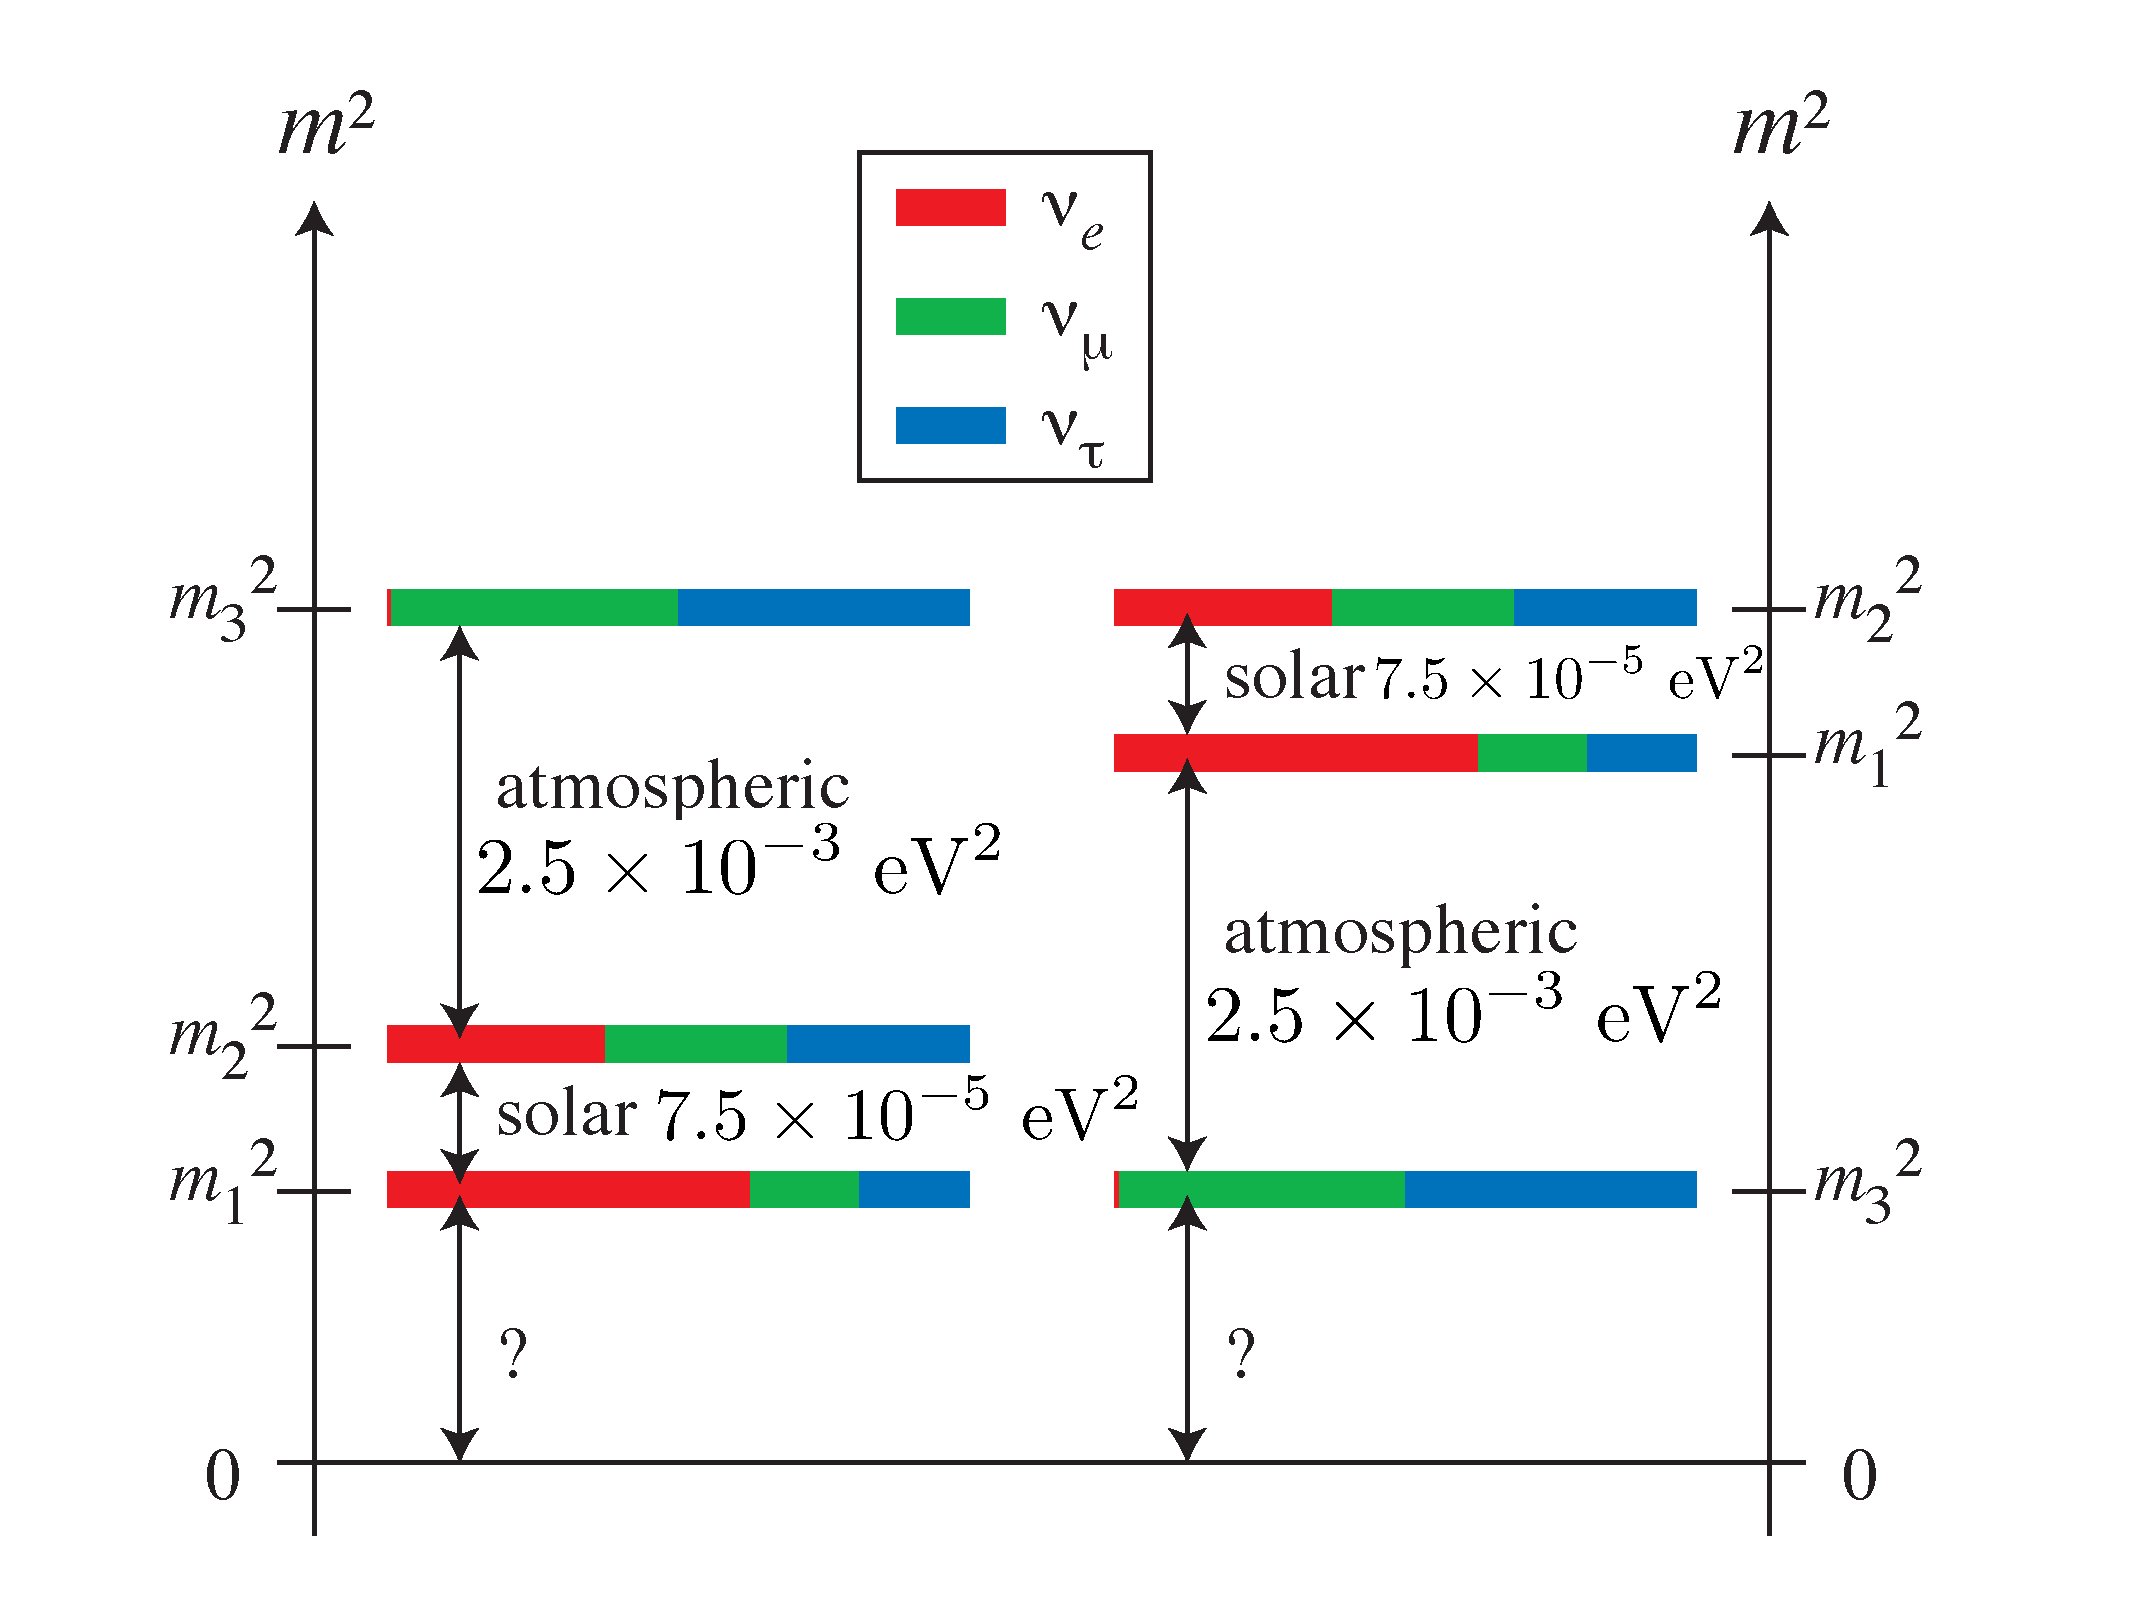
\includegraphics[width=\textwidth]{nu-detection/mass}
	\caption[Neutrino mass ordering]{%
		The two possible neutrino mass orderings arising from the unknown sign of $\dms_{31}$: normal ordering (NO) on the left and inverted ordering (IO) on the right.
		Neutrino oscillation experiments can only determine $\dms_{ij} = m_i ^ 2 - m_j ^ 2$, not the absolute mass scale.
		Also shown is the flavour content (colour bars) of the three mass eigenstates.~\cite{king}
	}
	\label{fig:nu-detection_mass}
\end{figure}

Neutrino oscillation is different in matter than in vacuum.
The neutrinos are coherently scattered off the shell electrons, similar to the propagation of light through matter.
As will be shown in Section~\ref{sec:nu-detection_interactions}, the interactions of \Pgne and \Pagne differ from the other flavours, they are possible through an additional channel.
Thus, the interaction probability of electron neutrinos is higher.
From Figure~\ref{fig:nu-detection_mass}, it can be seen, that \Pgne are primarily present in \HepParticle{\nu}{1}{} and \HepParticle{\nu}{2}{}.
Therefore, the propagation of these two is altered while \HepParticle{\nu}{3}{} is almost unaffected.
Named after its discoverers, the \gls{msw} effect~\cite{mikheyevSmirnov, wolfenstein} can be exploited to determine the mass ordering with a properly tuned $\frac{L}{E}$.


\section{\glsentryshort{dune}}
\label{sec:nu-detection_dune}
\glsreset{dune}
\glsreset{nd}
\glsreset{fd}
\glsreset{surf}

The \dune{}~\cite{dune1, dune2, dune3, dune4} is a long-baseline neutrino oscillation experiment measuring $P \qty(\Pgngm \rightarrow \Pgne)$ and $P \qty(\Pagngm \rightarrow \Pagne)$ planned to start data taking after 2025.
It consist of a neutrino beamline at \gls{fail} in Illinois, USA and a \lartpc{} \gls{fd} at a baseline of \SI{1300}{\kilo\metre} in the \gls{surf} in South Dakota, USA.
An artistic view of \dune{} is shown in Figure~\ref{fig:nu-detection_dune}.

\begin{figure}[htb]
	\centering
	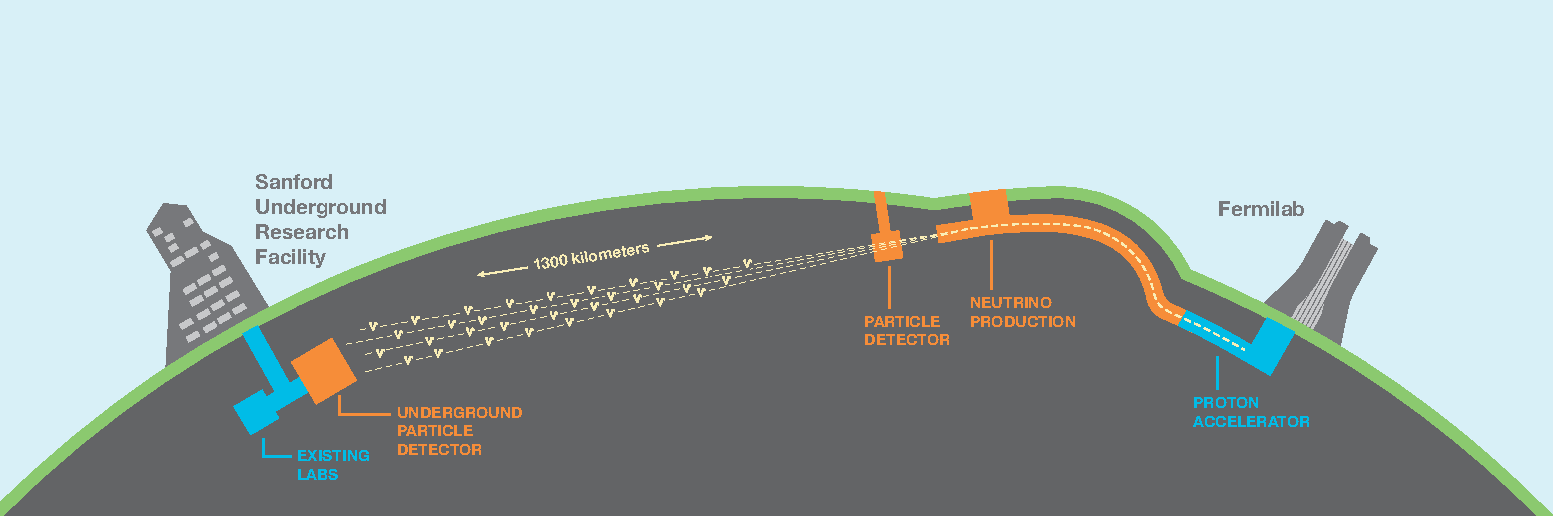
\includegraphics[width=\textwidth]{dune/dune}
	\caption[\glsentryshort{dune}]{%
		\acrshort{dune}, a next-generation long-baseline neutrino oscillation experiment consisting of a neutrino beamline and \acrshort{nd} complex at \acrshort{fail}, and \acrshort{lartpc} \acrshortpl{fd} at \acrshort{surf}.~\cite{dune1}
	}
	\label{fig:nu-detection_dune}
\end{figure}

The beamline at \gls{fail} produces pions by shooting a pulsed proton beam onto a graphite target.
A variable proton energy of \SIrange{60}{120}{\giga\electronvolt} allows for the production of different neutrino fluxes.
One pulse is called a spill and has a duration of \SI{10}{\micro\second} at a period of \SIrange{0.7}{1.2}{\second}, depending on the proton energy.
During phase one of the experiment, each spill will contain \num{7.5e13} protons resulting in an beam power of \SIrange{1.03}{1.20}{\mega\watt}.
In a later phase two, the number of protons per spill will be doubled, doubling the power as well as the average number of events per spill in the detectors.
A summary of the various proton beam configurations is given in Table~\ref{tab:nu-detection_beam-params}.
In accordance with \cite{dune2}, most calculations in this work assume the \SI{2}{\mega\watt} \SI{80}{\giga\electronvolt} beam, i.e. \num{0.2} events per tonne of argon and beam spill.
The produced pions pass through several \gls{em} focusing horns to enter a decay pipe where they decay to \Pgmp(\Pgmm) and \Pgngm(\Pagngm) according to Equation~\eqref{eq:nu-detection_pion-decay}.
By altering the polarity of the current in the focusing horns, either \Pgpp or \Pgpm can be selected primlarily, enhancing the \Pgngm or \Pagngm content of the beam, respectively.
Alongside the pions, a small amount of kaons is produced as well.
These in turn can decay to \Pgne and \Pagne with a branching ratio of $\approx\SI{5}{\percent}$~\cite{pdg} producing a significant \Pgne (\Pagne) beam contamination.
The (anti)neutrino beam flux is depicted in Figure~\ref{fig:nu-detection_dune-flux}.
More information on the beamline can be found in~\cite{dune2}.

\begin{table}[htb]
	\begin{minipage}{\textwidth}
		\centering
		\caption[\glsentryshort{dune} beam parameters and \glsentryshort{nd} rates]{%
			Summary of the \acrshort{dune} proton beam parameters for various configurations.
			Initially, the beamline will operate with the phase one parameters.
			Later, it will be upgraded to support the phase two parameters.
			The spill duration is \SI{10}{\micro\second} for all configurations.
			The last column gives the expected total number of neutrino interactions per tonne of argon and beam spill in the \acrshort{nd}, excluding rock events.
			It is calculated by multiplying the expected neutrino flux with the cross-section on argon from the GENIE\footnote{\url{https://genie.hepforge.org}} neutrino event generator.
			Note that these values are slightly different from the ones in Table~\ref{tab:nu-detection_beam-params} because the latter are outdated.
			In accordance with \cite{dune2}, most calculations in this work assume the \SI{2}{\mega\watt} \SI{80}{\giga\electronvolt} beam, i.e. \num{0.2} events per tonne of argon and beam spill.
			Taken from~\cite{dune3, lauraNDRates}.
		}
		\label{tab:nu-detection_beam-params}
		\begin{tabu} to \textwidth {cSSSSS}
			\toprule
			Phase &			{$E_{\Pp} \ \qty[\si{\giga\electronvolt}]$} &	{\acrshort{pot} per spill} &	{Spill period $\qty[\si{\second}]$} &	{Power $\qty[\si{\mega\watt}]$} &	{\acrshort{nd} rate $\qty[\si{evt\per\tonne_{\ce{Ar}}}]$} \\
			\midrule
			\Romannum{1} &	60 &											7.5e13 &						0.7 &									1.03 &								0.078 \\
			\Romannum{2} &	60 &											1.5e14 &						0.7 &									2.06 &								0.16 \\
			\Romannum{1} & 	80 &											7.5e13 &						0.9 &									1.07 &								0.11 \\
			\Romannum{2} &	80 &											1.5e14 &						0.9 &									2.14 &								0.21 \\
			\Romannum{1} &	120 &											7.5e13 &						1.2 &									1.20 &								0.17 \\
			\Romannum{2} &	120 &											1.5e14 &						1.2 &									2.40 &								0.33 \\
			\bottomrule
		\end{tabu}
	\end{minipage}
\end{table}

\begin{figure}[htb]
	\centering
	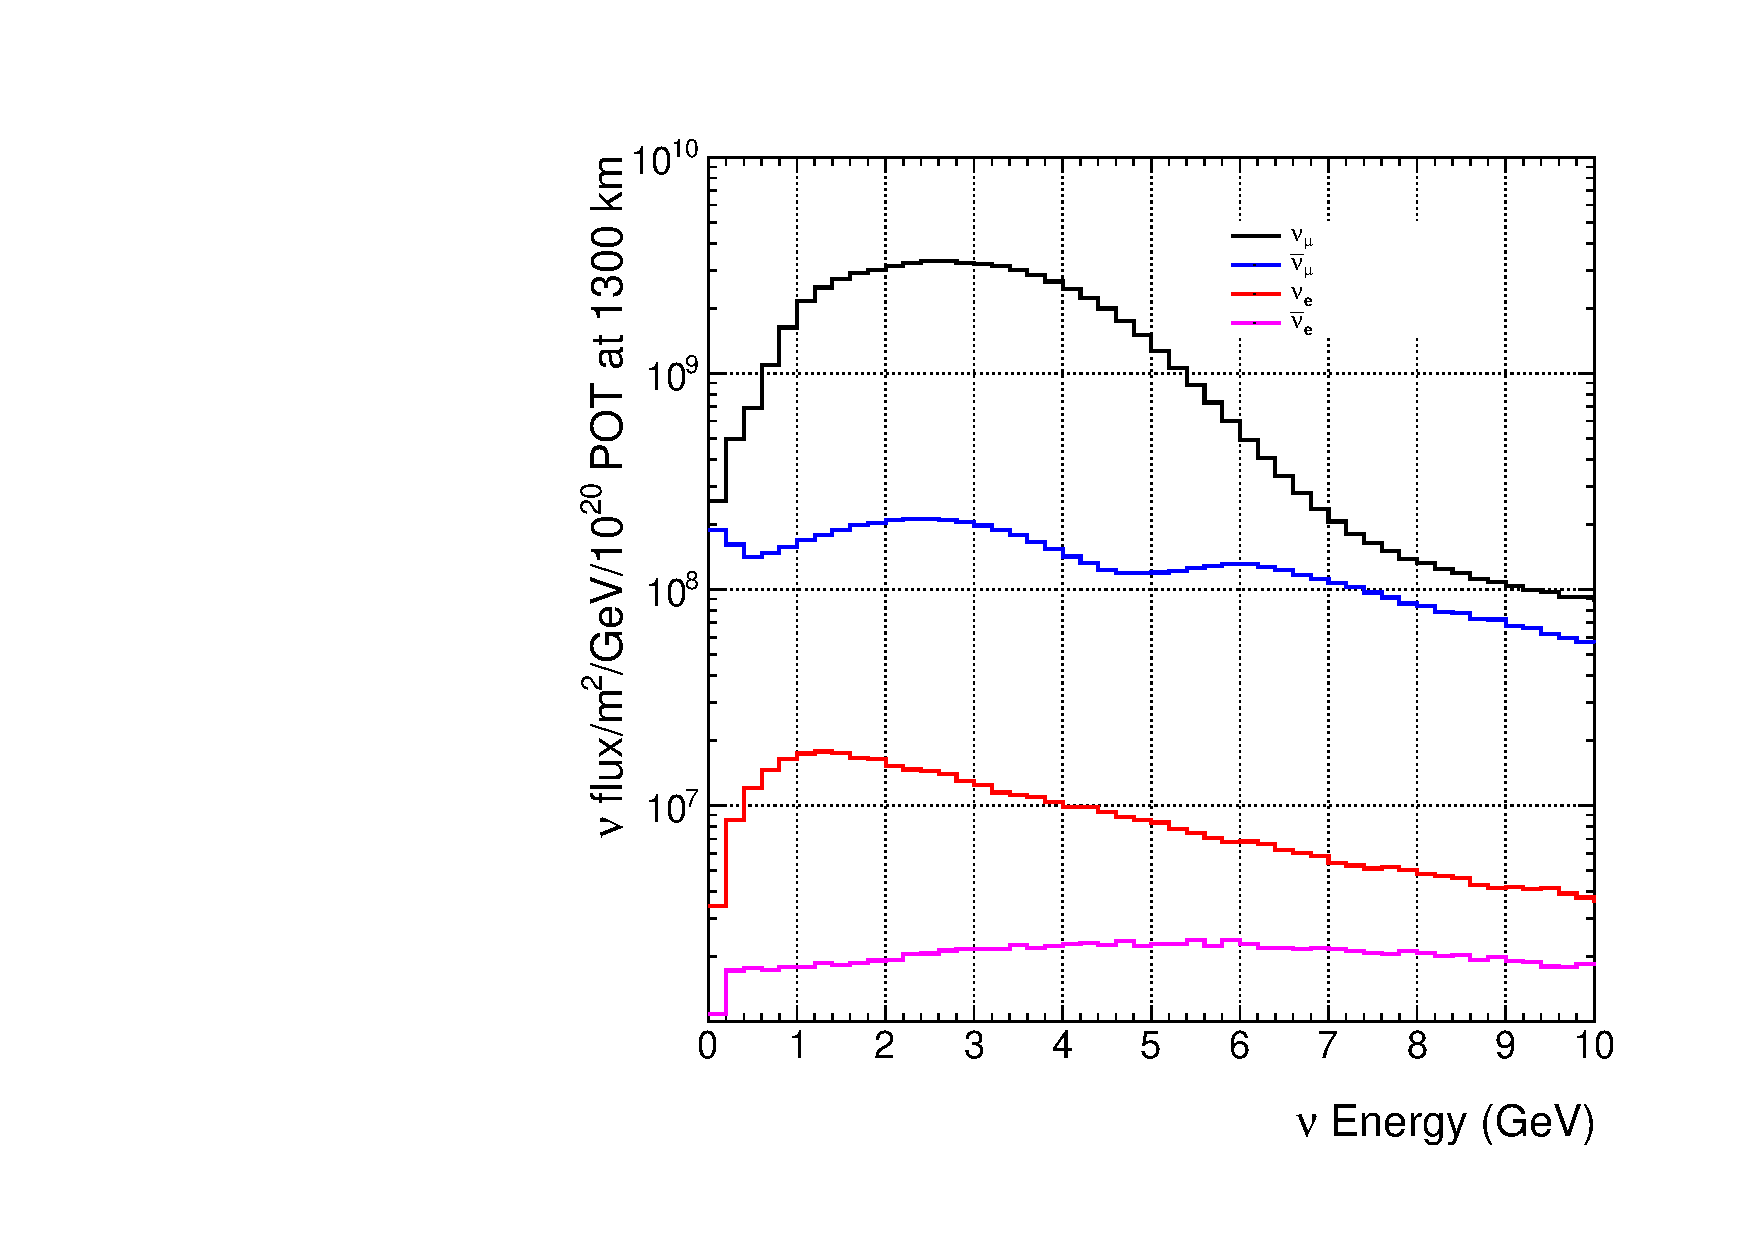
\includegraphics[width=.49\textwidth]{dune/FHC_230kA}
	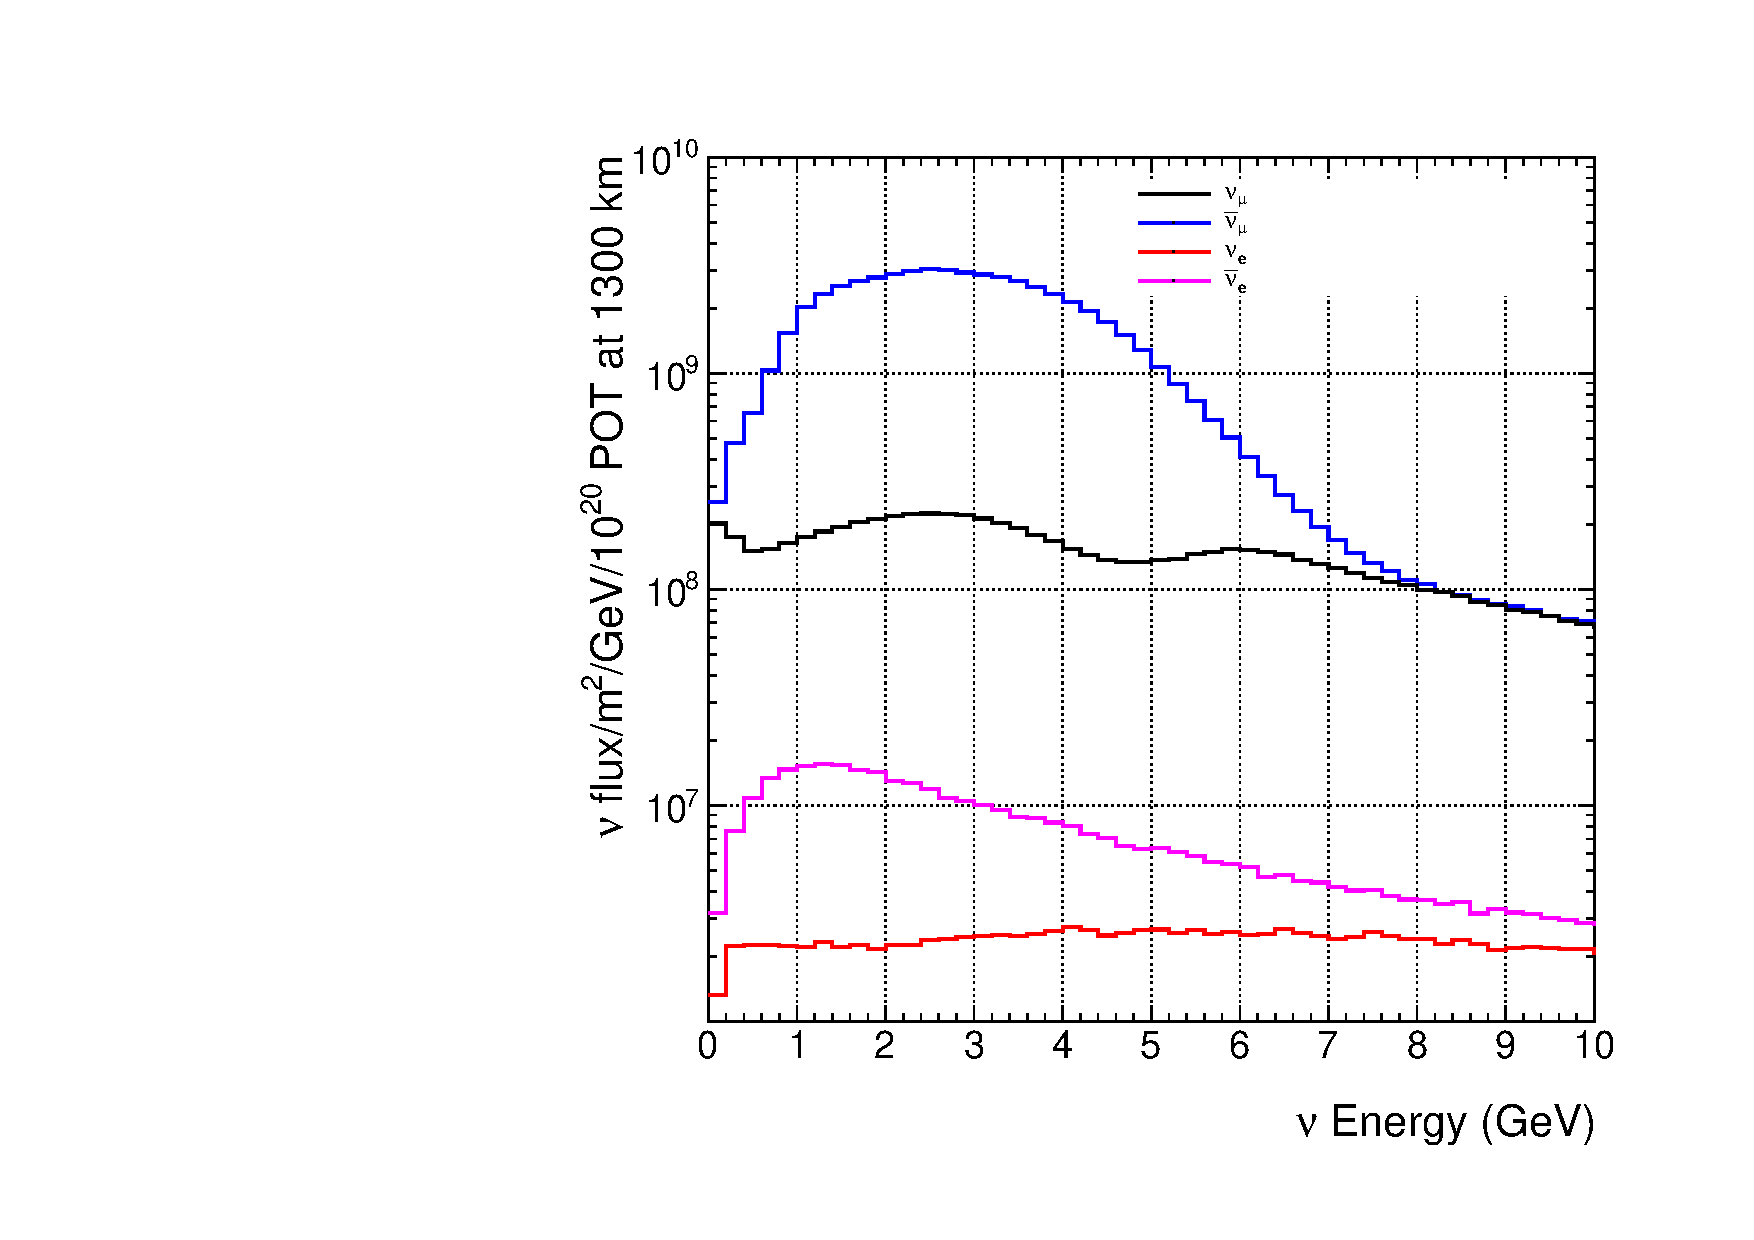
\includegraphics[width=.49\textwidth]{dune/RHC_230kA}
	\caption[\glsentryshort{dune} neutrino fluxes.]{%
		Neutrino fluxes for the \acrshort{dune} reference beam design operating in neutrino mode (left) and antineutrino mode (right), generated with a \SI{120}{\giga\electronvolt} primary proton beam.~\cite{dune2}
	}
	\label{fig:nu-detection_dune-flux}
\end{figure}

The baseline and energy spectrum of \dune{} are optimised to measure \dcp{} and determine the mass ordering.
Figure~\ref{fig:nu-detection_dune-osc} shows the (anti)neutrino oscillation probability as a function of neutrino energy at the \dune{} baseline for the normal and inverted mass ordering.
Put into very simple terms, \dcp{} can be derived from the difference in oscillation probability between neutrino and antineutrino mode.
The \gls{msw} effect enhances either neutrino or antineutrino oscillation depending on the mass ordering, allowing for a determination of the latter.
For more thorough sensitivity treatments, see~\cite{king, duneT2HKSens, qianVogel}.

\begin{figure}[htb]
	\centering
	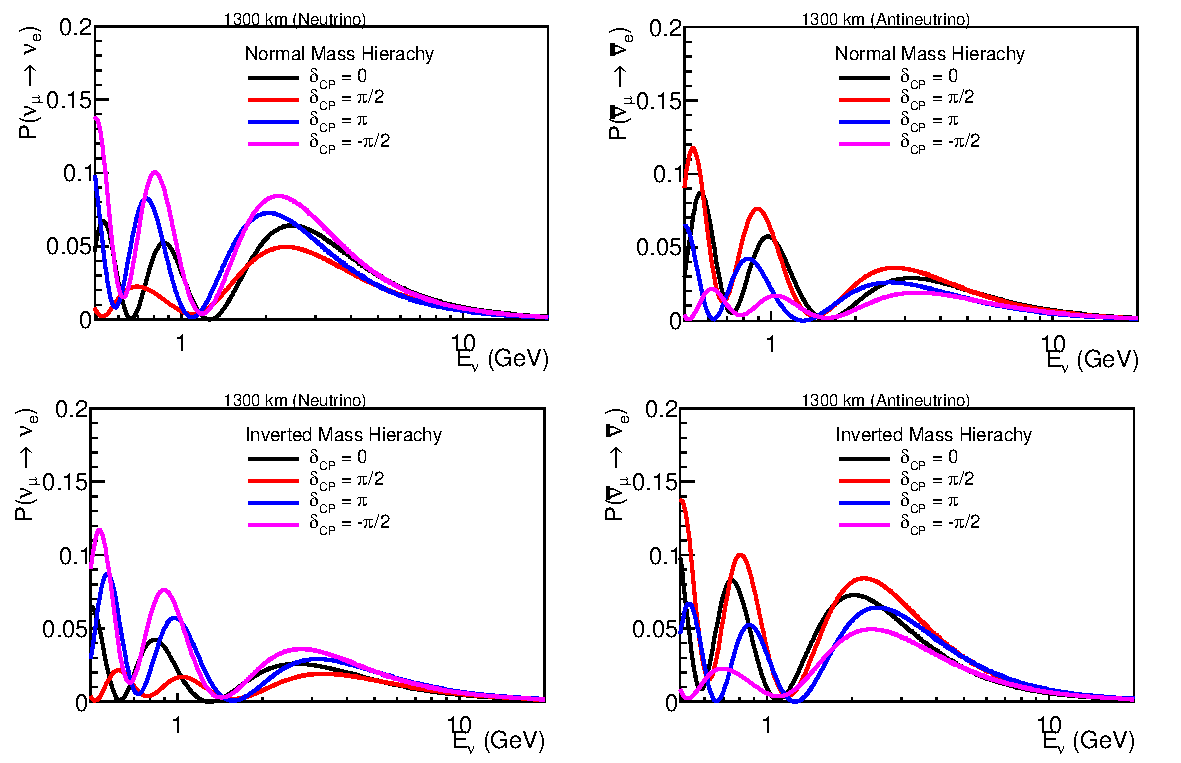
\includegraphics[width=\textwidth]{dune/LBNE_osc}
	\caption[Neutrino oscillation probabilities.]{%
		Muon to electron neutrino (left) and antineutrino (right) oscillation probability for normal (top) and inverted (bottom) mass ordering (hierarchy in the figure).
		The oscillation probabilities are calculated from equation~\eqref{eq:nu-detection_oscprob}.
		\dcp{} can be obtained from the difference between neutrino and antineutrino mode.
		The \acrshort{msw} effect either enhances the probability in neutrino or antineutrino mode depending on the mass ordering, allowing for a determination or the latter.~\cite{qianVogel}
	}
	\label{fig:nu-detection_dune-osc}
\end{figure}

Figure~\ref{fig:nu-detection_dune-sens} shows the sensitivities of \dune{} to determination of the mass ordering and discovery of \gls{cp} violation.
To reach a $3 \sigma$ sensitivity for a \SI{75}{\percent} coverage of the \dcp{} parameter space, an exposure of \SI{1320}{\kilo\tonne\mega\watt.years} is required.
Assuming the reference design of a \SI{40}{\kilo\tonne} \gls{fd} and a \SI{1}{\mega\watt} beam results in a data taking time of \SI{33}{years}.
Therefore, to reach the sensitivity goal earlier, a beam $> \SI{1}{\mega\watt}$ is required.

\begin{figure}[htb]
	\centering
	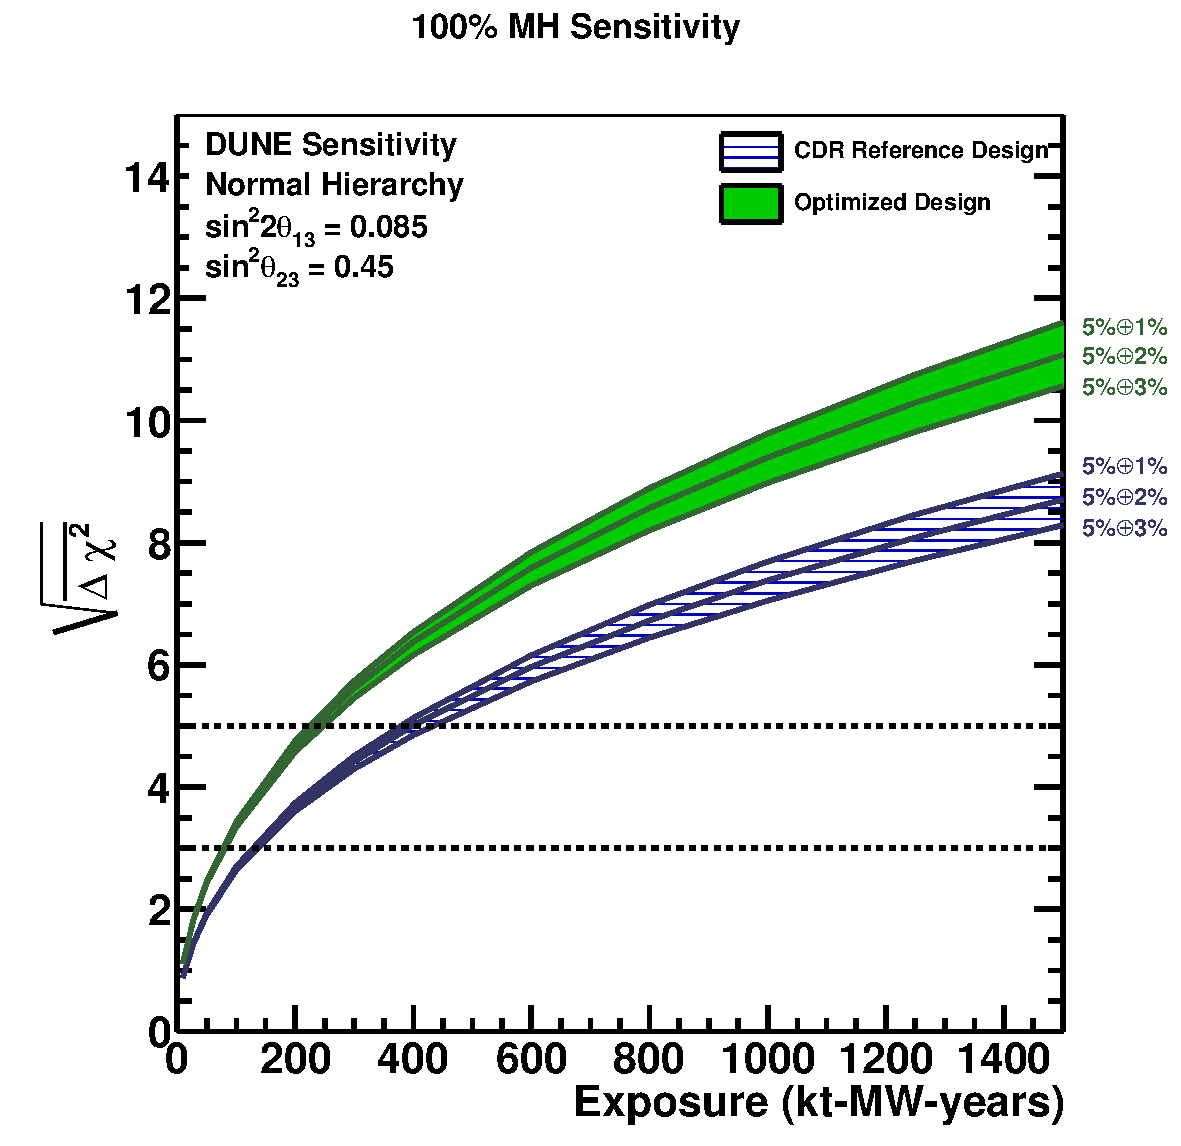
\includegraphics[width=.49\textwidth]{dune/mh_exp_syst}
	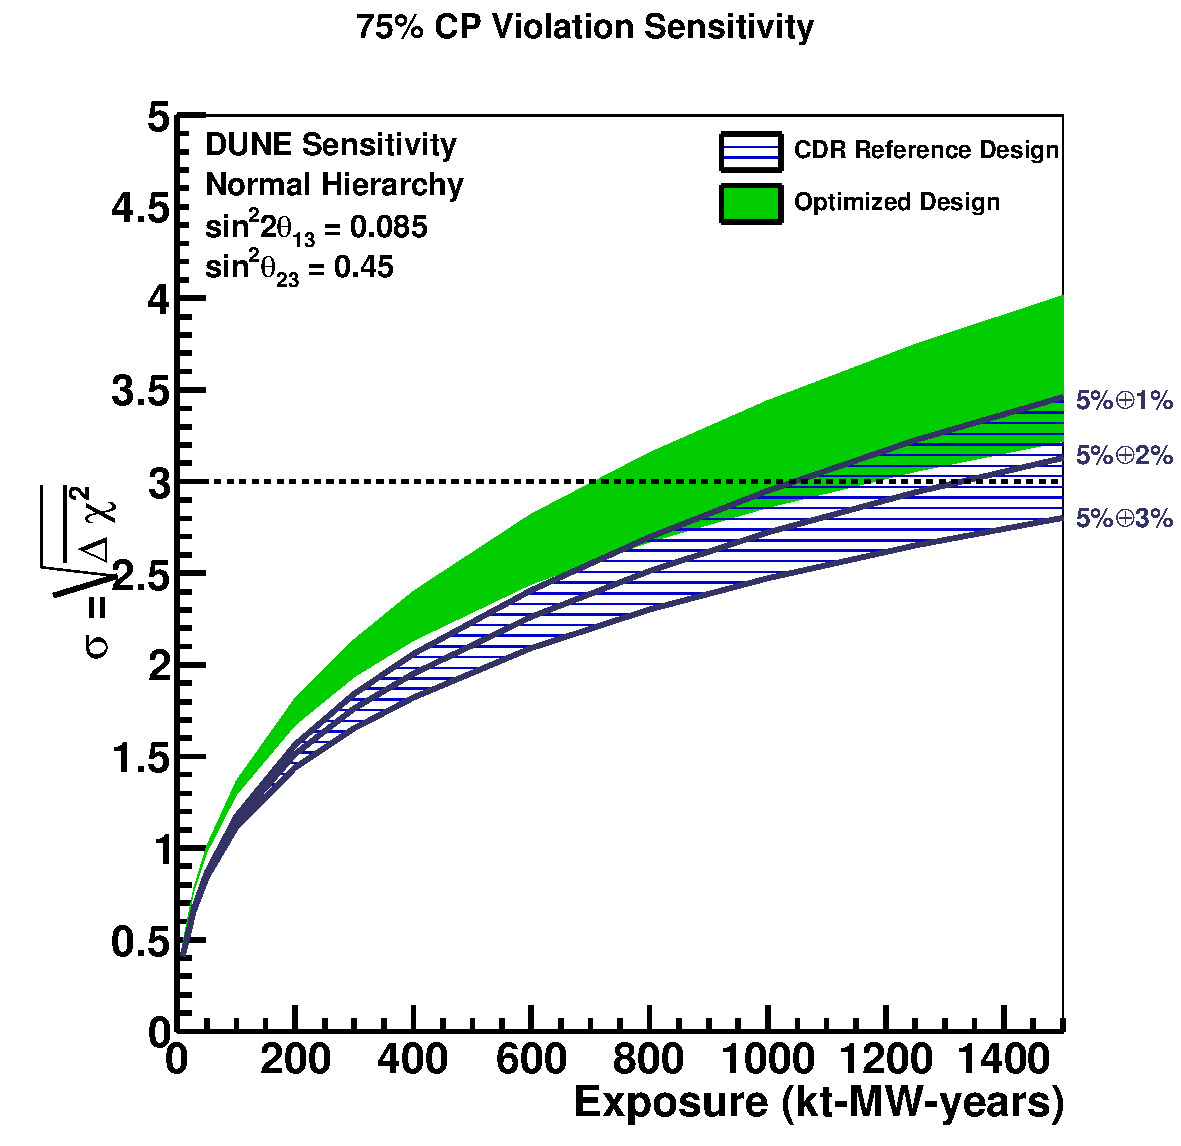
\includegraphics[width=.49\textwidth]{dune/cpv75_exp_syst}
	\caption[\glsentryshort{dune} \dcp{} sensitivity]{%
		Expected sensitivity of \acrshort{dune} to determination of the neutrino mass ordering (hierarchy, left) and discovery of \acrshort{cp} violation, i.e.\ $\dcp \neq\ 0\ \m{or}\ \pi$, (right) as a function of exposure in \si{\kilo\tonne\mega\watt.years}, assuming equal running in neutrino and antineutrino mode, for a range of values for the \Pgne and \Pagne signal normalisation uncertainties from $\SI{5}{\percent}\oplus\SI{3}{\percent}$ to $\SI{5}{\percent}\oplus\SI{1}{\percent}$.
		The sensitivities quoted are the minimum sensitivity for \SI{100}{\percent} of \dcp{} values in the case of mass ordering and \SI{75}{\percent} of \dcp{} values in the case of \acrshort{cp} violation.
		The two bands on each plot represent a range of potential beam designs described in \cite{dune2}: the blue hashed band is for the reference design and the solid green band is for the optimized design.
		For \acrshort{cp} violation sensitivities, true mass ordering is assumed to be normal but unknown.
		Taken from~\cite{dune2}.
	}
	\label{fig:nu-detection_dune-sens}
\end{figure}

Another important feature of Figure~\ref{fig:nu-detection_dune-sens} are the indicated signal normalisation uncertainties.
In particular the second number has a significant influence on sensitivity, the aforementioned exposure assumes an uncertainty of $\SI{5}{\percent}\oplus\SI{2}{\percent}$.
A detailed explanation of this is out of the scope of this work and can be found in~\cite{dune2}.
What shall be mentioned here however is that these uncertainties can be reached by a precise constraint of the flux rate and shape by means of a \gls{nd}.
It is placed at a distance of \SI{574}{\metre} downstream of the proton beam target.
To eliminate the introduction of further extrapolation uncertainties it is important to have a \gls{nd} component employing the same target material and detector technology as the \gls{fd}, i.e.\ a \lartpc{}.

As will be explained in Chapter~\ref{chap:lartpc}, \lartpc{}s are slow detectors.
This is problematic in the high-multiplicity \gls{nd} environment of \dune{} which is the reason why~\cite{dune2} and~\cite{dune4} do not mention an \gls{nd} \lar{} component.
The aforementioned \si{\mega\watt} beam intensity leads to \gls{nd} event rates of \num{0.2} events per tonne of argon leading to significant event pile-up (see Table~\ref{tab:nu-detection_beam-params}).
Rock events---secondary particles produced by beam neutrino interactions in the surrounding material, entering the detector---are not included in this estimate.


\section{Neutrino Interaction with Matter}
\label{sec:nu-detection_interactions}
\glsreset{cc}
\glsreset{nc}
\glsreset{qe}
\glsreset{res}
\glsreset{dis}
\glsreset{coh}
\glsreset{mec}

\begin{table}[htb]
	\centering
	\caption[\glsentryshort{dune} \glsentryshort{nd} event rates]{%
		Estimated number of interactions per tonne of argon at the \acrshort{dune} \acrshort{nd} for approximately one month (\num{1e20}~\acrshort{pot}) exposure to an (anti)neutrino beam produced from a primary proton beam of \SI{120}{\giga\electronvolt} and \SI{1.2}{\mega\watt}, taken from~\cite{dune2}.
		Note that these rates are slightly different from the ones in Table~\ref{tab:nu-detection_beam-params}.
		The reason for this is that the values below are outdated.
		However, their order of magnitude is correct and no such detailed breakdown is available for the more recent values.
		Therefore, they are presented as a rough estimate for the expected rates for the different interaction channels.
	}
	\label{tab:nu-detection_nd-rates}
	\begin{tabu} to \textwidth {llSS}
		\toprule
		Production mode &		Reaction &																														{\Pgngm beam} &		{\Pagngm beam} \\
		\midrule
		\acrshort{cc} \acrshort{qe} &			\HepProcess{\Pgngm\Pn \to \Pgmm\Pp} &																			30000 &				13000 \\
		\acrshort{nc} elastic &					\HepProcess{\Pgngm\nucleon \to \Pgngm\nucleon} & 																11000 &				6700 \\
		\acrshort{cc} \acrshort{res} &			\HepProcess{\Pgngm\Pp \to \Pgmm\Pp\Pgpp} &																		21000 &				0 \\
		\acrshort{cc} \acrshort{res} &			\HepProcess{\Pgngm\Pn \to \Pgmm\Pn\Pgpp\, (\Pp\Pgpz)} &															23000 &				0 \\
		\acrshort{cc} \acrshort{res} &			\HepProcess{\Pagngm\Pp \to \Pgmp\Pp\Pgpm\, (\Pn\Pgpz)} &														0 &					8300 \\
		\acrshort{cc} \acrshort{res} &			\HepProcess{\Pagngm\Pn \to \Pgmp\Pn\Pgpm} &																		0 &					12000 \\
		\acrshort{nc} \acrshort{res} &			\HepProcess{\Pgngm\Pp \to \Pgngm\Pp\Pgpz\, (\Pn\Pgpp)} &														7000 &				0 \\
		\acrshort{nc} \acrshort{res} &			\HepProcess{\Pgngm\Pn \to \Pgngm\Pn\Pgpp\, (\Pp\Pgpz)} &														9000 &				0 \\
		\acrshort{nc} \acrshort{res} &			\HepProcess{\Pagngm\Pp \to \Pagngm\Pp\Pgpm\, (\Pn\Pgpz)} &														0 &					3900 \\
		\acrshort{nc} \acrshort{res} &			\HepProcess{\Pagngm\Pn \to \Pagngm\Pn\Pgpm} &																	0 &					4700 \\
		\acrshort{cc} \acrshort{dis} &			\HepProcess{\Pgngm\nucleon \to \Pgmm\particles} or \HepProcess{\Pagngm\nucleon \to \Pgmp\particles} &			95000 &				24000 \\
		\acrshort{nc} \acrshort{dis} &			\HepProcess{\Pgngm\nucleon \to \Pgngm\particles} or \HepProcess{\Pagngm\nucleon \to \Pagngm\particles} &		31000 &				10000 \\
		\acrshort{cc} \acrshort{coh} \Pgpp &	\HepProcess{\Pgngm\nucleus \to \Pgmm\nucleus\Pgpp} &															930 &				0 \\
		\acrshort{cc} \acrshort{coh} \Pgpm &	\HepProcess{\Pagngm\nucleus \to \Pgmp\nucleus\Pgpm} &															0 &					800 \\
		\acrshort{nc} \acrshort{coh} \Pgpz &	\HepProcess{\Pgngm\nucleus \to \Pgngm\nucleus\Pgpz} or \HepProcess{\Pagngm\nucleus \to \Pagngm\nucleus\Pgpz} &	520 &				450 \\
		\acrshort{nc} elastic electron &		\HepProcess{\Pgngm\Pem \to \Pgngm\Pem} or \HepProcess{\Pagngm\Pem \to \Pagngm\Pem} &							16 &				11 \\
		Inverse muon decay &					\HepProcess{\Pgngm\Pem \to \Pgmm\Pgne} &																		9.5 &				0 \\
		\midrule
		Total \acrshort{cc} &			&																														170000 &			59000 \\
		Total \acrshort{cc}+\acrshort{nc} &	&																													230000 &			84000 \\
		\bottomrule
	\end{tabu}
\end{table}

Neutrinos cannot be directly detected, they need to pass on some of their energy and momentum to secondary particles that can be detected, i.e.\ they need to interact with a detection medium.
This chapter will give a brief overview of the different types of these interactions.
In general, neutrino interactions are divided into \gls{cc} and \gls{nc} mediated by charged (\PWpm) or neutral (\PZz) gauge bosons.
In a \gls{cc} interaction, the neutrino is transformed into its corresponding charged lepton while it survives an \gls{nc} interaction.
Furthermore, they can be subdivided according to the type of interaction into \gls{qe}, \gls{res}, \gls{dis}, and \gls{coh}.

\gls{qe} is characterised by the reactions
\begin{IEEEeqnarray}{C}
	\HepProcess{\Pgnl\Pn \to \Plm\Pp} \qand \HepProcess{\Pagnl\Pp \to \Plp\Pn}
\end{IEEEeqnarray}
and the kinematics are similar to that of an elastic collision, hence called \gls{qe}.
Apparent from the equation above, this can only happen as a \gls{cc} interaction.

The \gls{nc} equivalent is an actual elastic interaction of a neutrino with a target nucleon according to
\begin{IEEEeqnarray}{C}
	\HepProcess{\Pgnl\nucleon \to \Pgnl\nucleon} \qq*{.}
\end{IEEEeqnarray}

\gls{res} involves the excitation of the involved nucleon to a resonant state, e.g.\
\begin{IEEEeqnarray}{C}
	\HepProcess{\Pgngm\Pp \to \Pgmm\HepParticle{\Delta}{}{++} \to \Pgmm\Pp\Pgpp}
\end{IEEEeqnarray}
where the \HepParticle{\Delta}{}{++} resonance is too short-lived to be seen by the detectors.
There are a lot of different \gls{res} interactions which all work in a similar manner.

For \gls{dis}, the momentum transfer is high enough to destroy nucleon.
The neutrino rips a quark out which, in turn, starts to hadronise and form jets.
The reactions are
\begin{IEEEeqnarray}{C}
	\HepProcess{\Pgnl\nucleon \to \Pl\particles} \qor \HepProcess{\Pgnl\nucleon \to \Pgnl\particles}
\end{IEEEeqnarray}
where \nucleon is the target nucleon and \particles a group of hadrons.
This reaction happens in a very similar manner to deep inelastic electron scattering off nucleons.

In a \gls{coh} reaction, the opposite happens.
The neutrino interacts with a target nucleus ($A$) as a whole but the latter is left intact as a spectator.
Instead, another particle is produced alongside the corresponding lepton. An example reaction is
\begin{IEEEeqnarray}{C}
	\HepProcess{\Pgngm\nucleus \to \Pgngm\nucleus\Pgpz}
\end{IEEEeqnarray}
where a pion is produced from a muon neutrino interacting with a target nucleus.

The inverse muon decay,
\begin{IEEEeqnarray}{C}
	\HepProcess{\Pgngm\Pem \to \Pgmm\Pgne} \qc
\end{IEEEeqnarray}
requires neutrino energies above \SI{11}{\giga\electronvolt}~\cite{dune2}.

Of particular importance is elastic scattering off shell electrons,
\begin{IEEEeqnarray}{C}
	\HepProcess{\Pgnl\Pem \to \Pgnl\Pem} \qor \HepProcess{\Pagnl\Pem \to \Pagnl\Pem} \qc
\end{IEEEeqnarray}
which is possible for all (anti)neutrino flavours.
For \Pgne/\Pagne, the interaction is also possible in the \gls{cc} channel via the exchange of a \PWpm boson as depicted in Figures~\ref{fig:nu-detection_nue-scat} and~\ref{fig:nu-detection_nueb-scat}.
This gives rise to a flavour-dependent term in the oscillation probability in matter, the \gls{msw} effect (see Section~\ref{sec:nu-detection_osc}).

\begin{figure}[htb]
	\centering
	\begin{fmffile}{graphics/fmf/NC-nue-scat}
		\unitlength=.4\textwidth
		\begin{fmfgraph*}(1,.5)
			\fmfpen{thin}
			\fmfstraight
			\fmfleftn{i}{2}
			\fmfrightn{o}{2}
			\fmf{fermion,label=\Pem,label.side=left}{i1,v1}
			\fmf{fermion,label=\Pem,label.side=left}{v1,o1}
			\fmf{fermion,label=\Pgnl,label.side=right}{i2,v2}
			\fmf{fermion,label=\Pgnl,label.side=right}{v2,o2}
			\fmf{boson,label=\PZz,label.side=left}{v1,v2}
			\fmfdot{v1,v2}
		\end{fmfgraph*}
	\end{fmffile}
	\begin{fmffile}{graphics/fmf/CC-nue-scat}
		\unitlength=.4\textwidth
		\begin{fmfgraph*}(1,.5)
			\fmfpen{thin}
			\fmfstraight
			\fmfleftn{i}{2}
			\fmfrightn{o}{2}
			\fmf{fermion,label=\Pem,label.side=left}{i1,v1}
			\fmf{fermion,label=\Pgne,label.side=left}{v1,o1}
			\fmf{fermion,label=\Pgne,label.side=right}{i2,v2}
			\fmf{fermion,label=\Pem,label.side=right}{v2,o2}
			\fmf{boson,label=\PWpm,label.side=left}{v1,v2}
			\fmfdot{v1,v2}
		\end{fmfgraph*}
	\end{fmffile}
	\caption[Neutrino electron scattering]{%
		\acrshort{nc} (left) and \acrshort{cc} (right) neutrino electron scattering.
	}
	\label{fig:nu-detection_nue-scat}
\end{figure}

\begin{figure}[htb]
	\centering
	\begin{fmffile}{graphics/fmf/NC-nueb-scat}
		\unitlength=.4\textwidth
		\begin{fmfgraph*}(1,.5)
			\fmfpen{thin}
			\fmfstraight
			\fmfleftn{i}{2}
			\fmfrightn{o}{2}
			\fmf{fermion,label=\Pem,label.side=left}{i1,v1}
			\fmf{fermion,label=\Pem,label.side=left}{v1,o1}
			\fmf{fermion,label=\Pagnl,label.side=right}{i2,v2}
			\fmf{fermion,label=\Pagnl,label.side=right}{v2,o2}
			\fmf{boson,label=\PZz,label.side=left}{v1,v2}
			\fmfdot{v1,v2}
		\end{fmfgraph*}
	\end{fmffile}
	\begin{fmffile}{graphics/fmf/CC-nueb-scat}
		\unitlength=.4\textwidth
		\begin{fmfgraph*}(1,.5)
			\fmfpen{thin}
			\fmfstraight
			\fmfleftn{i}{2}
			\fmfrightn{o}{2}
			\fmf{fermion,label=\Pem,label.side=left}{i1,v1}
			\fmf{fermion,label=\Pem,label.side=left}{v2,o1}
			\fmf{fermion,label=\Pagne,label.side=right}{i2,v1}
			\fmf{fermion,label=\Pagne,label.side=right}{v2,o2}
			\fmf{boson,label=\PWm,label.side=left}{v1,v2}
			\fmfdot{v1,v2}
		\end{fmfgraph*}
	\end{fmffile}
	\caption[Antineutrino electron scattering]{%
		\acrshort{nc} (left) and \acrshort{cc} (right) antineutrino electron scattering.
	}
	\label{fig:nu-detection_nueb-scat}
\end{figure}

A summary of the expected rates of the different interactions in the \dune{} \gls{nd} is given in Table~\ref{tab:nu-detection_nd-rates}.
Figure~\ref{fig:nu-detection_xsec} depicts the cross-section (see next paragraph) of neutrino interactions as a function of neutrino energy.
For comparison, the flux shapes of several experiments are shown (in arbitraty units).
The cross-section is split into contributions from \gls{cc} and \gls{nc} interactions.
For \gls{cc}, the individual contributions from \gls{res} and 1p1h+2p2h are shown.
$x$p$y$h refers to $x$ particles and $y$ holes, i.e.\ the target nucleus is missing $y$ nucleons after the interactions.
1p1h corresponds to a \gls{cc} \gls{qe} interaction whereas in 2p2h interactions, a virtual meson is exchanged inside the target nucleus, also called \gls{mec}.
Interactions involving \glspl{mec} are important because they can mimic the detector response of \gls{cc} \gls{qe} events.

\begin{figure}[htb]
	\centering
	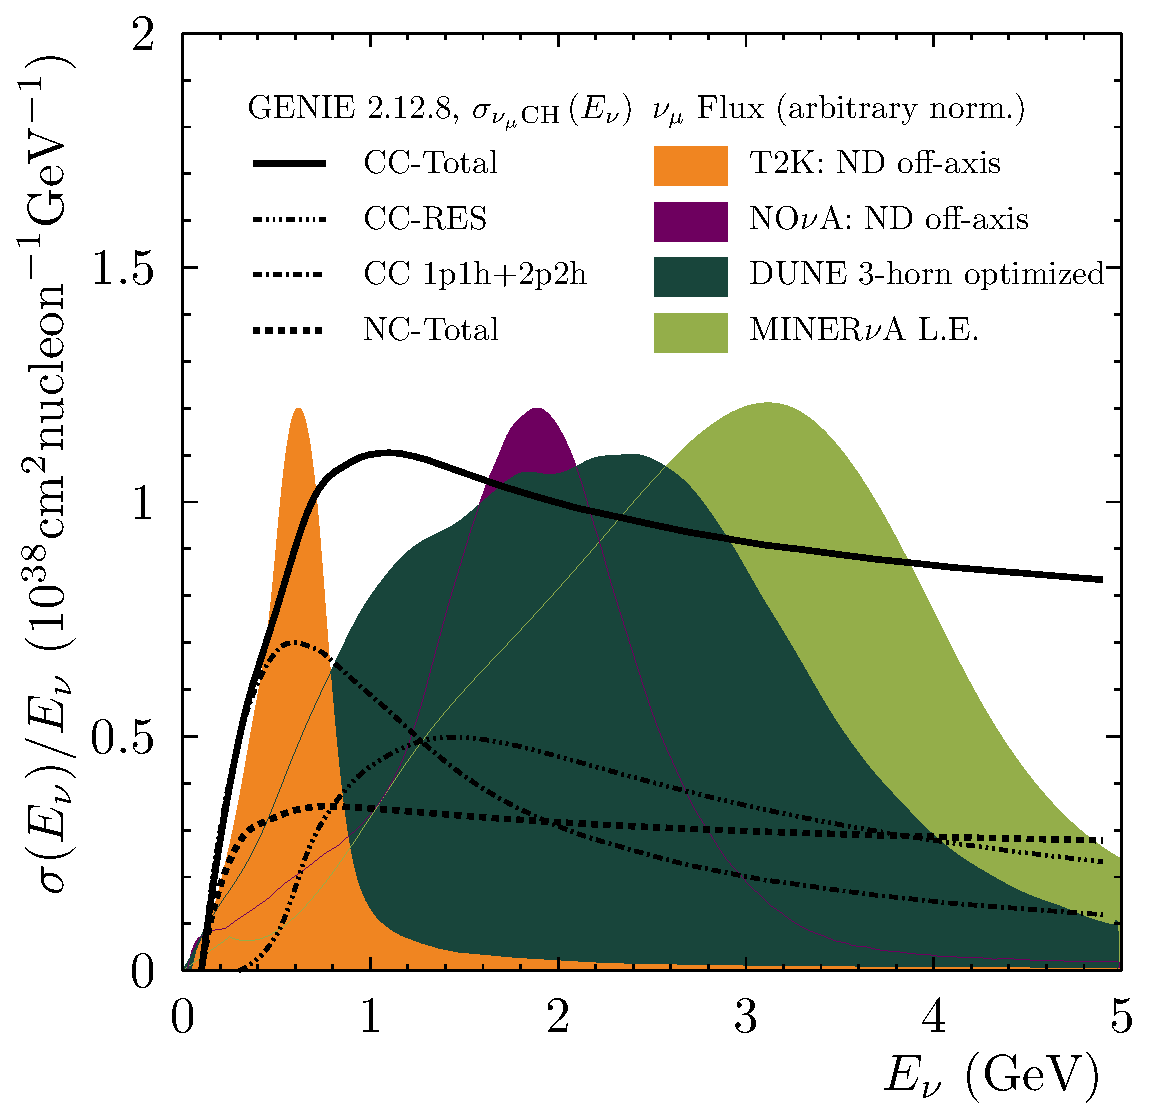
\includegraphics[width=\textwidth]{nu-detection/flux_and_xsec_from_luke}
	\caption[Neutrino interaction cross-section]{%
		Neutrino interaction cross-section per nucleon as a function of neutrino energy in \si{\giga\electronvolt}.
		Overlaid are the flux shapes of various beam experiments in arbitrary units.
		The cross-section is split into contributions from \acrshort{cc} and \acrshort{nc} interactions.
		For \acrshort{cc}, the individual contribution from \acrshort{res} interactions is shown, as well as from the sum of 1p1h and 2p2h. The latter two correspond to the \acrshort{qe} channel and interactions involving \acrshortpl{mec}, respectively.~\cite{xsec_luke}
	}
	\label{fig:nu-detection_xsec}
\end{figure}

To better understand the meaning of Figure~\ref{fig:nu-detection_xsec}, a brief explanation of the cross-section concept is given here.
For a beam consisting of particles \particlea, incident on a target made of particles \particleb, the rate of the interaction \HepProcess{\particlea\particleb \to \particles} is given by
\begin{IEEEeqnarray}{rCl}
	R_{\particles} & = & \phi_{\particlea} N_{\particleb} \sigma_{\particlea\particleb\particles} \qc
\end{IEEEeqnarray}
where $\phi_{\particlea}$ is the flux of beam particles, $N_{\particleb}$ is the number of target particles, and $\sigma_{\particlea\particleb\particles}$ is the cross-section.
Therefore, the cross-section
\begin{IEEEeqnarray}{rCl}
	\sigma_{\particlea\particleb\particles} & = & \frac{R_X}{\phi_{\particlea} N_{\particleb}}
\end{IEEEeqnarray}
is a measure for the interaction rate $R_{\particles}$ normalised by the number of both, beam and target, particles.
As flux is given in units of inverse time and area, and interaction rate in inverse time, the cross-section needs to have the dimension of an area.


\section{Final State Detection}
\label{sec:nu-detection_fs}

In order to be able to detect particles, they need to interact with a detection medium.
This section will describe the most important interaction of charged particles as well as neutral particles with matter.
A special focus is laid on charged interactions as these are the most important ones for \lartpc{}s.
As a measure of the interaction strength, the energy loss per distance or stopping power $\dv{E}{x}$ is used.
Where not otherwise mentioned, this section is based on~\cite{grupen}.

The main interaction of charged particles with matter happens on atomic electrons.
That is why for most of these interactions, one needs to treat the interaction of electrons separately.
For all other charged particles, the stopping power is described by the Bethe-Bloch formula
\begin{IEEEeqnarray}{rCl}
	- \frac{1}{\rho} \dv{E}{x} & = &
	4 \pi N_{\m{A}} r_{\Pe} ^ 2 m_{\Pe} c ^ 2 z ^ 2 \frac{Z}{A} \frac{1}{\beta ^ 2}
	\qty[\ln(\frac{2 m_{\Pe} c ^ 2 \gamma ^ 2 \beta ^ 2}{I}) - \beta ^ 2 - \frac{\delta}{2}] \qc
	\label{eq:nu-detection_bethe-bloch}
\end{IEEEeqnarray}
where
\begin{description}
	\item[$\rho$] is the density of the absorber material,
	\item[$N_{\m{A}}$] is Avogadro's number,
	\item[$r_{\Pe} = \frac{1}{4 \pi \varepsilon_{\m{0}}} \frac{\si{\elementarycharge} ^ 2}{m_{\Pe} c ^ 2}$] is the classical electron radius using the permittivity of free space $\varepsilon_{\m{0}}$,
	\item[$m_{\Pe}$] is the electron mass,
	\item[$z$] is the charge of the incident particle,
	\item[$Z$] is the atomic number of the absorber,
	\item[$A$] is the atomic weight of the absorber,
	\item[$\beta = \frac{v}{c}$] with $v$ the velocity of the incident particle,
	\item[$\gamma = \frac{E}{m_0 c ^ 2}$] with $E$ the energy and $m_0$ the rest mass of the incident particle,
	\item[$I$] is the mean excitation energy of the absorber material which can be approximated by
		\begin{IEEEeqnarray}{rCl}
			I & = & 16 Z ^ {0.9} \si{\electronvolt} \quad \m{for} \quad Z > 1 \qc
		\end{IEEEeqnarray}
	\item[$\delta$] is a parameter describing the screening of the extended transverse electric field of relativistic incident particles by the charge density of the atomic electrons of the absorber.
\end{description}
Equation~\eqref{eq:nu-detection_bethe-bloch} describes the stopping power of particles with $m_0 \gg m_{\Pe}$ by ionisation and excitation of the atoms in the absorber material.
As the stopping power is proportional to the electron density and thus to the mass density of the absorber material, it is often divided by the latter.
Thus, Equation~\eqref{eq:nu-detection_bethe-bloch} actually gives the so called mass stopping power.
The only remaining dependence on the absorber material is $\frac{Z}{A}$ which is $\approx 0.5$ for most light materials, and the mean excitation energy which only contributes logarithmically.

\begin{figure}[htb]
	\centering
	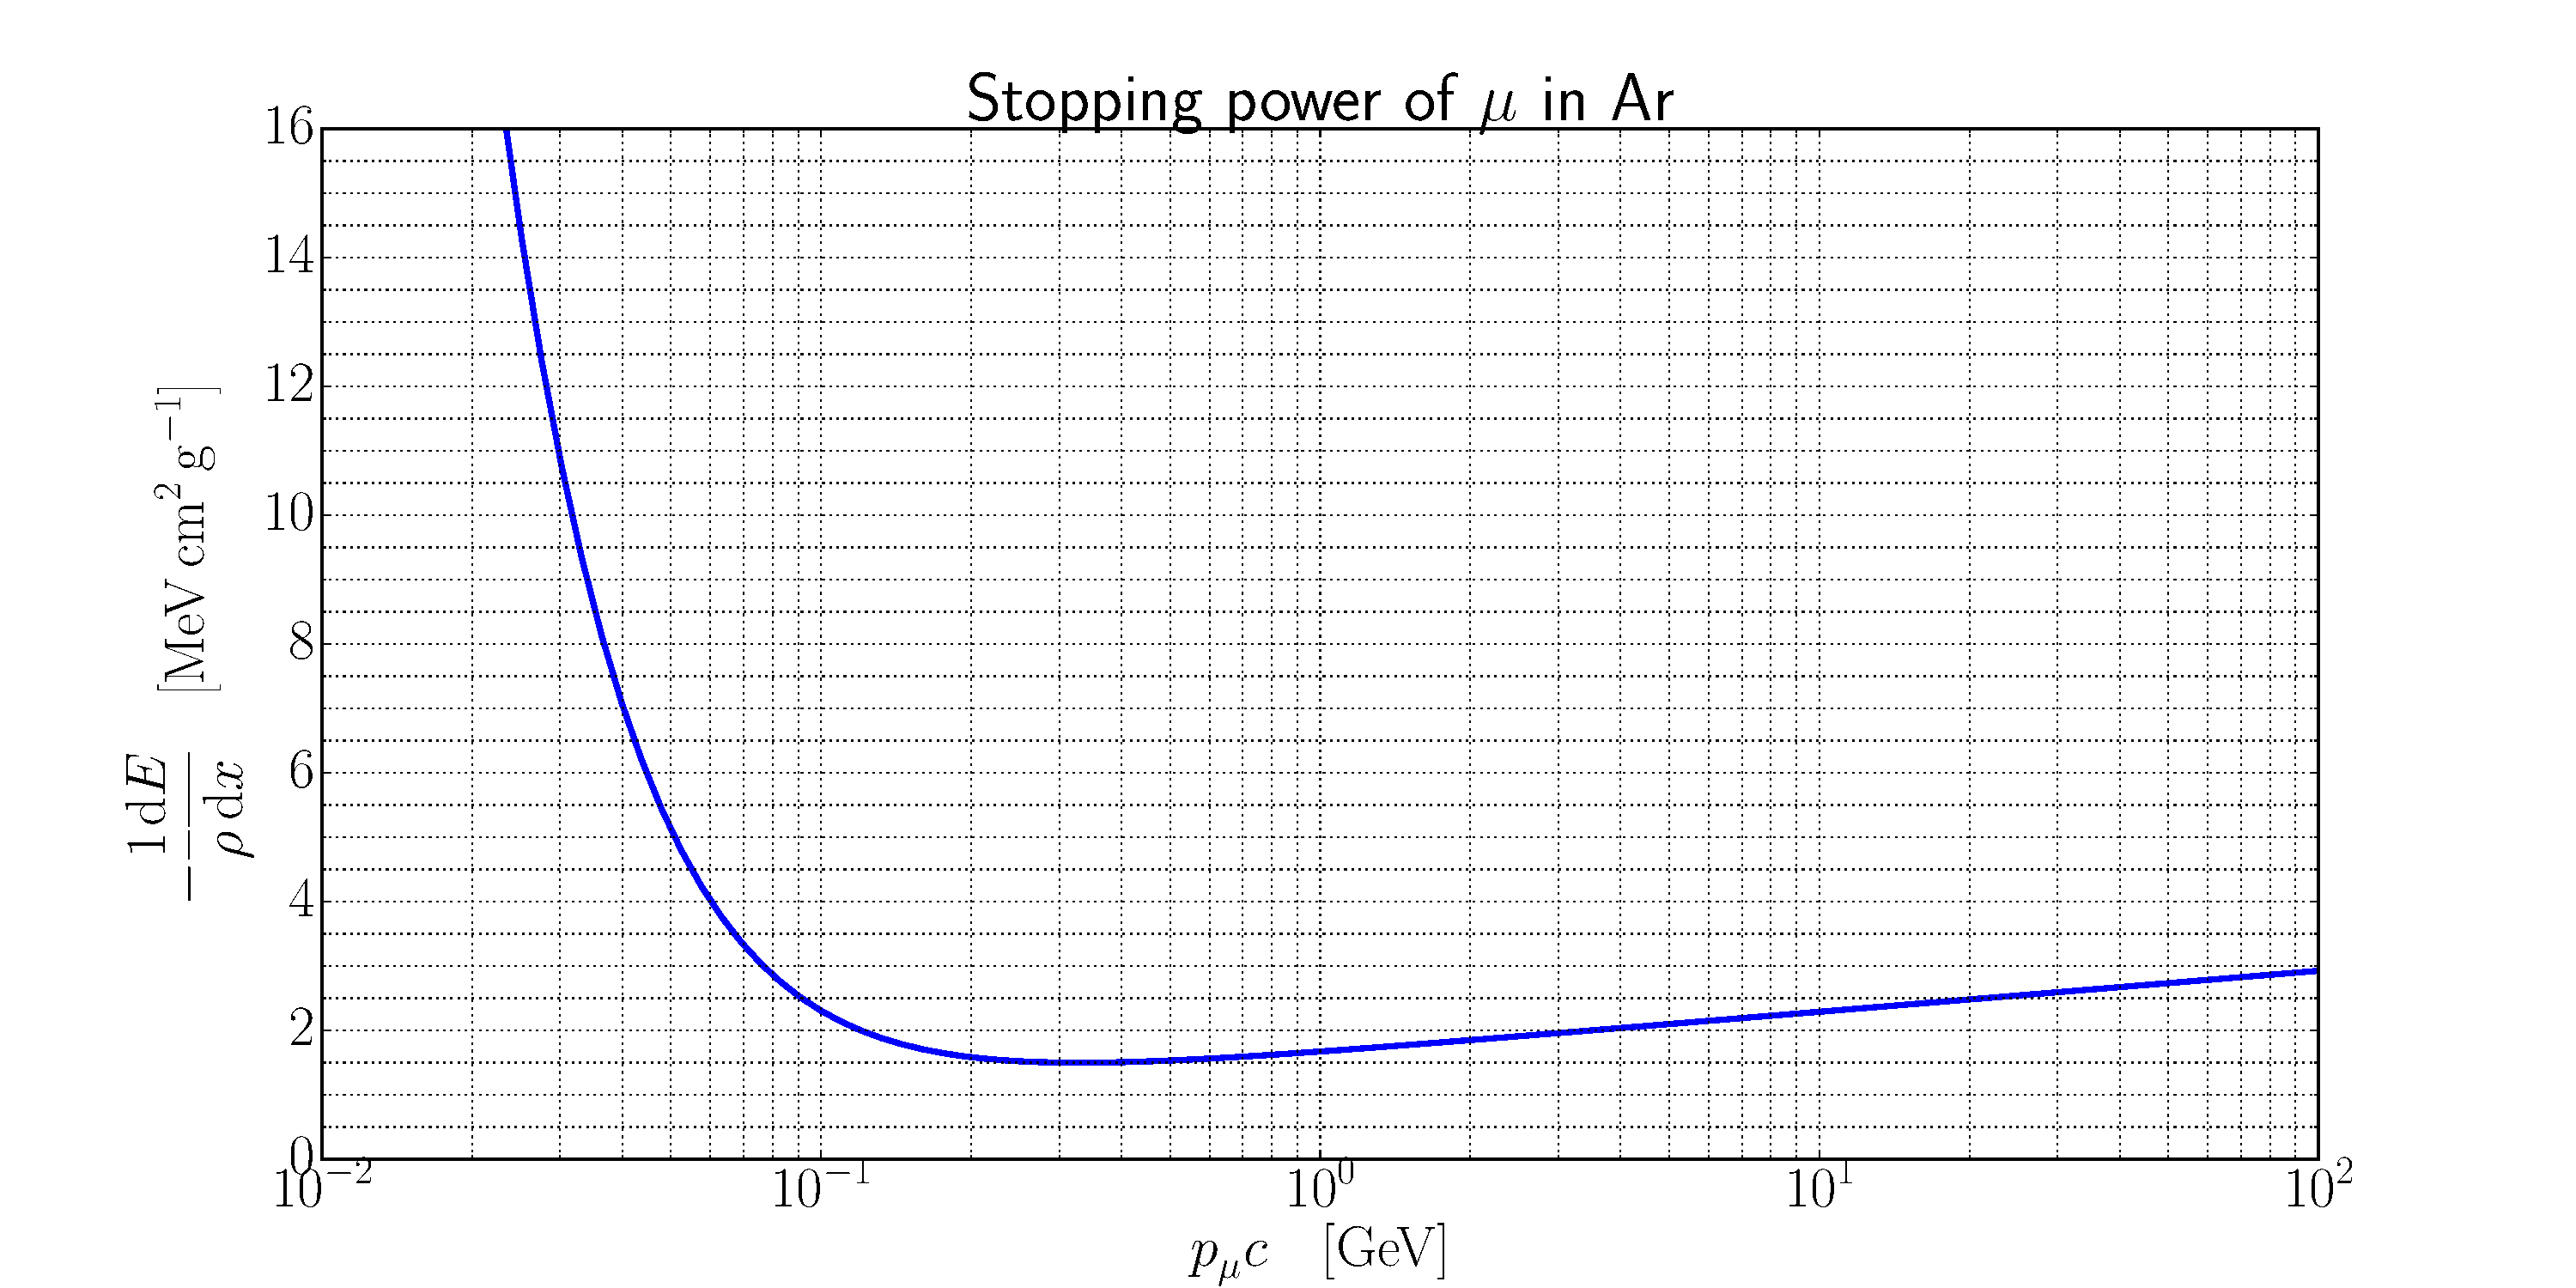
\includegraphics[width=\textwidth]{nu-detection/bethe_bloch}
	\caption[Stopping power]{%
		Bethe-Bloch stopping power of \Pgm in \ce{Ar}.
	}
	\label{fig:nu-detection_bethe-bloch}
\end{figure}

Figure~\ref{fig:nu-detection_bethe-bloch} shows the mass stopping power of muons in argon neglecting the $\frac{\delta}{2}$ term.
As can be seen, there is a broad minimum which is characteristic of the Bethe-Bloch formula.
Particles in this momentum range are called \glspl{mip}.
They are important for detectors because this energy loss is a measure for the required energy resolution of a detector.
As mentioned above, the mass stopping power only loosely depends on the absorber material and therefore, its minimum is
\begin{IEEEeqnarray}{rCl}
	\eval{- \frac{1}{\rho} \dv{E}{x}}_{\m{min}} & \approx & \SI{2}{\mega\electronvolt\centi\meter\squared\per\gram}
\end{IEEEeqnarray}
for singly charged incident particles on most (light) absorbers.
To the left of the minimum is the \emph{Bragg peak} which is especially important for radiation therapy with heavy charged particles (e.g.\ protons).
The Bragg peak falls off with a strong $\frac{1}{\beta ^ 2}$ dependence.
After the minimum, the stopping power rises again with a logarithmic dependence on $\beta$ and the mean excitation energy of the absorber $I$.
The reason for this so called \emph{logarithmic rise} is the extension of the transverse electric field of the incident particle in the relativistic regime.
Due to increasing shielding of the transverse electric field by the shell electrons of the absorber materials, taken into account by the $\frac{\delta}{2}$ term, the rise is only asymptotic.
For electrons and positrons, Equation~\eqref{eq:nu-detection_bethe-bloch} does not hold because their mass is equal to the mass of the atomic electrons of the absorber.
The stopping power changes further for electrons because the incident particle cannot be distinguished form its collision partner in that case.
On the other hand, a positron will be annihilated upon stop by an electron which needs to be taken into account as well.
The equivalent of Equation~\eqref{eq:nu-detection_bethe-bloch} for \Pepm can be found in~\cite{grupen}.

At high velocities further effects come into play.
\emph{Bremsstrahlung} describes the radiation energy loss of a fast charged particle in the Coulomb field of the absorber nuclei.
It can be described by
\begin{IEEEeqnarray}{rCl}
	- \frac{1}{\rho}\dv{E}{x} & = & \frac{E}{X_{\m{0}}}
	\label{eq:nu-detection_bremsstrahlung}
\end{IEEEeqnarray}
where
\begin{IEEEeqnarray}{rCl}
	X_{\m{0}} & = & \frac{A}{4 \alpha N_A Z \qty(Z + 1) \qty(\frac{1}{4 \pi \varepsilon_{\m{0}}} \frac{\si{\elementarycharge} ^ 2}{m c ^ 2}) ^ 2 \ln(183 Z ^ {- \frac{1}{3}})}
	\label{eq:nu-detection_radiationlength}
\end{IEEEeqnarray}
is the \emph{radiation length} of the absorber material using
\begin{description}
	\item[$\alpha$] $\approx \frac{1}{137}$ the fine-structure constant and
	\item[$m$] the mass of the incident particle.
\end{description}
Again, the energy loss is proportional to the density of the absorber and for convenience, divided by the latter.
Bremsstrahlung is emitted in interactions of the incident particle with the absorber nuclei ($\propto Z ^ 2$) as well as with the atomic electrons of the absorber ($\propto Z$).
By neglecting the latter, one obtains the important relation
\begin{IEEEeqnarray}{rCl}
	X_{\m{0}} ^ {- 1} & \propto & Z ^ 2
\end{IEEEeqnarray}
as opposed to the $\propto Z$ dependence of the Bethe-Bloch formula.
Equation~\eqref{eq:nu-detection_bremsstrahlung} also holds for electrons as long as $E \gg \frac{m_{\Pe} c ^ 2}{\alpha Z ^ {\frac{1}{3}}}$.
Furthermore, looking at the dependence on the mass of the incident particle, one finds
\begin{IEEEeqnarray}{rCl}
	X_{\m{0}} & \propto & m ^ 2
\end{IEEEeqnarray}
using Equation~\eqref{eq:nu-detection_radiationlength}.
Therefore, the radiation length of an absorber material is usually given for electrons and the relation
\begin{IEEEeqnarray}{rCl}
	X_{\m{0}} & = & X_{\m{0}}^{\Pe} \frac{m ^ 2}{m_{\Pe} ^ 2}
\end{IEEEeqnarray}
can be used to get the radiation length for any charged particle of mass $m$.
Radiation losses play a significant role only at energies much higher than the energy of \glspl{mip}.
Using Equations~\eqref{eq:nu-detection_bethe-bloch} and~\eqref{eq:nu-detection_bremsstrahlung}, one can define a \emph{critical energy} $E_{\m{c}}$ by
\begin{IEEEeqnarray}{rCl}
	\eval{\dv{E}{x}_{\m{ion}}}_{E_{\m{c}}} & = & \eval{\dv{E}{x}_{\m{brems}}}_{E_{\m{c}}}
	\label{eq:nu-detection_ec}
\end{IEEEeqnarray}
at which radiation losses take over from ionisation losses.
Similar to the radiation length, the critical energy is proportional to $m ^ 2$.
Thus, it is most important for electrons while for other particles it becomes significant only at very high energies.
If we take the example of an iron absorber again for instance, we get $E_c^{\Pe} = \SI{20.7}{\mega\electronvolt}$ and $E_c^{\Pgm} = \SI{890}{\giga\electronvolt}$.

At high energies, there are additional types of radiation loss taking place, for instance direct electron-pair production and photonuclear interactions.
They shall not be described here.
Instead, only their $\propto E$ relation similar to bremsstrahlung losses shall be mentioned.
A description of those effects can be found in~\cite{grupen}.

In addition to the processes described above, charged particles traversing matter also undergo scattering in the Coulomb field of the nuclei of the traversed medium.
Accordingly, this process is called \emph{\gls{mcs}}.
The \gls{rms} of the \emph{scattering-angle distribution}
\begin{IEEEeqnarray}{rCl}
	\Theta_{\m{\glsentryshort{rms}}} & = & \frac{\SI{13.6}{\mega\electronvolt}}{\beta c p} z \sqrt{\frac{2 x}{X_{\m{0}}}} \qty[1 + 0.038 \ln(\frac{x}{X_{\m{0}}})]
	\label{eq:nu-detection_highland}
\end{IEEEeqnarray}
is defined by the momentum $p$, velocity $\beta c$ and charge $z$ of the scattered particle, and the thickness of the scattering medium $\frac{x}{X_{\m{0}}}$ in radiation lengths.
The distinct momentum dependence of this so-called \emph{Highland formula} can be used to reconstruct the momentum of the incident particle provided the angular resolution of the detector is fine enough.

Concerning the interactions of charged particles with matter, there is one important note regarding detectors.
While charge produced in interactions (i.e.\ ionisation) can be detected directly, light (i.e.\ excitation photons and photon radiation) first needs to be converted to charge to be detected.

The three most important interactions converting photons to charge are the \emph{photoelectric effect}, \emph{Compton Scattering}, and \emph{pair production}.
All of them have in common that they attenuate photon beams exponentially according to
\begin{IEEEeqnarray}{rCl}
	I & = & I_0 e ^ {- \mu x}
\end{IEEEeqnarray}
where $I_0$ and $I$ is the intensity before and after passing the absorber, respectively.
The thickness of the absorber is given by $x$ and
\begin{IEEEeqnarray}{rCl}
	\mu & = & \frac{N_A}{A} \sum_i \sigma_i
	\label{eq:nu-detection_mass-att-coeff}
\end{IEEEeqnarray}
is the \emph{mass attenuation coefficient} defined by the sum of the cross-sections $\sigma_i$ of the different interaction processes.

At low energies (ionisation energy $\le E_{\Pgg} \le \SI{100}{\kilo\electronvolt}$), photons primarily undergo conversion to charge by the photoelectric effect.
The photon is absorbed by an atom of the absorber which in turn is ionised and thus ejects one of its shell electrons.
The cross-section is given by
\begin{IEEEeqnarray}{rCl}
	\sigma_{\m{photo}} & = & \qty(\frac{32}{\epsilon ^ 7}) ^ \frac{1}{2} \alpha ^ 4 Z ^ 5 \sigma_{\m{Th}}^{\Pe}
\end{IEEEeqnarray}
where
\begin{description}
	\item[$\epsilon = \frac{E_{\Pgg}}{m_{\Pe} c ^ 2}$] is the reduced photon energy and
	\item[$\sigma_{\m{Th}}^{\Pe} = \frac{8}{3} \pi r_{\Pe} ^ 2 = \SI{6.65e-25}{\centi\meter\squared}$] is the \emph{Thomson cross-section} for elastic scattering of photons on electrons.
\end{description}

For energies $\approx \SI{1}{\mega\electronvolt}$, Compton scattering dominates the interaction of photons with matter.
Thereby, the photon is not absorbed by the atom but just scatters off one of its shell electrons with the cross-section
\begin{IEEEeqnarray}{rCl}
	\sigma_{\m{c}} & = & 2 \pi r_{\Pe} ^ 2 Z \left\{\qty[\frac{1 + \epsilon}{\epsilon ^ 2}] \qty[\frac{2 \qty(1 + \epsilon)}{1 + 2 \epsilon} - \frac{1}{\epsilon} \ln(1 + 2 \epsilon)]\right.\\
	& & \left. + \frac{1}{2 \epsilon} \ln(1 + 2 \epsilon) - \frac{1 + 3 \epsilon}{\qty(1 + 2 \epsilon) ^ 2}\right\}
\end{IEEEeqnarray}
obtained from the Klein-Nishina formula.
As only part of the photon's energy is absorbed while the rest is scattered, it makes sense to divide this cross -section into a scattering cross-section
\begin{IEEEeqnarray}{rCl}
	\sigma_{\m{cs}} & = & \frac{E_{\Pgg}'}{E_{\Pgg}}
\end{IEEEeqnarray}
and an absorption cross-section
\begin{IEEEeqnarray}{rCl}
	\sigma_{\m{ca}} & = & \sigma_{\m{c}} - \sigma_{\m{cs}}
	\label{eq:nu-detection_sigma-compton}
\end{IEEEeqnarray}
where $E_{\Pgg}$ and $E_{\Pgg}'$ is the energy of the photon before and after scattering, respectively.

At $E_{\Pgg} \ge 2 m_{\Pe} c ^ 2$, photons are capable of producing pairs of \Pep\Pem.
Because of momentum conservation, this process can only happen in the Coulomb field of a so called spectator particle.
As pair-production in the field of an electron is strongly suppressed, the spectator is usually a nucleus of the absorber material.
Therefore, the cross-section of pair-production depends on the shielding of the Coulomb field by the shell electrons and thus on the proximity to the nucleus.
Eventually, this results in an energy dependence.
For $1 \ll \epsilon < \frac{1}{\alpha Z ^ {\frac{1}{3}}}$, the cross-section is given by
\begin{IEEEeqnarray}{rCl}
	\sigma_{\m{pair}} & = & 4 \alpha r_{\Pe} ^ 2 Z ^ 2 \qty(\frac{7}{9} \ln 2 \epsilon - \frac{109}{54})
\end{IEEEeqnarray}
and for $\epsilon \gg \frac{1}{\alpha Z ^ {\frac{1}{3}}}$, the cross-section is
\begin{IEEEeqnarray}{rCl}
	\sigma_{\m{pair}} & = & 4 \alpha r_{\Pe} ^ 2 Z ^ 2 \qty[\frac{7}{9} \ln(\frac{183}{Z ^ {\frac{1}{3}}}) - \frac{1}{54}] \qq*{.}
\end{IEEEeqnarray}

As mentioned above, for Compton scattering, two different cross-sections are defined, $\sigma_{\m{cs}}$ for the scattered energy and $\sigma_{\m{ca}}$ for the absorbed energy.
Consequentially, there are also different definitions of the coefficient $\mu$ in Equation~\eqref{eq:nu-detection_mass-att-coeff}.
Replacing the total Compton cross-section $\sigma_{\m{c}}$ by $\sigma_{\m{ca}}$ from Equation~\eqref{eq:nu-detection_sigma-compton}, one gets the \emph{mass absorption coefficient} $\mu_{\m{a}}$, only taking into account photon absorption processes.
While $\mu$ is more precisely called the \emph{total mass attenuation coefficient}.

An interesting effect takes place for \Pepm traversing material at energies higher than the critical energy $E_{\m{c}}$ defined by Equation~\eqref{eq:nu-detection_ec}.
In this regime, the energy loss is dominated by bremsstrahlung for \Pepm and by pair production for photons.
This leads to an \emph{\gls{em} cascade} or \emph{shower} where \Pepm and \Pgg produce each other alternately in a self-sustaining process.
The mean free path of a photon before pair production
\begin{IEEEeqnarray}{rCl}
	\lambda_{\m{prod}} & = & \frac{9}{7}X_{\m{0}}
\end{IEEEeqnarray}
is very close to the mean free path of an \Pepm before bremsstrahlung, the radiation length $X_{\m{0}}$.
Therefore, the number of particles participating in the shower doubles roughly every radiation length resulting in an exponential growth.
This allows \gls{em} showers to be approximated by the following rather simple model.
When the average energy per paticle drops below the critical energy, ionisation losses begin to dominate over radiative losses for \Pepm and Compton and photoelectric effect over pair production for photons.
At this point, the shower reaches its maximum and
\begin{IEEEeqnarray}{rCl}
	t_{\m{max}}^{\m{EM}} & = & \frac{\ln(\frac{E}{E_{\m{c}}})}{\ln(2)}
\end{IEEEeqnarray}
is its longitudinal extent in radiation lengths.
The \emph{Molière radius}
\begin{IEEEeqnarray}{rCl}
	R_{\m{M}}^{\m{EM}} & = & \frac{\SI{21}{\mega\electronvolt}}{E_{\m{c}}} X_{\m{0}}
\end{IEEEeqnarray}
is the transversal extent of the shower divided by the the material density.
Both $t_{\m{max}}^{\m{EM}}$ and $R_{\m{M}}^{\m{EM}}$ are important benchmarks for the dimensioning of \gls{em} calorimeters.
Naturally, a photon in the energy range where pair production dominates will produce a shower as well.
On the other hand, also \Pgmpm can start \gls{em} cascades, if there energy is high enough to produce bremsstrahlung.

Similarly, hadrons interacting with matter via the strong force can produce cascades as well.
As opposed to the \gls{em} showers governed only by \Pepm and \Pgg, the hadronic process is much more complex because many different secondary particle can be involved.
Hadrons start to shower because they mainly interact inelastically with matter, producing secondary strongly interacting particles.
That is why the hadronic cross-section
\begin{IEEEeqnarray}{rCl}
	\sigma_{\m{total}} & = & \sigma_{\m{elastic}} + \sigma_{\m{inel}}
\end{IEEEeqnarray}
is usually split.
From $\sigma_{\m{inel}}$, one can derive the \emph{interaction length}
\begin{IEEEeqnarray}{rCl}
	\lambda_{\m{int}} & = & \frac{A}{N_{\m{A}} \rho \sigma_{\m{inel}}}
\end{IEEEeqnarray}
which describes the absorption of hadrons in matter according to
\begin{IEEEeqnarray}{rCl}
	N & = & N_{\m{0}} e ^ {- \frac{x}{\lambda_{\m{int}}}}
\end{IEEEeqnarray}
with the initial number of hadrons $N_{\m{0}}$ and number of hadrons $N$ after a distance $x$ of absorber material.
For absorbers with $Z \geq 6$, the interaction length is much larger than the radiation length $X_{\m{0}}$ meaning that hadronic calorimeters usually need to be much larger than their \gls{em} counterparts.
Experimental data shows that hadronic showers from a few \si{\giga\electronvolt} to a few \SI{100}{\giga\electronvolt} can be approximated by similar parameters as \gls{em} showers.
The shower maximum is reached at
\begin{IEEEeqnarray}{rCl}
	t_{\m{max}}^{\m{had}} & = & 0.2 \ln(\frac{E}{\si{\giga\electronvolt}}) + 0.7
\end{IEEEeqnarray}
interaction lengths.
From this, the longitudinal extent containing \SI{95}{\percent} is given by
\begin{IEEEeqnarray}{rCl}
	L_{0.95}^{\m{had}} & = & t_{\m{max}}^{\m{had}} + 2.5 \qty(\frac{E}{\si{\giga\electronvolt}}) ^ {0.13} \qc
	\label{eq:nu-detection_hardon-long}
\end{IEEEeqnarray}
in interaction lengths again.
Transversally, \SI{95}{\percent} of the shower are contained within a cylinder of radius
\begin{IEEEeqnarray}{rCl}
	R_{0.95}^{\m{had}} & \leq & \lambda_{\m{int}}
	\label{eq:nu-detection_hardon-trans}
\end{IEEEeqnarray}
which is independent of the energy and smaller for high-Z materials~\cite{hardon}.
	\chapter{The \glsentrylong{lartpc}}
\label{chap:lartpc}
\glsreset{lar}
\glsreset{tpc}

The \gls{tpc} is a derivative of Charpak's Multi-Wire Proportional Chamber (MWPC)\cite{mwpc} developed by Nygren in the late 1970s~\cite{nygrenTPC}.
Crossing charged particles ionise the detection medium which was gaseous in the original design.
To prevent the recombination of the ions and electrons, an electric field is applied.
In this field, the electrons drift towards a two-dimensional readout plane (an MWPC in the original design).
The charge readout is triggered by a scintillation light readout which also provides accurate timing of an event.
Using this, one can measure the time for the ionisation electrons to reach the readout plane.
As the drift speed of charged particles in the detection medium is constant and if it is known, the coordinate in drift direction can be calculated from the drift time.

While gaseous \glspl{tpc} already provide very accurate tracking, they have the disadvantage that the target mass and thus, the cross-section of the detection medium is quite low resulting in a low interaction rate.
Therefore, in 1977, Rubbia proposed to use \lar{} as a detection medium~\cite{lartpc}.
This requires a cryogenic detector while gaseous detectors can be operated at room temperature.


\section{\glsentrylong{lar} as a Detection Medium}
\label{sec:lartpc_lar}

For an efficient particle detection by a \gls{tpc}, several properties of the sensitive medium are of interest, such as ionisation and light yield, electron-ion pair recombination, dielectric strength, length scales of electromagnetic and hadronic interactions, density, transparency to its own scintillation light, and the boiling point.
\lar{} is quite unique as it has all the necessary properties while at the same time it is comparably cheap because it is readily available in the Earth's atmosphere.
A summary of its properties can be found in Table~\ref{tab:lartpc_larprop}.
Xenon for instance slightly surpasses argon in many aspects but is prohibitively expensive to build large detectors.
A boiling point of $\approx \SI{87}{\kelvin}$ raises the need for strong thermal insulation and a potent cooling system for \lar{}, though the requirements are far less stringent then for liquid helium.
This section will outline the most important \lar{} properties.

\begin{table}[htb]
	\centering
	\caption{Properties of \lar{} taken from~\cite{NobleGasDetectors} where not specified otherwise.}
	\label{tab:lartpc_larprop}
	\begin{tabu} to \textwidth {llSs}
		\toprule
		Property &									Symbol &				{Value} &	{Unit} \\
		\midrule
		Molar mass &								$\mu$ &					3.9948e1 &	\gram\per\mol \\
		Boiling point at \SI{1.01325e5}{\pascal} &	$T_{\m{S}}$ &			8.726e1 &	\kelvin \\
		Density at $T_{\m{S}}$ &					$\rho_{\m{S}}$ &		1.399e3 &	\kilo\gram\per\cubic\metre \\
		Dielectric constant~\cite{dielConst} &		$\varepsilon_{\m{r}}$ &	1.504 &		\\
		Required energy per electron-ion pair &		$W_{\m{i}}$ &			2.36e1 &	\electronvolt \\
		Required energy per photon &				$W_{\m{sc}}$ &			1.95e1 &	\electronvolt \\
		Fano factor &								$F$ &					1.07e-1 &	\\
		Electromagnetic radiation length &			$X_{\m{0}}$ &			1.4e-1 &	\metre \\
		Hadronic interaction length &				$\lambda_{\m{int}}$ &	8.37e-1 &	\metre \\
		Peak scintillation wavelength &				$\lambda_{\m{scint}}$ &	1.28e-7 &	\metre \\
		Scintillation attenuation length &			$\lambda_{\m{att}}$ &	6.6e-1 &	\metre \\
		Concentration in air by volume &			&						9.34e-1 &	\percent \\
		\bottomrule
	\end{tabu}
\end{table}

In order to register the ionisations tracks of charged particles in a \gls{tpc}, two processes are crucial: production and transportation of charge.
The charge production needs to be high enough to be detectable by the available electronics.
This is given by the energy required to produce an electron-ion pair $W_{\m{i}}$.
The $W_{\m{i}}$ value of \SI{23.6}{\electronvolt} for \lar{} is challenging but manageable with contemporary electronics as shown in Section~\ref{sec:lartpc_electronics}.
Naturally, this imposes a lower limit on detectable $\frac{\m{d}E}{\m{d}x}$.

Charge transport is mainly influenced by three processes: \emph{recombination}, \emph{diffusion}, and \emph{lifetime}.
The ultimate goal is to collect as much of the produced charge as possible.
Recombination is the main process opposing this.
While it can be partially mitigated by increasing the electric field, it cannot be eliminated completely.
Even if that was possible, it would not be beneficial because the scintillation light needed for the drift time measurement is partly produced by recombining electron-ion pairs.
The relation between the strength of the drift field and charge yield can be described by the \emph{box model}~\cite{box-model}.
It assumes that the ion-electron pairs are isolated and initially uniformly populate a box of a given size.
Furthermore, the diffusion of electrons and ions as well as the ion drift velocity (\num{1e5} times smaller than for electrons) are assumed to be negligible.
For a produced charge $Q_{\m{0}}$ and a collected charge $Q$, the collection ratio is given by
\begin{IEEEeqnarray}{rCl}
	\frac{Q}{Q_{\m{0}}} & = & \frac{1}{\xi} \ln(1 + \xi) \qc
	\label{eq:lartpc_lar-reco}
\end{IEEEeqnarray}
with a parameter $\xi$ depending on the drift field, electron mobility, initial number of ion-electron pairs, chosen size of the box and recombination coefficient.
Figure~\ref{fig:lartpc_box-model} shows a measurement by LHEP of the collected charge in an \SI{8}{\milli\metre} drift \lartpc{} for different drift field intensities and nitrogen concentrations.

\begin{figure}
	\centering
	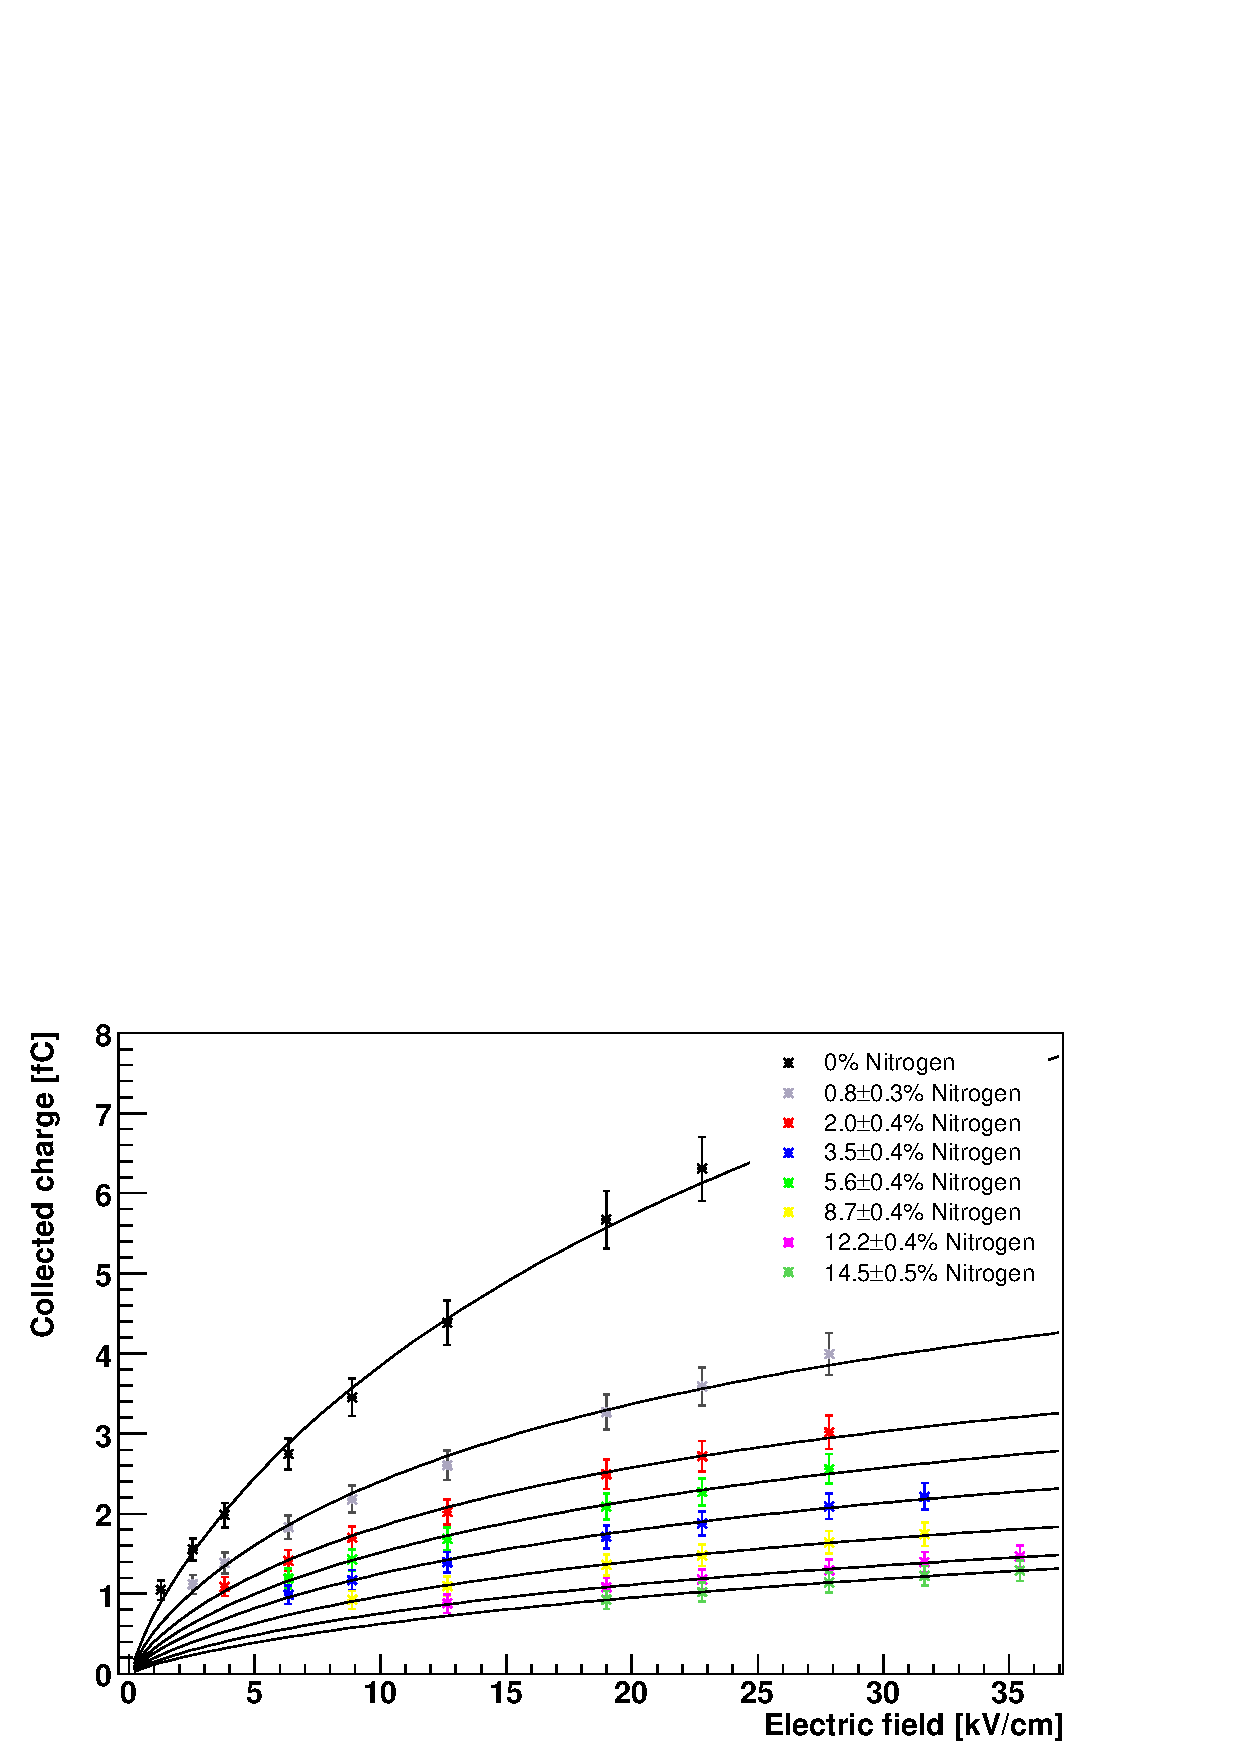
\includegraphics[viewport=14 5 511 351, clip, width=\textwidth]{lartpc/box-model}
	\caption{Collected charge in an \SI{8}{\milli\metre} drift \lartpc{} as a function of electric field, at various levels of nitrogen concentration.
	The lines represent box model fits.~\cite{grna-lhep}}
	\label{fig:lartpc_box-model}
\end{figure}

Due to thermal motion, ionisation charge clouds will start to diffuse over time.
The process is characterised by the diffusion coefficient $D$.
In the presence of a drift field, longitudinal ($D_{\m{L}}$) and transversal ($D_{\m{T}}$) components need to be treated separately.
The resulting smearing of the ionisation charge cloud after drift time $t$ is given by
\begin{IEEEeqnarray}{rCl}
	\sigma_{\m{L/T}} & = & \sqrt{2 D_{\m{L/T}} t}
	\label{eq:lartpc_lar-diff}
\end{IEEEeqnarray}
for longitudinal and transversal diffusion respectively.
Therefore, $D$ has the dimension of area per time.~\cite{lngDet}

A third process affecting charge transport is electron trapping by impurities, the probability of an electron becoming attached to an atom in the medium.
For the argon itself, this is highly unlikely because its outer electron shell is fully populated.
This is one of the reasons why (liquefied) noble gases are a prime choice for \glspl{tpc}.
Nevertheless, drifting electrons can be captured by impurities in the argon.
Oxygen is particularly bad due to its high electronegativity.
Impurities are therefore often measured in oxygen-equivalent concentration.
Finite purity gives rise to a finite lifetime of free electrons in the medium.
\begin{IEEEeqnarray}{rCl}
	N_{\Pe} \qty(t) & = & N_{\Pe} \qty(0) e ^ {- \frac{t}{\tau}}
	\label{eq:lartpc_lar-lifetime}
\end{IEEEeqnarray}
is the charge left after a time $t$ for an electron lifetime $\tau$.

The velocity of the charge drifting in an electric field is related to the so-called mobility, $\mu$, by
\begin{IEEEeqnarray}{rCl}
	\va{v} & = & \mu\qty(\va{E}) \va{E} \qc
\end{IEEEeqnarray}
where $\mu$ in general depends on the electric field.
This means, the higher the field is, the higher the charge velocity and thus, the lower the drift time.
One wants to keep drift times low for multiple reasons.
One of them are the aforementioned impurities.
They cause the charge to posses a finite lifetime following an exponential decay with time.
A consequence is that higher impurities can be partially compensated by a higher field.
In a beam experiment with a given beam timing, increasing the drift time will increase pile-up, i.e. the number of events simultaneously present in the detector.
Pile-up in turn, complicates event reconstruction.
On the other hand, the readout electronics need to be fast enough to guarantee the required spatial resolution in the drift coordinate which defines an upper limit for the drift velocity.
A reasonable value from a purity point of view is a drift time of $\order{\SI{1}{\milli\second}}$.
For a detector size of $\order{\SI{1}{\metre}}$, the required drift speed is $\order{\SI{1}{\milli\metre\per\micro\second}}$ which requires a field of $\order{\SI{1}{\kilo\volt\per\centi\metre}}$.

For detectors much larger than \SI{1}{\metre}, a drift field of \SI{1}{\kilo\volt\per\centi\metre} becomes challenging due to the required high cathode voltage.
Soon after entering \lartpc{} R\&D, the Bern group realised that the reported dielectric strength of \lar{} is much lower~\cite{breakdown_14} than measured by Swan et al.\ in 1960~\cite{swan1, swan2}.
It turned out, opposing the assumption of Swan et al., that the dielectric strength is not independent of the absolute dimensions of the electrodes.
This led to a very detailed study of breakdowns in \lar{} in the course of this thesis which is presented in Section~\ref{sec:studies_hv}.

\todo[inline, caption={LAr specs}]{Check:
\begin{itemize}
	\item General specs
	\item Electronegativity
	\item Ionisation
	\item Scintillation
	\item Recombination
	\item Diffusion
	\item Dielectric strength
	\item Single- and dual-phase?
	\item Citations (\cite{NobleGasDetectors})
\end{itemize}
}


\section{Electric Field Generation}
\label{sec:lartpc_efield}

For charge separation and drift, an electric field of $\order{\SI{1}{\kilo\volt\per\centi\metre}}$ is needed inside the fiducial volume of a \lartpc{}.
An easy way to achieve this is by means of field shaping rings fed by a resistive divider between cathode and anode.
The drawback is the need for a feedthrough capable of withstanding the full cathode voltage.
One alternative is to generate the \gls{hv} inside the cryostat, for instance using a Greinacher voltage multiplier circuit as the one used for the \AT{} experiment at LHEP at the University of Bern~\cite{AT}.
A Greinacher multiplier works by pumping up a cascade of capacitors and diodes using a high frequency source.
However, while the voltage generation itself worked well, this approach proved to be impractical because the high frequency voltage needed to charge the multiplier interfered with the readout and therefore had to be turned off during data-taking.
Recharging, in turn, caused a lot of detector down time.


\section{Charge Readout}
\label{sec:lartpc_charge-ro}

Classically, the charge readout of a \lartpc{} is done using wires with a diameter of $\order{\SI{.1}{\milli\metre}}$.
One wire plane delivers a 2D projection of the ionisation tracks in the detection medium.
This has two consequences:
\begin{enumerate}
	\item At least two parallel wire planes are needed to be able to reconstruct the 3D event topology.
	\item In theory, the higher the complexity of the event, the more planes would be required to be able to fully reconstruct it.
\end{enumerate}
Multiple wire planes can be realised by operating only the last one (in drift direction) in charge collection mode.
All the preceeding wire planes are biased in a such a way that they are transparent to the incoming charge but pick up an induction signal during the passage of the latter.
A typical number of wire planes for currently operational detectors is three, tilted at \ang{60} to each other.


\section{Light Readout}
\label{sec:lartpc_light-ro}

In order to calculate the distance the charge has drifted along the electric field (i.e.\ the space coordinate perpendicular to the readout plane), one needs to record the drift time.
The data acquisition can record the time of the arrival of the charge at the readout plane.
What is missing is the time of the charge production.
This can be acquired by registering the scintillation light produced alongside the ionisation of the detection medium.
Contemporary detector designs employ \glspl{pmt} for this purpose.
\glspl{pmt} are a well established technology with a high quantum efficiency and a fast response.

The light impinging upon a \gls{pmt} is converted to an electron by a photo cathode coated on the sensitive surface of the \gls{pmt}.
These photo cathodes have a limited absorption spectrum.
In particular, the scintillation light of \lar{} does not fall inside this spectrum for most photo cathodes.
That is why the vacuum UV scintillation light needs to be converted to the visible range where it can be efficiently detected by a \gls{pmt}.
A widespread wavelength-shifter capable of achieving this is TetraPhenyl Butadiene (TPB).
Therefore, a common setup consists of either coating the \gls{pmt}~\cite{icarus}, or a surface in front of it~\cite{uboone} with TPB.


\section{Electronics}
\label{sec:lartpc_electronics}

This section gives an overview of charge readout electronics from the physics perspective.
A more detailed review is given in Section~\ref{sec:studies_electronics}.
Using $W_{\m{i}}$, the energy required to produce one electron ion pair, from Section~\ref{sec:lartpc_lar} and assuming a MIP, one gets

\begin{IEEEeqnarray*}{rCl}
	\dv{Q}{x}	= \frac{\eval{\dv{E}{x}}_{\m{MIP}}}{W_{\m{i}}} \si{\elementarycharge}
			&	= & \frac{\SI{210}{\kilo\electronvolt\per\milli\metre}}{\SI{23.6}{\electronvolt}} \si{\elementarycharge}
				\approx \SI{8900}{\elementarycharge\per\milli\metre}
				\approx \SI{1.4}{\femto\coulomb\per\milli\metre}
\end{IEEEeqnarray*}

as a rough estimation for the charge yield.
This calculation does not incorporate recombination, diffusion and charge lifetime, meaning that in a real experiment the value will be even lower.
The result is that the readout electronics need to be capable of detecting $\order{\si{\femto\coulomb}}$ charges.

That is why the charge signal needs to be amplified before digitisation.
This is achieved by means of an integrating amplifier which also converts the charge to a voltage.
Early \lartpc{} designs used preamplifiers outside the cryostat at room temperature for this.
From a noise point of view though, it is beneficial to put the amplifiers inside the cryostat submerged in \lar{} for two reasons.
Firstly, the closer to the source the amplifier is located, the shorter the low-signal lines will be, resulting in less pick-up noise.
Secondly, the temperature-dependent Johnson-Nyquist noise of the amplifiers will be reduced at cryogenic temperatures.

For the same reasons it makes sense to operate the entire analogue signal chain at cryogenic temperatures.
This would also help to eliminate ground loops which can pick-up noise inductively or provoke self-oscillation of the analog signal circuitry.
On the other hand, in general it is not easy to operate a circuit at cryogenic temperatures.
Usually, a complete redesign of the circuit is necessary due to most components operating outside their guaranteed temperature range.
For some complex active components like the amplifiers and digitisers, even a redesign of the integrated circuit might be necessary.
On the other hand, placing the digitisers too close to the readout might result in elevated noise levels due to the digital clocks coupling into the analogue signal path.

The requirements on the electronics are given by the required sensitivity of the detector.
The necessary bit depth of the digitisers is given by the required dynamic range, i.e.\ the minimum and maximum amount of charge the readout needs to be able to register.
While the spatial resolution in the two coordinates parallel to the readout plane is given by the pitch of the electrodes, the accuracy of the third coordinate is given by the timing accuracy.
This in turn depends on three properties: the timing accuracy of the light readout, the sampling time of the digitisers and the peaking time of the preamplifiers.
Peaking time is the time needed until the output of the preamplifier reaches its maximum (peak) for a delta pulse input.


\section{Challenges of Future Detectors}
\label{sec:lartpc_challenges}

To accomplish the physics goals of future neutrino detectors, outlined in Chapter~\ref{chap:introduction}, much higher statistics than with today's experiments are necessary.
There are two obvious ways to do this: Increase the beam flux and detector size.
Scaling up a \lartpc{} brings several challenges, in particular for the drift \gls{hv} and wire readout planes.

At the same drift field, the cathode voltage scales with the size of the detector in drift direction.
This in turn increases the required distance of the cathode from all grounded parts.
Where the cathode is close to the \lar{} vessel, this inevitably leads to more dead volume that cannot be used for particle detection.
\gls{hv} problems are worsened by the fact that an increased drift distance also means an increased drift time at the same field.
This can either be compensated by increasing the charge lifetime and thus the \lar{} purity accordingly or by increasing the drift speed and thus the drift field.
In summary, at the same \lar{} purity, the cathode voltage scales more than linearly with detector size in drift direction.

Further problems are associated with the classic wire readouts employed in \lartpc{}s, such as mechanical construction and event pile-up.
One of the mechanical requirements on a wire readout is that it should be as planar as possible.
Sagging wires caused by insufficient mechanic tension lead to distortions in spatial reconstruction.
For large detectors, possessing thousands of wires on a single frame, this becomes quite challenging.
Every wire that has a slight deviation in tension from its neighbours will start to sag.
This is worsened by the fact that the construction needs to withstand extreme temperature gradients during detector cool-down.

The second problem of wires, event pile-up is a consequence of the increased flux required for future experiments.
It is rooted in the way event reconstruction works for wires.
As mentioned above, effectively, wire planes do not produce real 3D event topologies but rather multiple 2D projections.
In order to achieve true 3D events, they need to be disentangled from the 2D projections.
If an event is complex enough, this cannot be done unambiguously with a limited number of 2D projections.
This problem is especially serious in case of a near detector.
The envisioned \dune{} near detector, for instance, is expected to see a total of \num{3.14e5} neutrino events per tonne of Ar for \SI{1e20}{POT} (protons on target).~\cite{dune2}
Scaling down this number to one beam spill (\SI{1e14}{POT})\footnote{Assuming a \SI{2}{\mega\watt} beam reaching \SI{2e21}{POT\per a} with a spill cycle of \SI{1.2}{\second} and \SI{66.7}{\percent} beam up-time.~\cite{dune2, dune4}} leads to $\approx \num{0.3}$ neutrino events.\todo{fix}
For a \SI{30}{\tonne} near detector, this would result in \num{9} neutrino events per beam spill excluding any additional cosmic-induced events.

On top of the event reconstruction problems, event pile-up also poses a challenge for trigger accuracy.
In a monolithic detector, the scintillation light produced alongside the ionisation charge scatters across a large volume triggering a big portion of the light readout system.
Thus, matching a scintillation flash to the corresponding charge to get the correct timing of the event is a non-trivial task.
	\chapter{Experimental Studies on \glsentrylong{hv}, Charge and Light Readout}
\label{chap:studies}

\glsreset{hv}

Chapter~\ref{chap:lartpc} gave an overview of the traditional \lartpc{} design and concluded with the challenges such a design will face in future experiments.
This chapter comprises several studies of these challenges and potential solutions.
First, an in-depth study of the dielectric strength of \lar{} and the implications on the drift \gls{hv} systems and \lartpc{} design in general are presented.
Then, the theory of a pixelated charge readout and the resulting requirements for new charge readout electronics are discussed.
Finally, a new light collection system base on cold \glspl{sipm} coupled with a light trap is introduced.


\section{Study of Electric Breakdowns in \glsentrylong{lar}}
\label{sec:studies_breakdown}

During the commissioning and operation of the \AT{} detector demonstrator~\cite{AT} at \gls{help} it was found that the dielectric strength of \lar{} was much lower~\cite{breakdown_14} than predicted by earlier studies~\cite{swan1, swan2}.
Subsequently, I conducted a detailed study of dielectric breakdowns in \lar{}, including high-speed footage, current-voltage characteristics, and optical spectrometry.
The results are presented in this section, they have been published in a paper~\cite{breakdown_16}, of which I am corresponding author.

\begin{figure}[htb]
	\centering	
	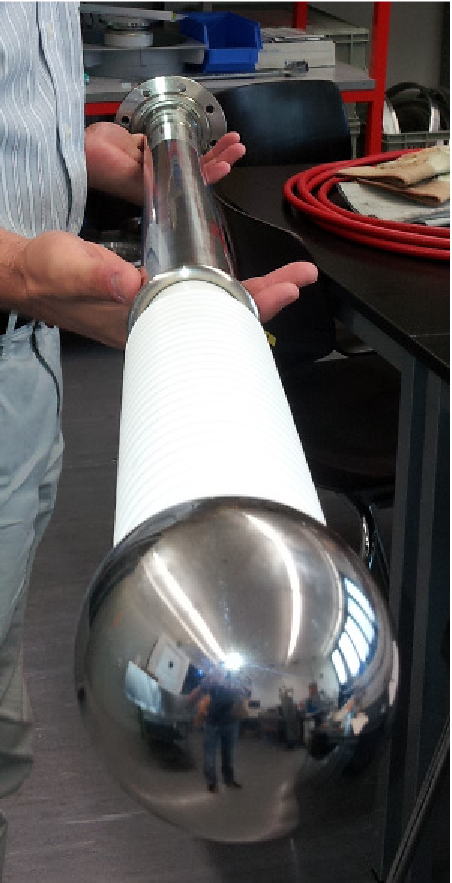
\includegraphics[width=0.265\textwidth]{hv/FT}
	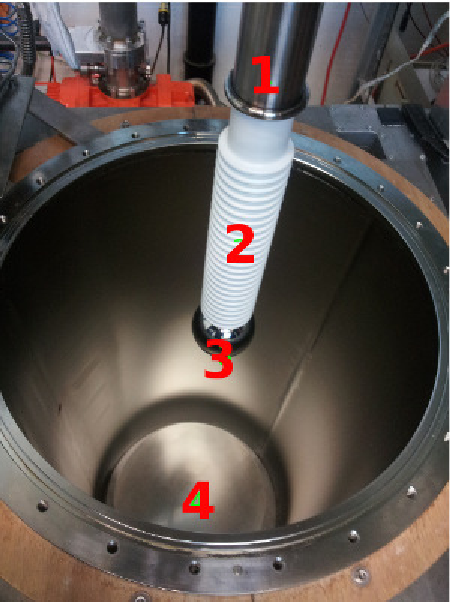
\includegraphics[width=0.39\textwidth]{hv/setup1_lowres}
	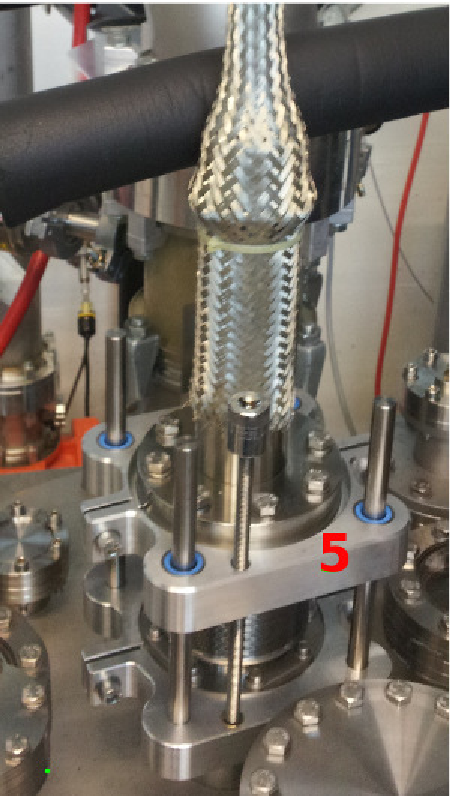
\includegraphics[width=0.295\textwidth]{hv/setup2_lowres}
	\caption[\glsentryshort{hv} test setup]{%
		Experimental setup used for the breakdown studies.
		Left: \acrshort{hv} feedthrough with spherical cathode.
		Middle: feedthrough before insertion into the cryostat.
		1.~ground shield; 2.~ribbed \acrshort{petc} dielectric; 3.~spherical cathode; 4.~anode plate sitting on a tripod on the grounded cryostat bottom; two of the tripod legs are insulated while the third one contains a \SI{50}{\ohm} shunt resistor.
		Right: linear translation unit used to set the cathode-anode gap width~(5).
	}
	\label{fig:hv_setup1}
\end{figure}

The setup used in this study is very similar to the one described in~\cite{breakdown_14} and is shown in Figure~\ref{fig:hv_setup1}.
A spherical cathode and a plane anode electrode form the discharge gap.
Three different diameters of the cathode sphere were tested: \SIlist{4; 5; 8}{\centi\metre}.
Two types of surface treatment were used in the cathode preparation, namely mechanical fine-polishing and electro-polishing.
For the anode mechanical fine-polishing was used for all measurements.
The anode-cathode gap width can be set in the range of \SIrange{0}{100}{\milli\metre} with a precision of \SI{0.3}{\milli\metre}.
An example of the field distribution in the setup is shown in Figure~\ref{fig:hv_efield}.
The field map was calculated using the COMSOL \gls{fem} package\footnote{\url{https://www.comsol.com}}.

\begin{figure}[htb]
	\centering	
	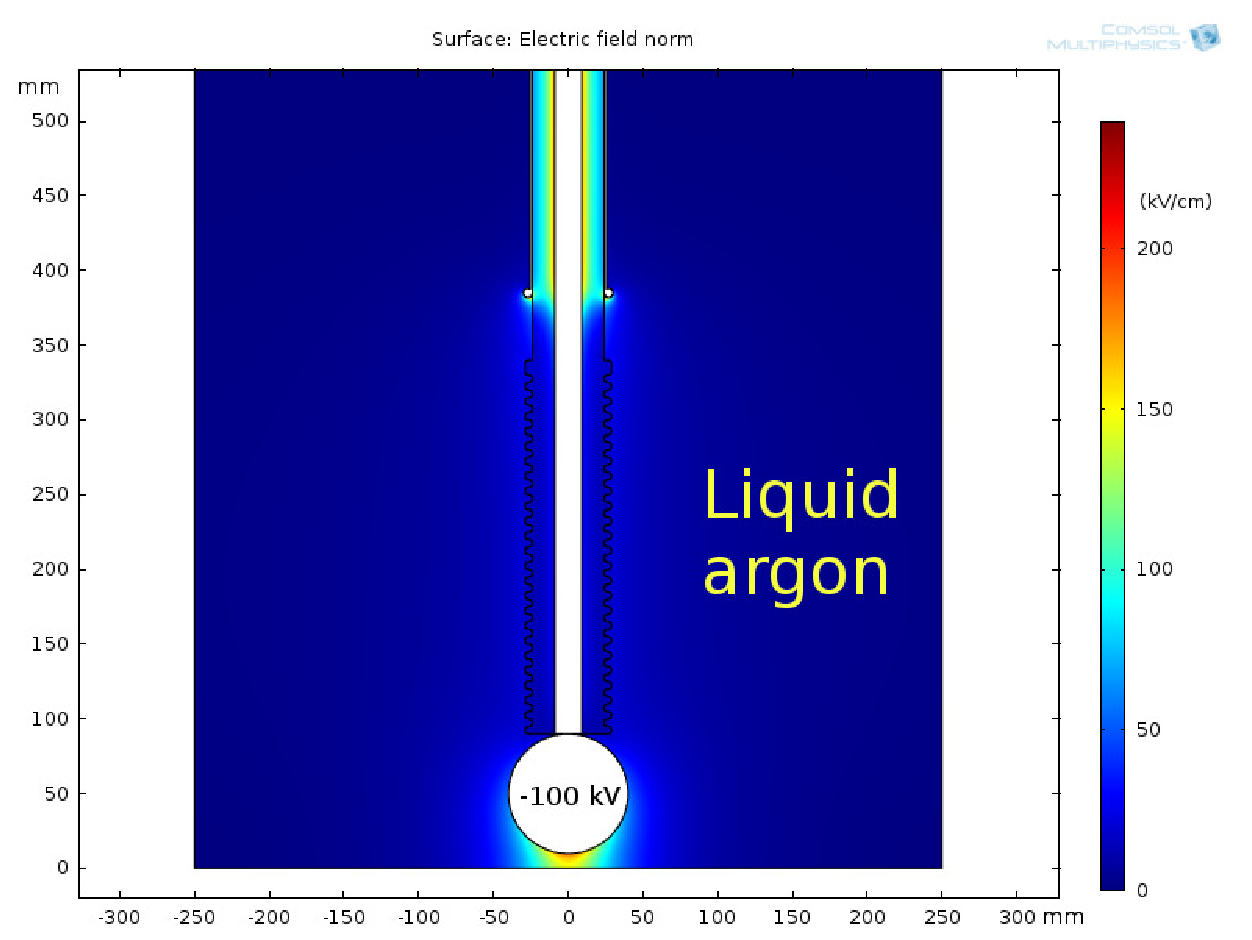
\includegraphics[width=\textwidth]{hv/EField}
	\caption[\glsentryshort{hv} test field map]{%
		Calculated electric field amplitude map for the test setup with \SI{-100}{\kilo\volt} at the cathode and a cathode-anode distance of \SI{1}{\centi\metre}.
	}
	\label{fig:hv_efield}
\end{figure}

The argon purity after filling was estimated with a small \gls{tpc} (according to the method described in~\cite{2photonAbs}) to be $\sim{\SI{1}{ppb}}$ of oxygen-equivalent impurity concentration.
More details on the setup can be found in~\cite{breakdown_14}.

The control circuit of the \emph{Spellman SL130PN150} \gls{hv} \gls{psu}~\cite{hv_psu} outputs two low voltages proportional to the voltage and the current at the output, respectively.
These voltages are recorded with a \emph{Tektronix DPO 3054} digital oscilloscope~\cite{hv_dpo} controlled by a LabVIEW\footnote{\url{https://www.ni.com/labview}} program.
The output polarity of the \gls{psu} can be switched by replacing the output \gls{hv} multiplier module.
To measure the discharge current a \SI{50}{\ohm} shunt resistor is placed between the anode plate and the vessel ground, which is connected to the ground return of the \gls{psu}.
The voltage drop across the shunt resistor is transmitted to the oscilloscope via a matched coaxial line.
Figure~\ref{fig:hv_scheme} shows the equivalent electric schematic of the setup. 
The voltage at the $V_{\m{mon}}$ output of the power supply corresponds to the \gls{psu} output voltage divided by a factor $K_{\m{V}}$; the voltage at $I_{\m{mon}}$ is related to the \gls{psu} output current.
However, according to the manufacturer of the \gls{psu} an accurate reconstruction of the output current for frequencies above \SI{100}{\hertz} is not possible because of a filtering circuit in the current control loop.
Therefore, only the voltage drop across the shunt resistor is used for the measurement of the discharge current.

\begin{figure}[htb]
	\centering
	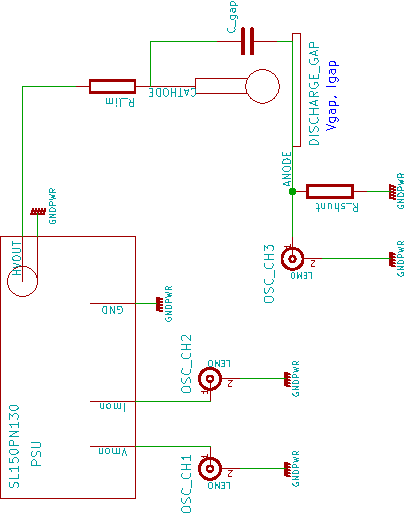
\includegraphics[width=0.7\textwidth]{hv/scheme}
	\caption[\glsentryshort{hv} test schematic]{%
		Electric schematic of the experimental setup.
		The oscilloscope is connected to the control circuit of the \acrshort{hv} power supply and to a shunt resistor on the ground return path.
		Discharge voltage and current can be derived from the recorded voltages.
	}
	\label{fig:hv_scheme}
\end{figure}

The oscilloscope is triggered by the channel connected to the shunt resistor.
The breakdown discharge current is composed of the output current of the \gls{psu} and the discharge current of the setup capacitance $C_{\m{gap}}$ as $I_{\m{gap}} = I_{\m{out}} + C_{\m{gap}}\frac{\m{d}V_{\m{gap}}}{\m{d}t}$.
To limit the \gls{psu} output current an additional resistor R$_{\m{lim}}$ is inserted into the \gls{hv} output circuit.
The measured values for the circuit parameters are summarised in Table~\ref{tab:hv_table1}.
The knowledge of these parameters allows to calculate the voltage across the gap during breakdown. 

\begin{table}[htb]
	\centering
	\caption[\glsentryshort{hv} test circuit parameters]{%
		Summary of the measured parameters of the test circuit.
	}
	\label{tab:hv_table1}
	\begin{tabu} to \textwidth {lSs}
		\toprule
		Parameter &			{Value} &	{Unit} \\
		\midrule
		$K_{\m{V}}$ & 		42.3e-6 &	\\
		$R_{\m{shunt}}$ &	50 &		\ohm \\
		$R_{\m{lim}}$ & 	200 &		\mega\ohm \\
		$C_{\m{gap}}$ & 	370 &		\pico\farad \\
		\bottomrule
	\end{tabu}
\end{table}

In addition, the setup is equipped with an \emph{AOS Technologies S-PRI} high-speed camera~\cite{hv_camera} to observe the development of the discharge.
The camera is capable of recording \num{700 x 400}~pixel \gls{rgb} images at \SI{1230}{fps}.
The camera comprises a frame ring buffer and is triggerable by an external \gls{ttl} pulse.
This allows a synchronous recording of the visual appearance of the discharge and its current-voltage characteristics.
The camera is triggered from the trigger output of the oscilloscope.
The luminous part of the discharge is analysed for each frame of the recorded sequence.

The camera is mounted above a \SI{5}{\centi\metre} diameter glass view port, located at the top flange of the cryostat, and is looking downward.
To observe a discharge from the side a glass mirror plate is installed at the edge of the cathode plane, located \SI{20}{\centi\metre} from the cathode in such a way as to not perturb the electric field in the discharge gap. 

Finally, a custom built optical spectrometer is used to analyse the light emission of the discharges.
The spectrometer is connected to an optical fibre entering the cryostat with its other end attached to the anode plate.
The fibre is aligned such that its end directly faces the discharge gap resulting in a high angular acceptance.
As will be shown later, the discharge emission spectra allow to better understand the processes at different stages of the discharge.
This is due to the fact that the emission spectra of excited neutral, singly-ionised, and multiply-ionised argon atoms lay in different regions of the visible spectrum.

The possibility of creating gas bubbles near the discharge gap is inhibited by keeping the pressure in the inner vessel at \SI{100}{\milli\bar} above atmospheric pressure, plus an additional \SI{100}{\milli\bar} due to the hydrostatic pressure.
The outer bath is opened to the atmosphere, thus keeping the inner vessel temperature constant and well below the boiling point.
No boiling was detected anywhere near the discharge gap region during the measurements.

\begin{figure}[htb]
	\centering	
	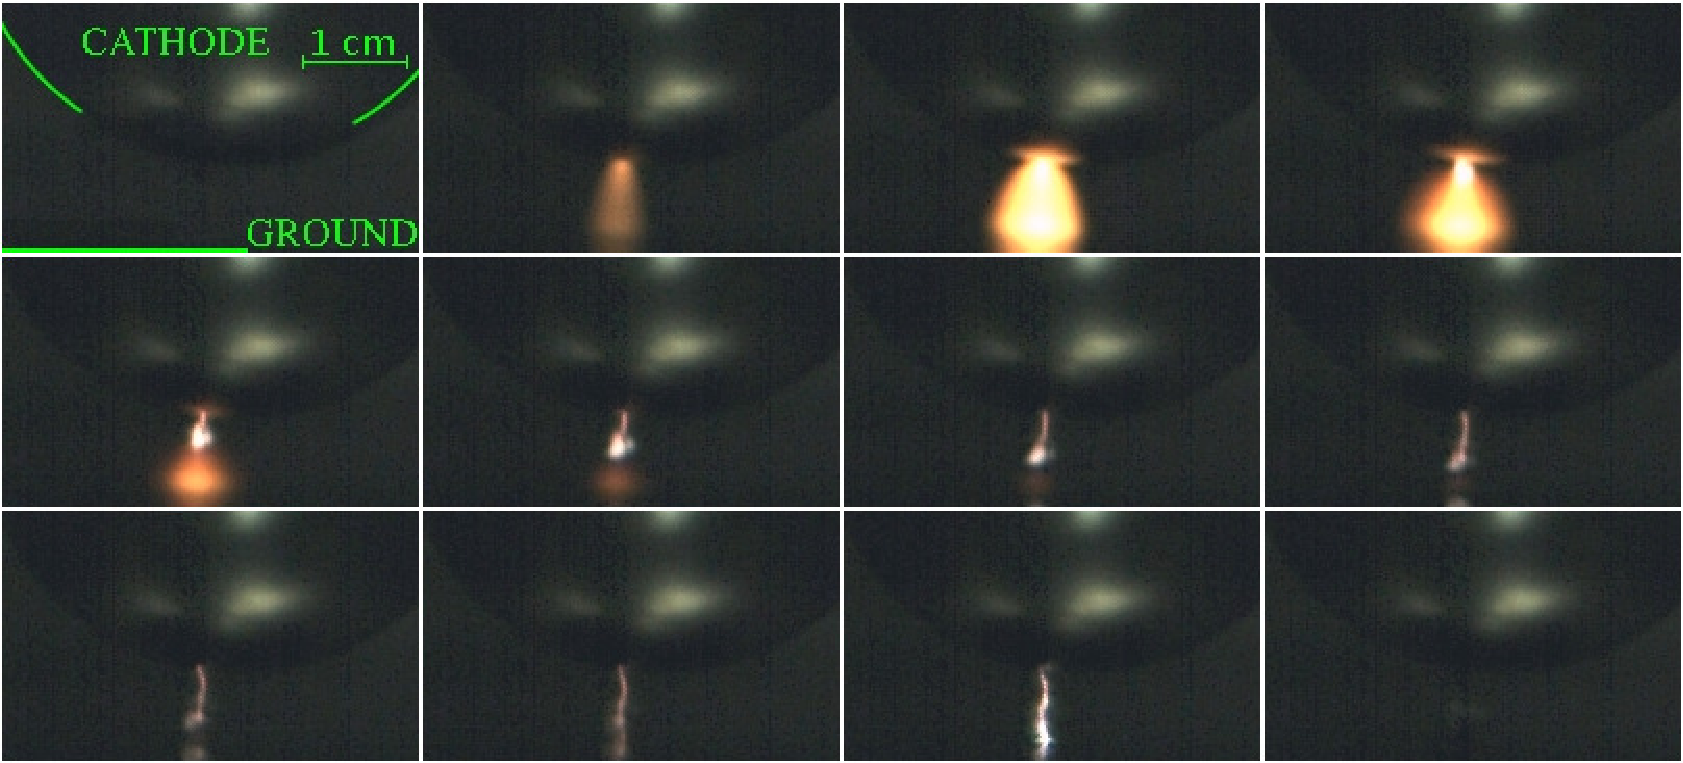
\includegraphics[width=\textwidth]{hv/montage}
	\caption[\glsentryshort{hv} test high-speed footage]{%
		Recorded camera image sequence for a breakdown from a \SI{5}{\centi\metre} diameter cathode at \SI{-100}{\kilo\volt} and \SI{8.8}{\milli\metre} apart from the anode plate.
		The sequence is taken at \SI{1250}{fps}, each frame takes \SI{0.8}{\milli\second}.
	}
	\label{fig:hv_images}
\end{figure}

In earlier measurements~\cite{breakdown_14} sporadic discharges were experienced across the ribs of the dielectric of the \gls{hv} feedthrough.
It was possible to suppress these discharges completely by rising the level of the \lar{} by about \SI{20}{\centi\metre}.
This improved the cooling of the feedthrough and reduced bubble production near the bottom of the feedthrough grounded shield, placed \SI{60}{\centi\metre} below the liquid surface. 

The measurement campaign comprised \num{5}~runs with a total of more than \num{5000}~measured discharges, for various sphere diameters, surface treatments, and polarities.
A summary is shown in Table~\ref{tab:hv_table2}.
A typical recorded camera image sequence for a breakdown from a \SI{5}{\centi\metre} diameter cathode at \SI{-100}{\kilo\volt} and \SI{8.0}{\milli\metre} apart from the anode plate is shown in Figure~\ref{fig:hv_images}.
The movie can be found as \emph{movie1.webm} in the ancillary files of~\cite{breakdown_16}\footnote{\url{https://arxiv.org/src/1512.05968v2/anc/movie1.webm}}.

\begin{table}[htb]
	\centering
	\caption[\glsentryshort{hv} test summary]{%
		Summary of the breakdown measurement runs.
	}
	\label{tab:hv_table2}
	\begin{tabu} to \textwidth {SSXXSSS}
		\toprule
		{Run} &	{$\varnothing_{\m{Sphere}} \qty[\si{\centi\metre}]$} &	Surface finish &	Sphere polarity &	{Events} &	{$d_{\m{Gap}} \qty[\si{\milli\metre}]$} &	{$V_{\m{Breakdown}} \qty[\si{\kilo\volt}]$} \\
		\midrule
		1   &	4 &														Mech.\ polished &	Cathode ($-$) &		1086 &		\numrange{0.5}{8.0} &						\numrange{3}{130} \\
		2   &	5 &														Mech.\ polished &	Cathode ($-$) &		900 &		\numrange{0.2}{12.0} &						\numrange{2}{130} \\
		3   &	8 &														Mech.\ polished &	Cathode ($-$) &		2434 &		\numrange{0.1}{70.0} &						\numrange{1}{130} \\
		4   &	5 &														Mech.\ polished &	Anode ($+$) &		102 &		\numrange{4.0}{5.0} &						\numrange{5}{114} \\
		5   &	5 &														Electro-polished &	Cathode ($-$) &		1141 &		\numrange{0.1}{10.0} &						\numrange{1}{130} \\
		\bottomrule
	\end{tabu}
\end{table}

\begin{figure}[p]
	\centering
	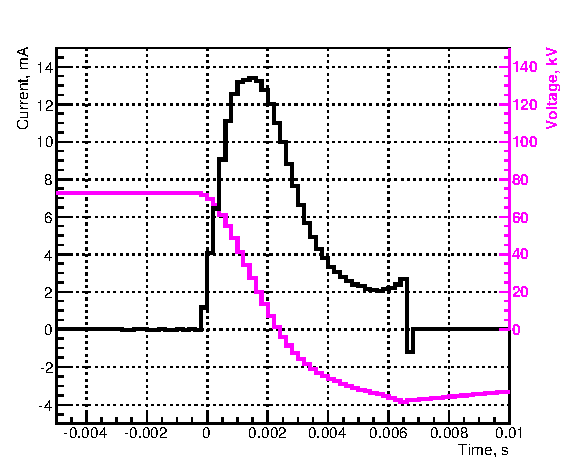
\includegraphics[height=0.43\textheight]{hv/IVuncorr}\\
	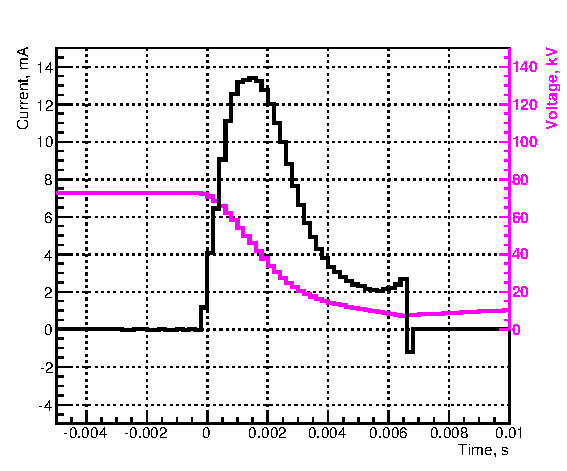
\includegraphics[height=0.43\textheight]{hv/IVcorr}
	\caption[\glsentryshort{hv} test current-voltage characteristics]{%
		Measured current through the gap (black) and voltage across the gap (magenta) for a typical breakdown at \SI{6.0}{\milli\metre} distance between a \SI{4}{\centi\metre} diameter cathode and the anode plate.
		The top plot shows the voltage obtained using the measured values of the protection resistor and the gap capacitance while the bottom plot uses the tuned values.
	}
	\label{fig:hv_iv}
\end{figure}

Figure~\ref{fig:hv_iv} shows the current and voltage features of a similar breakdown from a \SI{4}{\centi\metre} diameter cathode at \SI{6.0}{\milli\metre} from the anode plate.
The current was directly measured by observing the voltage drop across the shunt resistor while the voltage was obtained by integrating the current, taking into account the gap capacitance, protection resistor, and output voltage of the power supply.
Using the measured values of Table~\ref{tab:hv_table1} for capacitance and resistance results in a negative voltage at the end of most discharges.
This is an unphysical result, as can be seen in the top plot of Figure~\ref{fig:hv_iv}.
The behaviour may be attributed to poor knowledge of the effective values of the current-limiting resistor and the setup capacitance in the frequency domain of the discharge.
In order to better approximate these parameters they are tuned in such a way that the minimum voltage approaches zero for a maximum number of discharges.
The best result was achieved by lowering the resistance by a factor of \num{1.7} and increasing the capacitance by the same factor.
Interestingly, this result leaves the $RC$ characteristics of the system unchanged.
The bottom plot of Figure~\ref{fig:hv_iv} shows the result obtained by using the tuned values for capacitance and resistance.

Most of the discharges are localised in the area of high field concentration between the tip of the sphere and the anode plane.
However, in rare cases the discharge is initiated far from that region, sometimes at the side surface of the sphere.
An example of such a discharge is shown in Figure~\ref{fig:hv_side}, and the corresponding movie can be found as \emph{movie2.webm} in the ancillary files of~\cite{breakdown_16}\footnote{\url{https://arxiv.org/src/1512.05968v2/anc/movie2.webm}}.

\begin{figure}[htb]
	\centering	
	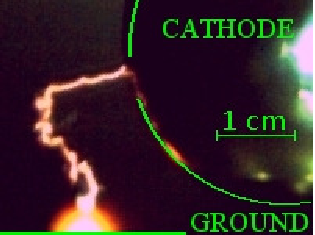
\includegraphics[width=.75\textwidth]{hv/sidespark}
	\caption[\glsentryshort{hv} test streamer image]{%
		An image of the streamer stage of the discharge, initiated at the side surface of a \SI{5}{\centi\metre} cathode sphere at \SI{-121.5}{\kilo\volt} and \SI{8.0}{\milli\metre} apart from the anode plate.
		The cone of electrons emitted from the streamer tip towards the anode (lower edge of the image) produces a bright orange luminescence in \acrshort{lar}.
	}
	\label{fig:hv_side}
\end{figure}

As was shown in \cite{FNAL-hv-paper, he-breakdown} experimental data on breakdowns in liquefied noble gases suggest the following dependence for the maximum breakdown field: $E_{\m{max}} = C A ^ p$, where $C$ is a material-dependent constant, $A$ is the stressed cathode area with an electric field intensity above \SI{90}{\percent} of its maximum, and $p \approx -0.25$.
Figure \ref{fig:hv_powerplot} combines data available in literature with data obtained from the measurements of this thesis and earlier measurements performed at \gls{help}.
Each data point is the mean value of all measurements of one run taken at the same gap distance and therefore stressed area.
The global best fit gives the following values for the parameters: $C = \num{139 +- 5}$ and $p = \num{-0.22 +- 0.01}$.
The statistical uncertainties represented by the error bars (smaller than the marker where not shown) are small compared to the unknown systematic uncertainties.
Indications for this are the high spread of the points around the fit line and the high reduced chi-square of \num{7283}.

\begin{figure}[htb]
	\centering
	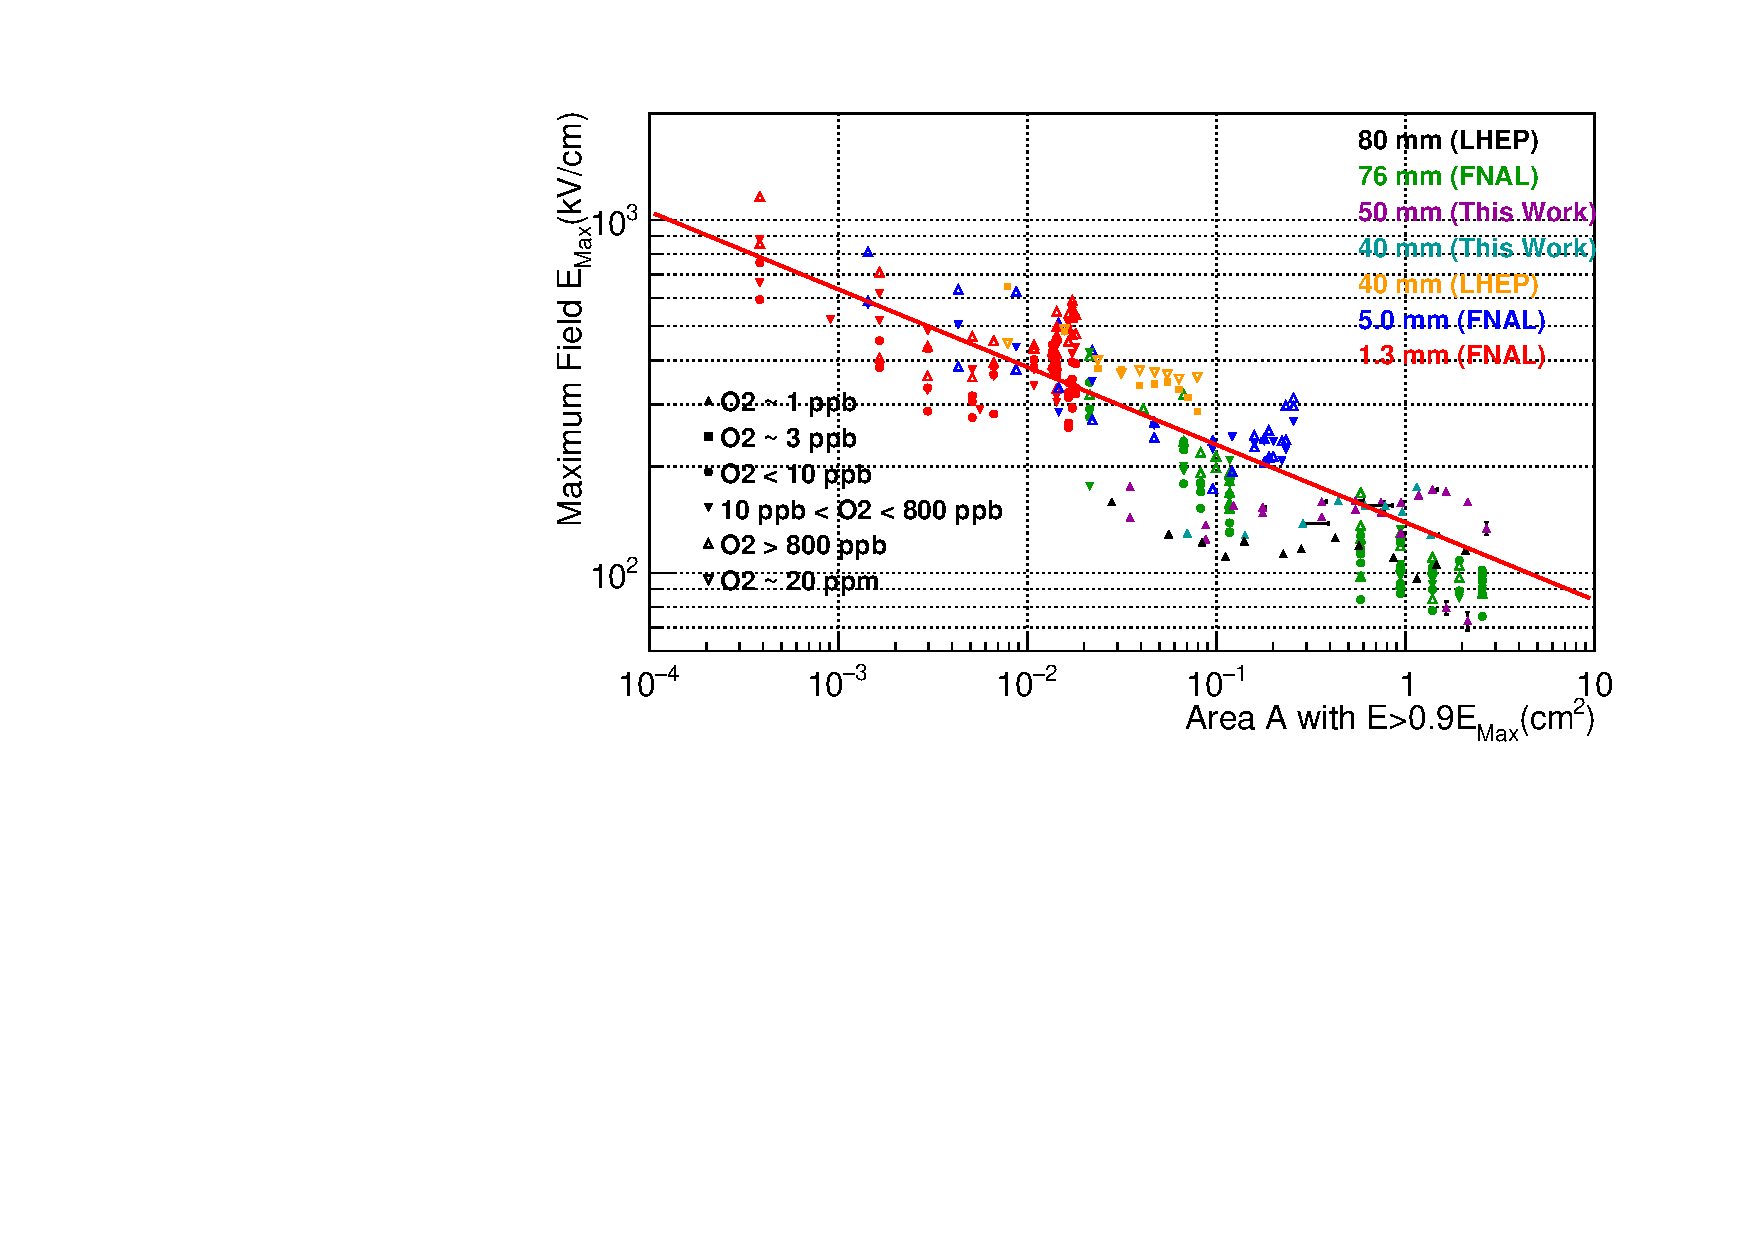
\includegraphics[width=\textwidth]{hv/Area90-1}
	\caption[\glsentryshort{hv} test breakdown field versus stressed cathode area]{%
		Breakdown field versus stressed cathode area.
		The stressed area $A$ is defined as the area with an electric field intensity greater than \SI{90}{\percent} of the maximum electric field intensity in the gap.
		The fit line represents the dependence $E_{max}=C A^p$ with $C = \num{139 +- 5}$ and $p = \num{-0.22 +- 0.01}$.
		The colours correspond to different cathode sphere diameters while the marker styles correspond to different oxygen-equivalent impurity concentrations.
		Data taken from \cite{FNAL-hv-paper}~(\acrshort{fail}), \cite{breakdown_14}~(\acrshort{help}), and \cite{breakdown_16}~(this work).
	}
	\label{fig:hv_powerplot}
\end{figure}

Figure~\ref{fig:hv_spectro} shows the recorded spectra of a typical event.
The spectra are integrated over \SI{1}{\milli\second} and approximately correspond to frames \num{3} (blue) and \num{8} (red) in Figure~\ref{fig:hv_images}.
Three phases of breakdown development can be distinguished from the observation of the emitted light spectra and discharge appearance.
The first phase starts with the field emission of electrons from a point of the cathode metal surface.
The emitted electrons drift towards the anode, ionising and exciting argon atoms.
Frames \num{2} and \num{3} of Figure \ref{fig:hv_images}, the broad current peak of the current in Figure~\ref{fig:hv_iv}, and the blue curve in Figure~\ref{fig:hv_spectro} show the development of the emission.
Evidence for the presence of ionisation comes from the analysis of the emission spectrum in the cone formed by drifting electrons.

\begin{figure}[htb]
	\centering
	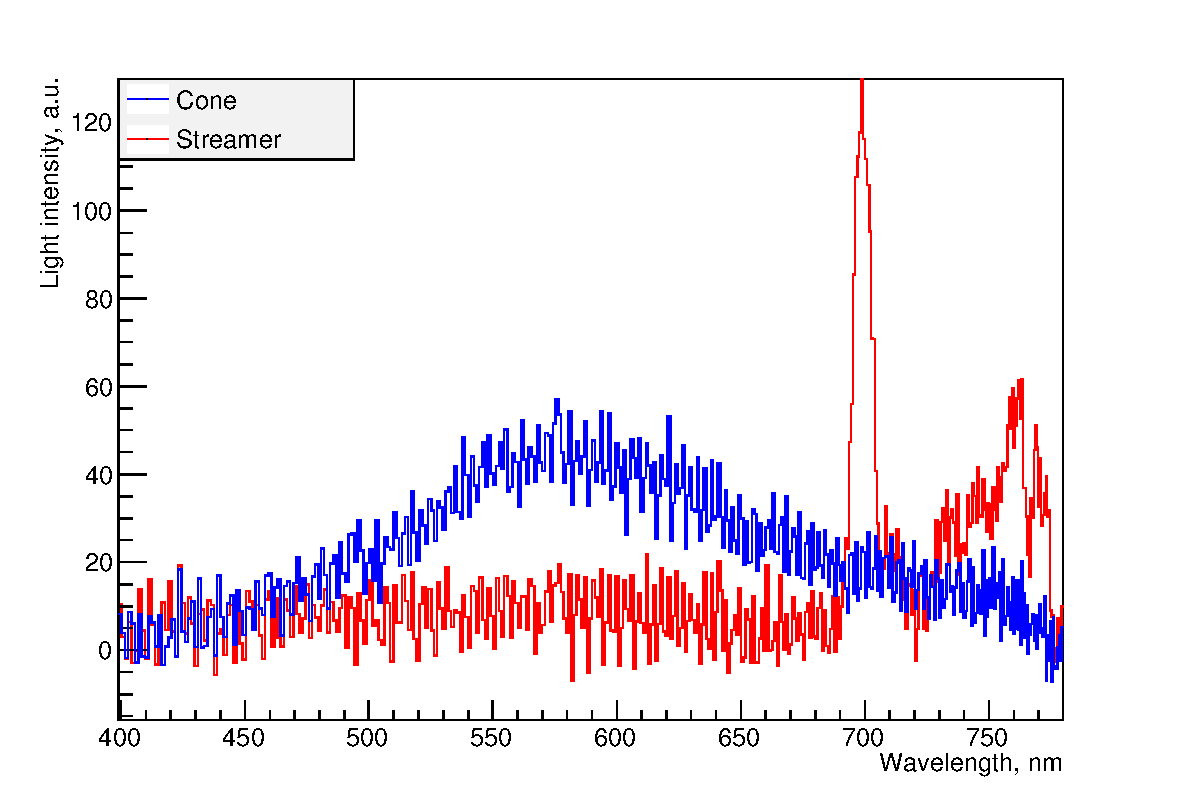
\includegraphics[width=\textwidth]{hv/spectro}
	\caption[\glsentryshort{hv} test field emission and streamer spectra]{%
		Spectra of the field emission cone (blue) and the streamer (red) for a breakdown from a \SI{4}{\centi\metre} diameter cathode at \SI{-56.2}{\kilo\volt} and \SI{3.0}{\milli\metre} apart from the anode plate.
		The spectra were integrated over a time of \SI{1}{\milli\second} with the spectrum of the streamer taken \SI{2}{\milli\second} after the spectrum of the cone.
		The blue curve is a broad continuum, similar to the scintillation spectrum of \acrshort{lar}, while the red curve features a distinct peak around \SI{700}{\nano\metre}, which is attributed the the 3p\textsuperscript{5}4p--3p\textsuperscript{5}4s transition of neutral argon gas.
	}
	\label{fig:hv_spectro}
\end{figure}

The emission of light by charged particles drifting in noble liquids under the influence of an electric field (electro-luminescence) gained great interest in the last years.
Recent studies in this field are well covered by~\cite{buzulutskov1, buzulutskov2, buzulutskov3} and references therein.
The red electro-luminescence, namely the peak around \SI{700}{\nano\metre} of the red curve in Figure~\ref{fig:hv_spectro}, produced by electrons drifting in argon gas is attributed to the 3p\textsuperscript{5}4p--3p\textsuperscript{5}4s transition of neutral argon~\cite{Boffard}.
The energy needed for the excitation of the electrons from the ground state to the 3p\textsuperscript{5}4p states in argon gas is \SIrange{12.9}{13.5}{\electronvolt}.
The ionisation potential of \lar{} is \SI{13.84}{\electronvolt}~\cite{2photonAbs}.
For the condensed state only the scintillation spectrum under ionisation by high-energy charged particles has been described in literature so far~\cite{Heindl}.
The electro-luminescence spectrum measured (blue curve in Figure~\ref{fig:hv_spectro}) exhibits a broad continuum, similar to the scintillation spectrum.
However, the centre value at about \SI{580}{\nano\metre} does not correspond to any of the electron transitions of neutral, singly-, or doubly-ionised argon atoms.
The nearest candidate for such an emission is the residual oxygen with its strong \SI{557.7}{\nano\metre} emission line.
However, if attributable to oxygen, this line has to be observed also at the later stages of the discharge, which does not take place in the measurements.

The broad width of the spectrum could be explained by smearing the energy levels into bands due to inter-atomic interactions in liquid and by the formation of exciton clusters~\cite{Bernstorff, Foerstel}.
If the energy band structure of excitons in \lar{} is continuous, as suggested by the scintillation spectrum, there might be a significant overlap of the band corresponding to the 3p\textsuperscript{5}4p atomic levels and the conduction band above \SI{13.84}{\electronvolt}.
The presence of an observable emission at about \SI{580}{\nano\metre}, in this case, is inevitably linked to a presence of ionised states.

Another signature of avalanche ionisation in this phase of the breakdown is the increase of the cone brightness as it develops from the cathode towards the anode.
Figure~\ref{fig:hv_conexpo} shows this increase together with the fitted avalanche multiplication parameter $\alpha = \SI{0.15 +- 0.03}{\per\milli\metre}$ for the following gap conditions: voltage $V = \SI{54.0}{\kilo\volt}$ across a gap of \SI{7.0}{\milli\metre}, cathode sphere diameter of \SI{4}{\centi\metre}, maximum field in the gap $E_{\m{max}} = \SI{96.1}{\kilo\volt\per\centi\metre}$, mean field in the gap $\expval{E} = \SI{87.0}{\kilo\volt\per\centi\metre}$.
To calculate the emission intensity the raw values of all pixels of the camera image in a row perpendicular to the cone direction were summed up.
The distance from the cathode can be derived from the known gap distance.
The given statistical uncertainty of $\alpha$ was obtained from the fit.
As only one measurement was taken, it is not possible to state anything about unknown systematic uncertainties (for instance the calibration of the camera).

\begin{figure}[htb]
	\centering
	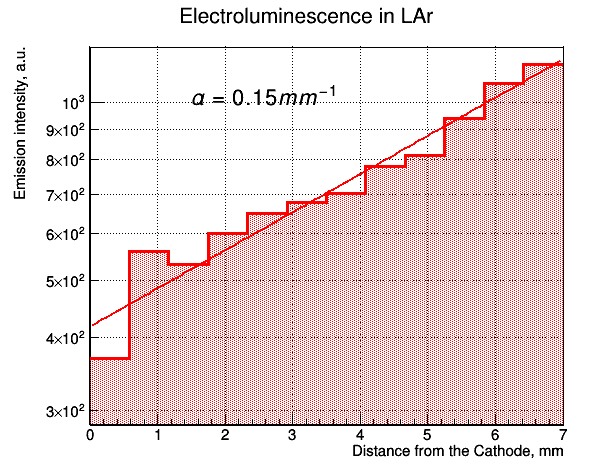
\includegraphics[width=\textwidth]{hv/ConeExpo.png}
	\caption[\glsentryshort{hv} test electro-luminescence brightness]{%
		Increasing brightness of the electro-luminescence cone as it develops towards the anode.
		The line represents the exponent with a fitted avalanche multiplication parameter $\alpha = \SI{0.15 +- 0.03}{\per\milli\metre}$ for gap conditions: voltage $V = \SI{54.0}{\kilo\volt}$ across a gap of \SI{7.0}{\milli\metre}, cathode sphere diameter of \SI{4}{\centi\metre}, maximum field in the gap $E_{\m{max}} = \SI{96.1}{\kilo\volt\per\centi\metre}$, mean field in the gap $\expval{E} = \SI{87.0}{\kilo\volt\per\centi\metre}$.
	}
	\label{fig:hv_conexpo}
\end{figure}

As already suggested in~\cite{breakdown_14}, positive ions produced in this process drift towards the cathode, raising the surface field and provoking a rapid increase of the field emission current to values $\sim{\SI{1}{\milli\ampere}}$.
Ions bombarding the cathode surface raise the local temperature and, after \SIrange{1}{2}{\milli\second}, the liquid near the initial discharge point transitions to a gas phase, forming a bubble.
Both the first and the second avalanche multiplication coefficients are a few orders of magnitude higher in gas than in liquid.
Therefore, the ionisation density in the gas bubble quickly rises along with the conductivity of the formed plasma.
This leads to a decrease of the electric field in the close vicinity of the field emission point and to the suppression of a further growth of the field emission current.
Accelerated electrons of the gas plasma hit the gas-liquid interface, forcing the bubble to elongate and grow.
In the region behind the head of the streamer the filament is collapsed to a diameter below \SI{200}{\micro\metre} (the spatial resolution of the camera) by surface tension and electro-striction forces.
This second phase of the discharge is characterised by the growth of the streamer-like filament in \lar{}.
In Figure~\ref{fig:hv_images} (frames \numrange{4}{10}) one can see the development of such a filament.
Unlike the electrons in the first phase the filament does not follow the electrostatic field lines but it rather rambles around their direction, being subject to thermodynamic fluctuations at the tip of the growing streamer, where the liquid-gas transition happens.
The spectrum of the light emitted by the streamer has a distinct line at about \SI{700}{\nano\metre}, a characteristic feature of plasma in argon gas.

\begin{figure}[htb]
	\centering
	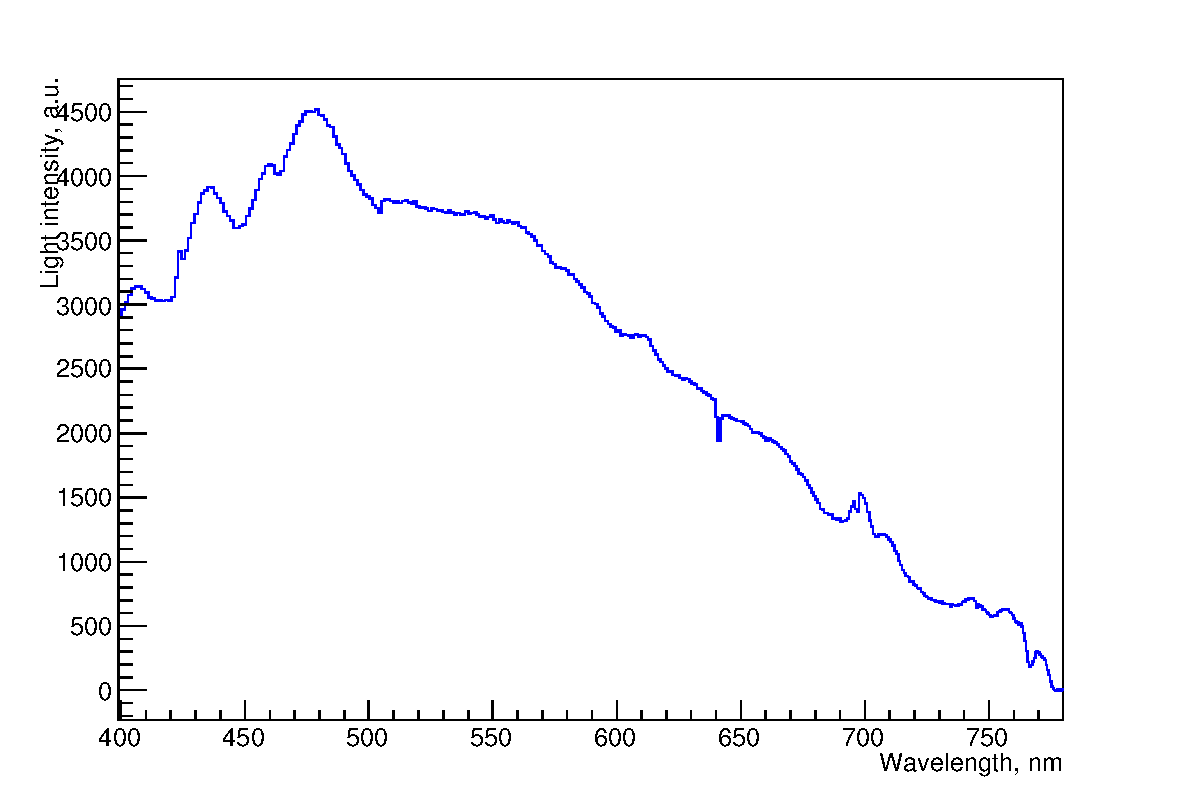
\includegraphics[width=\textwidth]{hv/spectro_spark}
	\caption[\glsentryshort{hv} test spark spectrum]{%
		Spectrum of the spark for a breakdown from a \SI{4}{\centi\metre} diameter cathode at \SI{-39.7}{\kilo\volt} and \SI{4.0}{\milli\metre} apart from the anode plate.
		The spectrum was integrated over a time of \SI{1}{\milli\second}.
	}
	\label{fig:hv_spectro_spark}
\end{figure}

Finally, when the streamer reaches the anode, a short peak of light emission is registered (frame \num{11} in Figure~\ref{fig:hv_images}) with the blue-green spectral component dominating (Figure~\ref{fig:hv_spectro_spark}).
This phase is characterised by an acoustic shock and a massive production of gas bubbles in the region of the discharge.
These effects are typical for an arc discharge in argon gas.
The spectrum of the light emission in this phase  is shown in Figure~\ref{fig:hv_spectro_spark}. 

As demonstrated in~\cite{Heindl} the transition from the liquid phase to the gas phase for scintillation manifests itself by the appearance of sharp spectral lines while in liquid the emission spectrum is continuous and without features.
This behaviour is also suggested by the two spectra in Figure~\ref{fig:hv_spectro}.
While the spectrum is continuous during the field emission phase, there is a distinct peak at around \SI{700}{\nano\metre} several \si{\milli\second} later.

It is worth mentioning that not every streamer results in a spark phase.
For those streamers started from the side of the cathode sphere the charge needed for streamer growth might exceed the total charge available in the system.
Such streamers extinguish before reaching the anode without an acoustic shock or any other additional effects.
On the other hand, in some cases the filament quickly transits to a third stage before it reaches the anode.
One possible explanation for this is that, if the filament current exceeds a given threshold, the filament loses its thermodynamic stability and expands into a gas bubble, in which the arc discharge quickly develops afterwards.

\begin{figure}[p]
	\centering
	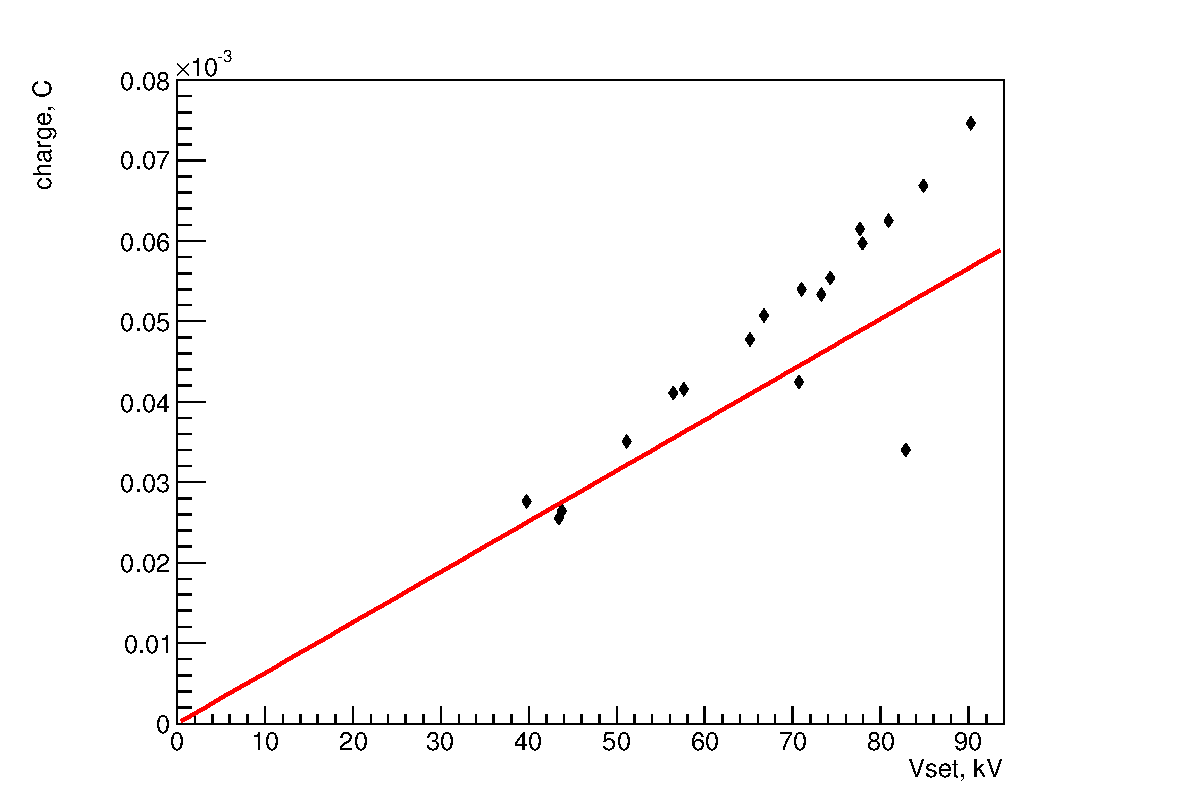
\includegraphics[height=0.43\textheight]{hv/selected_chargeVsVset}
	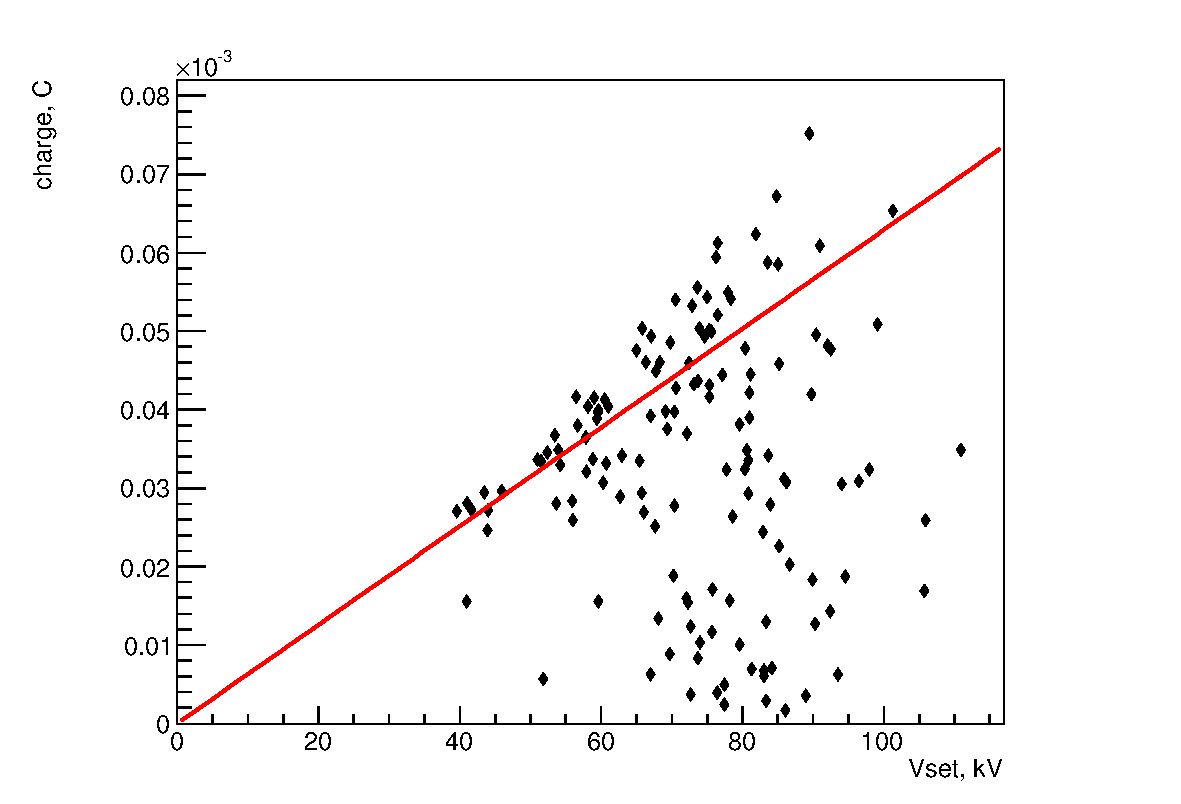
\includegraphics[height=0.43\textheight]{hv/allGood_chargeVsVset}
	\caption[\glsentryshort{hv} test integrated charge versus breakdown voltage]{%
		Correlations between integrated charge and breakdown voltage \emph{Vset} for the selected events with distinguishable slow streamer phase (top) and for all events with recorded current characteristics (bottom).
		The red line represents the charge stored in the gap capacitance using the tuned value of the latter.
	}
	\label{fig:hv_chargeVsVset}
\end{figure}

\begin{figure}[p]
	\centering
	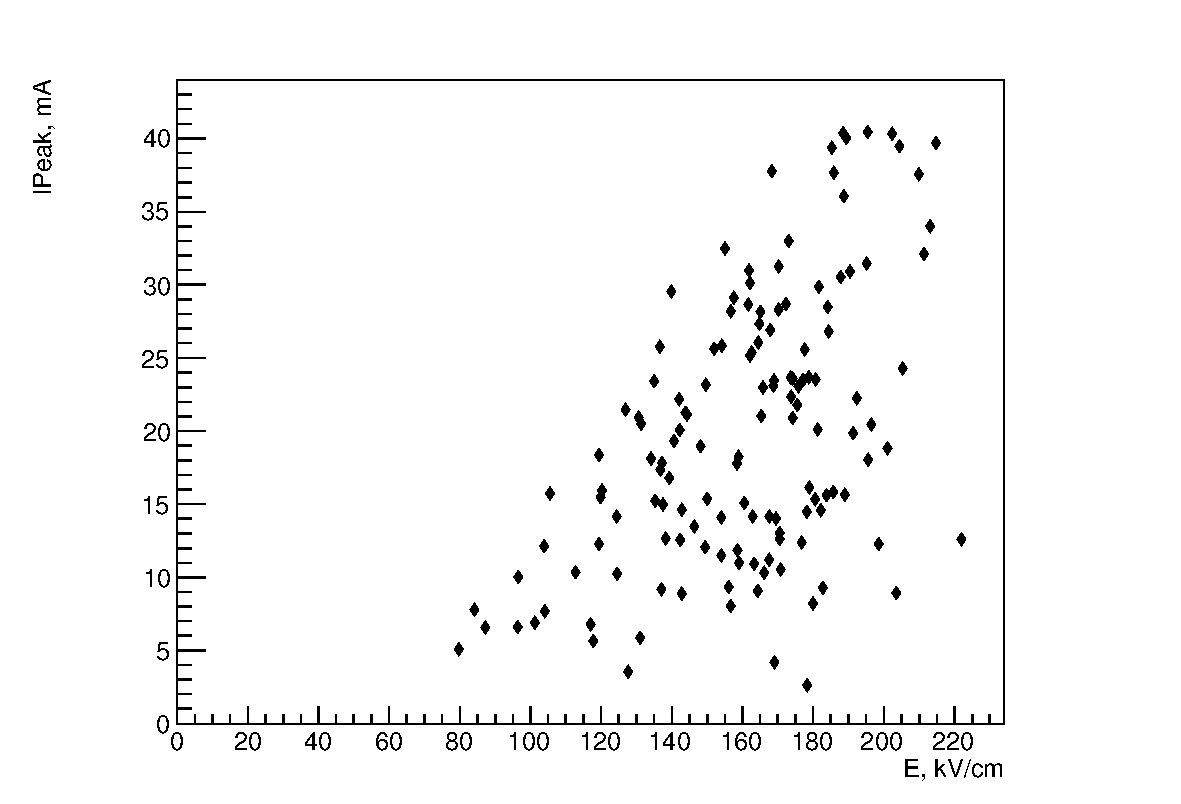
\includegraphics[height=0.4\textheight]{hv/allGood_IPeakVsE}
	\caption[\glsentryshort{hv} test peak current versus maximum breakdown field]{%
		Correlations between peak current \emph{IPeak} and maximum breakdown field \emph{E} for all events with recorded current characteristics.
	}
	\label{fig:hv_IPeakVsE}
\end{figure}

\begin{figure}[p]
	\centering
	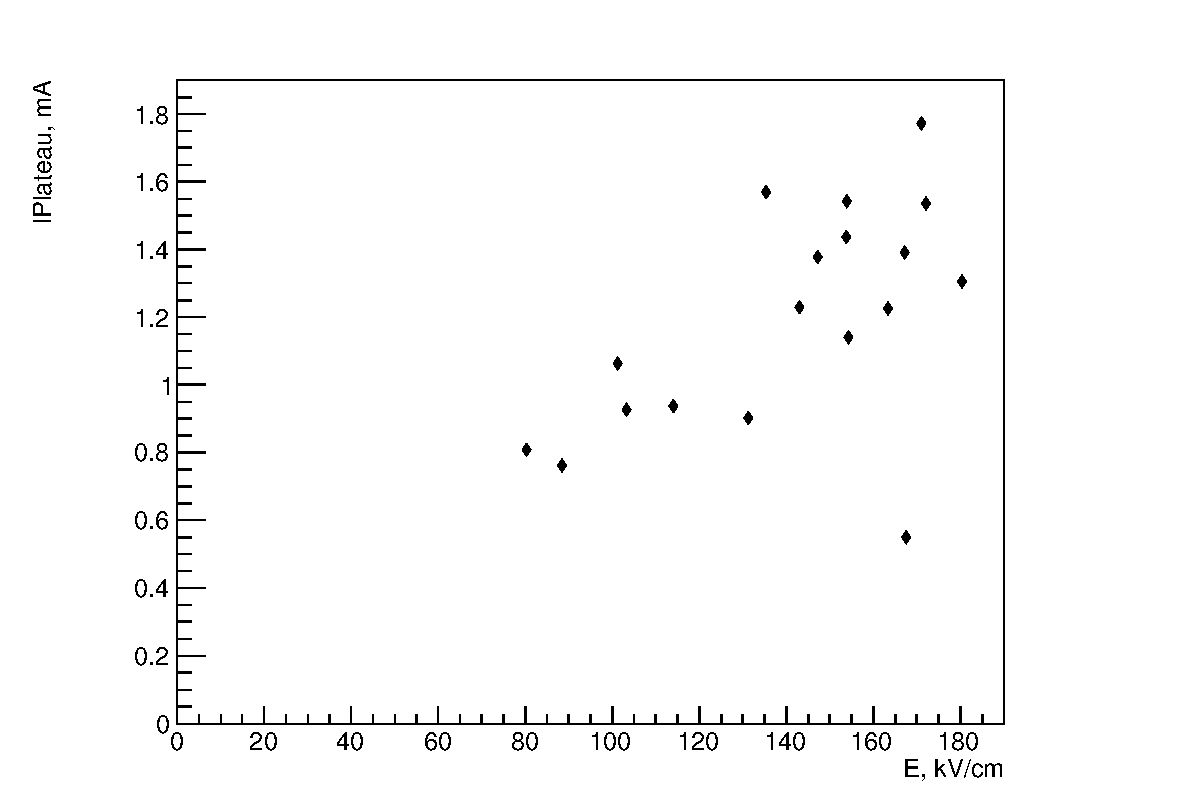
\includegraphics[height=.4\textheight]{hv/selected_IPlateauVsE}
	\caption[\glsentryshort{hv} test plateau current versus maximum breakdown field]{%
		Correlations between plateau current \emph{IPlateau} and maximum breakdown field \emph{E} for the selected events.
	}
	\label{fig:hv_IPlateauVsE}
\end{figure}

\begin{figure}[p]
	\centering
	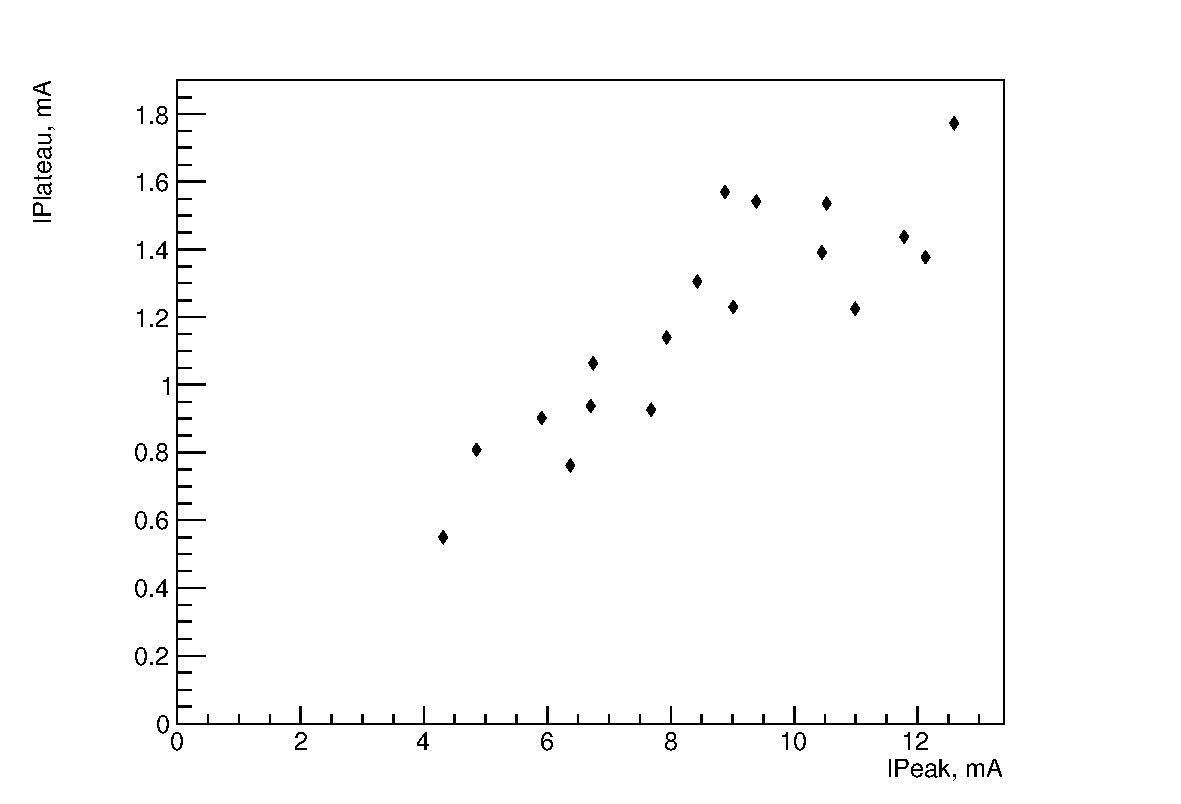
\includegraphics[height=.4\textheight]{hv/selected_IPlateauVsIPeak}
	\caption[\glsentryshort{hv} test plateau current versus peak current]{%
		Correlations between plateau current \emph{IPlateau} and peak current \emph{IPeak} for the selected events.
		}
	\label{fig:hv_IPlateauVsIPeak}
\end{figure}

\begin{figure}[p]
	\centering
	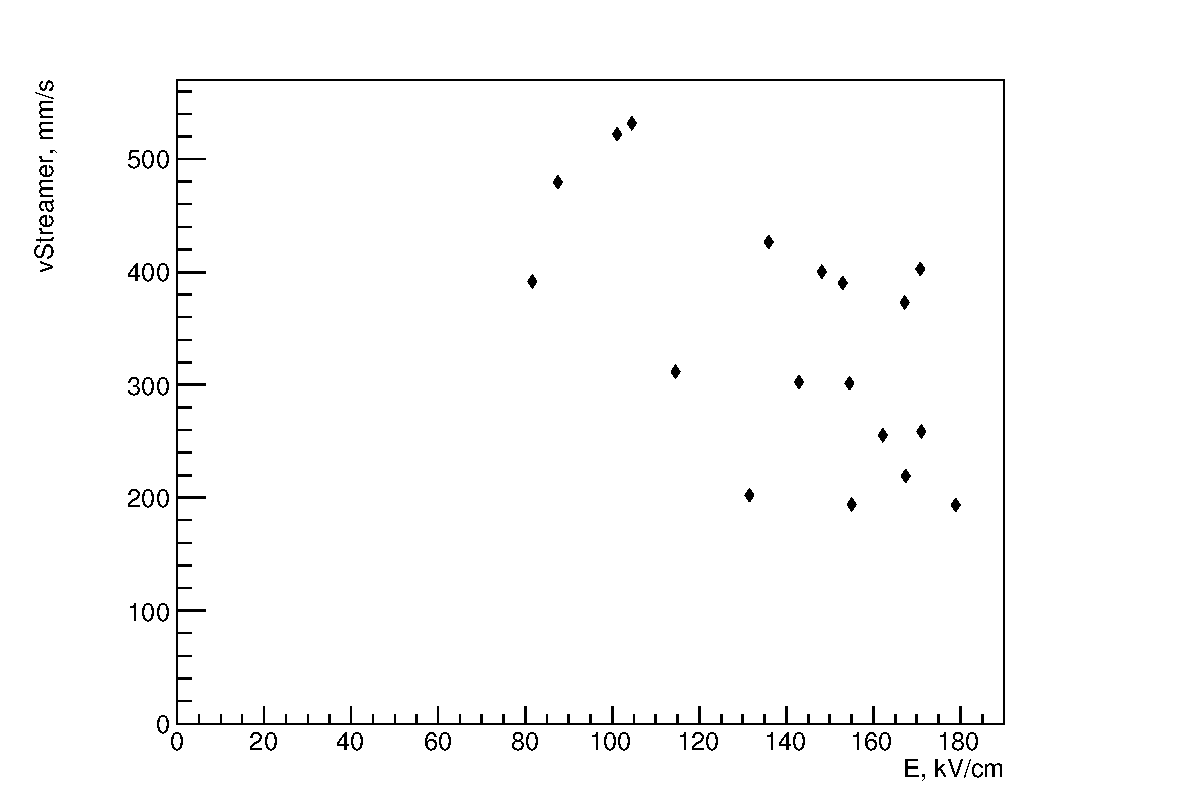
\includegraphics[height=.4\textheight]{hv/selected_vStreamerVsE}
	\caption[\glsentryshort{hv} test minimum streamer velocity versus maximum breakdown field]{%
		Correlations between minimum streamer velocity \emph{vStreamer} and maximum breakdown field \emph{E} for the selected events with a distinguishable slow streamer phase.
	}
	\label{fig:hv_vStreamerVsE}
\end{figure}

In Figures~\ref{fig:hv_chargeVsVset} to~\ref{fig:hv_vStreamerVsE} several correlations of measured and calculated parameters of the breakdowns are shown.
For some of these plots \num{18} events were selected with recorded current characteristics similar to Figure~\ref{fig:hv_iv}.
As a comparison the bottom plot of Figure~\ref{fig:hv_chargeVsVset} shows the data of all events with current characteristics including events not possessing a distinct plateau as the one visible in Figure~\ref{fig:hv_iv}.
The discrepancy to the total number of events in Table~\ref{tab:hv_table2} arises, on the one hand, because the shunt resistor was installed only in the last run and, on the other hand, since the resistor was damaged after the events shown in the bottom plot of Figure~\ref{fig:hv_chargeVsVset}.
The low number of events in the selection is due to the fact that an automated analysis of the current characteristics can only detect very long streamers.
This also explains the behaviour of the charge in Figure~\ref{fig:hv_chargeVsVset}.
The selected streamers last for several \si{\milli\second}, almost always consume the whole charge in the system, and then cease without transitioning to a spark.
The slight excess in charge compared to the charge in the gap capacitance (red line) is likely supplied by the \gls{psu} before tripping.
Contrary to this the bottom plot showing all the events contains many events that do not consume all the stored charge and result in a spark.
The good match between the red curve and the data points serves as a cross-check of the tuned capacitance.

Figure~\ref{fig:hv_IPeakVsE} shows the behavior of the peak current versus the breakdown field, suggesting a proportionality between the two with a coefficient of about \SI{60}{\micro\ampere\centi\metre\per\kilo\volt}.
The field was calculated by dividing the breakdown voltage by the gap distance.
Therefore, this is a mean value along the shortest path and only an upper limit for most of the selected events because the streamer often emerged from the side of the sphere.

Figures~\ref{fig:hv_IPlateauVsE} and~\ref{fig:hv_IPlateauVsIPeak} show the correlation of the current during the streamer phase (the plateau in Figure~\ref{fig:hv_iv}) with the breakdown field and peak current, respectively.
The plateau current clearly rises with both, breakdown field and peak current.
Together with Figure~\ref{fig:hv_IPeakVsE} this indicates that for higher fields higher currents flow during the field emission phase as well as the streamer phase.
As mentioned above the plateau current could only be reliably detected for the selected events, which is why these plots are not shown for all events.

Finally, Figure~\ref{fig:hv_vStreamerVsE} depicts the dependence of the streamer velocity on the breakdown field.
Again, the velocity is only a lower limit as it was calculated by dividing the gap distance by the duration of the streamer, which is not correct for streamers emerging from the side of the sphere.
There are two distinct types of events.
While the selected streamers are rather slow (velocity $\approx \SI{300}{\milli\metre\per\second}$, independent of the field), the whole data set contains much faster events with the total time in the \si{\nano\second} scale (not shown).
The knowledge of the streamer velocity can be applied in the design of protection circuits for future \lartpc{}s.
If a breakdown condition is detected during the streamer phase, the \gls{hv} can be killed prior to a disruptive spark phase potentially damaging sensitive detector electronics.


\section{A Method to Suppress Electric Breakdowns in \glsentrylong{lar}}
\label{sec:studies_latex}

As a result of the thorough characterisation of breakdowns in \lar{} a way was found to suppress them by coating \gls{hv} components with latex.
It was possible to increase the voltage by a factor of \num{10} using this technique.
This study has been published in~\cite{latex}.

The setup was the same as the one used to study the breakdowns, described in Section~\ref{sec:studies_breakdown}.
Additionally, the cathode sphere was coated by a layer of polymer.
In order to effectively suppress electric breakdowns the coating needs to have a high dielectric strength while at the same time staying elastic at cryogenic temperatures (\SI{87}{\kelvin} for a \lar{} detector).
Furthermore, the excess electron mobility of the coating needs to be significantly lower than the one of \lar{}.
If this is the case, electrons emitted by the cathode via field emission can accumulate inside the coating layer and in turn locally reduce high fields and thus quench the field emission.

Natural polyisoprene (latex rubber) is a polymer that satisfies the above requirements.
Its dielectric strength is reported to be in the range of \SIrange{1}{2}{\mega\volt\per\centi\metre}~\cite{fizikaDielektrikov}, its dielectric constant is \num{2.1} which is close to the \num{1.6} of \lar{}, and its room temperature resistivity is \SI{1e16}{\ohm\centi\metre}.
A polyisoprene layer of several \SI{100}{\micro\metre} can be deposited on the sphere by dipping the latter in purified latex milk.
After drying at room temperature the coating is leached in deionised water for several hours and finally vulcanised at \SI{70}{\celsius} for one hour.
Leaching is needed to remove all soluble pollutants contained in natural latex while the vulcanisation increases the tear strength of the coating.
Like this the polyisoprene layer keeps its integrity and does not crack even after multiple fast cool-down and warm-up cycles to \SI{87}{\kelvin} and back to room temperature, respectively.

In the first measurement a \SI{4}{\centi\metre} cathode sphere coated with \SI{450}{\micro\metre} of polyisoprene was used.
The test was started at a cathode anode gap width of \SI{5}{\milli\metre} and the voltage was ramped up from \SIrange{0}{130}{\kilo\volt} at \SI{50}{\volt\per\second}.
After no breakdown could be observed for several hours, the gap width was decreased to \SI{4}{\milli\metre}.
The voltage was ramped down for the gap adjustment and ramped back up afterwards.
Again, no breakdown occurred for several hours and subsequently the gap was decreased to \SI{3}{\milli\metre}.
During the third ramp-up there was a breakdown at \SI{112}{\kilo\volt}.
This corresponds to a maximum electric field intensity across the gap of \SI{412}{\kilo\volt\per\centi\metre}, which is more than one order of magnitude higher than the required value to provoke breakdowns from an uncoated cathode~\cite{breakdown_14, breakdown_16}.
A summary of the results is given in Table~\ref{tab:latex_table1}.

\begin{table}[htb]
	\centering
	\caption[\glsentryshort{hv} coating test summary]{%
		Summary of the breakdown test measurements with \SI{200}{\micro\metre} and \SI{450}{\micro\metre} thick polyisoprene layers deposited on \SI{5}{\centi\metre} and \SI{4}{\centi\metre} diameter spherical cathodes, respectively.
	}
	\label{tab:latex_table1}
	\begin{tabu} to \textwidth {SSSSl}
		\toprule
		{$d_{\m{Gap}} \qty[\si{\milli\metre}]$} &	{$E_{\m{max}} \qty[\si{\kilo\volt\per\centi\metre}]$} &	{$\varnothing_{\m{Sphere}} \qty[\si{\centi\metre}]$} &	{Polyisoprene thickness $\qty[\si{\micro\metre}]$} &	Breakdown \\
		\midrule
		5.0 &	298 &	4 &	450 &	no \\
		4.0 &	358 &	4 &	450 &	no \\
		3.0 &	412 &	4 &	450 &	yes \\
		3.0 &	296 &	5 &	200 &	yes \\
		\bottomrule
	\end{tabu}
\end{table}


\section{\glsentrylong{hv} Summary}
\label{sec:studies_hv-summary}

A study of the visible light emission by electrical breakdowns in \lar{} was performed, near its boiling point with cathode-anode distances ranging from \SIrange{0.1}{10.0}{\milli\metre} with a spherical cathode and a plane anode geometry.
Three distinct discharge development phases were identified by observing the discharge appearance and the time development of the visible light emission.
The dependence of several breakdown parameters on the critical field was also studied.
For the first time it was found that the streamer propagation velocity is about \SI{300}{\milli\metre\per\second} and independent of the field intensity.
The streamer phase is characterised by a current peak between \SIlist{5; 15}{\milli\ampere} depending on the breakdown field, followed by a plateau at an approximately ten times lower current level.

The deposition of a few hundred \si{\micro\metre} thick polyisoprene (latex) layer on the surface of a spherical stainless steel cathode immersed in \lar{} serves to efficiently suppress field emission of electrons from the cathode surface.
As a result significantly higher electric field intensities can be reached for cathode-ground distances of several \si{\milli\metre}.
A field strength as high as \SI{412}{\kilo\volt\per\centi\metre} was reached.
This solution enables the operation of \lartpc{}s with a \lar{} volume outside the electron drift region much smaller compared to \lartpc{}s with non-coated cathode surfaces.

However, it was also found that the employed latex coating is very fragile.
In particular, it loses its protective function after a single breakdown.
This makes an application in a physics experiment impractical.
Currently, a safe \lartpc{} operation can only be guaranteed by keeping electric fields below \SI{40}{\kilo\volt\per\centi\metre} at all points in the detector.
Therefore, either low cathode voltages or large inactive volumes around the cathode are required.
	\section{Charge Readout}
\label{sec:studies_charge-ro}

As outlined in Section~\ref{sec:lartpc_challenges}, classical wire readouts pose two big challenges to future \lartpc{}s: ambiguities and mechanical stability.
Two new charge readout concepts were tested for this work.
Wires implemented as printed circuits solve the mechanical problems but not the ambiguities.
A pixelated charge readout solves both problems but introduces a new one of a drastically increased number of reaodut channels.


\subsection{A More Robust Approach to \glsentryshort{tpc} Readout Wires}
\label{sec:studies_charge-ro_cuoka}

A possible solution to the mechanical problems with wires is to not use actual wires but instead print thin coper tracks on a support structure.
To investigate this solution, a proof of concept was performed at \gls{help}.

In a classical wire readout plane, the induction signal is produce by drifting the charge through one or multiple induction wire grids.
With the proposed scheme of copper tracks on a support structure, it is no longer possible for the charge to actually drift through the induction plane(s).
Therefore, induction is only produced by the approach of the charge.
One consequence of this is, that induction signals will no longer bi bipolar.
As opposed to the classic design, the collection plane will even be in front of the induction plane(s).
This means that the charge can only approach the induction plane(s) until it is collected by the collection plane on the top layer of the support structure.
That is why it is crucial to make the support structure as thin as possible in order to get induction signals as high as possible.
Using a \gls{fr4} structure as in classical \gls{pcb} designs is therefore not a viable option.
Very thin support structures can be provided by using a flexible \gls{pcb} made from Kapton instead of \gls{fr4}.
These can be made as thin as a few \SI{10}{\micro\metre}.
For this test, a Kapton layer of \SI{50}{\micro\metre} was used with a single induction plane on the back (Fig.~\ref{fig:cuoka_readout-plane}).
The Kapton layer was supported by an \gls{fr4} frame for mounting on the \gls{tpc}.

\begin{figure}[htb]
	\centering
	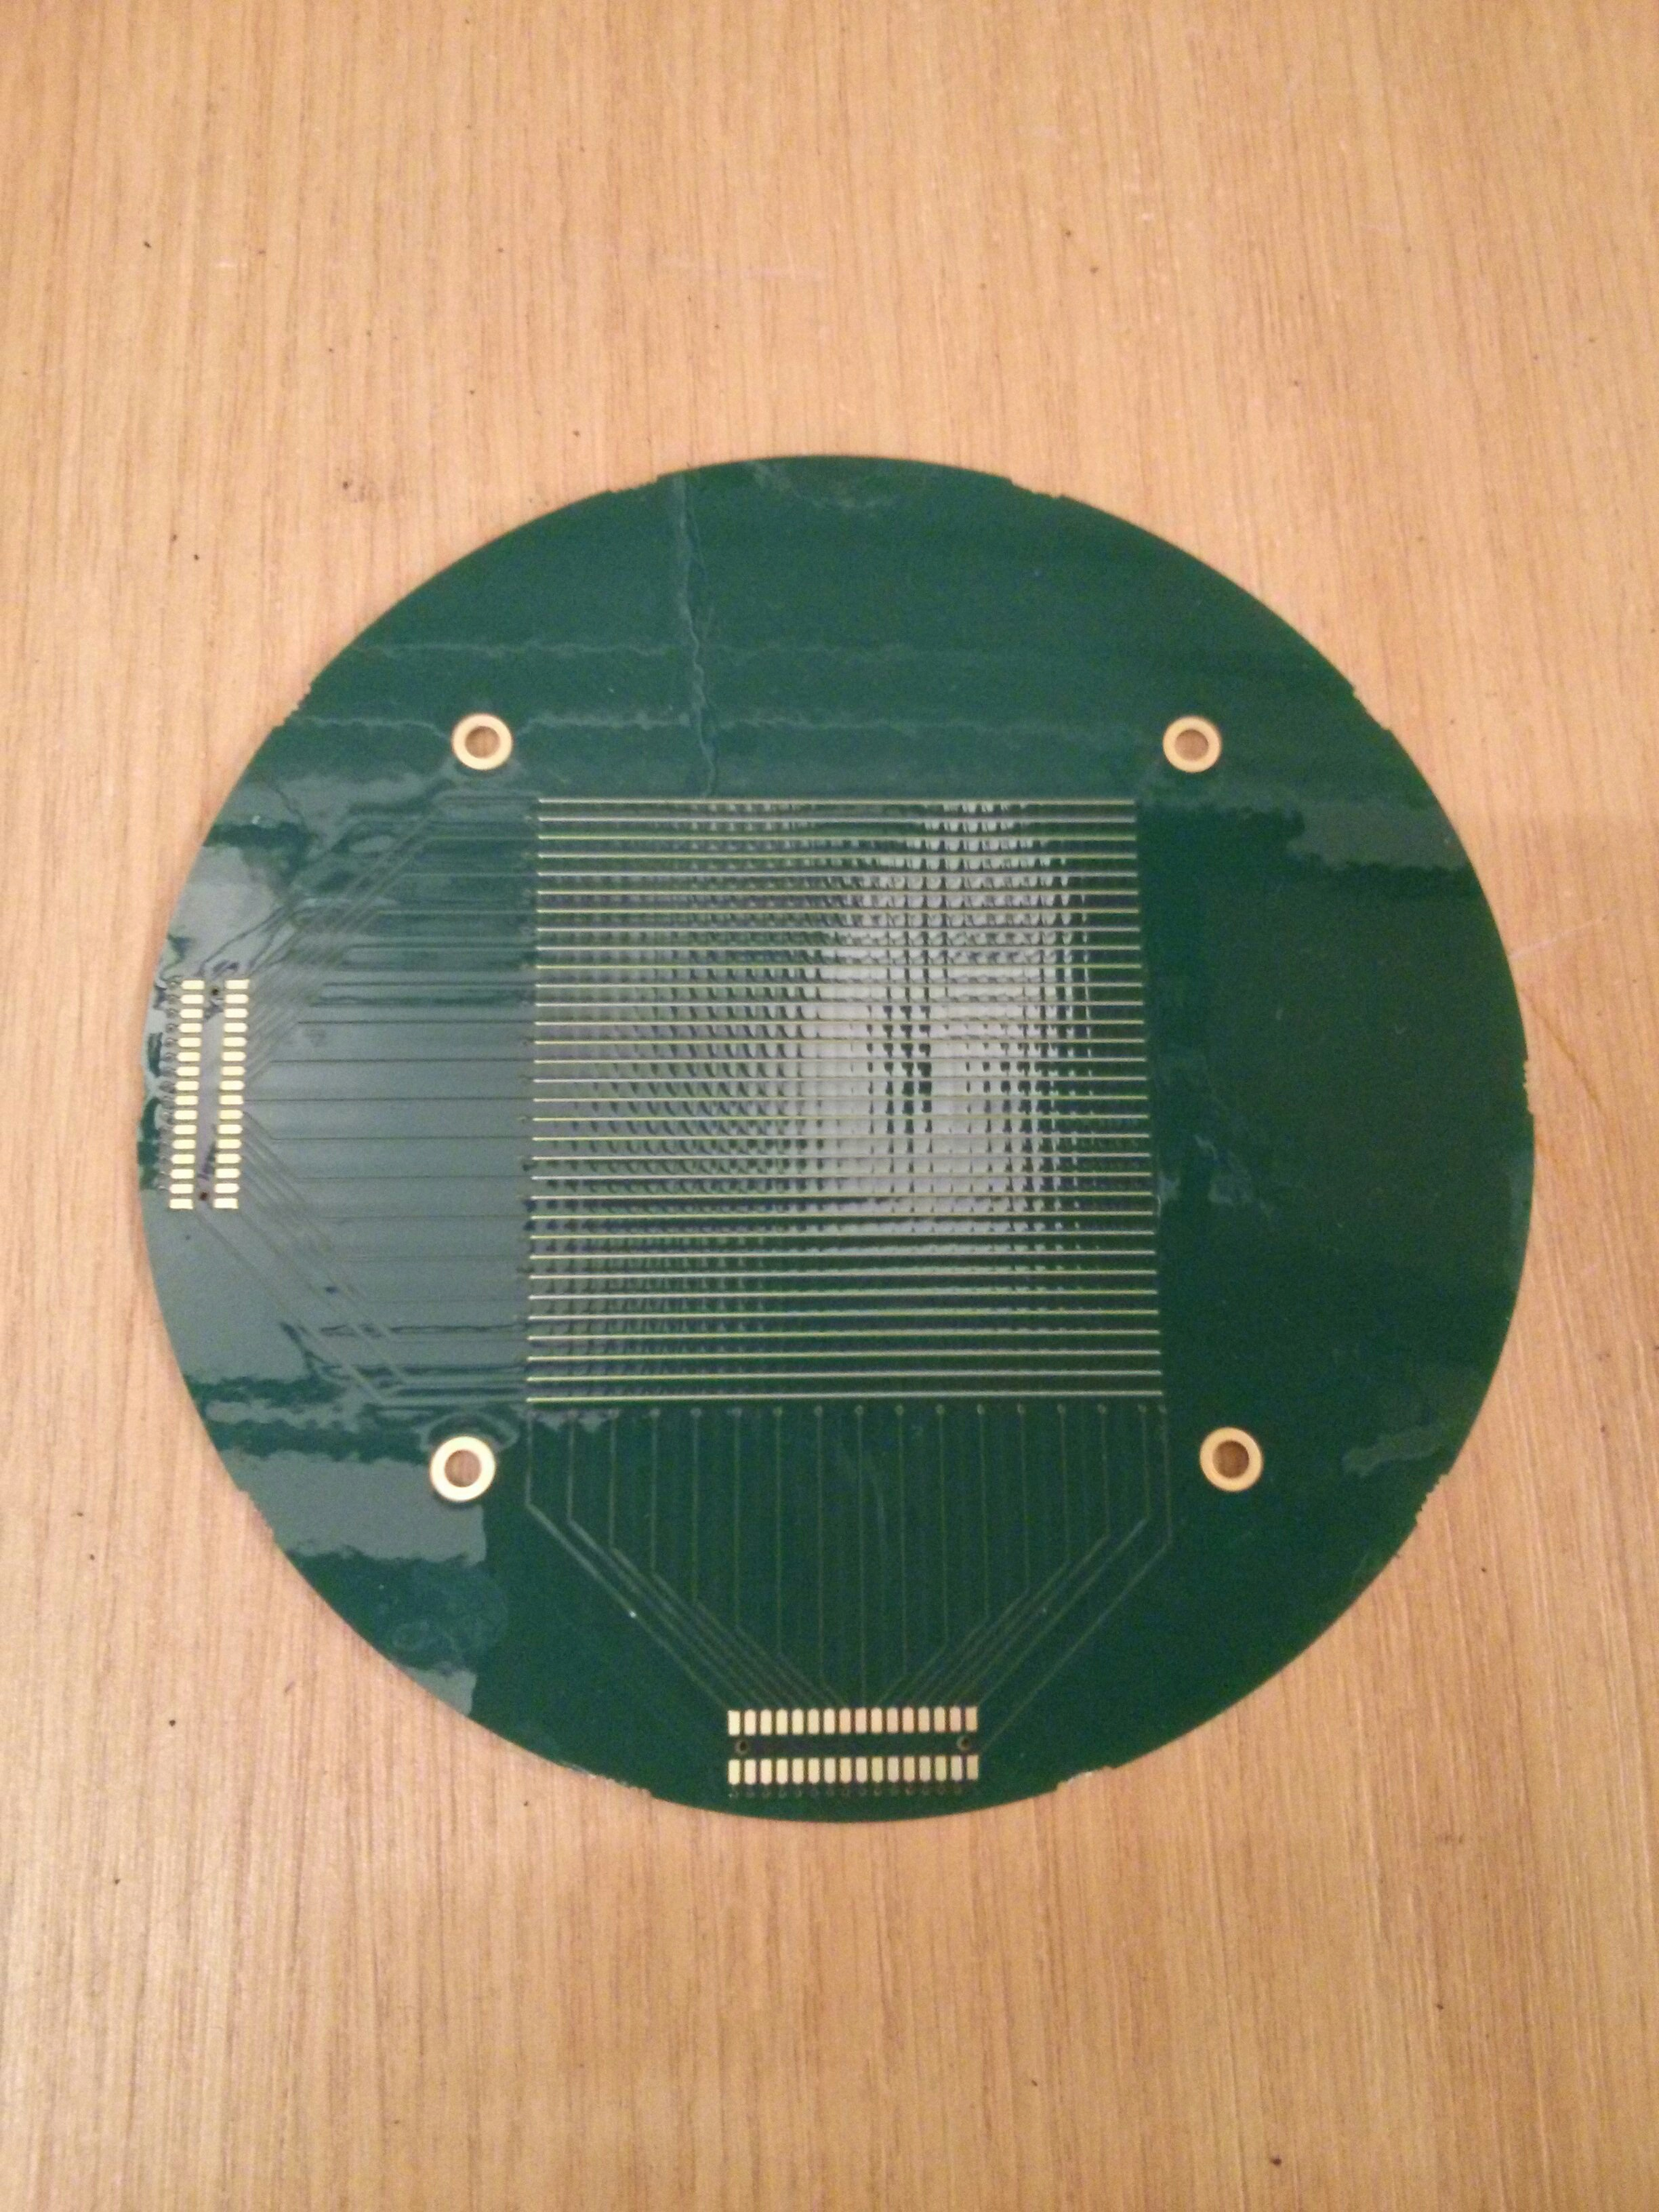
\includegraphics[width=0.5\textwidth]{cuoka/readout_plane_bottom}
	\caption{Copper on Kapton readout plane.}
	\label{fig:cuoka_readout-plane}
\end{figure}

The test was performed in a small vacuum-insulated double-batch cryostat with an inner volume of \SI{30}{\centi\metre} diameter and \SI{50}{\centi\metre} height.\todo{check dimensions}
Prior to filling, the cryostat was evacuated using a turbo-molecular pump and then purged with argon gas and evacuated a second time.
From earlier experiments~\cite{2photonAbs}, the purity can be assumed to be $\sim{\SI{1}{ppb}}$ after filling.
The cryostat is sealed using rubber o-rings which lose tightness at cryogenic temperatures.
Therefore, and due to the fact that no purification system was available, the purity degraded slowly in the course of the experiment.
The \SI{8}{\centi\metre} long field cage consists of \num{8} copper rings of \SI{8}{\centi\metre} diameter terminated by a copper plate cathode.
A field of \SI{1}{\kilo\volt\per\centi\metre} is generated using a resistive divider.

\begin{figure}[htb]
	\centering
	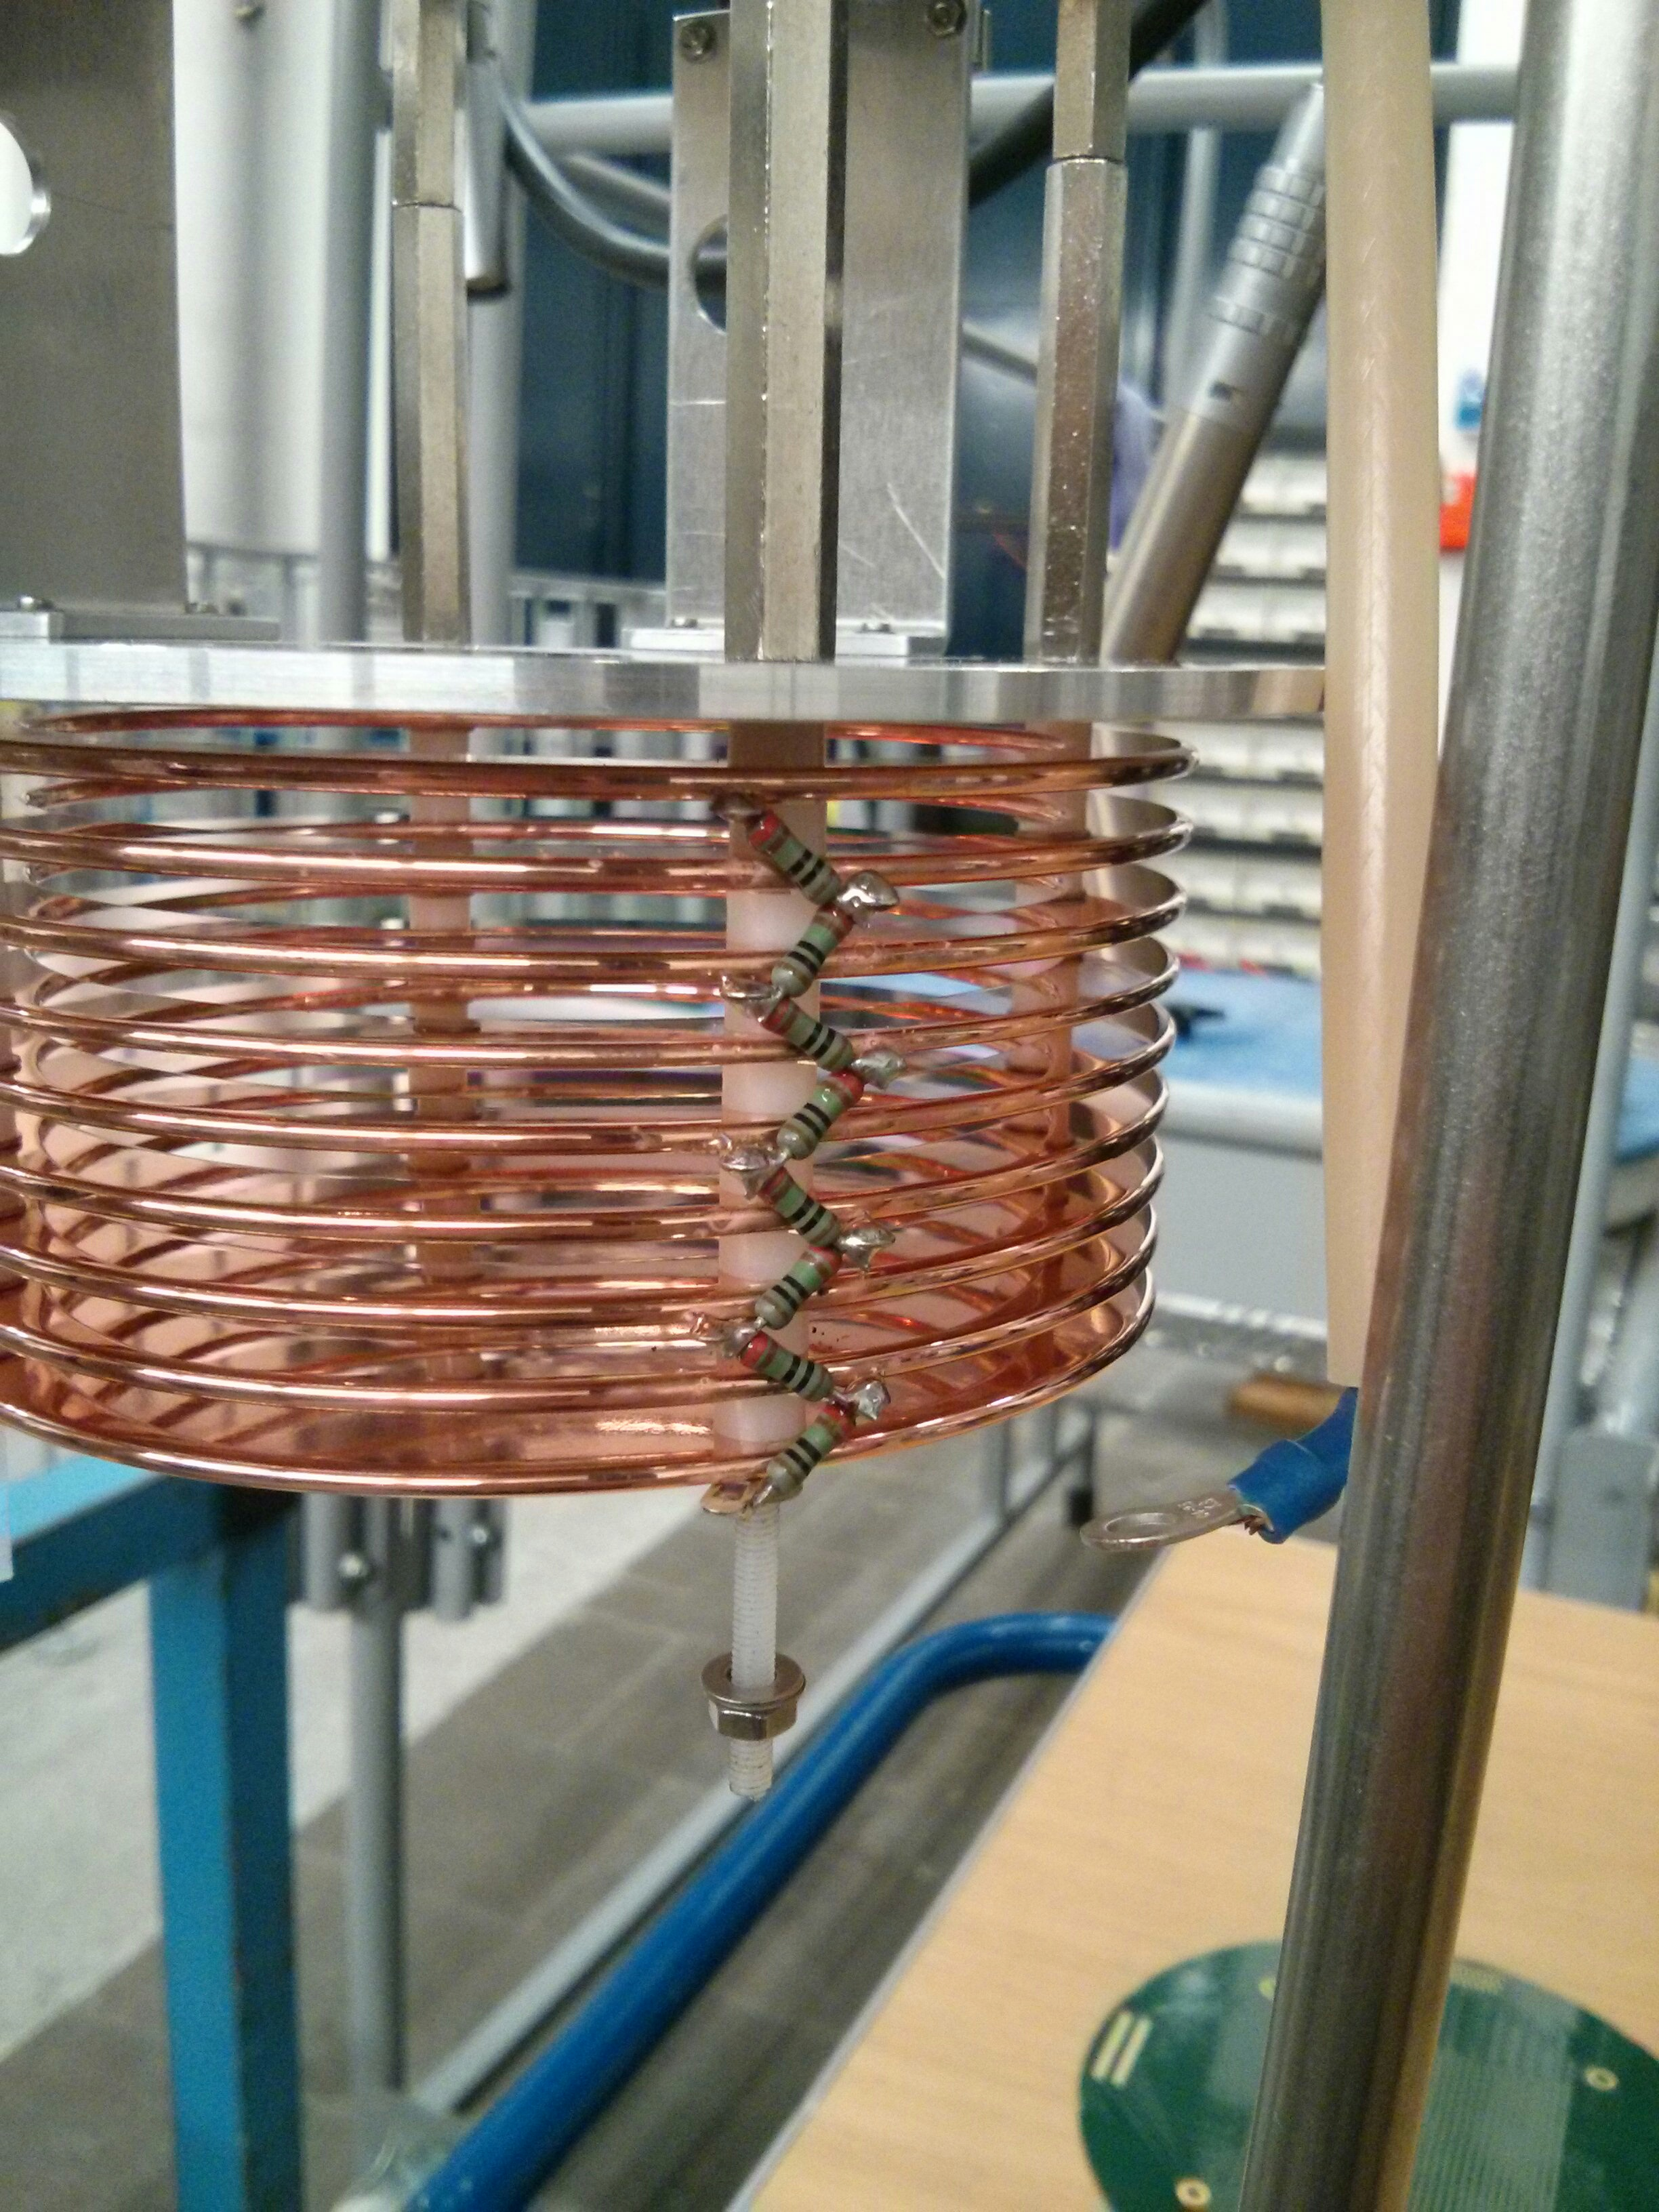
\includegraphics[width=0.5\textwidth]{cuoka/tpc}
	\caption{\gls{tpc} used for the copper on Kapton readout test.}
	\label{fig:cuoka_tpc}
\end{figure}

The charge readout electronics were adopted from \AT{} without modifications.
Charge signals are amplified by cryogenic charge amplifiers and then digitised at room temperature.
More details can be found in Section~\ref{sec:studies_electronics_at}.

Because of the limited space inside the cryostat, no internal light triggering system could be used.
Instead, the digitisers were either triggered on one of the charge collection channels or by an external muon telescope.
The latter was formed of two scintillator panels with \glspl{pmt}s above and below the cryostat, respectively.
Triggering directly on charge collection channels has the potential disadvantage of recording events only partially.
If the triggering channel does not receive the first charge pulse of the event, all earlier pulses are lost, unless the \gls{daq} implements a pretrigger ring buffer of sufficient size.
It is therefore preferable to trigger on the external muon telescope.

Using the above-described setup, cosmic muons were recorded over the course of multiple hours.
A typical event is depicted in Figure~\ref{fig:cuoka_event}.
It can be seen that due to the event being almost parallel to the induction strips, the induction signal is in fact stronger than the collection signal.
The reason for the bad \gls{snr} is improper grounding of the setup and high noise levels in the lab from the nearby train station and air conditioning.
Due to time constraints and an upcoming test of a pixelated readout described in Chapter~\ref{chap:dune-nd}, no analysis was performed on this data.
Anyhow, the fact that cosmic muons could be seen using this setup proves that there is no inherent problem with having the induction plane a few \SI{10}{\micro\metre} behind the collection plane.

\begin{figure}[htb]
	\centering
	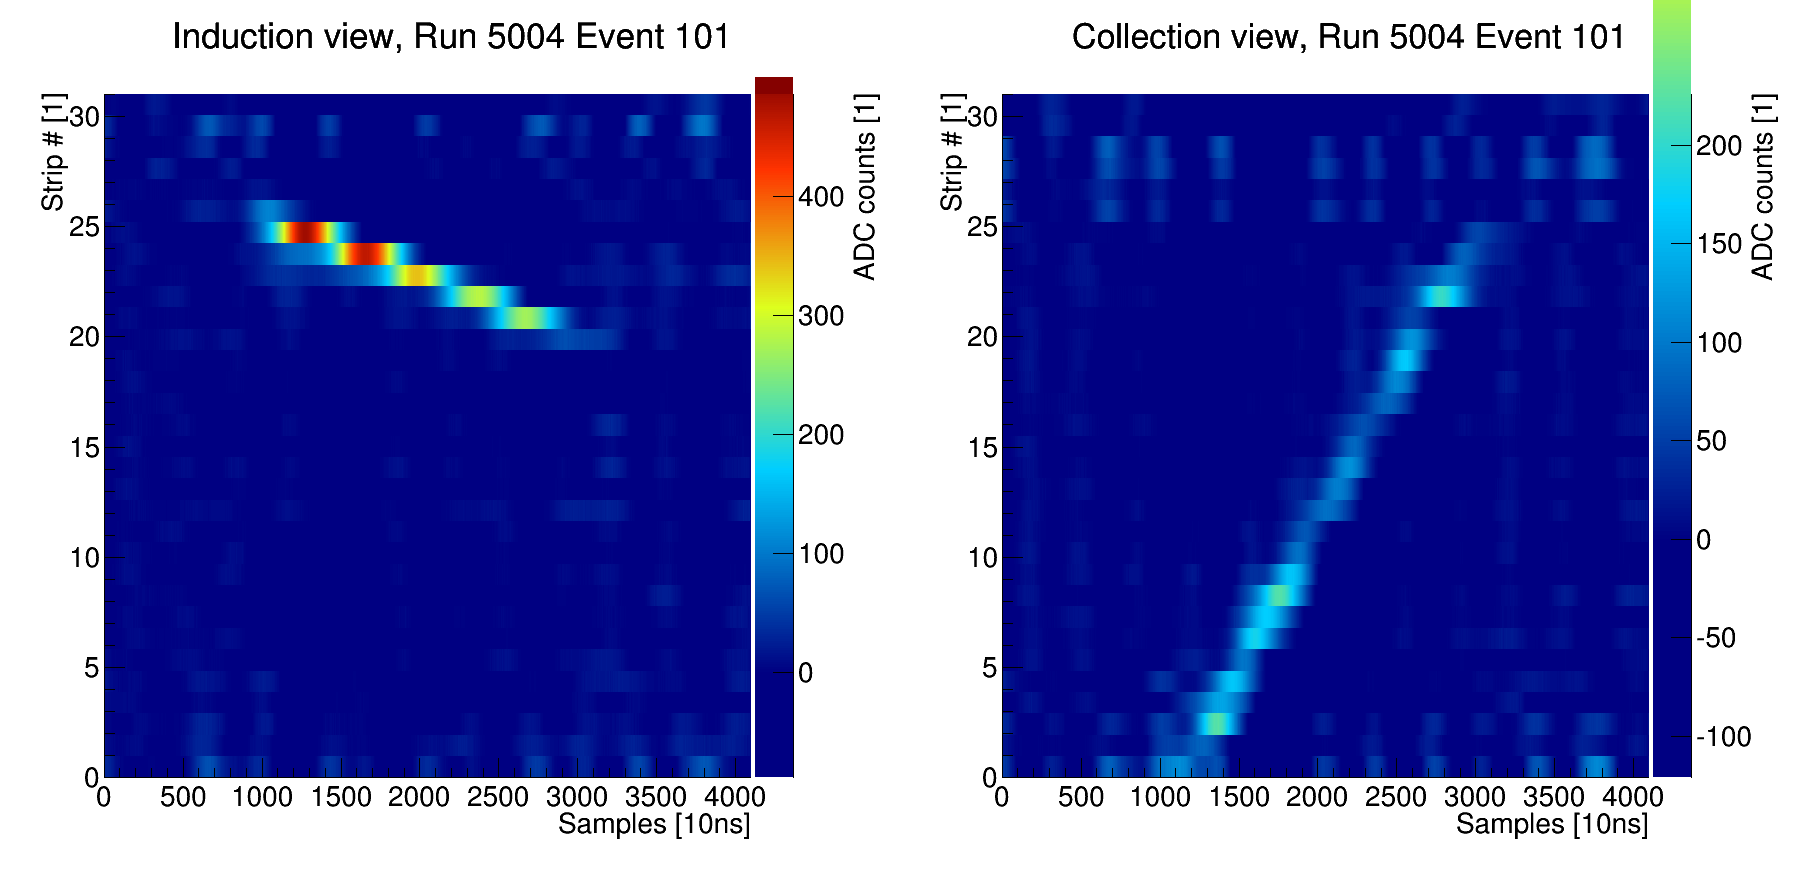
\includegraphics[width=\textwidth]{cuoka/muon_event}
	\caption{Muon event recorded using the copper on Kapton readout.}
	\label{fig:cuoka_event}
\end{figure}

While this technique can potentially solve the mechanical problems of classical wire readouts, it does not reduce the ambiguities inherent to 2D-projective readouts outlined in Section~\ref{sec:lartpc_challenges}.
Because of this, it was decided not to further investigate copper on Kapton readouts and instead focus on pixelated readouts for \lartpc{}s providing real 3D data.


\subsection{Pixel Readout}
\label{sec:studies_charge-ro_pixel}

As outlined in Section~\ref{sec:lartpc_challenges}, wire readouts are not suitable for \lartpc{}s the size of the envisioned future neutrino detectors.
The ambiguities caused by the nature of wire readouts can be eliminated by using a fully pixelated readout.
Such a readout will record a true 2D image of the charge for every time slice and thus directly produce 3D space points of the event.
On the other hand, this will increase the required number of \gls{daq} channels and therefore the data throughput.
To illustrate this, let us imagine a readout plane of \SI{1 x 1}{\metre} and a desired resolution of \SI{5}{\milli\metre}.
For a conventional wire readout with two planes, this results in

\begin{IEEEeqnarray}{rCl}
	\qty(\frac{\SI{1}{\metre}}{\SI{5}{\milli\metre}}) \times 2 & = & 40
\end{IEEEeqnarray}

wires and thus \gls{daq} channels.
In order to reduce ambiguities, one can use more than two planes which will increase the number of channels linearly with the number of planes.
For a pixelated readout,

\begin{IEEEeqnarray}{rCl}
	\qty(\frac{\SI{1}{\metre}}{\SI{5}{\milli\metre}}) ^ 2 & = & 400
\end{IEEEeqnarray}

\gls{daq} channels are required.
Scaling this up to the needed detector size, this leads to an enormous number of \gls{daq} channels and data throughput.

It is possible to reduce the number of channel by employing some form of multiplexing.
There are multiple options, one could imagine for this:
\begin{itemize}
	\item Digital multiplexing
	\item Genetic multiplexing
	\item \glspl{roi}
\end{itemize}

Digital multiplexing means digitising all channels as close as possible to the readout plane and then mutliplexing the digital data onto a high-speed digital link.
An advantage of this technique is that the technology for this already exists and is well established in information technology.
Ideally, one would feed the data stream into an optical fibre which additionally would provide galvanic isolation of the readout from the \gls{daq}.
The challenging part is that all of this needs to happen at cryogenic temperatures which is far from trivial because most off-the-shelf components are not made for this.
A detailed description of upcoming electronics capable of cold digitisation an multiplexing is given in Section~\ref{sec:studies_electronics_pixel}.
In contrast, genetic multiplexing and \glspl{roi} are forms of analogue multiplexing.
The difference to digital multiplexing is that multiple readout channels are combined into a single analogue link before digitising them at room temperature outside the cryostat.
In the two schemes described here, this happens by connecting multiple readout channels to a single \gls{daq} channel.

In genetic multiplexing, the connections are done in a way that a certain event type (a single straight track for instance) forms a distinct pattern of \gls{daq} channels activated.
For simple events, it is possible to recover the full event from the pattern.
Naturally, this reintroduces new ambiguities.
Depending on the complexity of the event topology and the degree of multiplexing, they can potentially be resolved during reconstruction.
In any case, if the event is too complex, it cannot be reconstructed properly.
While genetic multiplexing has been shown to work for one-dimensional readouts (wires), there is no known solution for two dimensions (pixels).\todo{sauce}

A third technique is to subdivide a pixelated readout plane in so-called \glspl{roi}.
This scheme was tested for an earlier PhD thesis at \gls{help} using a \gls{micromegas} in a xenon gas \gls{tpc}~\cite{maplesyrup}.
All pixels at the same position inside the \glspl{roi} are connected to the same \gls{daq} channel.
For instance, let us assume squared \glspl{roi}.
One \gls{daq} channel would connect to all the pixels in the top left corners of the \glspl{roi}.
Another channel would connect to all the pixels in the top right corner and so on.
To explain this a little better, let us assume a square pixel plane of $N \times N$ pixels where $N = n ^ 2$ with an arbitrary integer $n$.
Now, we divide the plane into $n \times n = N$, each consisting again of $n \times n = N$ pixels.
For such a readout, we require $N$ \gls{daq} channels for the \glspl{roi} and another $N$ channels for the pixels.
We need only as many pixel channels as we have pixels per \gls{roi} because all the pixels at the same relative position inside the \glspl{roi} are connected together to one \gls{daq} channel.
This means that we can read out a $N \times N$ pixel plane using only $2 N$ \gls{daq} channels; the same number required by a conventional 2-plane wire readout of the same size and pitch.
If there is a signal on a certain \gls{daq} channel, the position inside the \gls{roi} is known but not the \gls{roi}.
To determine the full position, each \gls{roi} has its own inductive grid in between the pixels.
The grid is biased such that the charge is fully focussed onto the pixels and does not collect any charge.
Combining the bipolar pulse on the \gls{roi} grid with the collection pulse from the pixels, it is possible to disentangle the true position.
Again, the drawback of this approach is that it is not free of ambiguities.
It fails for multiple simultaneous hits when it is impossible to say which pixel pulse belongs to which \gls{roi} pulse.

Independently of the amount of data one needs to bring out of the detector, a second problem is heat dissipation.
The more of the readout chain is sitting inside of the detector, the more serious this problem becomes.
It is especially problematic for digital multiplexing which requires a lot of cryogenic electronics.
A possible solution to this is to power only that part of the readout that is actually needed.
This would require a means to wake up the part of the readout where the charge is arriving before it is collected.
Provided, the wake-up time is short enough, inductive grids on \glspl{roi} could allow precisely for this.

As the \gls{roi} approach had already been demonstrated in a gas \gls{tpc}, it was chosen for the first prototype of a pixelated \lartpc{}.
Because the detector is a single-phase \lartpc{}, and thus no gas amplification as in \gls{micromegas} is needed, the readout plane could be realised as a conventional Printed Circuit Board \gls{pcb}.
Alongside the \gls{pcb}, a new \gls{tpc} was designed which can be reused for future prototyping efforts.
The design of \gls{pcb} and \gls{tpc} as well as the results from the first tests are described in Section~\ref{sec:ac_viper}.
	\section{Charge Readout Electronics}
\label{sec:studies_electronics}

For a heavy MIP with $\dv{E}{x} \approx \SI{2.1}{\mega\electronvolt\per\centi\metre}$, a \lartpc{} has a charge yield of $\sim{\SI{1}{\femto\coulomb\per\milli\metre}}$ as explained in Chapter~\ref{chap:lartpc}.
The readout electronics need to be able to reliably digitise this charge.
This chapter aims to outline the challenges based on present designs and then present several tests of future approaches addressing them.

One of the biggest challenges to detect such low charges is the \gls{snr}.
Noise can originate from a plethora of sources.
They can be divided into internal, originating inside the electronic components, and pick-up from external sources.

The most important internal source is the \emph{Johnson-Nyquist} noise.
It is generated by the intrinsic motion of the charge carriers at non-zero temperature therefore often called thermal noise.
In statistical thermodynamics, the energy of a system with one degree of freedom,
\begin{IEEEeqnarray}{rCl}
	E & = & \frac{k T}{2} \qc
\end{IEEEeqnarray}
is proportional to its temperature $T$ by the Boltzmann constant $k$.
The stored energy in a capacitor is given by
\begin{IEEEeqnarray}{rCl}
	E & = & \frac{C V ^ 2}{2} \qc
\end{IEEEeqnarray}
where $C$ is capacitance of and $V$ the voltage across the capacitor.
Therefore, the voltage generated by the thermal noise power inside a single capacitor is
\begin{IEEEeqnarray}{rCl}
	V & = & \sqrt{\frac{k T}{C}} \qq*{.}
\end{IEEEeqnarray}
Combining this with the charge in the capacitor,
\begin{IEEEeqnarray}{rCl}
	\label{eq:electronics_thermal-noise}
	Q & = & C V = \sqrt{k T C}
\end{IEEEeqnarray}
is the equivalent noise charge due to the capacitor's temperature.~\cite{noise}

Equation~\eqref{eq:electronics_thermal-noise} has two important consequences for charge detectors: Noise scales with temperature and detector capacitance.
The temperature dependences is one of the main reasons to operate all analogue electronics at cryogenic temperatures.
Due to their much smaller capacitance, noise levels on pixels are significantly lower compared to wires.

Another internal noise source are resonances in the signal path that can start to oscillate.
Resonances can occur from the combination of the impedance of electronic components such as cables and input impedances.
The main culprits are usually parasitic impedances not taken into account during the desing of the circuit.
The resulting oscillations are superimposed on the signal.

An example of such a resonance is the behaviour of the cryogenic LARASIC preamplifiers used for \AT{}, described in Section~\ref{sec:studies_electronics_at}.
They include a user configurable shaping filter.
With its change, the input capacitance of the amplifier changes as well.
Some configurations can form resonances with the circuit at the input.
Most passive electronic components change their values more or less significantly with temperature.
Therefore, the resonance behaviour of the detector circuit is different at room temperature and in \lar{}.
Additionally, every deviation from the final setup potentially changes parasitic impedances.
As a result, it is quite challenging to debug such resonances in the signal path.

External sources can induce voltages on the signal path from variable magnetic fields, as predicted by Faraday's law.
Particularly prone to this are ground loops, any closed circuit supposed to be entirely at ground potential.
If the resistance at one place of the loop is high enough, the induction results in a voltage difference along the loop.
If the same part of the loop is used as reference of a signal carrying connection, a difference in the ground reference between signal source and signal sink will affect the signal.

There are several possibilities to make a circuit more resilient to external noise sources.
An obvious one is shielding all sensitive parts from external magnetic fields using a Faraday cage.
Implementing this effectively is extremely complicated and often not practical for small experiments.
Another approach is hardening the signal path itself by using current-coupled and/or symmetric signals.
Current-coupled signals are much less sensitive to induced voltages, as long as they are small enough and do not result in significant current across parasitic impedances.
An example is \gls{nim} logic.

\begin{figure}[htb]
	\centering
	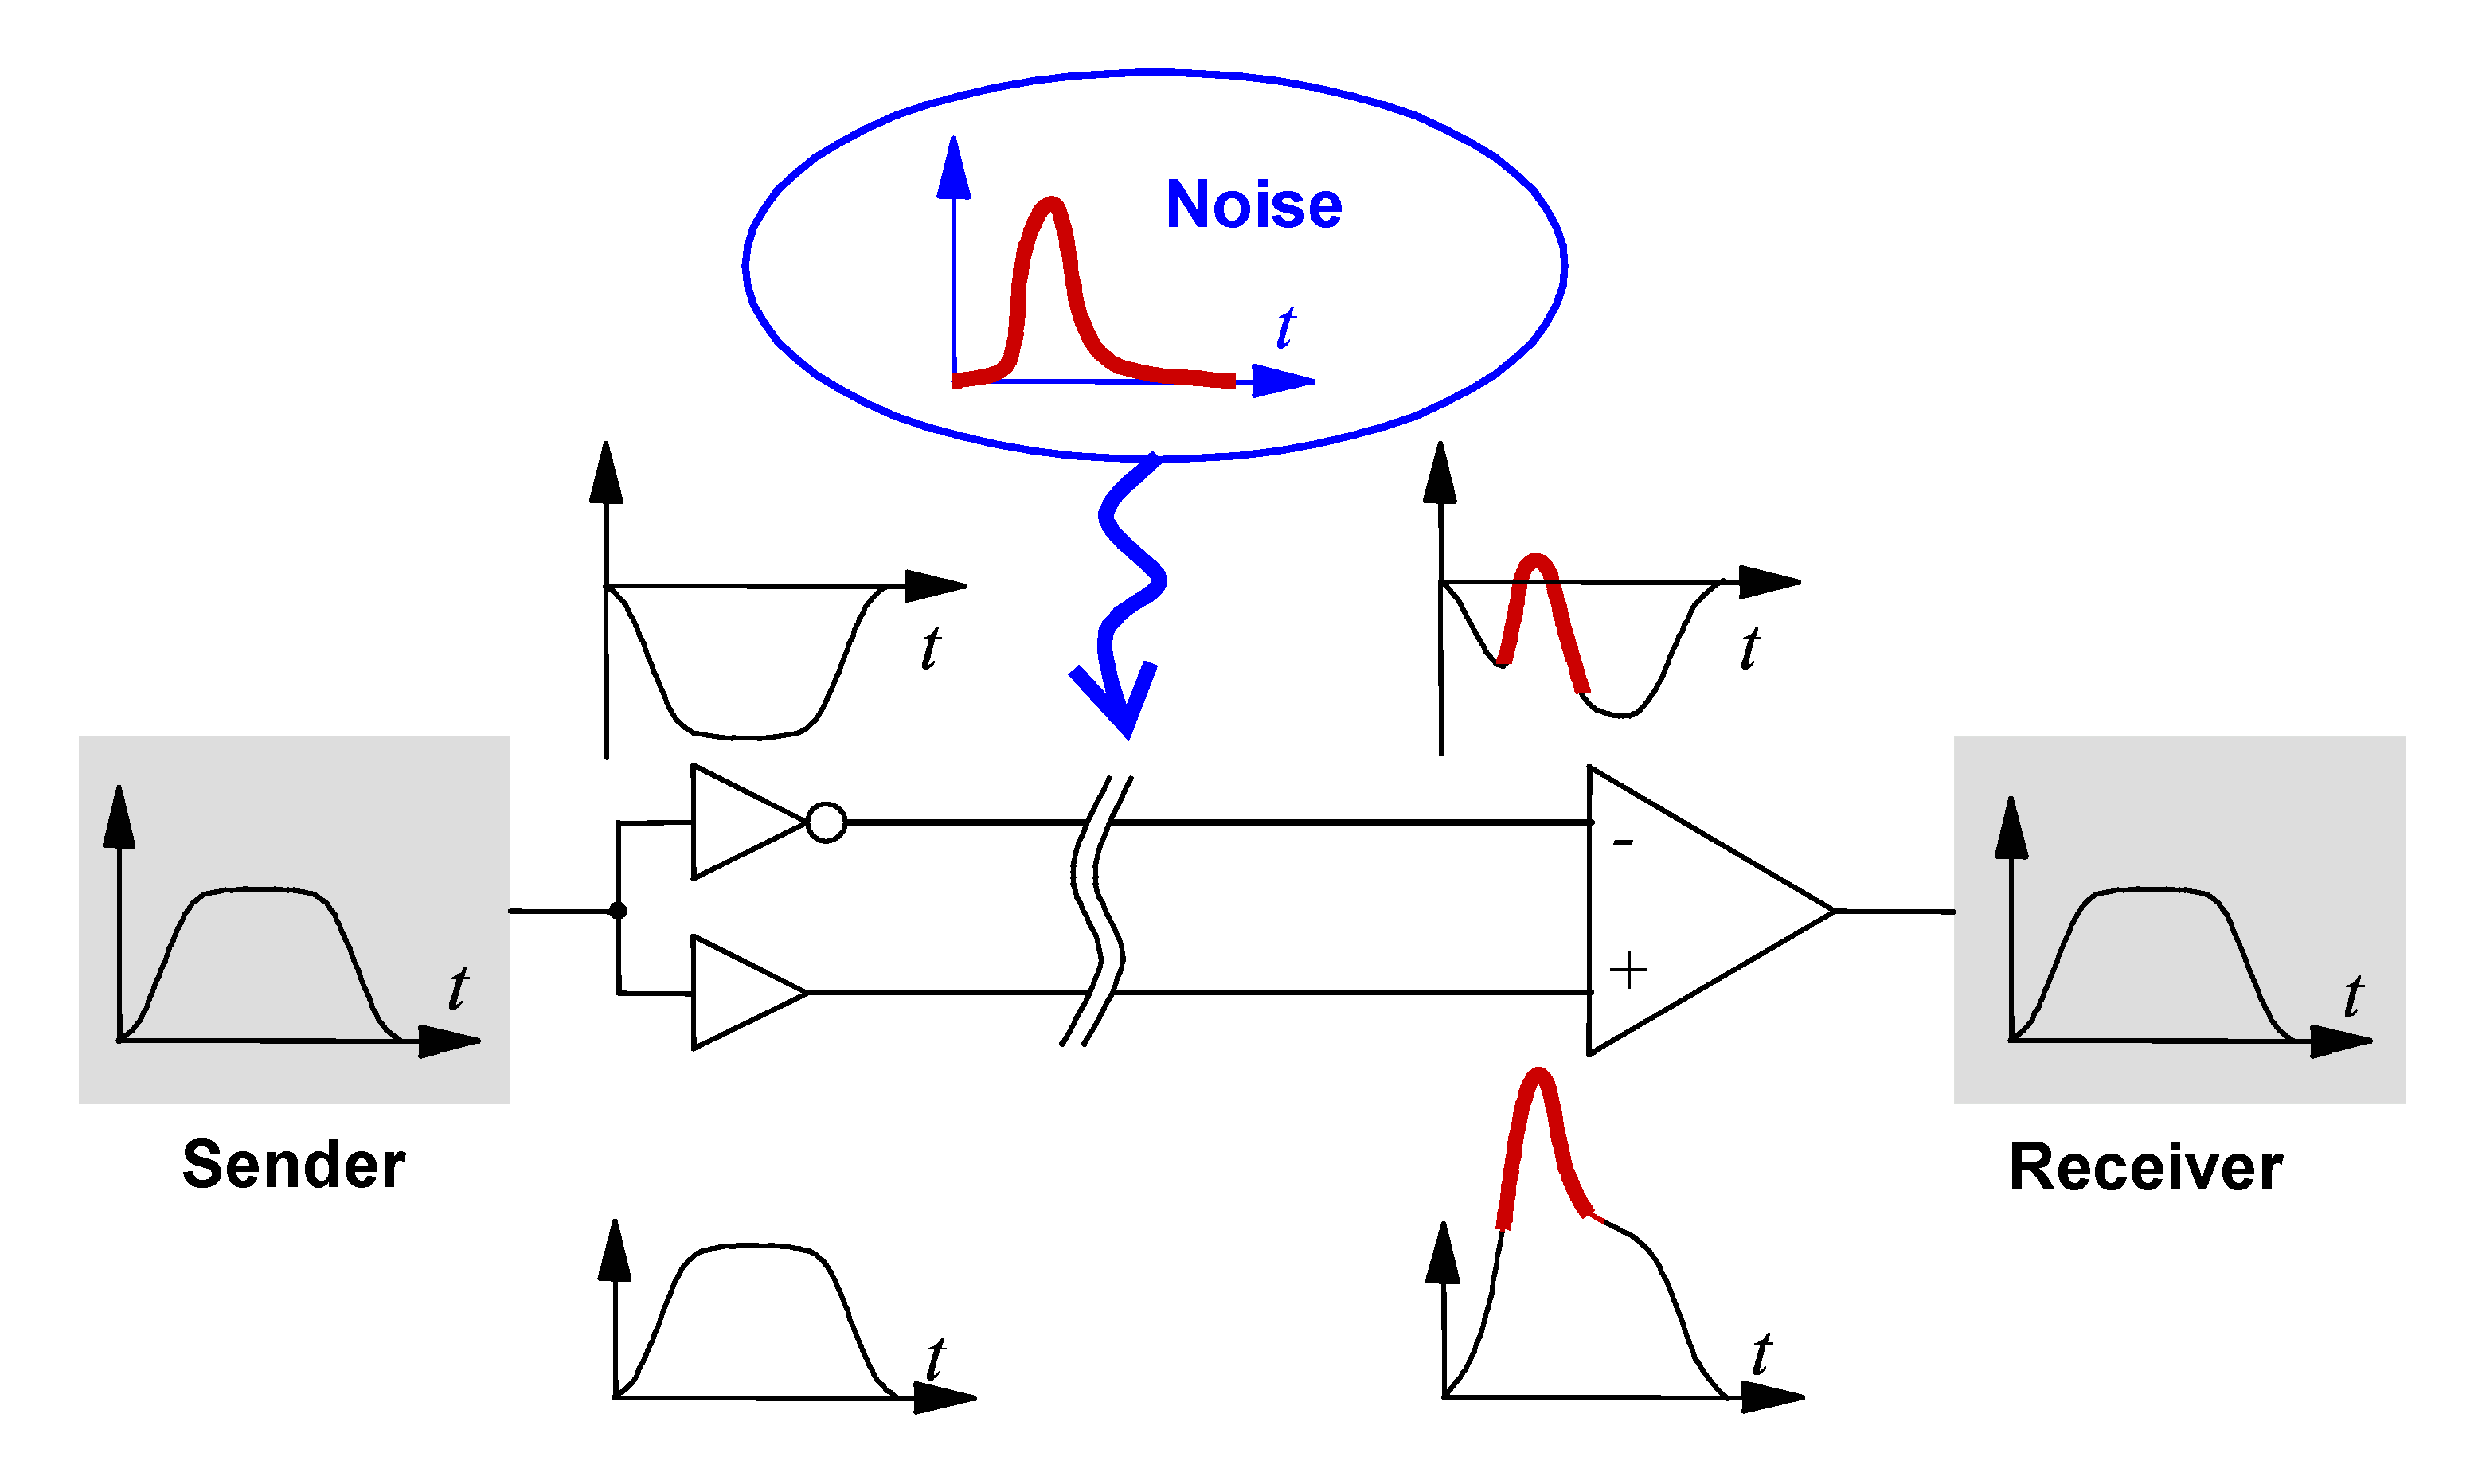
\includegraphics[width=\textwidth]{electronics/DiffSignaling}
	\caption{Noise reduction using differential signalling.~\cite{diff_signal}}
	\label{fig:electronics_diff-signal}
\end{figure}

For conventional single-ended signalling, the signal is measured as the voltage or current difference between a signal conductor and a ground common to the signal source and the signal sink.
Using a common ground as signal return path can have several undesired effects.
To shield the signal conductor, it is usually enclosed in a ground shield.
If the latter is connected on both sides, a ground loop can result for instance in combination with a shared power supply ground.
Ground loops can pick up noise through induction if the resistance along the loop is high enough.
A second way to couple noise into a single-ended system is by shifting the potential on the common ground away from the reference voltage or current, for instance due to high currents flowing through a lossy ground connection.
Because the signal is always measured against the common ground, it will be distorted.
In symmetric or differential signalling, the signal is not measured between a signal conductor and ground but instead between two signal conductors.
This works by putting an inverted (symmetric) waveform of the signal on a second conductor.
The signal is recovered by taking the difference between to two signal conductors.
As a result, the signal sink needs not be connected to the same ground as the signal source because the signal is independent of ground.
Ground loops can thus be avoided in the signal path.
Furthermore, the effects of noise pick-up on the signal lines is drastically reduced.
Due to the completely symmetric signal path, inductive noise pick-up is equal on both signal conductors as opposed to single-ended signals where the signal path is not symmetric.
In the signal sink, the difference between the two symmetric signal conductors is formed and everything that is present on both of them, such as the inductively picked up noise, cancels out.

Disentangling the three different sources of noise (thermal noise, resonances, and external pick-up) is not easy.
Hints can often be found in the spectrum of the noise.
Thermal noise is equal and uncorrelated over the full frequency spectrum.
Resonances usually occur at specific frequencies and thus produce regular patterns such as a sine at the resonance frequency.
External sources are more difficult to identify.
If the source produces \gls{em} fields at known frequencies (e.g.\ harmonics of a switched power supply) the noise spectrum can be scanned for these.
On the other hand if the source is unknown, debugging is much more complex.


\subsection{\AT{} Chain}
\label{sec:studies_electronics_at}

Contemporary electronics schemes shall be introduced by looking at the existing readout chain at LHEP at the University of Bern.
It was originally designed for the \AT{} experiment and a more detailed description can be found in~\cite{AT_larasic}.

The charge collected by the readout plane is amplified by LARASIC4*~\cite{larasic} cryogenic charge amplifiers developed by \gls{bnl} for \uboone{}~\cite{uboone}.
A performance characterisation of these \glspl{asic} can be found in~\cite{AT_larasic}.
Their main features include

\begin{itemize}
	\item \num{16} channels per \gls{asic};
	\item low noise charge amplifiers incorporating high-order filters;
	\item per channel programmable gain of \SIlist[list-final-separator = { or }]{4.7; 7.8; 14; 25}{\milli\volt\per\femto\coulomb};
	\item per channel programmable filter peaking time of \SIlist[list-final-separator = { or }]{0.5; 1.0; 2.0; 3.0}{\micro\second};
	\item built-in test capacitance connected to dedicated external test pulse input for calibration;
	\item and a power dissipation \SI{< 10}{\milli\watt} per channel.
\end{itemize}

\begin{figure}[htb]
	\centering
	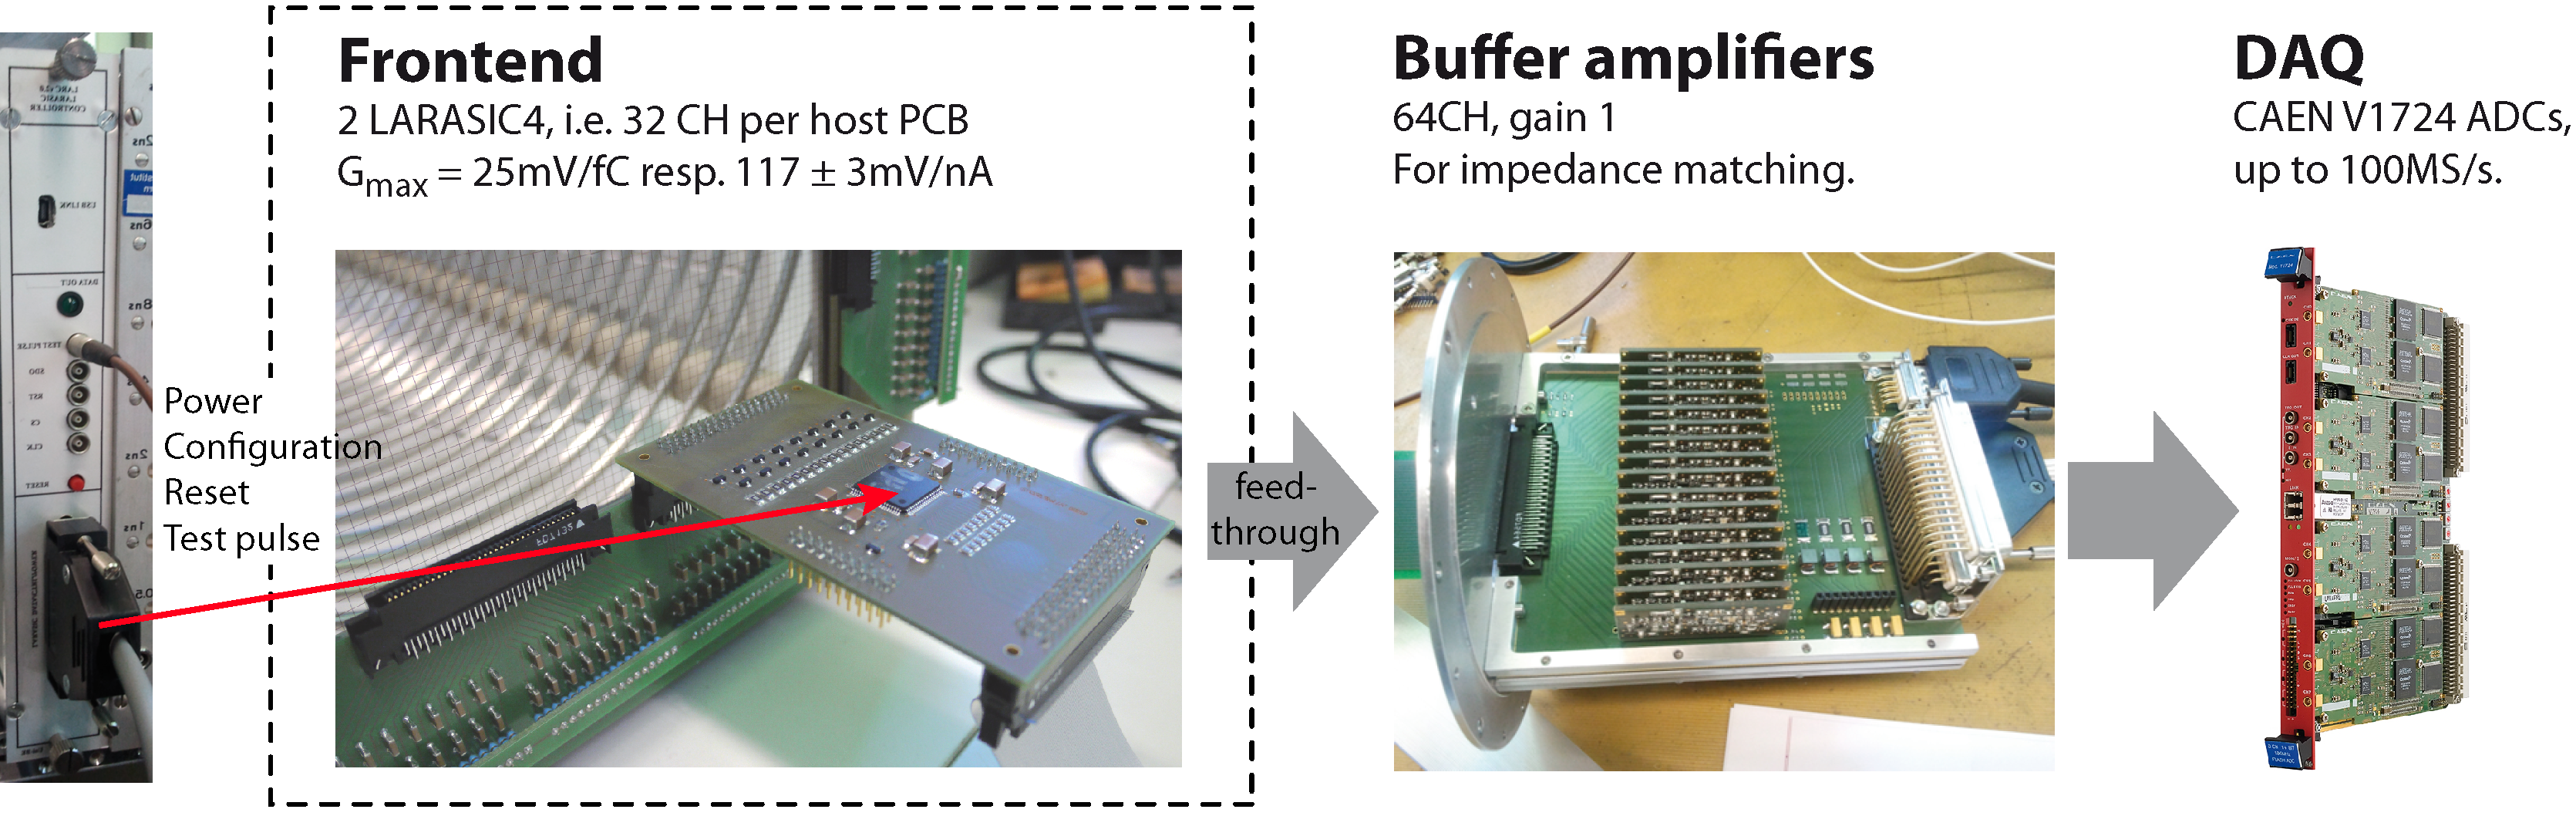
\includegraphics[width=\textwidth]{electronics/ReadoutChain_AT}
	\caption{Readout chain used for the pixel test.
		The picture of the LARASIC cryogenic front-end preamplifiers shows them installed in the \AT{} wire readout setup.~\cite{AT_larasic}}
	\label{fig:viper_readoutChain_AT}
\end{figure}

The cryogenic preamplifiers are mounted as close as possible to the readout in order to minimise noise pick-up on these very sensitive lines.
Via an \gls{i2c} bus, LARASICs can be programmed to the different aforementioned configurations.
For this purpose, they are connected to a bespoke \gls{nim} module housing an Arduino which generates the \gls{i2c} signals, a test pulse generator, and multiple low-noise voltage regulators providing power to the LARASICs.
The output of the preamplifiers is fed to buffer amplifiers mounted on top of the signal feedthrough by means of flexible Kapton ribbon cables.
The buffers operate at room temperature, have a unity gain, and match the output impedance of the LARASICs to the \SI{50}{\ohm} input impedance of the downstream digitisers.
From the buffers, the signals are routed via \SI{50}{\ohm} unbalanced coaxial lines to \emph{CAEN V1724}\footnote{\url{http://www.caen.it}} \SI{14}{bit} digitisers mounted in a \gls{vme} crate.
For debugging purposes, the output of the buffers can be routed to an oscilloscope via a coaxial T-piece.
Finally, the digital data is read out from the \gls{vme} crate via a fibre-optic link by a standard PC.
Figure~\ref{fig:viper_readoutChain_AT} depicts the entire readout chain.
The complete analogue signal path from the pixel plane to the \gls{vme} digitisers is single-ended and thus prone to ground loops and all associated noise problems.

\begin{figure}[htb]
	\centering
	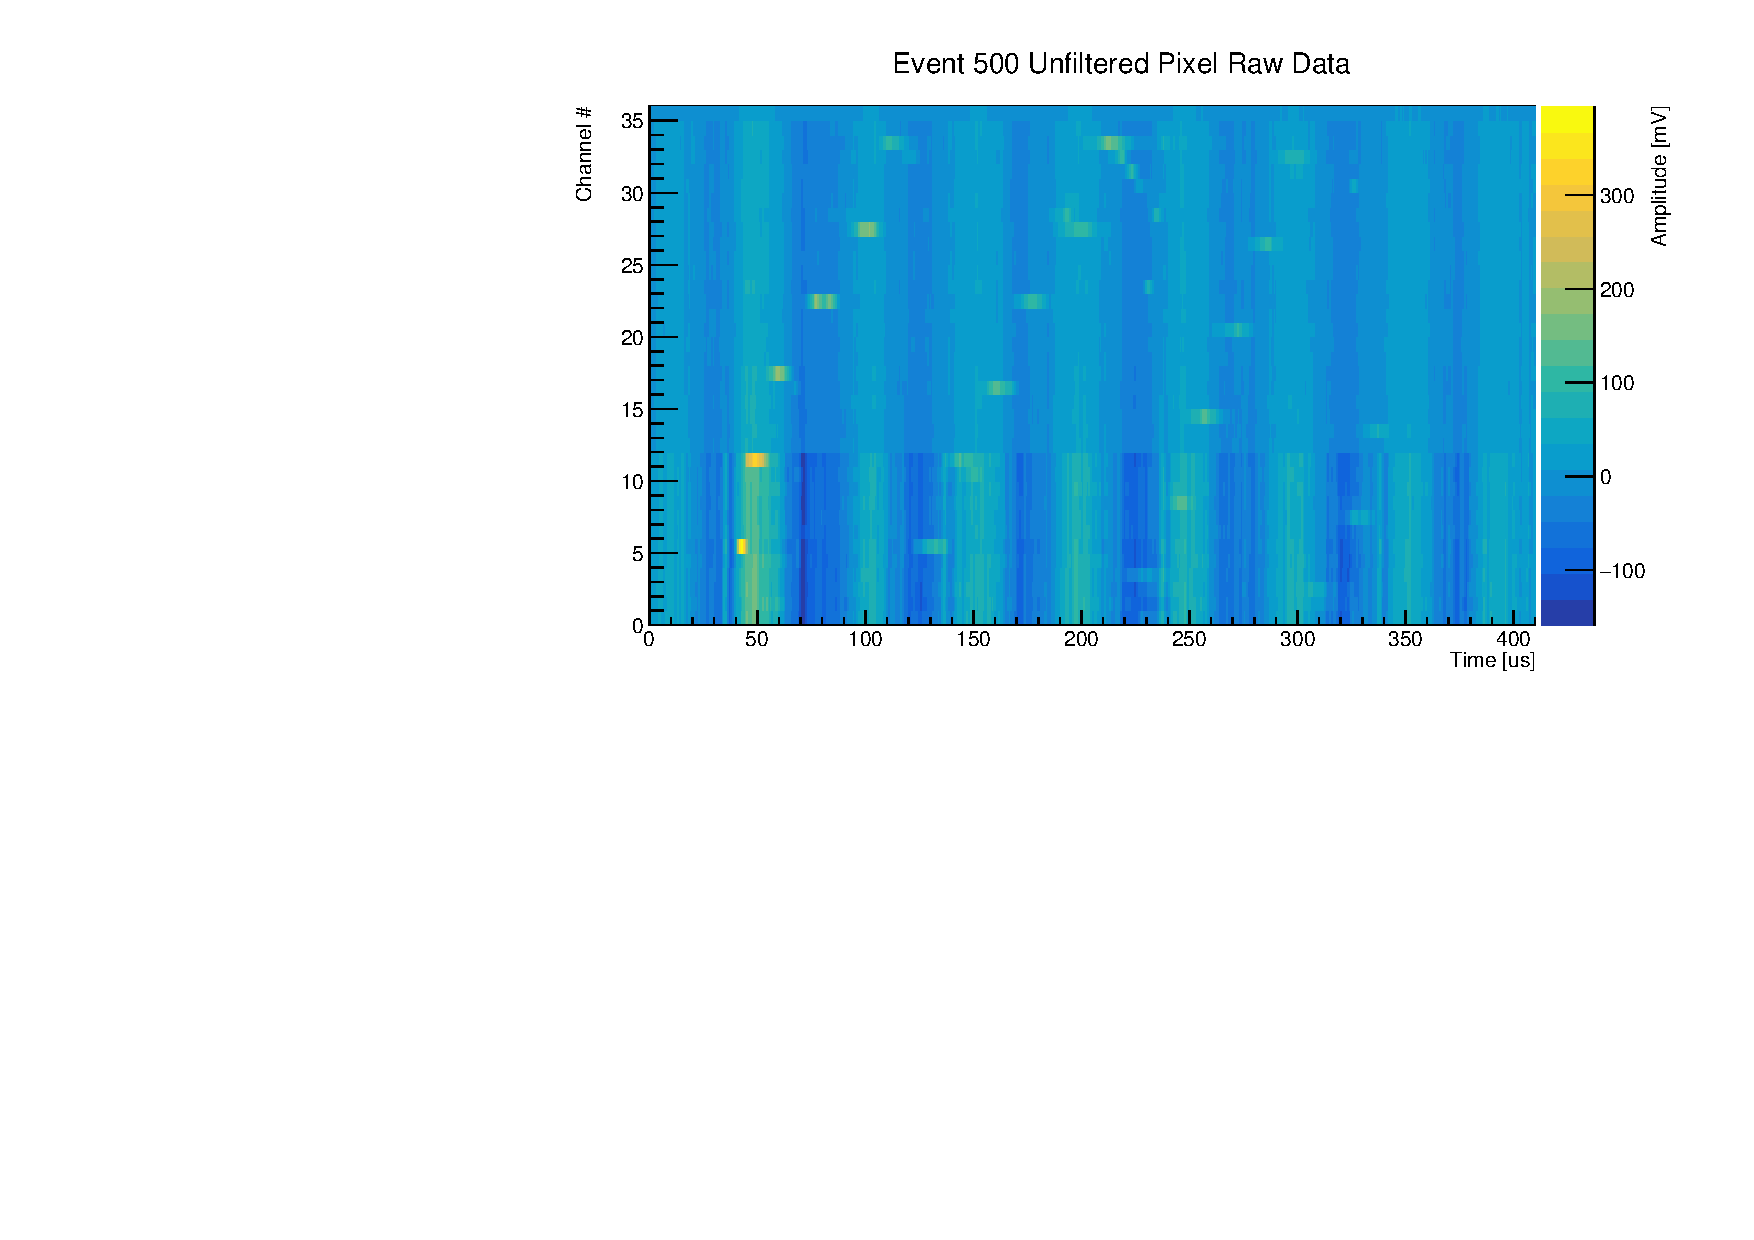
\includegraphics[width=\textwidth]{noise/event500_rawUnfilteredPixel}\\
	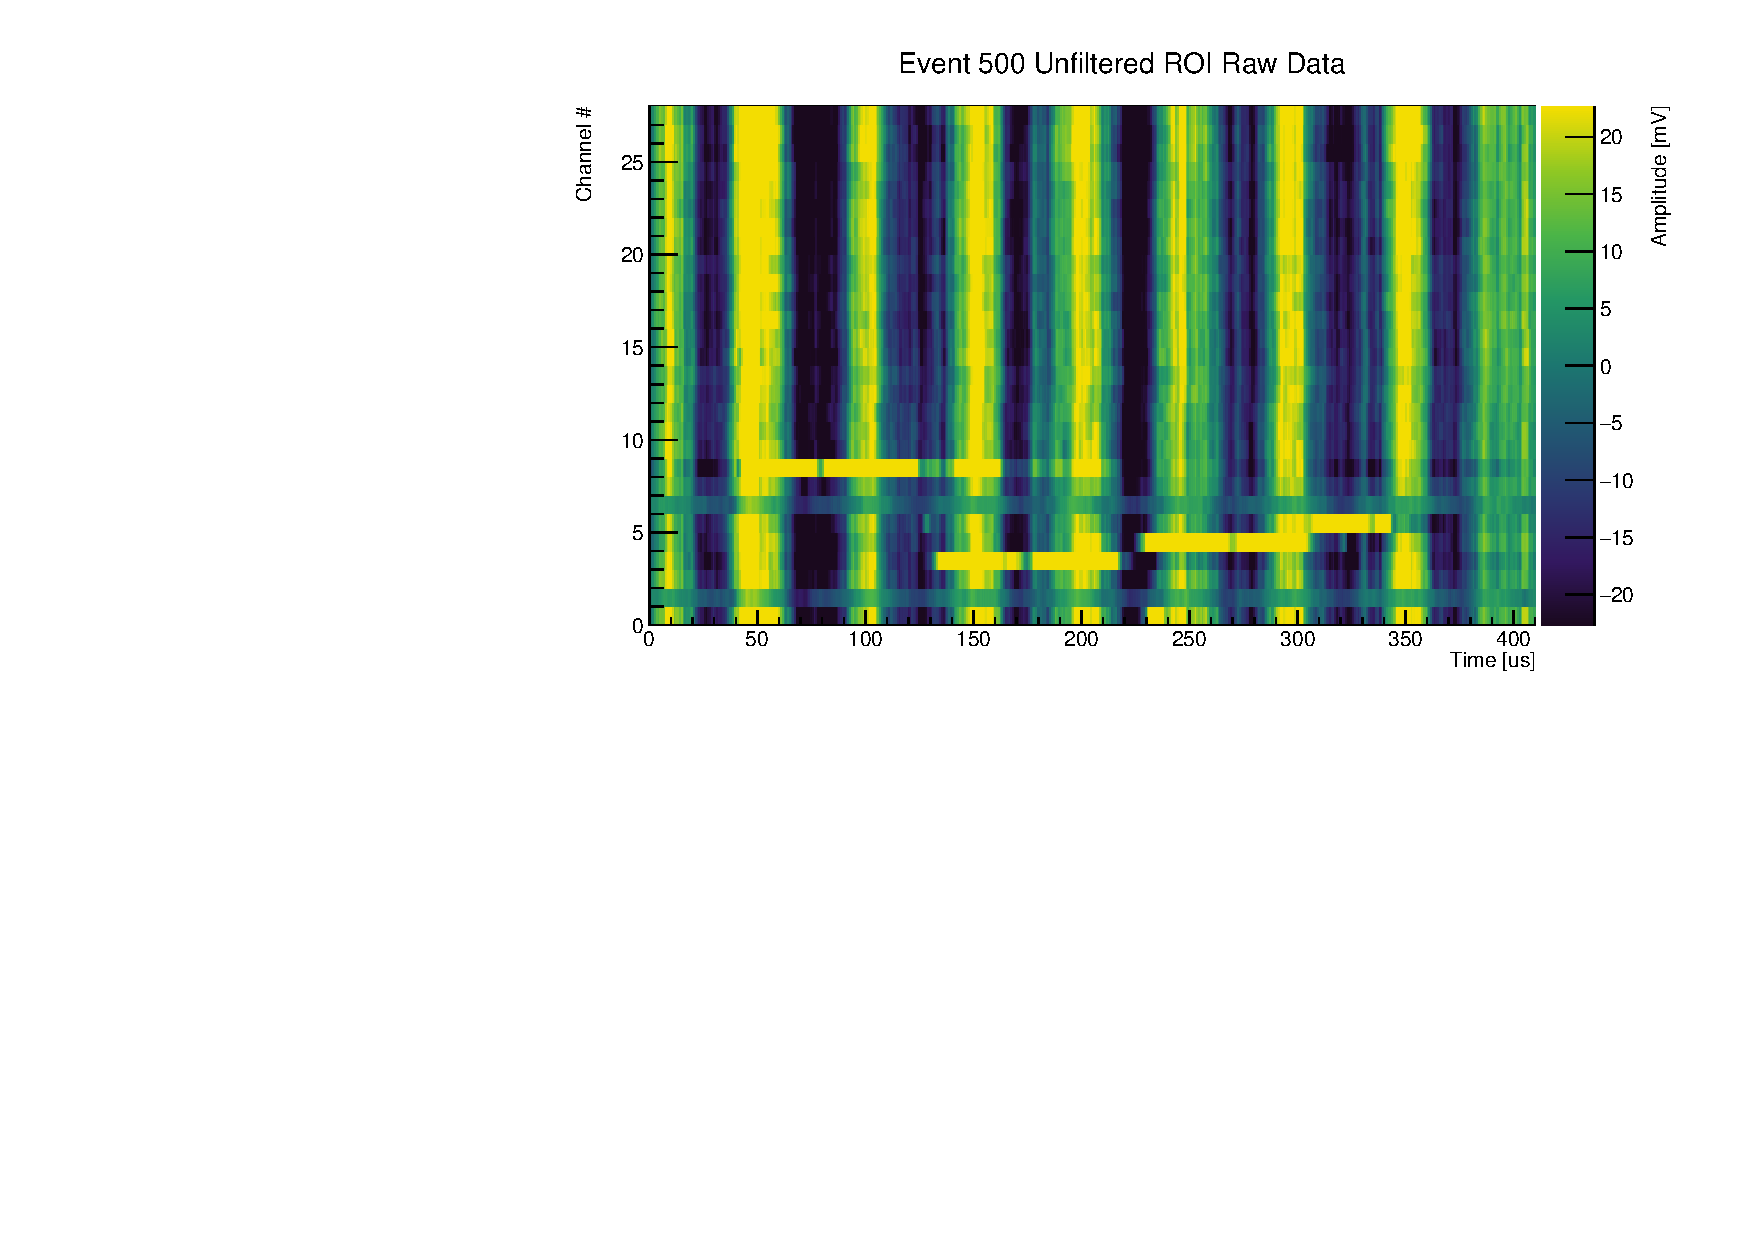
\includegraphics[width=\textwidth]{noise/event500_rawUnfilteredROI}
	\caption{Event from the first measurement campaign of the pixel prototype.
	The top plot shows pixel data while the bottom plot shows \gls{roi} data.}
	\label{fig:electronics_event-run1}
\end{figure}

During the first pixelated readout measurement campaign (see Sections~\ref{sec:studies_charge-ro} and~\ref{sec:ac_viper}), it became apparent that the data was significantly impaired by noise.
As can be seen in Figure~\ref{fig:electronics_event-run1}, the noise amplitude is similar over multiple channels.
This implies a common mode component that cannot originate from inductive pick-up.
Instead, the noise is likely generated by self-oscillating parts of the signal path due to ground loops and parasitic impedances.
For the second measurement campaign, different steps were take to mitigate this behaviour through modifications to detector location, power supply, signal path, and intrinsic capacitance.

A correlation between noise levels and the running state of the air condition in the utility room next to the lab was found.
Therefore, the experimental setup was moved away from the wall facing the utility room.

A decoupled clean power grid was built in the lab.
A Motor Generator (M-G set) separates the lab grid mechanically from the building power supply.
Thus, any noise present on the latter is prevented from entering the experimental setup.
Furthermore, this decouples the lab grid entirely from the building ground preventing ground loops via electric mains.

\begin{figure}[htb]
	\centering
	\includegraphics[page=4, width=\textwidth]{noise/noise_run1} \\
	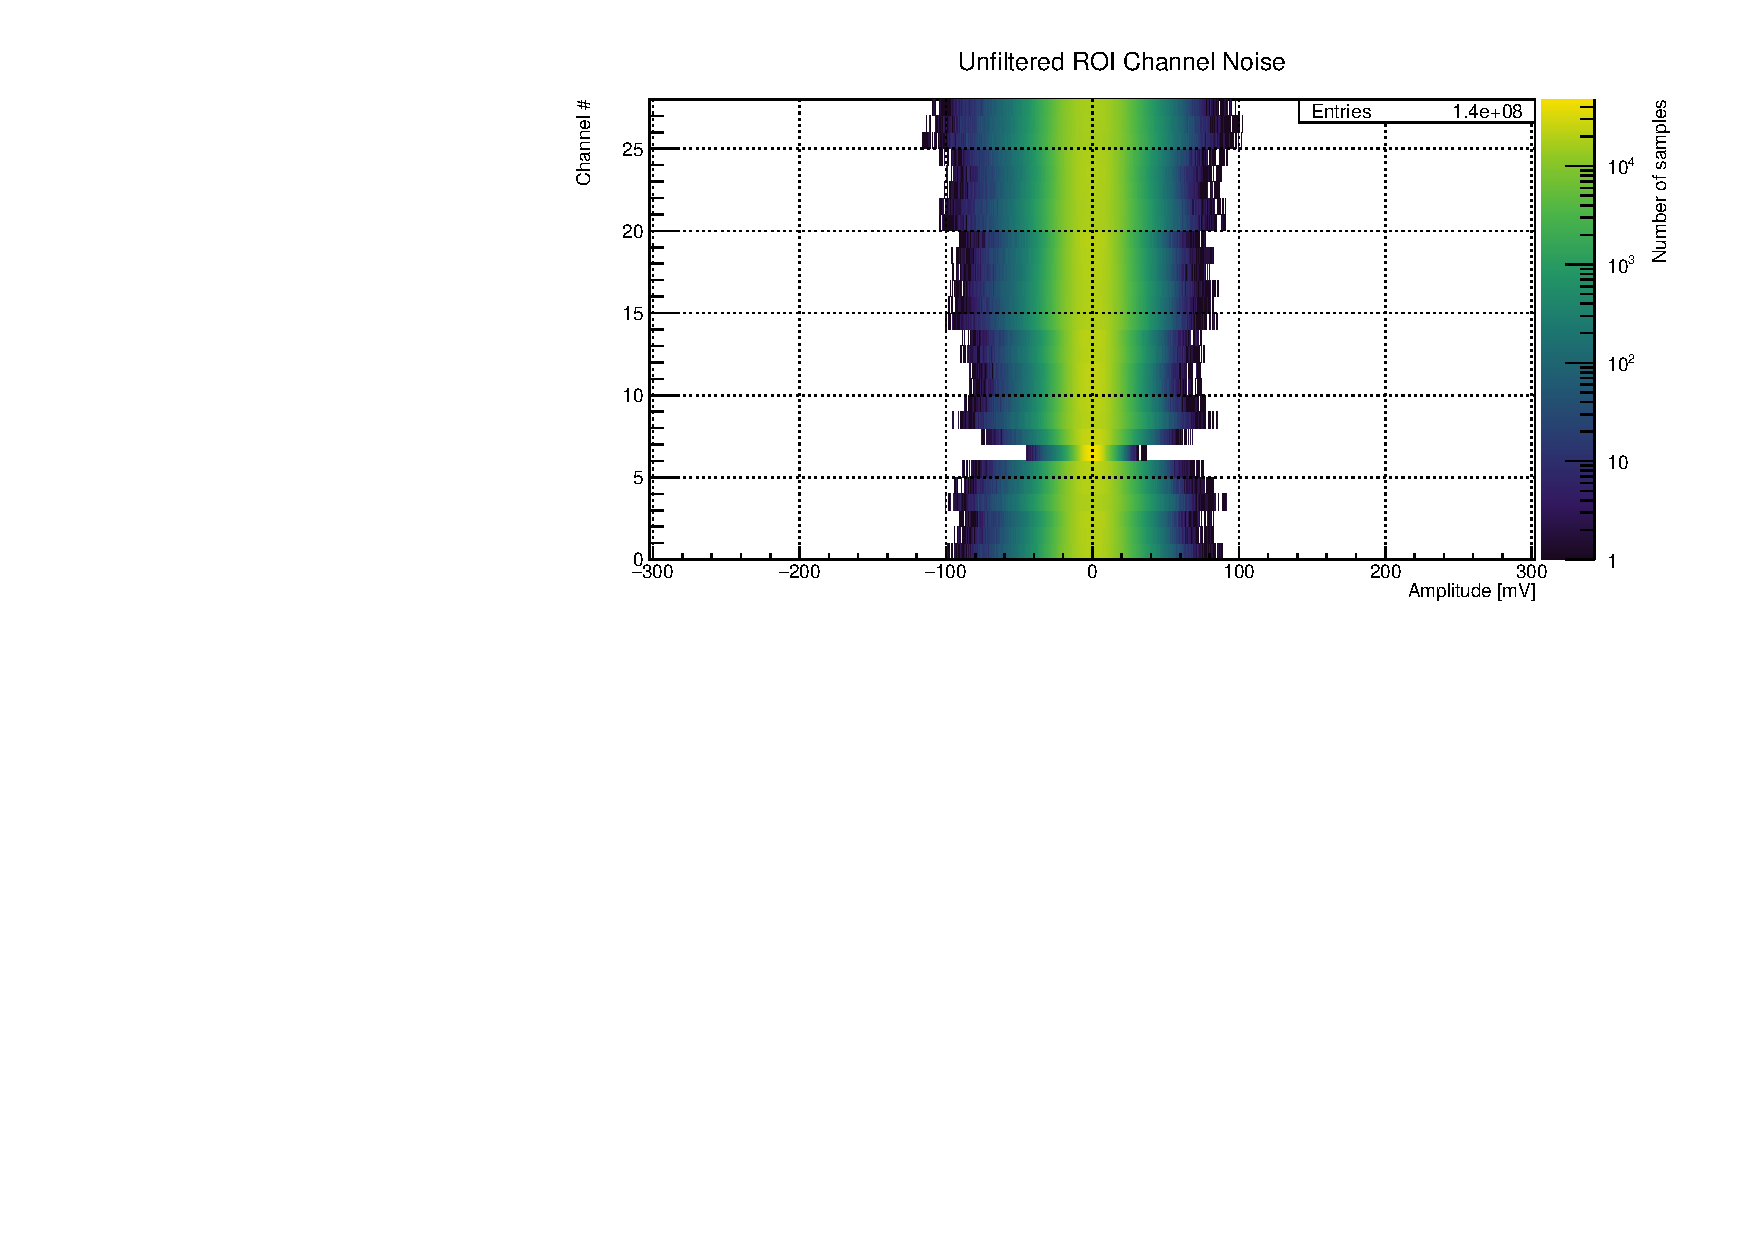
\includegraphics[page=1, width=\textwidth]{noise/noise_run1}
	\caption{Noise amplitude distributions of pixel (top) and \gls{roi} (bottom) channels of the first measurement campaign.
	\num{5000} events with \num{1000} \SI{410}{\nano\second} samples each from a \SI{5}{\hertz} random trigger were combined.}
	\label{fig:electronics_noise-run1}
\end{figure}

The signal path from the impedance-matching buffer amplifiers to the digitisers---i.e. the warm signal path---was changed from single-ended to differential signalling.
This was achieved by replacing the buffer amplifiers by single-ended to differential amplifiers and inserting another stage upstream of the digitisers to change the signal back to \SI{50}{\ohm} single-ended, matching the input of the digitisers.
Like this, noise pick-up outside the cryostat could be reduced as well as sensitivity to ground loops between the detector and the \gls{daq} rack.
The design for the two buffer stages was kindly provided by the \lariat{} collaboration (see Section~\ref{sec:ac_pixlar} and~\cite{lariat}).

\begin{figure}[htb]
	\centering
	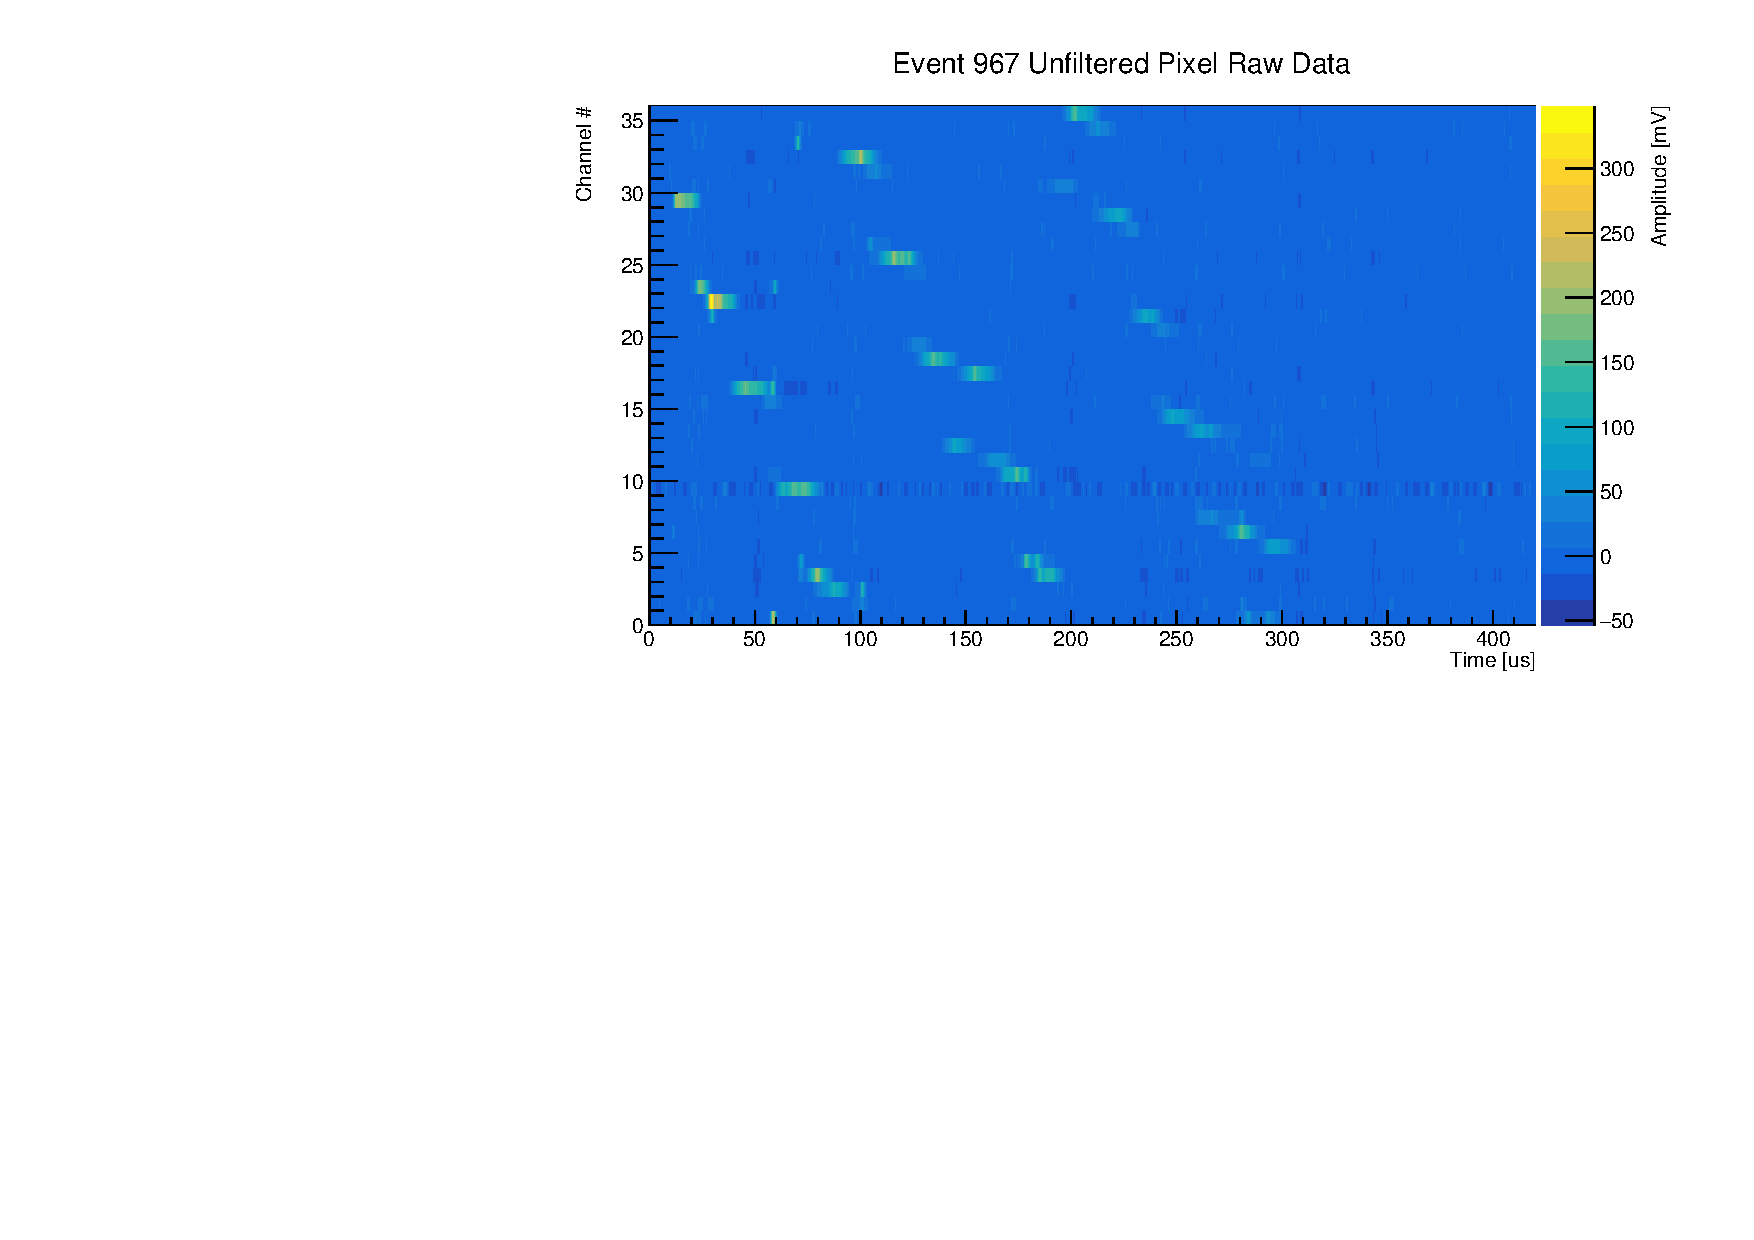
\includegraphics[width=\textwidth]{viper/event967_rawUnfilteredPixel}\\
	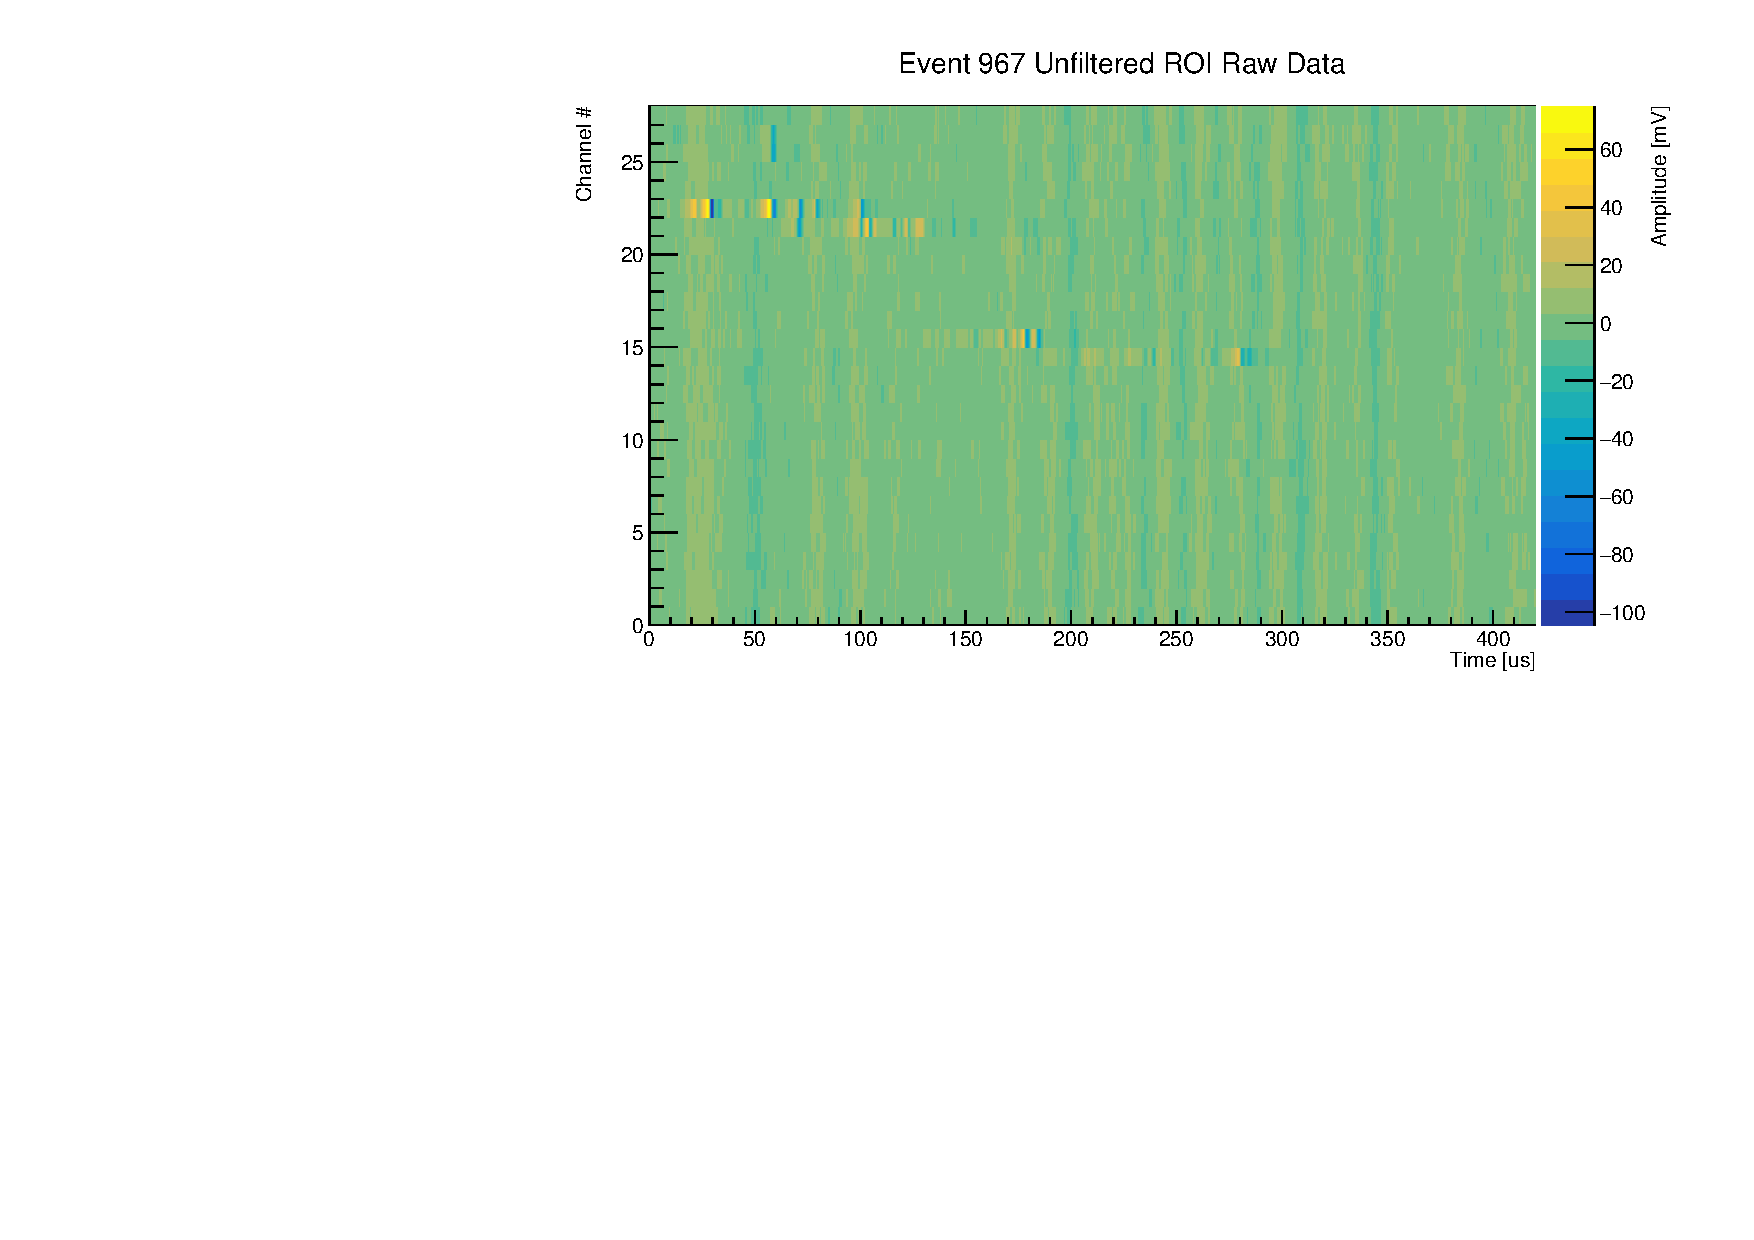
\includegraphics[width=\textwidth]{viper/event967_rawUnfilteredROI}
	\caption{Event from the second measurement campaign of the pixel prototype after improving the readout chain.
	The top plot shows pixel data while the bottom plot shows \gls{roi} data.}
	\label{fig:electronics_event-run2}
\end{figure}

A source of noise was identified in the layout of the pixel readout plane.
It was found that due to several ground planes and long tracks in the \gls{pcb}, parasitic capacitances are very high.
Pixel channels are affected particularly due to the increased total track lengths from connecting multiple pixels to the same \gls{daq} channel.
This is problematic because for high enough frequencies---determined by $RC$---, the input is shorted to ground creating a ground loop again.
Through this capacitive coupling to ground, the system can start to oscillate.
One evidence for this is that the noise is equal over multiple channels, so-called common-mode noise.
More specifically, the noise is equal for two respective groups of channels (see Figure~\ref{fig:electronics_event-run1}).
Investigating this, it was found that these groups correspond to channels of roughly equal parasitic capacitance: \SI{150 +- 5}{\pico\farad} and \SI{95 +- 5}{\pico\farad}.
The noise amplitude is higher on channels with higher capacitance (see Figure~\ref{fig:electronics_noise-run1}).
To solve this problem, the \gls{pcb} design was optimised by removing unnecessary ground planes, routing signal tracks outside necessary ground planes and increasing the thickness of the \gls{pcb}.
Pixel capacitance could be improved to \SI{65 +- 5}{\pico\farad} for all channels.
\gls{roi} capacitance improved only slightly from \SI{25 +- 10}{\pico\farad} to \SI{20 +- 10}{\pico\farad} which confirms the hypothesis that the long tracks due to pixel multiplexing were the culprits.
The reason for the higher spread of the \gls{roi} capacitances is the larger difference in track length between the different \glspl{roi}.
For the sake of completeness, it should be noted here that for the capacitance measurements, the old \gls{pcb} was not populated while the new one was populated as described in Section~\ref{sec:ac_viper_pcb}.
However, the installed capacitors are either not connected to ground or in series with a \SI{10}{\mega\ohm} resistor.
Therefore, their influence on the measurements is negligible.

As can be seen from Figures~\ref{fig:electronics_event-run1} and~\ref{fig:electronics_event-run2}, there is a significant decrease in noise after commissioning all of the above improvements to the readout chain.
This can also be seen from Figures~\ref{fig:electronics_noise-run1} and~\ref{fig:electronics_noise-run2} depicting the noise amplitude distribution of the two measurement campaigns.
The data for the latter (\num{5000} events in the first and \num{2000} events in the second campaign) was taken employing a \SI{5}{\hertz} random trigger.
A more detailed assessment of the noise after the implementation of the described noise mitigation measures can be found in Section~\ref{sec:ac_viper_snr}.

\begin{figure}[htb]
	\centering
	\includegraphics[page=4, width=\textwidth]{noise/noise_run2} \\
	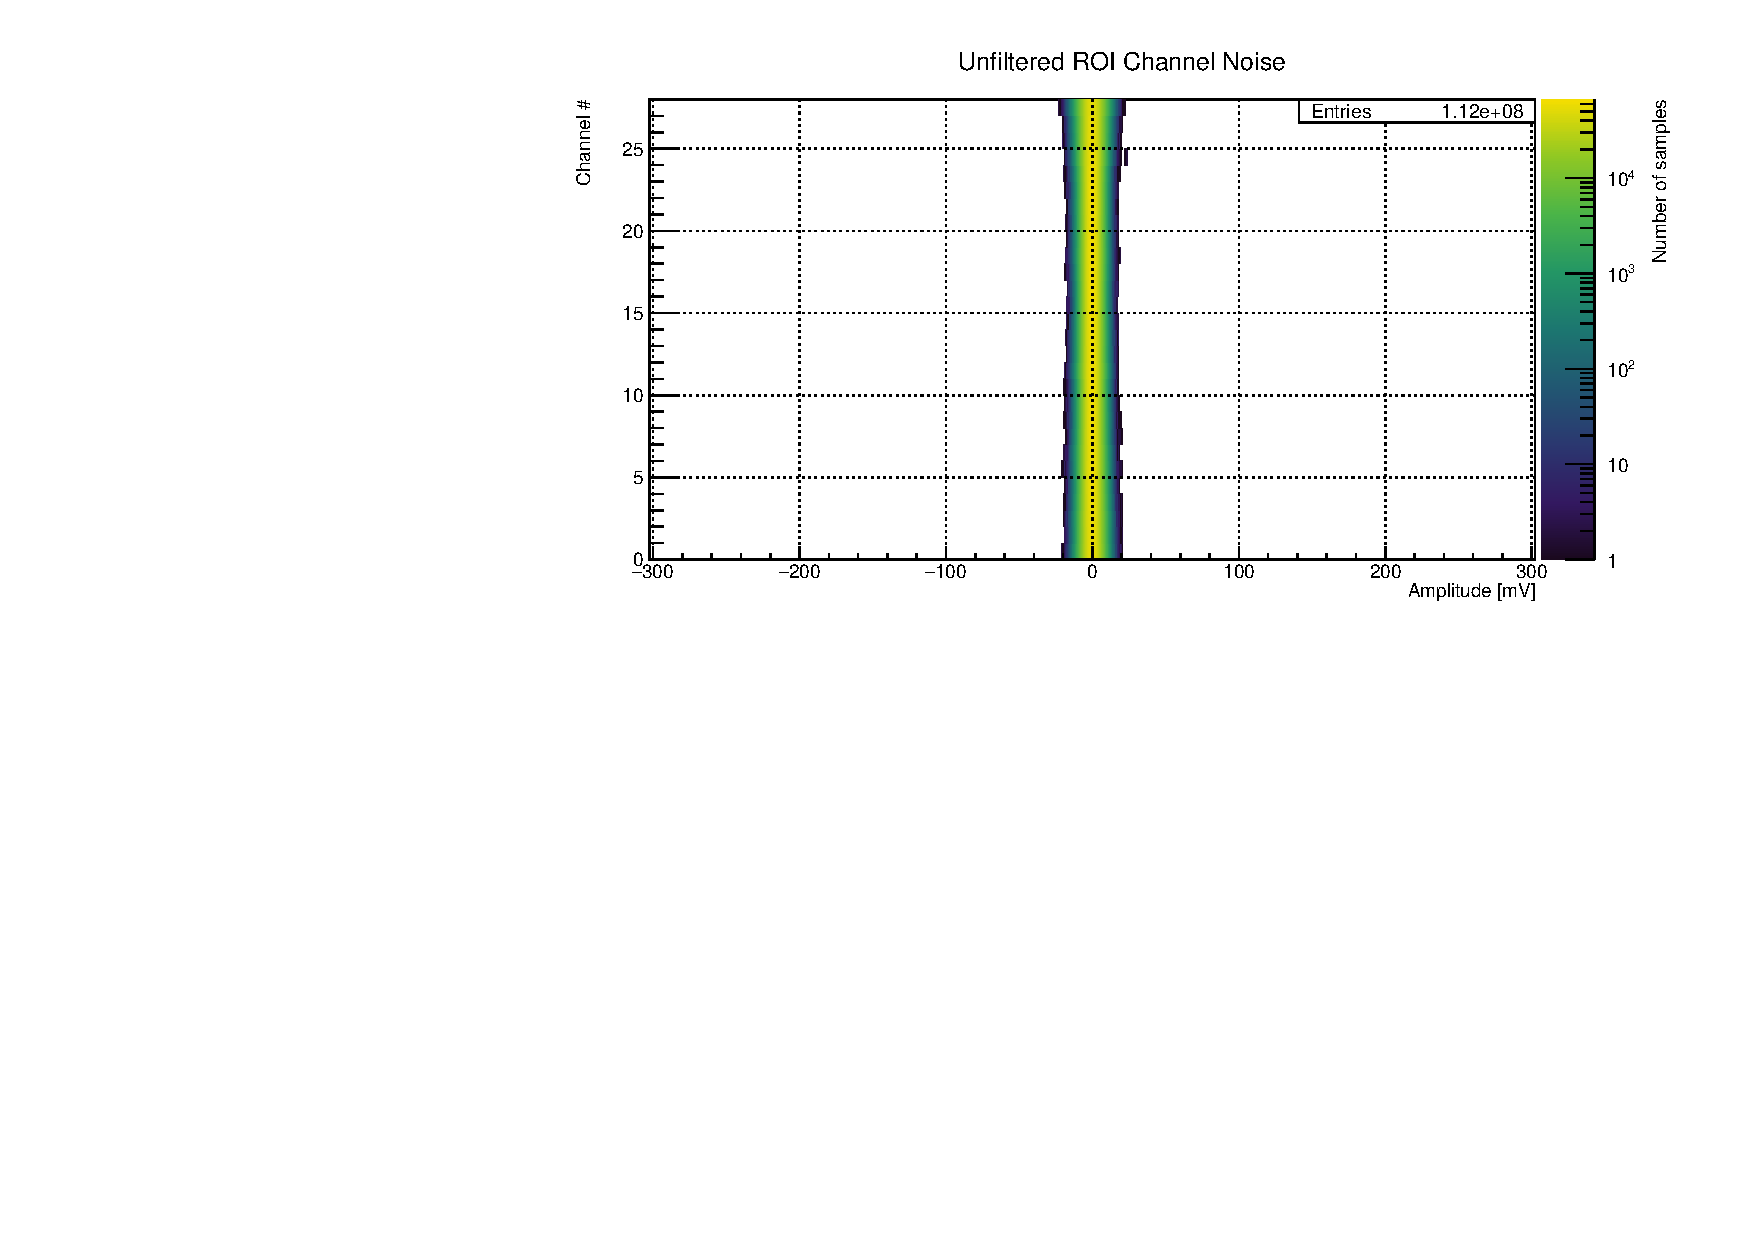
\includegraphics[page=1, width=\textwidth]{noise/noise_run2}
	\caption{Noise amplitude distributions of pixel (top) and \gls{roi} (bottom) channels of the second measurement campaign, after implementing hardware noise mitigation measures.
	\num{2000} events with \num{2000} \SI{210}{\nano\second} samples each from a \SI{5}{\hertz} random trigger were combined.}
	\label{fig:electronics_noise-run2}
\end{figure}


\subsection{Improved Cold Electronics for Pixelated Readouts}
\label{sec:studies_electronics_pixel}

This section describes the challenges met by electronics for pixelated \lartpc{}s and possible solutions.
First, the cryogenic \glspl{adc} for the \dune{} \gls{fd}, developed by \gls{bnl}, are introduced, and an explanation is given why they are unsuitable for a pixelated \gls{nd}.
Therefore, the neutrino group at \gls{lbnl} is developing bespoke pixel electronics for the \gls{nd}, called \larpix{}.
An overview of this effort is given in the second part of this section.

As mentioned in Section~\ref{sec:lartpc_electronics}, cold digitisation can improve noise because of both shorter analogue signal lines and reduced thermal noise of the electronics.
Furthermore, it enables the multiplexing of the data on high-speed digital links, reducing the number of needed signal cables and cryostat feedthroughs.
However, designing reliable electronics at cryogenic temperatures is not an easy task.
\glspl{adc} in particular are very sensitive to stable reference voltages required for proper analogue-to-digital conversion.
Another problem arises from the fact that digital electronics in general require clocks with sharp edges for proper timing, usually realised as a square wave.
According to Fourrier analysis, a square wave produces a high level of harmonics.
This is particularly problematic in case of readout wires that act as antennas and can pick up theses clock signals.
A further important aspect is power dissipation.
All power dissipated by cryogenic electronics needs to be compensated for in order to prevent the \lar{} from boiling.
This is particularly problematic for a pixelated readout that requires a much higher number of readout channels than a wire readout (see Section~\ref{sec:studies_charge-ro_pixel}).

\gls{bnl} is developing cold charge readout electronics for the \dune{} \gls{fd}.~\cite{protodune-sp}
In particular, the plan is to accompany the cryogenic LARASIC charge preamplifiers by cryogenic \glspl{adc}.
They have \num{16} inputs, each capable of digitising the \gls{tpc} signals at \SI{2}{\mega{}S\per\second} and \SI{12}{bit} with input characteristics optimised for the LARASIC output.
A more detailed description is given in~\cite{bnl_adc}.

In the course of this work, the cryogenic \gls{adc} \glspl{asic} developed by \gls{bnl} were evaluated to be used in the \gls{nd} as well.
The author joined the team at \gls{bnl} in cold tests of the devices.
One of the results of these tests is presented here to illustrate the difficulties of cryogenic \glspl{adc}.
As a disclaimer, it should be noted that this is by no means the current status of the \glspl{adc} at the time of this writing.
The described tests were performed in the Fall of 2016 at \gls{bnl}.

An important characteristic of an \gls{adc} is linearity.
It describes the relation between the applied input voltage and the calculated digital number, the \emph{\gls{adc} code}, at the output.
In the case of the \gls{bnl} \glspl{adc}, this relation is expected to be strictly linear.
To test this, a voltage ramp is applied to the input and the converted digital values are recorded.

\begin{figure}[htb]
	\centering
	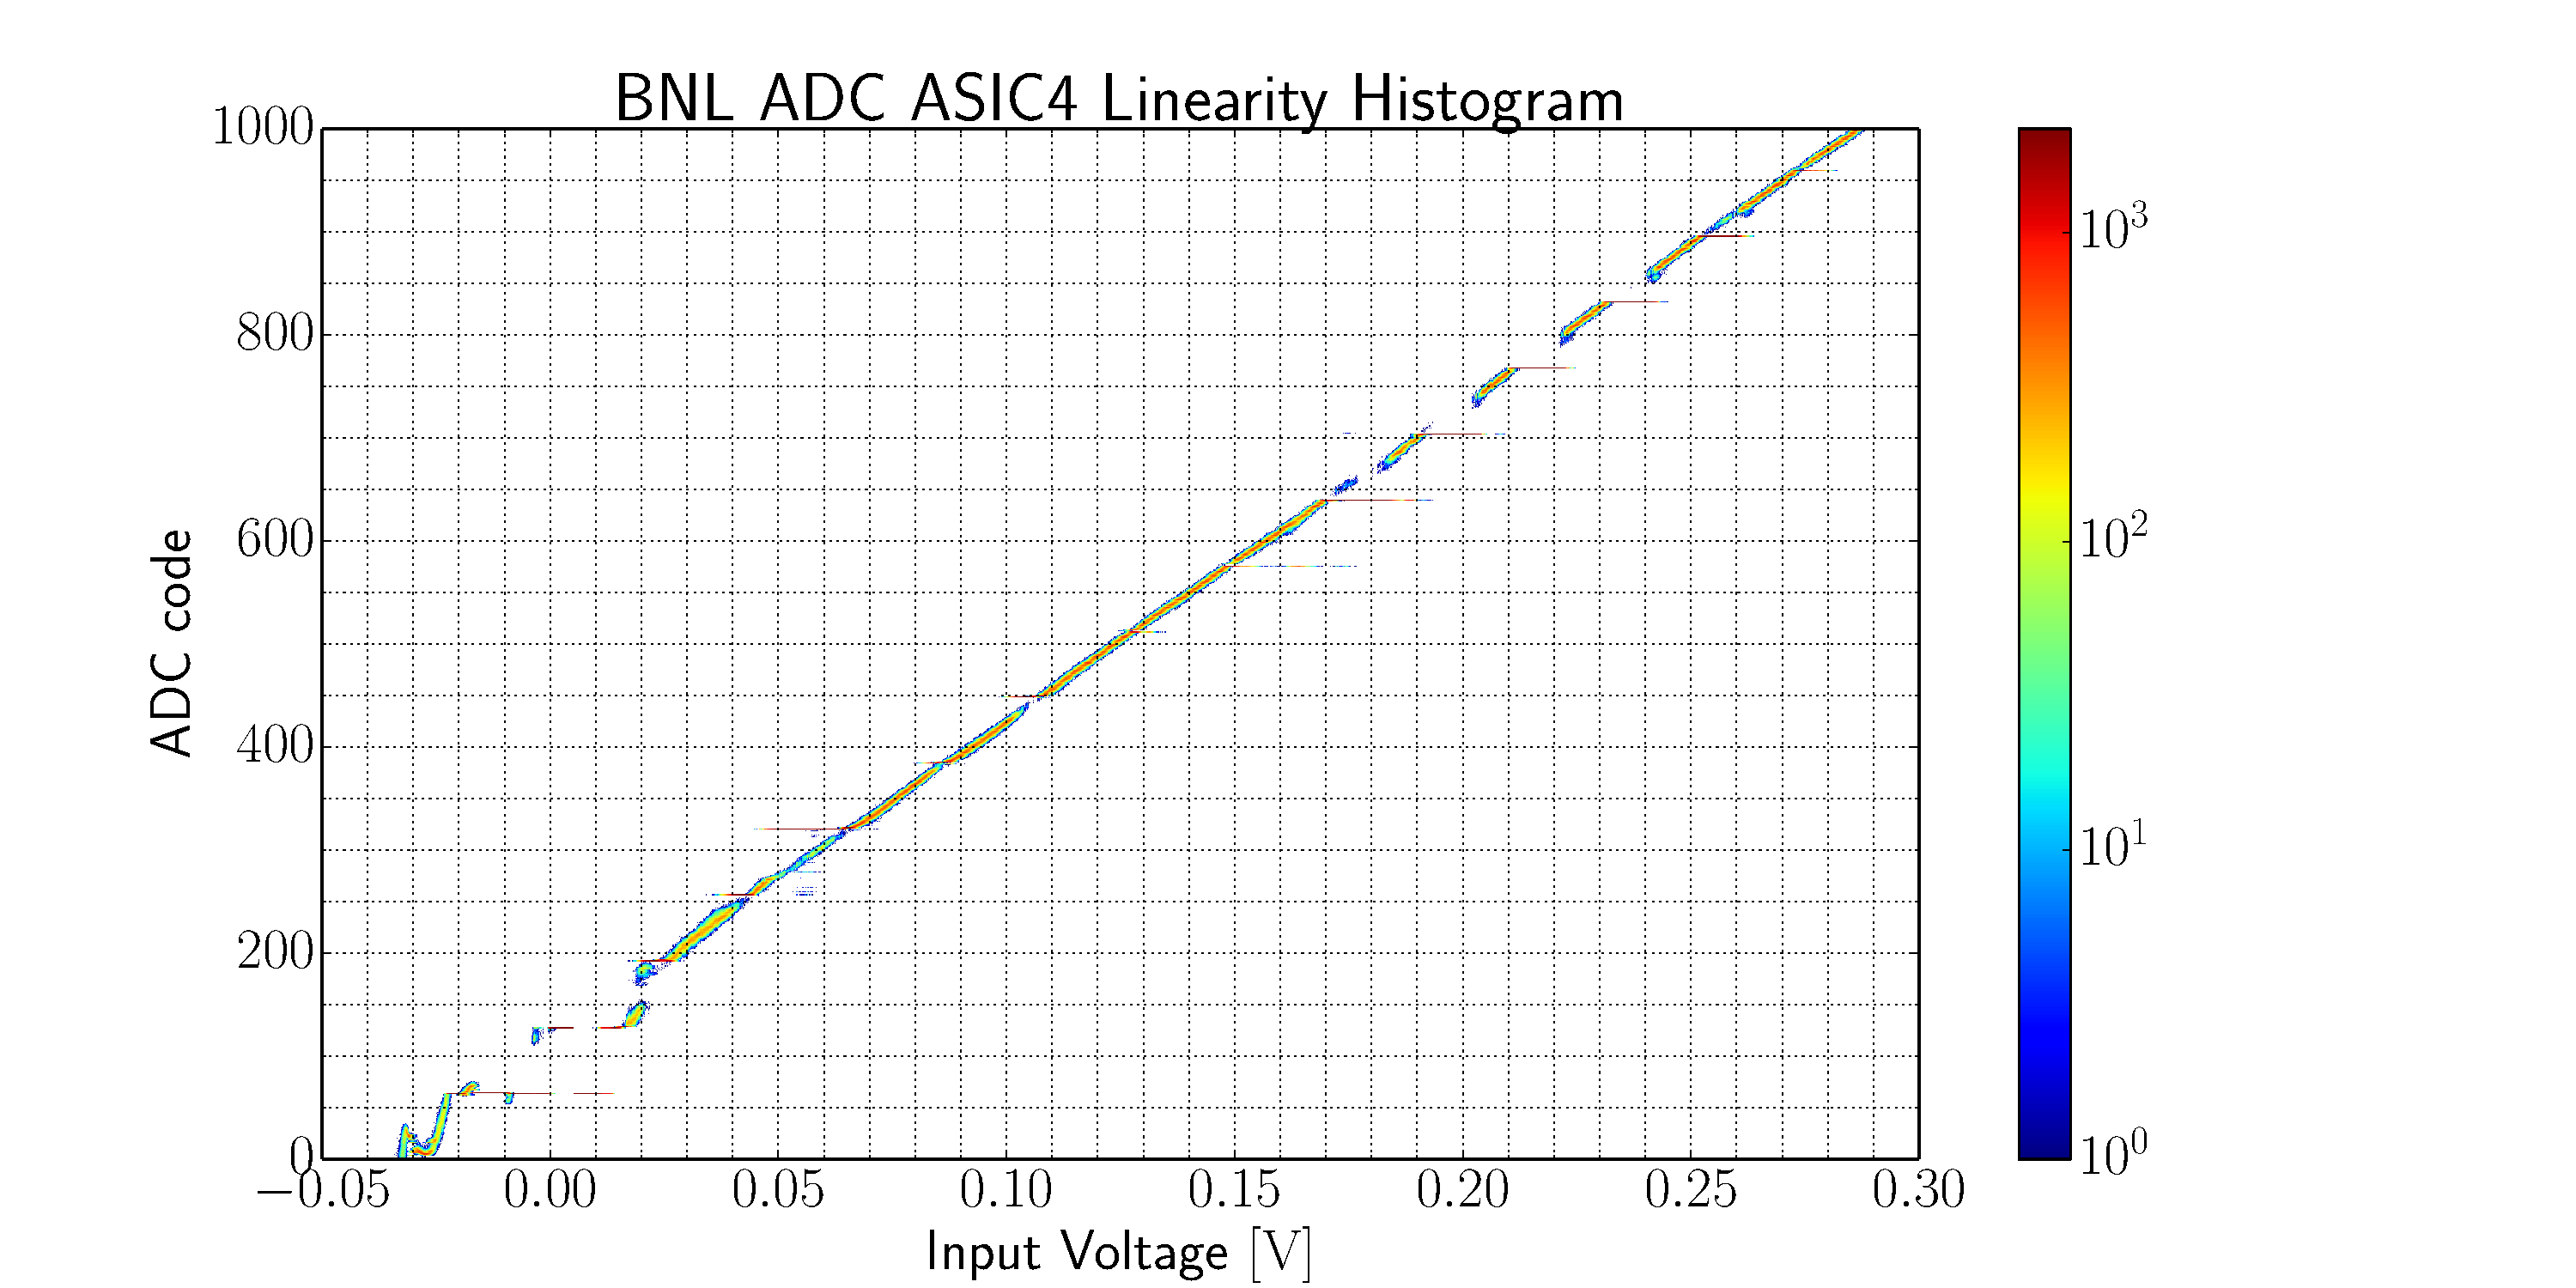
\includegraphics[width=\textwidth]{bnl/bnl_adc_lin}
	\caption{Linearity measurement of the \gls{bnl} cryogenic \gls{adc} \glspl{asic} with input voltage on the x-axis and \gls{adc} value (code) on the y-axis.
	Color represents the number of measurements.
	The measurements were performed in liquid nitrogen.}
	\label{fig:bnl_adc_lin}
\end{figure}

A typical measurement is shown in Figure~\ref{fig:bnl_adc_lin}.
The expected shape is one straight diagonal line from the bottom left to the top right corner, i.e.\ a linear relationship between input voltage and \gls{adc} value.
Two particular deviations from this are visible: gaps accompanied by horizontal lines and a wobbly response around zero.
Upon close inspection, it can be seen that the gaps have the same voltage range as the horizontal lines.
The meaning of this is that for this input voltage range, the \gls{adc} output is \emph{stuck} at the same value.
Both these effects mean that the detector response to detected charge and thus energy deposition is not linear.
While some non-linearities can be compensated in offline data analysis, this is not possible for the sticking \gls{adc} values because they correspond to a range of input voltages.
This impairs the energy resolution of the detector.

The cause for the non-linearities is rooted in the electronic design of the \gls{asic}.
Additionally, it was not fully understood at the time of these tests.
Therefore, an explanation is out of the scope of this work and not given here.
The measurements are shown to illustrate the difficulties of designing a reliable cryogenic \gls{adc}.

Leaving aside the non-linear response, the \gls{bnl} \gls{adc} \glspl{asic} are not suitable for use in conjunction with a pixelated \lartpc{} charge readout.
Being designed for wire readouts, no strong focus was laid on power dissipation which is $\approx \SI{5}{\milli\watt}$ per channel.
Combined with the one of the LARASIC (\SI{10}{\milli\watt})~\cite{larasic}, a total of \SI{15}{\milli\watt} is dissipated.
For a pixelated \dune{} \gls{nd} with $\sim{\num{e7}}$ channels, the resulting required cooling power would be \SI{150}{\kilo\watt} for \SI{70}{\tonne} of \lar{} (see Section~\ref{sec:dune-nd_ac}).
In comparison, \uboone{} has a total cooling power of $\approx \SI{20}{\kilo\watt}$ for \SI{170}{\tonne} of \lar{}.~\cite{uboone}

Due to their smaller geometric extent, pixels have a much lower capacitance than wires.
According to Equation~\eqref{eq:electronics_thermal-noise}, this reduces the intrinsic noise present on a pixelated readout.
The \emph{\larpix{}} \glspl{asic}, being developed by \gls{lbnl}~\cite{larpix}, exploits this fact to significantly reduce the complexity of the cold electronics.
Two key points distinguish them from the \gls{bnl} design for the wire-equipped \gls{fd}.
The complex shaping preamplifier required by wires for noise filtering can be replaced by a simple charge integrator.
Additionally, the low noise levels allow for a self-triggering scheme; charge arriving at the \larpix{} is only digitised if it is above a prefedined thresholds.
This, in turn, reduces the duty cycle and thus the power dissipation of the \gls{adc}.
If noise levels are well below the set threshold, power dissipation becomes primarily a function of charge flux rate in the detector.

In addition to this, the digital circuitry of \larpix{} operates at lower frequencies than the \gls{bnl} design.
For an alternating current (AC) of frequency $f$, the resistance presented by a conductor is not simply given by its Ohmic resistance.
There is an additional component proportional to $\sqrt{f}$ caused by the \emph{skin effect}.~\cite{horowitzHill}
High frequency currents no longer flow in the bulk of the conductor but only in a finite layer (skin) at its surface.
Therefore, the resistance is no longer proportional to the cross-section area but rather the surface area of the conductor.
The result of the skin effect is more power dissipation at higher frequencies.
By operating at lower frequencies, the power dissipation of \larpix{} can be lowered further.
The cost is a decrease in data transmission rates.

With its power dissipation (and comsumption) dependent on the charge flux and the lowered data transmission rate, \larpix{} is susceptible to high event rates.
Due to the triggered digitisation, the same goes for noise levels.
For the successful operation of \larpix{}, it is of paramount importance to keep event rates and noise levels low.
The latter can be achieved by minimising detector capacitance.
To lower the susceptibility to high event rates, the \dune{} \gls{nd} design puts the \gls{tpc} drift direction perpendicular to beam direction.
This reduces the amount of charge per event arriving simultaneously at the readout.
Furthermore, \larpix{} is equipped with a First-In-First-Out (FIFO) buffer capable of holding \num{2048} charge pulses to cope with short peaks in event rate.

To accomodate the elevated number of channels of a pixelated readout, the first \larpix{} prototype chip has \num{32} inputs.
Its resolution in time and charge are \SI{2}{\micro\second} and \SI{8}{bit}, respectively.
While currently inferior to the \gls{bnl} design, these specifications are planned to be improved in the next design iteration, after a successful initial test.
One of the goals of the first prototype is to assess the optimal size of the FIFO.~\cite{danLarpix}
	\section{Cryogenic \glsentryshort{sipm} Light Readout}
\label{sec:studies_viper-light-ro}

\glsreset{pmt}
\glsreset{sipm}

For the \AC{} detector concept, detailed in Section~\ref{sec:ac_argoncube}, a compact light readout is needed.
\glspl{pmt} are not suitable because they occupy a lot of space and thus would require mounting on top of a module, which in turn would reduce their efficiency.
That is why the photon detectors of choice for such a detector are \glspl{sipm}.

A novel light readout system based on \glspl{sipm} in \lar{} was implemented for the \AC{} pixel demonstrator described in Section~\ref{sec:ac_viper}.
Acrylic rings placed in between the aluminium field-shaping rings of the \gls{tpc} provide the light collection; their inner surfaces are machine-polished and coated with the \gls{wls} \gls{tpb}. 
The coating method is based on~\cite{TPBcoating}.
\SI{0.5}{\gram} of \gls{tpb} and \SI{0.5}{\gram} of acrylic flakes were dissolved in \SI{50}{\milli\liter} of toluene and then mixed with \SI{12}{\milli\liter} of ethanol, which serves to increase the coating homogeneity. 
Three layers of the coating were applied by hand with a fine brush. 

\SI{1}{\milli\metre} diameter \gls{wls} fibres, \emph{Kuraray Y11(200)M}~\cite{kuraray}, couple the acrylic rings to four \emph{Hamamatsu S12825-050P} \glspl{sipm}~\cite{crt_sipm} mounted close to the anode (see Figure~\ref{fig:viper_v1per}). 
The \glspl{sipm} and their front-end electronics were adapted from those developed at \gls{help} for the \glspl{crt} used in \uboone{} and the \sbnd{}~\cite{crt, crt_feb}.
Residing on the cryostat top flange at room temperature, the \gls{feb} is connected to the \glspl{sipm} via Teflon insulated coaxial cables.
For operation in \lar{} the \gls{sipm} bias voltages has to be reduced from $\approx \SI{70}{\volt}$ to \SI{53}{\volt}, in order to compensate for change of breakdown voltage.

The peak of scintillation light emission in \lar{} lies at \SI{128}{\nano\metre} (see Table~\ref{tab:lartpc_larprop}) while the sensitivity wavelength peak of the \gls{sipm} is at \SI{450}{\nano\metre}.
Therefore, the scintillation light needs to be shifted before it can be detected by the \glspl{sipm}.
This happens in two stages.
For the first shift \gls{tpb} is applied to the inside of the acrylic rings.
Their outside is not coated to reduce the collected amount of scintillation light that originates outside the \gls{tpc} while their inside is machined to optimise light collection.
\gls{tpb} absorbs the \SI{128}{\nano\metre} scintillation light and re-emits it with a peak at \SI{440}{\nano\metre}~\cite{tpb}.
The light emitted by the \gls{tpb} is then propagated through the acrylic and coupled into the \gls{wls} fibre which has an absorption peak at \SI{430}{\nano\metre} and an emission peak at \SI{476}{\nano\metre}.

In the \gls{feb} two coincidences $\qty(\land)$ of two out of four \glspl{sipm} are formed and combined by means of a logic \emph{OR} $\qty(\lor)$ operation.
The trigger pattern is thus
\begin{IEEEeqnarray}{rCl}
	T & = & \qty(S_1 \land S_2) \lor \qty(S_3 \land S_4)
\end{IEEEeqnarray}
for \glspl{sipm} $S_1$ through $S_4$.
To improve trigger purity we tried to change the firmware to trigger on the coincidence of all four fibres in the \gls{tpc}.
Due to a firmware bug however this was not successful.

The light readout scheme described above was successfully used to trigger and record several thousand cosmic muon interactions with the \AC{} pixel demonstrator, as will be explained in Section~\ref{sec:ac_viper}.
However, when compared to a measurement triggered on the charge readout directly, it became apparent that the efficiency of this light readout was very poor.
No quantitative measurement of the trigger efficiency was performed due to limitations in the experimental setup.
Triggering on the charge readout was only possible using an oscilloscope because the used \gls{daq} system was not capable of self-triggering.
Therefore, the channel number was limited to four which would have enabled charge readout triggering only on a subset of the readout area.
An external reference trigger source, such as a muon telescope, was not available during the measurements.
After warming up the experiment, we discovered that all four fibres were damaged because the acrylic rings had fallen out of their mounting brackets and squeezed or even broken the fibres.

Another drawback of the design is the optical coupling between the acrylic rings and the \lar{}.
A lot of light escapes from the rings and is lost because the refractive indices are very close.
Many other low-volume light readout systems based on light guides have been developed for \lar{}~\cite{lar_lro1, lar_lro2, lar_lro3, lar_lro4, lar_lro5, lar_lro6, lar_lro7}, all suffering from the same problem.
A dedicated light readout system for \AC{} was developed at \gls{help} to address these issues.


\section{\glsentryshort{arclight}}
\label{sec:studies_arclight}

\glsreset{arclight}

\begin{figure}[tbp]
	\centering
	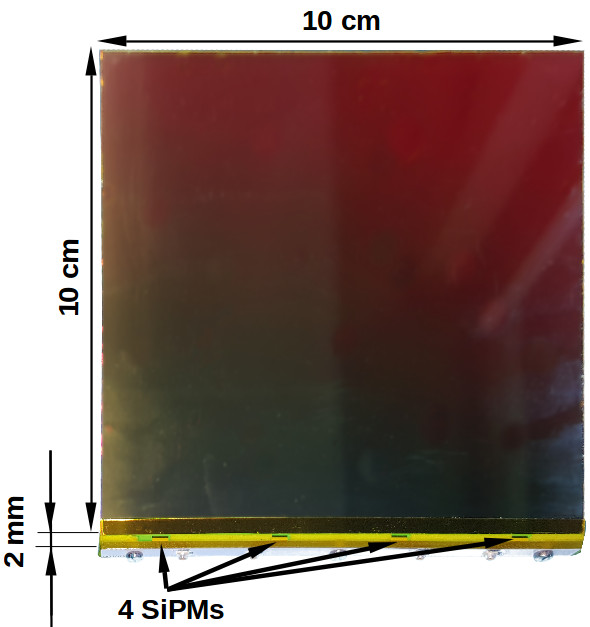
\includegraphics[width=.5\textwidth]{arclight/prototype}
	\caption[\SI{10 x 10}{\centi\metre} \glsentryshort{arclight} prototype]{%
		\SI{10 x 10}{\centi\metre} \acrshort{arclight} prototype.
		Four \acrshortpl{sipm} can be seen at the lower side, soldered to a narrow \acrshort{pcb} providing coaxial connectors for signal readout.
		The rest of the sensor area is dielectric.
	}
	\label{fig:arclight_prototype}
\end{figure}

Most of the following has been published in~\cite{arclight}.
The \AL{} is designed to minimise the occupied volume while maximising the area coverage of \glspl{sipm}.
This is achieved by coupling them to a passive light collector.
As mentioned above, principles based on full reflection on a polymer-\lar{} interface are not suitable.
Instead, \AL{} is based on the light trapping principle of the \gls{arapuca} sensor~\cite{arapuca}.
\gls{arapuca} works by trapping the photons inside a cavity made of walls covered by highly reflective materials.
One of the walls is formed of a dichroic film, a material transparent to certain wavelengths while highly reflective to others.
On the outside this film is coated with \gls{tpb}, which shifts the \lar{} scintillation light to the blue range, where the dichroic film is transparent.
The inner surface of the film is covered by a second \gls{wls}, shifting the light to green, which is reflected by the dichroic film and therefore trapped inside the cavity.
One or more \glspl{sipm} are mounted inside the cavity to collect the trapped photons.
\AL{} improves the \gls{arapuca} design by replacing the empty cavity with a solid transparent polymer sheet doped with a \gls{wls} dye.
This makes it substantially more robust and compact, especially when scaled up to larger areas.

\begin{figure}[tbp]
	\centering
	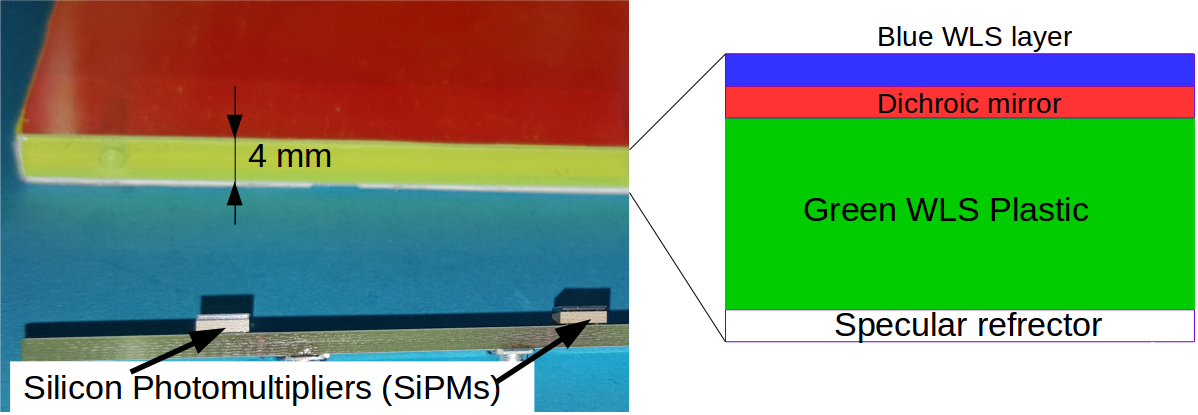
\includegraphics[width=\textwidth]{arclight/structure}
	\caption[\glsentryshort{arclight} light collector cross-section]{%
		\acrshort{arclight} light collector cross-section near a corner.
		The structure is mechanically supported by a \SI{4}{\milli\metre} thick \acrshort{wls} plastic.
		Its front is covered with a dichroic mirror film while the edges and the back face are covered with a dielectric specular reflector foil.
		The outer surface of the dichroic mirror is coated with \acrshort{tpb} to shift the \acrshort{lar} \acrshort{vuv} scintillation light to the blue range, where the dichroic film is transparent.
		At the bottom of the left picture two of the four \acrshortpl{sipm} mounted to the carrier \acrshort{pcb} are visible.
	}
	\label{fig:arclight_structure}
\end{figure}

A \SI{10 x 10}{\centi\metre} \AL{} prototype is shown in Figure~\ref{fig:arclight_prototype}.
The ratio of sensitive area to total area is \SI{98}{\percent} with the remaining \SI{2}{\percent} occupied by a \gls{pcb} carrying four \emph{Hamamatsu S13360-3050VE} \glspl{sipm}~\cite{arclight_sipm} with a sensitive area of \SI{3 x 3}{\milli\metre} each.
The inside of \AL{} is made of a \SI{4}{\milli\metre} thick \emph{Eljen Technology EJ-280} \gls{wls} plate~\cite{arclight_wls}.
Its sides are laminated with reflective films.
The back face and the edges are covered with a \emph{3M Vikuiti ESR} dielectric specular reflector foil~\cite{arclight_esr} having $\approx \SI{98}{\percent}$ reflectance in the visible light range.
A \emph{3M DF-PA Chill} dichroic mirror~\cite{arclight_dichroic} covers the front face.
It is transparent in the blue and has a high reflectance in the green spectral range.
Both films are held in place by thin layers of transparent adhesive.
To shift the \gls{vuv} scintillation light produced in \lar{} to the blue transparent range of the dichroic mirror its outer surface is coated with \gls{tpb}.
A cross-section of the structure of \AL{} is depicted in Figure~\ref{fig:arclight_structure}.

\begin{figure}[tbp]
	\centering
	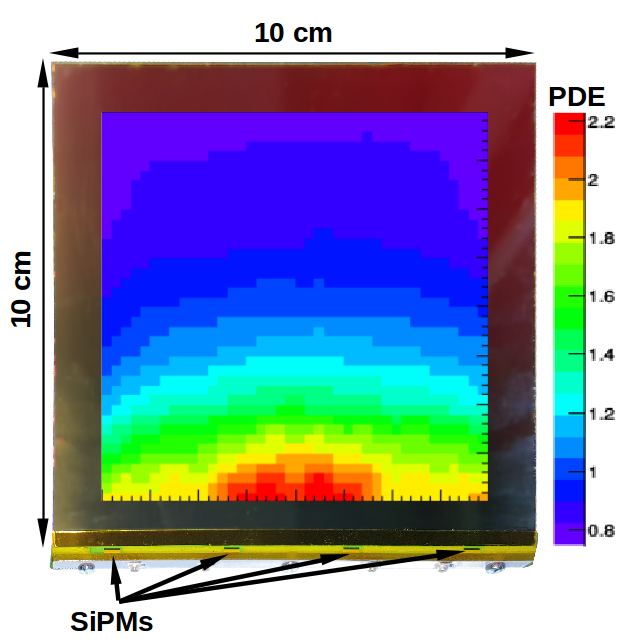
\includegraphics[width=\textwidth]{arclight/PDE}
	\caption[Measured \glsentryshort{arclight} \glsentryshort{pde}]{%
		Measured \acrshort{pde} for the \SI{10 x 10}{\centi\metre} \acrshort{arclight} prototype (background image), at room temperature.
		The \acrshort{pde} is given in \si{\percent}.
	}
	\label{fig:arclight_pde}
\end{figure}

The \gls{pde} was measured at room temperature using an \ce{^{241}Am} source, previously calibrated with a \gls{pmt}.
A \gls{pde} of \SIrange{0.8}{2.2}{\percent} was measured.
Figure~\ref{fig:arclight_pde} shows the \gls{pde} as a function of the position on the light collector, overlaid on a picture of the prototype for reference.
The increase in \gls{pde} near the \glspl{sipm} is likely caused by photons hitting the \glspl{sipm} directly with no prior reflection from the dichoic mirror.
Due to the angular dependence of the dichroic mirror's reflectance about \SI{30}{\percent} of the light is lost during the first reflection.
Once reflected, a photon is trapped inside \AL{} because of the specular nature of the reflection on all faces.
Additionally, the average \gls{pde} was calculated from theory to be \SI{0.7 +- 0.4}{\percent}, in agreement with the measurements.
More details on the calculations and the calibration of the measurement can be found in~\cite{arclight}.

\begin{figure}[tbp]
	\centering
	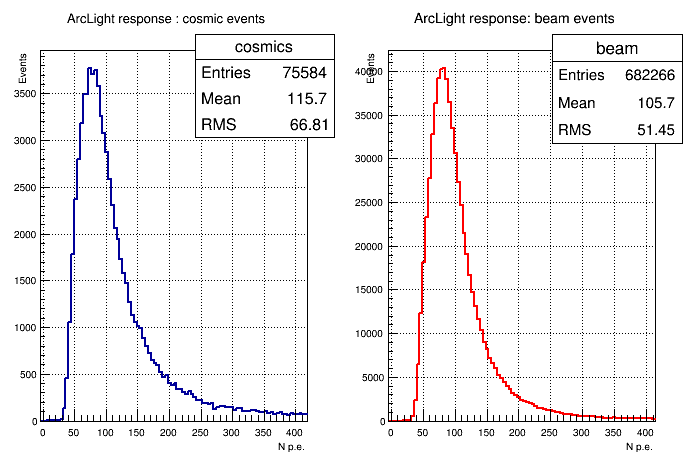
\includegraphics[width=\textwidth]{arclight/light_yield}
	\caption[\pixlar{} \glsentryshort{arclight} response]{%
		Distribution of observed number of photo-electrons (N p.e.)\ per event by the \acrshort{arclight} module in the \pixlar{} test beam demonstrator at \acrshort{fail}.
		The response is shown for cosmic (blue) and beam events (red).
	}
	\label{fig:arclight_pixlar_response}
\end{figure}

The measurements described above were performed at room temperature.
A \SI{43 x 15}{\centi\metre} \AL{} module was successfully operated at \lar{} temperatures in the \pixlar{} test beam demonstrator at \gls{fail}, described in Section~\ref{sec:ac_pixlar}.
Figure~\ref{fig:arclight_pixlar_response} shows the response for beam (red) and cosmic events (blue).
Cosmic events yield a mean of \num{115.7} photo-electrons while beam events produce slightly less light with a mean of \num{105.7} photo-electrons.
The time evolution of the mean photo-electron yield per event in beam (magenta) and cosmic ray (blue) mode is depicted in Figure~\ref{fig:arclight_pixlar_stability}.
Secondary beam energy and bending magnet current, selecting the momentum range of the tertiary beam, are also plotted for reference.
It can be seen that the photo-electron yield is approximately constant over several weeks.
The jumps in the response to beam events can be explained by the switching between different beam configurations.

\begin{figure}[tbp]
	\centering
	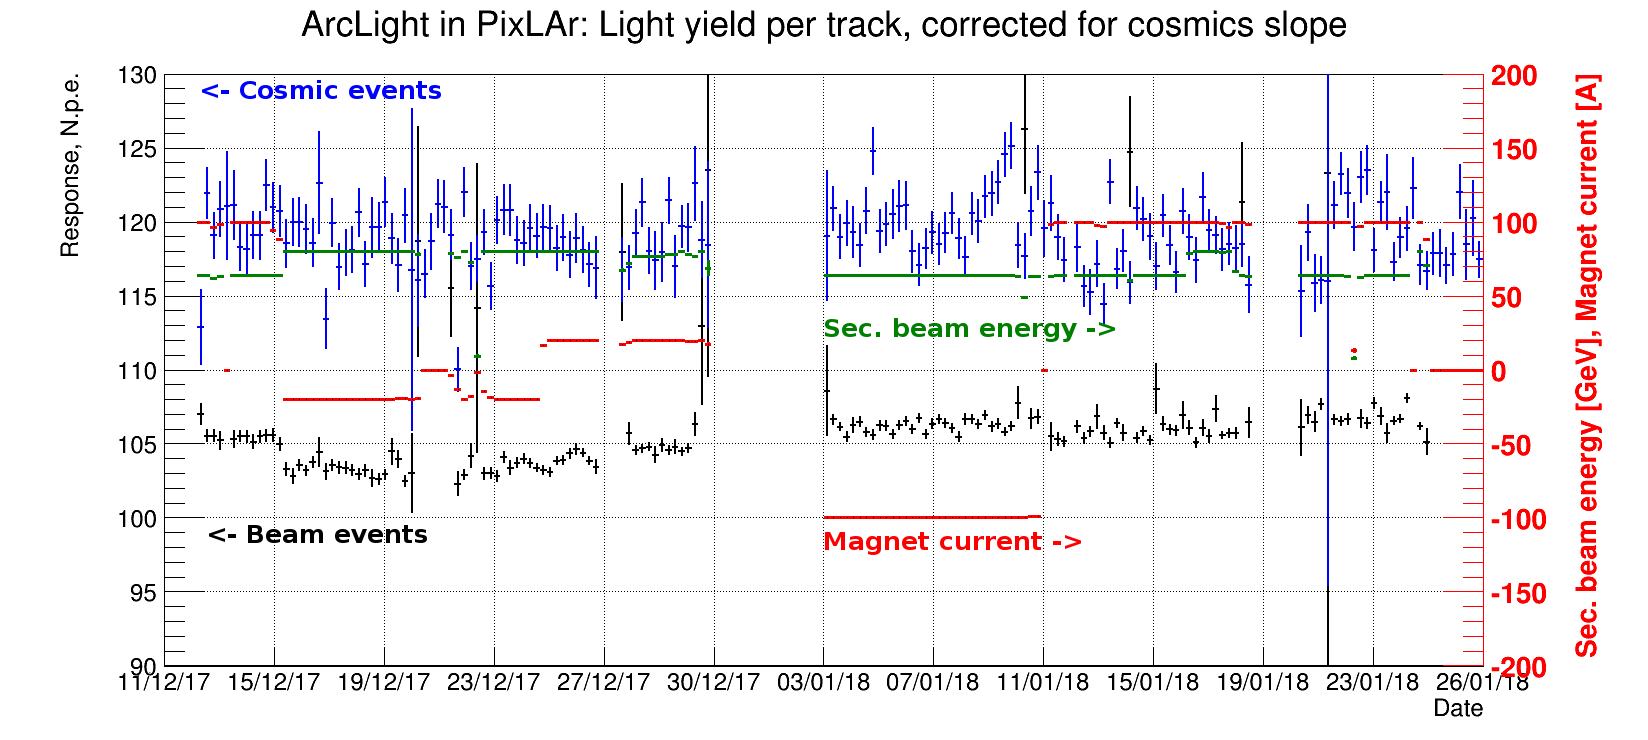
\includegraphics[viewport=0 0 1648 690, clip, width=\textwidth]{arclight/stability_cosm_beam_mod}
	\caption[\pixlar{} \glsentryshort{arclight} response stability]{%
		Mean observed number of photo-electrons (N p.e.)\ per event by the \acrshort{arclight} module in the \pixlar{} test beam demonstrator at \acrshort{fail}, over several weeks.
		The response is shown for cosmic (blue) and beam events (black).
		For reference the secondary beam energy (green) and the bending magnet current (red) are shown.
	}
	\label{fig:arclight_pixlar_stability}
\end{figure}


\section{Light Readout Summary}
\label{sec:studies_light-col-summary}

Classic \gls{pmt}-based light readout schemes for \lartpc{}s occupy large inactive volumes.
\glspl{sipm} are much smaller but so is their sensitive area.
I successfully used a cold \gls{sipm}-based light readout to trigger the charge readout of a pixelated \lartpc{} prototype.
\AL{} is a new light readout system based on the \gls{arapuca} light trap principle to increase the sensitive area of \glspl{sipm}.
Initial characterisations indicate a \gls{pde} of $\sim{\SI{1}{\percent}}$.
It can be installed inside the field cage of a \lartpc{} due to its low volume and the dielectric nature of the light collector.
	\chapter{A Novel Implementation of the \lartpc{} Technology}
\label{chap:ac}


\section{Results from the First Measurements with the \AC{} Pixel Demonstrator}
\label{sec:ac_viper}

This chapter describes the results obtained from the first pixelated \lartpc{} prototype for the \AC{} project (see Chapter~\ref{sec:ac_argoncube}).
While many of the individual systems, such as the high-voltage system, light and charge readout, have been described in previous chapters, a short overview of the implementation is given here.


\subsection{Pixel PCB Design}
\label{sec:ac_viper_pcb}
 
The pixelated anode plane, shown in Figure~\ref{fig:viper_pixies}, was produced as a conventional Printed Circuit Board (PCB). 
The pixelated area is \SI{100}{\milli\metre} across, the pixels are formed of \SI{900}{\micro\metre} vias with a pitch of \SI{2.54}{\milli\metre}.
An inductive focusing grid surrounds the pixels, it is made from \SI{152.4}{\micro\metre} copper traces split into 28 regions.
There are \num{6 x 6} pixels per region, giving a total of 1008 pixels. 

\begin{figure}[htb]
	\centering
	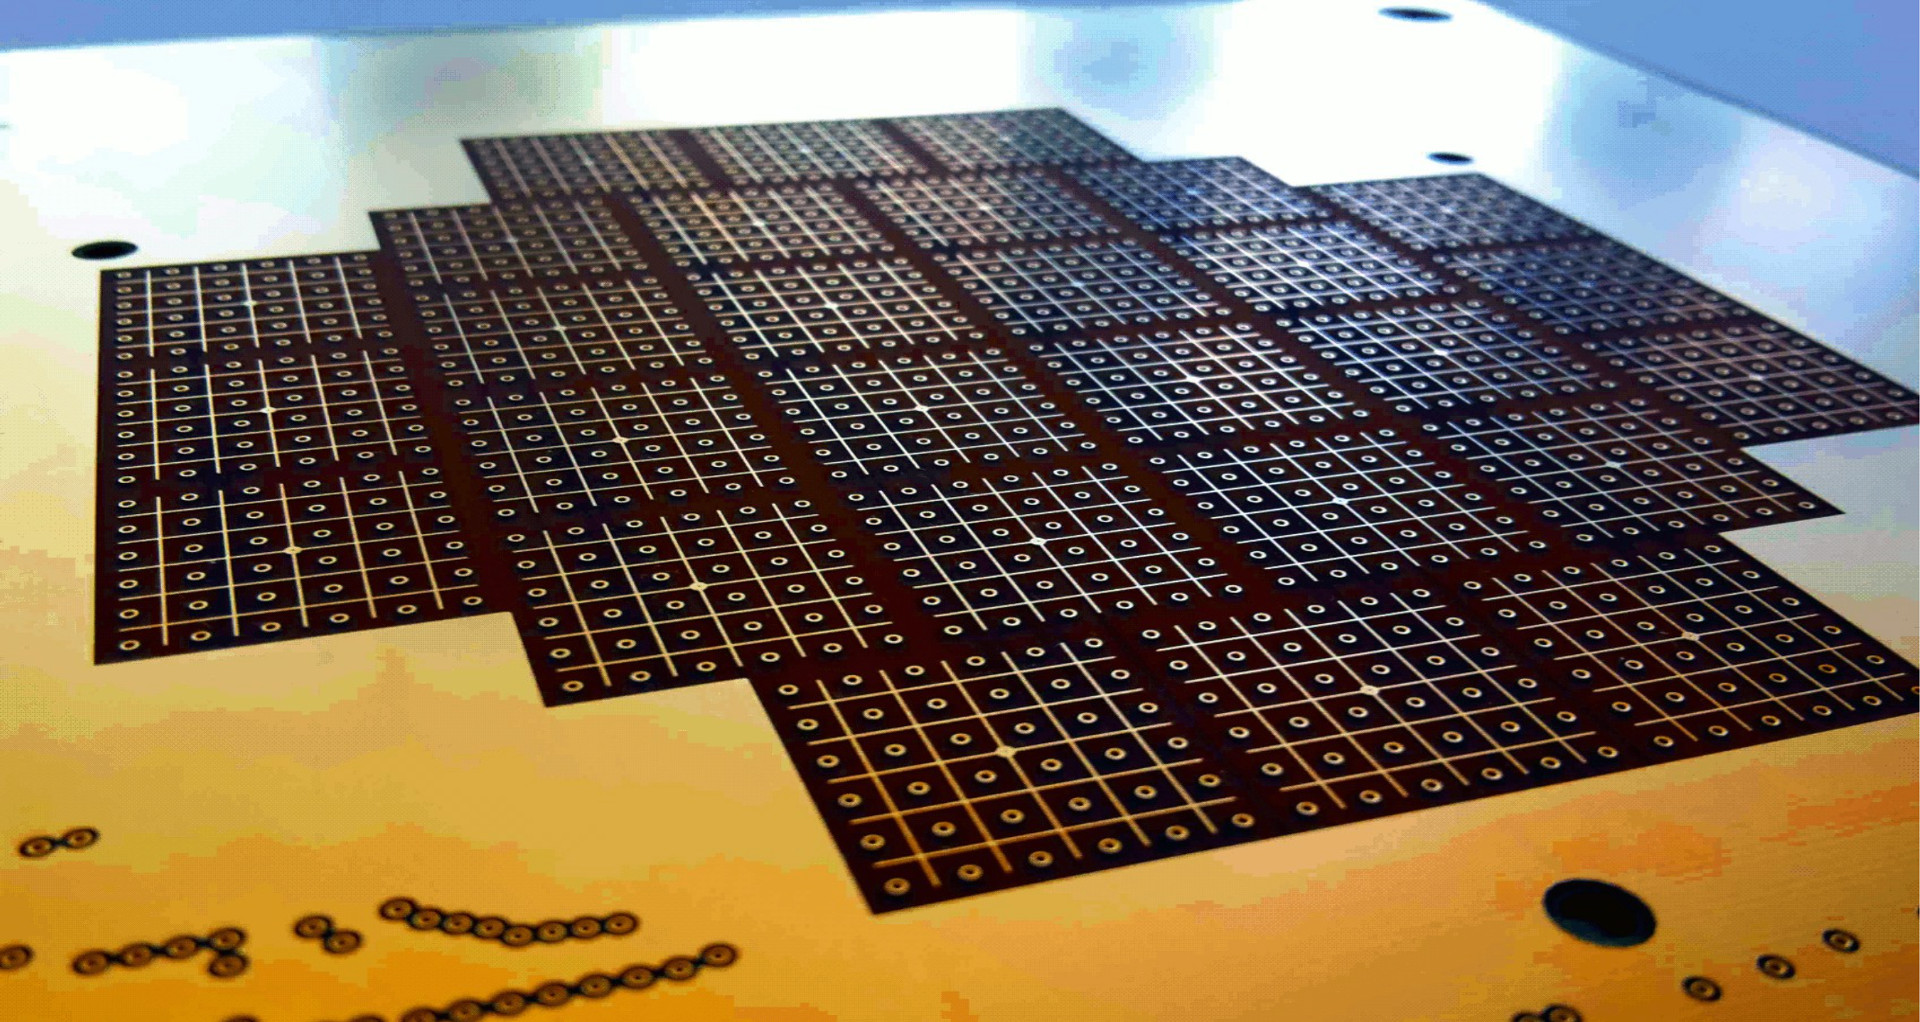
\includegraphics[width=0.65\linewidth]{viper/pixies}
	\caption{Initial (July 2016) pixelated anode PCB. The pixelated readout area is \SI{100}{\milli\metre} in diameter.
	Each charge collection pixel is a \SI{900}{\micro\metre}, at a pitch of \SI{2.54}{\milli\metre}, inductive focusing grids formed of \SI{152.4}{\micro\metre} copper traces surround the pixels.
	There are 28 inductive focusing grids with 36 pixels per region, a total of 1008 pixels.}
	\label{fig:viper_pixies}
\end{figure}

Vias were used for pixels instead of pads in order to minimise capacitance.
As detailed in Section~\ref{sec:studies_electronics}, it is important that capacitance is minimised when amplifying charge.
To further minimise parasitic capacitance, the PCB design was optimised by removing unnecessary ground planes, routing signal tracks outside necessary ground planes, and increasing the thickness of the PCB to \SI{3.5}{\milli\metre} from an initial \SI{1.75}{\milli\metre}. 
The resulting capacitance at each pixel is $\order{\SI{50}{\pico\farad}}$.

The pixels are directly connected to the preamplifiers while the inductive focusing grids are decoupled via \SI{10}{\nano\farad} capacitors.
Additionally, the bias voltage is filtered at the input by another \SI{10}{\nano\farad} and \SI{10}{\mega\ohm}.
The full schematic of the bias circuit is depicted in Figure~\ref{fig:viper_pcb_schematic}.

\begin{figure}[htb]
	\centering
	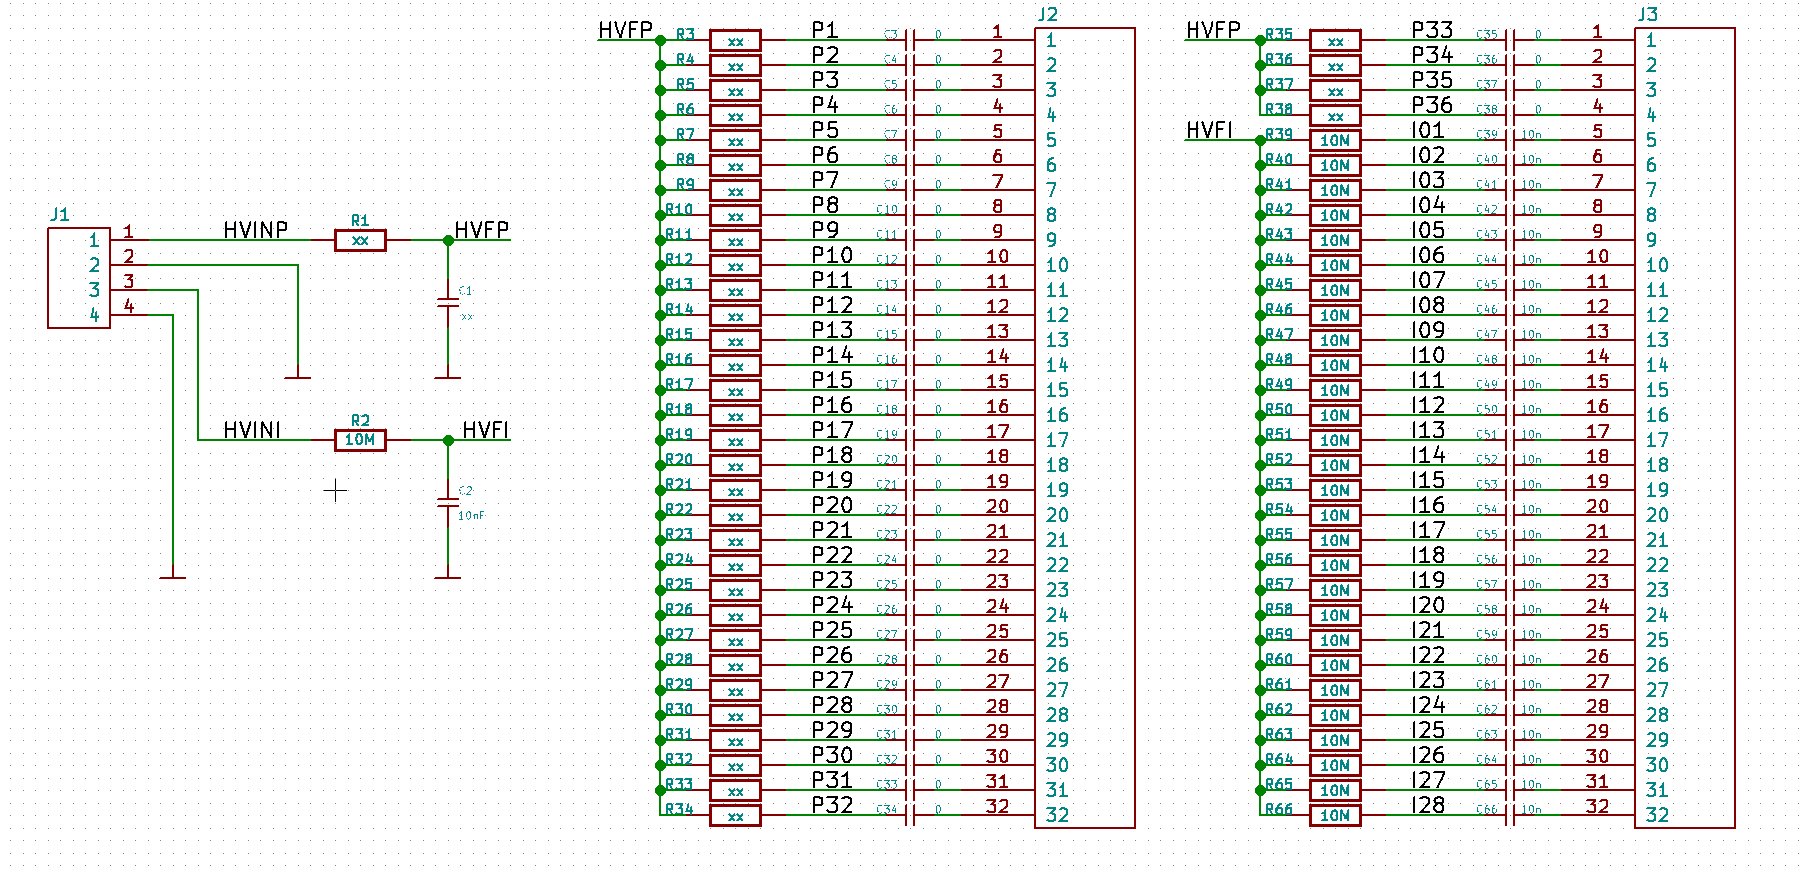
\includegraphics[width=\textwidth]{viper/pixel_pcb_schematic}
	\caption{Schematic of the bias circuit for the \AC{} pixel demonstrator PCB.
	On the left, the pinheader connected to the bias HV power suplly is shown. In the middle and on the right are the connections to the pixels and inductive ROI grids.
	The connections to the preamplifier inputs are located at the positions of numbers P1--P36 (pixels) and I1--I28 (ROIs).
	For simplicity and universality, the same circuit was used for both pixels and ROIs eventhough for the measurements described in this work, only the inductive ROI grids were biased.
	Therefore, the ROIs are connected as depicted (R2 and R39--R66, C2 and C39--C66).
	As the pixels need not be biased, they are directly connected to the preamplifiers by leaving R3--R38 unpopulated and replacing C3--C38 by \SI{0}{\ohm} resistors.
	Additionally, R1 is \SI{0}{\ohm} and C1 unpopulated, and by connecting pin 1 of J1 to ground, all unused PCB traces are grounded.}
	\label{fig:viper_pcb_schematic}
\end{figure}

The bias on the inductive focusing grids had to be sufficient to allow full charge transparency (all charge collected by the pixels), yet low enough to minimise any risk of damaging the cold coupling capacitors.
It was increased incrementally until transparency was observed at \SI{300}{\volt}. 
Simulation suggest this was only \SI{95}{\percent} transparency, with \SI{100}{\percent} at \SI{350}{\volt} (see Figure~\ref{fig:viper_transparency}).
The simulation available at the time of the measurement contained a bug resulting in an underestimation of the bias voltage required for full transparency.
During measurments, the bug became apparent and full transparency had to be estimated by looking at live data from the detector.
Due to the limited accuracy of this method, measurements were not taken up to the bias voltage for full transparency suggested by the (corrected) simulation.~\cite{francypants}

\begin{figure}[htb]
	\centering
	\includegraphics[width=\textwidth]{viper/transparency}
	\caption{Measured and simulated transparency versus bias voltage of the \AC{} pixel demonstrator.
	The simulation available at the time of the measurement contained a bug resulting in an underestimation of the bias voltage required for full transparency.
	During measurments, the bug became apparent and full transparency had to be estimated by looking at live data from the detector.
	Due to the limited accuracy of this method, measurements were not taken up to the bias voltage for full transparency suggested by the (corrected) simulation.~\cite{francypants}}
	\label{fig:viper_transparency}
\end{figure}

\afterpage{\clearpage}


\subsection{TPC}
\label{sec:ac_viper_tpc}

The pixel demonstration TPC, shown in Figures~\ref{fig:viper_cad}~and~\ref{fig:viper_v1per}, is cylindrical with an inner diameter of \SI{101}{\milli\metre} and a \SI{590}{\milli\metre} drift length. 
The TPC operated with a drift field of \SI{1}{\kilo\volt\per\centi\metre}, corresponding to a total drift time of \SI{281}{\micro\second} at \SI{2.1}{\milli\metre\per\micro\second}.~\cite{protoLASER}

\begin{figure}[htb]
	\centering
	\includegraphics[width=0.9\linewidth]{viper/tpc_cad}
	\caption{\small Engineering drawing of the pixel demonstration TPC; \SI{590}{\milli\metre} drift length; \SI{6.25}{\milli\metre} field cage spacing; \SI{101}{\milli\metre} internal diameter.}
	\label{fig:viper_cad}
\end{figure}
 
The field-cage consists of aluminium rings supported by clear acrylic rings, with a cathode formed of a brass disc. 
The dimensions of the field-cage and cathode are shown in Figure~\ref{fig:viper_cad}.
Alternating acrylic rings are split, to allow for the circulation of purified \lar{} within the TPC volume.
Four square section PolyAmide-Imide (PAI) uprights support the cathode and field cage, with PolyEther Ether Ketone (PEEK) screws fixing the pillars to the acrylic rings.
The four PAI uprights connect to a PAI frame which supports the anode plane and the light readout Silicon PhotoMultipliers (SiPMs), see Figure~\ref{fig:viper_v1per}.   

The resistive divider consists of a chain of \SI{100}{\mega\ohm} Vishay Rox metal oxide resistors (ROX100100MFKEL).
Each resistor is soldered to its neighbour, and fixed to the field cage at each joint with an M3 screw.   

\begin{figure}[htb]
	\centering
	\includegraphics[width=0.26\linewidth]{viper/viper_original}
	\includegraphics[width=0.62\linewidth]{viper/viper_sipm}
	\caption{\small  Left: Photograph of the  pixel demonstration TPC at Bern, with the HV feedthrough.
	Right: Close-up of the light collection system, showing wavelength shifting fibres coupling SiPMs to the TPB-coated light guides.}
	\label{fig:viper_v1per}
\end{figure}

The acrylic rings provide the light collection; their inner surfaces are machine-polished and coated with the WaveLength Shifter (WLS) TetraPhenylButadiene (TPB). 
The coating method is based on~\cite{TPBcoating}.
\SI{0.5}{\gram} of TPB and \SI{0.5}{\gram} of acrylic flakes were dissolved in \SI{50}{\milli\liter} of toluene and then mixed with \SI{12}{\milli\liter} of ethanol, which serves to increase the coating homogeneity. 
Three layers of the coating were applied by hand, with a fine brush. 

\SI{1}{\milli\metre} diameter WLS fibres (Kuraray Y11(200)M) couple the acrylic rings to the four Hamamatsu S12825-050P SiPMs mounted close to the anode, see Figure~\ref{fig:viper_v1per}. 
The SiPMs and their front-end electronics were adapted from those developed at Bern for the cosmic ray taggers used in \uboone{} and \sbnd{}~\cite{crt, crt_feb}.
For operation in \lar{}, the SiPM bias voltages had to be reduce from $\approx$~\SI{70}{\volt} to \SI{53}{\volt}, in order to limit the gain.   
In the front-end electronics, two coincidences of two out of the four SiPMs are formed and combined by means of a logic \textit{OR} operation. 
This coincidence is used in order to improve trigger purity.

\afterpage{\clearpage}


\subsection{Ancillary Infrastructure}
\label{sec:ac_viper_infrastructure}

The pixel demonstration TPC is housed in a double-bath vacuum-insulated cryostat with the outer bath open to atmosphere.
A diameter of \SI{50}{\centi\metre} and a height of \SI{110}{\centi\metre} give an inner volume of $\approx \SI{200}{\litre}$ of liquid argon.
This is the same cryostat that was used for the HV studies described in Section~\ref{sec:studies_hv}.
The \lar{} filtering method is the same as described in~\cite{2photonAbs}, with \lar{} filtered first on filling through a pair of Oxysorb-Hydrosorb filters, and then recirculated through a single custom-made filter containing both activated copper and silica gel.
\lar{} purity is estimated to be in accordance with~\cite{2photonAbs}, with impurity concentrations $\order{\SI{1}{ppb}}$ of oxygen-equivalent, which corresponds to a charge lifetime of \SI{290+-30}{\micro\second}.

The HV feedthrough remains unchanged from the breakdown studies (Section~\ref{sec:studies_hv}); a PET-C polymer dielectric capable of potentials as high as \SI{-130}{\kilo\volt}.
A low-pass filter was added between the power supply and feedthrough, which consists of an \SI{800}{\pico\farad} decoupling capacitor grounded between two \SI{100}{\mega\ohm} resistors connected in series, i.e.\ an RC low-pass filter with an additional protection resistor at the output.
For proper insulation, the whole assembly is submerged in transformer oil.

\afterpage{\clearpage}


\subsection{Signal to noise ratio}
\label{sec:ac_viper_snr}

To assess the Signal to Noise Ratio (SNR), dedicated noise data was taken employing a \SI{5}{\hertz} random trigger.
The data of \num{5000} events was combined.
Subsequently, all pixel and ROI channels were combined separately and filled into respective amplitude distribution histograms.
Finally, the standard deviation of the noise was calculated by fitting a Gaussian to the amplitude distribution.
This value was used to calculate the noise for pixel and ROI channels according to
\begin{IEEEeqnarray}{rCl}
	\m{SNR} & = & \frac{S}{\sigma} \qc
	\label{eq:viper_snr}
\end{IEEEeqnarray}
where $S$ is the signal and $\sigma$ is the noise standard deviation from the Gaussian fit.
As can be seen in the left plot in Figure~\ref{fig:viper_unfilteredRawData}, one of the pixel channels is significantly noisier in comparison to others, likely caused by a broken preamplifier.
Therefore, this channel was blinded for the SNR calculations.
The resulting equivalent noise charge is \SI{1095}{\elementarycharge} for the pixel channels and \SI{982}{\elementarycharge} for the inductive ROI channels

The signal $S$ is often taken for a Minimum-Ionising Particle (MIP) as this is at the lower end of the signal range interesting for neutrino physics.
Getting a clean MIP sample from experimental data requires a calibrated reconstruction which was not available at the time of writing.
Therefore, the MIP signal was estimated from theory assuming an energy loss of \SI{2.1}{\mega\electronvolt\per\centi\metre} (see Section~\ref{sec:nu-detection_fs}).
This can be converted to charge loss using the energy required to produce one electron-ion pair from Table~\ref{tab:lartpc_larprop}: $W_{\m{i}} = \SI{23.6}{\electronvolt\per\elementarycharge}$.
Additionally, charge recombination, diffusion and lifetime need to be taken into account (see Section~\ref{sec:lartpc_lar}).
The recombination factor was measured by \icarus{}~\cite{icarusReco} and \argoneut{}~\cite{argoneutReco} and found to be $R_{\m{c}} \approx 0.7$ for a drift field of $\SI{1}{\kilo\volt\per\centi\meter}$.
With \AT{}~\cite{AT}, Bern measured a transverse diffusion coefficient $D_{\m{T}} = \SI{5.3}{\centi\metre\squared\per\second}$ at \SI{0.25}{\kilo\volt\per\centi\metre} while Gushchin et al.~\cite{gushchin} report a value of $D_{\m{T}} = \SI{13}{\centi\metre\squared\per\second}$ at \SI{1}{\kilo\volt\per\centi\metre}.
Even using the more conservative value, this results in a transverse spread of $\approx \SI{0.9}{\milli\metre}$ for the pixel demonstrator drift time of $t = \SI{281}{\micro\second}$, according to Equation~\eqref{eq:lartpc_lar-diff}.
This value lies well below the pixel pitch of $d_{\m{p}} = \SI{2.54}{\milli\metre}$.
Considering that the longitudinal component is smaller than the transverse ~\cite{lngDet}, diffusion is neglected completely for these calculations.
Finally, the lifetime of \SI{290}{\micro\second} will result in the reduction of charge by a factor of $\approx\num{0.38}$ over the full drift distance (Equation~\eqref{eq:lartpc_lar-lifetime}).
Combining this, the signal is 
\begin{IEEEeqnarray}{rCl}
	S & = & \dv{E}{x}_{\m{MIP}} \frac{R_{\m{c}} d_{\m{p}}}{W_{\m{i}}} = \SI{15821}{\elementarycharge} \qc
\end{IEEEeqnarray}
for a charge deposited adjacent to the readout plane, and $S = \SI{6004}{\elementarycharge}$ for a charge deposited adjacent to the cathode.

Table~\ref{tab:viper_snr} lists the SNR values obtained from these signal values and the aforementioned measured equivalent noise charge, using Equation~\eqref{eq:viper_snr}.

\begin{table}[htb]
	\centering
	\caption{SNR values obtained from Equation~\eqref{eq:viper_snr} using the theoretical signal of a MIP at the readout plane or cathode, respectively combined with the average equivalent noise charge for pixel and ROI channels obtained from measurements.}
	\label{tab:viper_snr}
	\begin{tabu} to \textwidth {llS}
		\toprule
		Channel &	MIP at &		{SNR} \\
		\midrule
		Pixel &		Readout plane &	14 \\
		Pixel &		Cathode &		5.5 \\
		ROI &		Readout plane &	16 \\
		ROI &		Cathode &		6.1 \\
		\bottomrule
	\end{tabu}
\end{table}

\afterpage{\clearpage}


\subsection{3D track reconstruction}
\label{sec:ac_viper_3d}

To demonstrate 3D track reconstruction, several thousand cosmic ray events were collected, many of which are MIPs, mostly muons.
The charge readout was triggered by the light readout described above.

The reconstruction procedure comprises five steps: noise filtering, hit finding, hit matching, ambiguity rejection, and track fitting.
These steps are explained in the following and depicted in Figures~\ref{fig:viper_unfilteredRawData} through~\ref{fig:viper_kalman}, all taken from the same MIP (cosmic muon) event.

In the first step, a noise-filtering algorithm is applied to the raw data.
As can be seen from Figure~\ref{fig:viper_unfilteredRawData}, the noise is largely correlated across all the channels.
\footnote{Due to the much higher signal levels, the noise is barely visible on the pixel channels on the left.}
This common-mode correlation can be exploited by the noise filter algorithm.
The following is done separately for the all pixel and ROI channels of each event.
Similarly to the SNR calculation, all samples are filled into an amplitude distribution histogram for each channel, and subsequently fitted with a Gaussian.
A noise band is defined per channel with its centre equal to the mean of the Gaussian and its width equal to the standard deviation multiplied by a tunable scaling factor.
The amplitudes of all channels within the corresponding noise band are then averaged for each sample.
Finally, this average is subtracted from each channel at the corresponding sample.
This technique was chosen because it effectively suppresses the dominating common mode noise.
At the same time, spurious signals produced by high amplitudes from collected charge distorting the average are kept to a minimum by only accepting values within the noise band.
The effectiveness of the filtering can be seen in Figure~\ref{fig:viper_filteredRawData}, which shows the same data as Figure~\ref{fig:viper_unfilteredRawData} post filtering.

\begin{figure}[htb]
	\centering
	\includegraphics[width=\textwidth]{viper/event967_rawUnfilteredPixel}\\
	\includegraphics[width=\textwidth]{viper/event967_rawUnfilteredROI}
	\caption{Unfiltered raw data of a typical MIP event (the same event as in Figures~\ref{fig:viper_unfilteredRawData}~through~\ref{fig:viper_kalman}). The top plot shows pixel data while the bottom plot shows ROI data.}
	\label{fig:viper_unfilteredRawData}
\end{figure}

\begin{figure}[htb]
	\centering
	\includegraphics[width=\textwidth]{viper/event967_rawFilteredPixel}\\
	\includegraphics[width=\textwidth]{viper/event967_rawFilteredROI}
	\caption{Filtered data of a typical MIP event (the same event as in Figures~\ref{fig:viper_unfilteredRawData}~through~\ref{fig:viper_kalman}).
	The top plot shows pixel data while the bottom plot shows ROI data}
	\label{fig:viper_filteredRawData}
\end{figure}

The second step applies a recursive pulse finding algorithm.
The following is performed for each channel independently.
Most thresholds employed by the pulse finder are, again, defined in terms of noise amplitude.
Therefore, noise mean and standard deviation are recalculated after noise filtering.
A peak threshold is defined by multiplying the noise standard deviation by a variable scaling factor and adding the noise mean.
Then, the sample with the highest amplitude is found.
If it is below threshold, the process stops and proceeds to the next channel.
Otherwise, the pulse is scanned in positive and negative directions until it crosses respective lower noise thresholds.
After this, the whole pulse is deleted from the data and the process starts over with finding the new maximum sample and checking it against the peak threshold.
For stability reasons, the peak threshold relative to noise levels is compared against an absolute threshold and the higher of the two is applied.
The search is extended to the negative pulse for the bipolar ROI pulses.
The different thresholds employed and samples found by this process are illustrated in Figure~\ref{fig:viper_hitFinder}.

\begin{figure}[htb]
	\centering
	\includegraphics[width=\textwidth, page=1]{viper/event967_pixel2_hit8}\\
	\includegraphics[width=\textwidth, page=3]{viper/event967_pixel2_hit8}
	\caption{Pulse shapes of a single pixel (top) and ROI (bottom) hit of a typical MIP event (the same event as in Figures~\ref{fig:viper_unfilteredRawData}~through~\ref{fig:viper_kalman}).
	Superimposed are the thresholds of the hit finder algorithm. Horizontal lines represent thresholds: the solid is the minimum threshold required to be crossed for a pulse to be detected, and dashed are the thresholds used to detect the pulse edges.
	Vertical lines represent the corresponding detected peak/edge samples.
	Colour indicates a positive (green) or negative (red) pulse, or a zero crossing (yellow).}
	\label{fig:viper_hitFinder}
\end{figure}

Identified pulses are then combined into 3D hits by matching pixels pulses to ROI pulses.
For this proof of concept, this is done rather primitively by matching any pulses coinciding in time.
In Figure~\ref{fig:viper_hitFinder}, a pixel and ROI pulse are matched if their time slices, defined by the vertical dashed lines, overlap.
This third step results in a rather high amount of ambiguities but assures that no hits are missed.

To resolve the ambiguities, a Principal Component Analysis (PCA) is applied to the 3D space points in a fourth step.
This technique is well established and described in literature, e.g.~\cite{pca}.
Therefore, it shall be explained here only briefly.
The basic idea is to calculate three orthogonal eigenvectors of the 3D space point cloud.
A graphic interpretation of these eigenvectors are the three axis of an ellipsoid fitted to the data points.
In case the points form a track, one of these eigenvectors will have a much higher eigenvalue than the other two.
This eigenvector is taken as an estimate for the track direction.
The ambiguities can be resolved by selecting the one closest to the track estimate.
Furthermore, this procedure can be used to recursively reject outliers by forming a cylinder around the track estimate with a radius proportional to the second largest eigenvalue.
All hits outside this cylinder are rejected.
The procedure can be repeated by rerunning the PCA on the remaining points and performing another outlier rejection.
In a later stage of reconstructing more complex events, this algorithm can potentially be used to cluster 3D space points in order to separate multiple tracks.
The PCA ambiguity rejection is illustrated in Figure~\ref{fig:viper_pca}.

\begin{figure}[htb]
	\centering
	\includegraphics[viewport=600 0 1000 2000, clip, height=\textwidth, angle=90]{viper/event967_pulses_q} \\
	\includegraphics[viewport=600 0 1000 2000, clip, height=\textwidth, angle=90]{viper/event967_pulses_a_pca} \\
	\includegraphics[viewport=600 0 1000 2000, clip, height=\textwidth, angle=90]{viper/event967_pulses_a_det}
	\caption{Reconstructed 3D hits from the hit finder.
		The passing particle is most likely a cosmic \Pgm entering from the left (the same event as in Figures~\ref{fig:viper_unfilteredRawData}~through~\ref{fig:viper_kalman}).
		Drift direction is from right to left.
		Pulse shape is encoded as thickness.
		In the top plot, colour codes the amount of collected charge.
		The middle plot illustrates the ambiguity resolution employing a principal component analysis.
		Green hits are accepted while dark red ones are rejected.
		This is achieved by selecting the ambiguity closest to the eigenvector of the point cloud with the largest eigenvalue, represented by the blue line.
		In the bottom plot, the degree of ambiguity is colour-coded: Light green are unambiguous hits while dark green are selected solutions of ambiguous hits.
		Dark red through black are rejected solutions of ambiguous hits where darker colour represents a higher degree of ambiguity.
		As this is a quite clean track with only few short $\delta$ rays, there are no outliers rejected other than the multiplexing ambiguities.}
	\label{fig:viper_pca}
\end{figure}

The final step consists of a Kalman filter.
For this, the well-established GENFIT track fitting package~\cite{genfit1, genfit2} was used.
Ionisation losses and multiple scattering are taken into account.
The particle is assumed to be a minimum-ionising muon with an initial momentum of \SI{260}{\mega\electronvolt\per\clight} in the direction of the track estimate from the PCA.
A recursive algorithm capable of dealing with outliers was chosen, a so-called \emph{deterministic annealing filter}.
This works by assigning successively lower weights to outliers with each recursion step.
For more details, see the respective publications~\cite{genfit1, genfit2}.
The resulting track is shown in Figure~\ref{fig:viper_kalman}.

\begin{figure}[htb]
	\centering
	\includegraphics[width=\textwidth]{viper/event967_kalman}
	\caption{Track fitted by the Kalman filter.
	The TPC volume is shown in faint grey.
	The passing particle is most likely a cosmic \Pgm entering from the left (the same event as in Figures~\ref{fig:viper_unfilteredRawData}~through~\ref{fig:viper_kalman}).
	Drift direction is from right to left.
	The yellow points are the input to the Kalman filter, the accepted hits from the principal components analysis.
	Blue is the output, a fitted track taking into account ionisation losses and multiple scattering in \lar{}.}
	\label{fig:viper_kalman}
\end{figure}

Technically, the Kalman filter would be capable of fitting the particle momentum or even particle type to the data.
At the time of this writing, this is not implemented yet.
In particular, the momentum stays roughly at the initial guess of \SI{260}{\mega\electronvolt\per\clight}, assuming a minimum ionising muon in liquid argon.
A potential explanation for this is that the resolution of the detector is too low to estimate momentum from multiple scattering.
Another explanation might be the hit finder missing hits due to non-optimal tuning.
Proper tuning of the reconstruction requires a full simulation chain of the detector which is not yet available.
Using data to tune the reconstruction is prone to the introduction of circular biases.
On the other hand, most of the difficulties emerge from the multiplexing ambiguities and their resolution.
While the presented almost full 3D readout has already reduced the reconstruction complexity compared to a classical wire readout, an ambiguity-free readout will make reconstruction another big step easier by completely eliminating the need to resolve ambiguities.

\afterpage{\clearpage}


\section{\pixlar{}}
\label{sec:ac_pixlar}

\begin{figure}[htb]
	\centering
	\includegraphics[width=\textwidth]{pixlar/pixlar_arclight}
	\caption{One of the two \pixlar{} readout half planes with the \AL{} module attached.}
	\label{fig:pixlar_arclight}
\end{figure}

After the successful test with cosmic muons at Bern, a bigger prototype of the pixel readout, employing the same multiplexing scheme, was built for a beam exposure in the \lariat{} experiment~\cite{lariat} at FNAL.
\lariat{} consists of the former \argoneut{}~\cite{argoneut} cryostat and \lartpc{} put into a test beam.
The tertiary beam line produces mainly pions and protons as well as electrons, muons and kaons at a lower rate.
Their momentum spectrum can be tuned from \SIrange{0.2}{2.0}{\giga\electronvolt\per\clight}.
\SI{550}{\litre} of \lar{} are contained in a cylindrical cryostat.
It houses a TPC with \SI{47}{\centi\metre} drift length and a \SI{40 x 90}{\centi\metre} readout plane parallel to the beam direction, resulting in an active volume of \SI{170}{\litre}.
For the pixel test, called \pixlar{}, the original wire planes were replaced by a \num{120 x 240} pixel readout.
At \SI{3}{\milli\metre} pitch, this gives an instrumented area of \SI{36 x 72}{\centi\metre}.
Due to constraints from the PCB manufacturer, the readout plane had to be split into two mirror-symmetric, electrically independent half planes.
Each \num{120 x 120} pixel half plane is divided into \num{8 x 15} ROIs of \num{15 x 8} pixels each.
The ROIs are oriented with their longer dimension parallel to the beam direction to reduce the multiplexing ambiguities.
One of the noise mitigation measures implemented for the Bern pixel demonstrator was to use the same differential warm signal path as used by \lariat{}.
Therefore, the charge readout electronics used in \pixlar{} are quite similar to the \AT{} chain described in Section~\ref{sec:studies_electronics_at} after the upgrades.
To trigger on scintillation light, one end of the TPC is equipped with a \SI{43 x 15}{\centi\metre} \AL{} module (see Section~\ref{sec:studies_light-col_al}), while the other end features an ARAPUCA~\cite{arapuca} detector for comparison.
Figure~\ref{fig:pixlar_arclight} shows one of the readout half planes with the \AL{} module attached.

\begin{figure}[htb]
	\centering
	\includegraphics[width=.445\textwidth]{pixlar/pixlar_event_side}
	\includegraphics[width=.545\textwidth]{pixlar/pixlar_event_top}
	\caption{\pixlar{} beam event.}
	\label{fig:pixlar_event}
\end{figure}

Over several weeks, beam and cosmic muon data was taken.
At the time of this writing, no official results were available.
Nevertheless, preliminary analyses indicate a successful scale-up of the pixelated \lartpc{} concept.
The achieved SNR seems to be comparable to what was reached with the prototype in Bern described above.
A recorded beam event is depicted in Figure~\ref{fig:pixlar_event}.

\afterpage{\clearpage}
	\section{The \AC{} Approach}
\label{sec:ac_argoncube}

To address the challenges mentioned in Section~\ref{sec:lartpc_challenges}, the \gls{help} group has formed the \AC{} collaboration, with the goal of developing a new fully-modular type of \lartpc{}.
Modularity reduces pile-up and allows for shorter drift-times, thus slackens the requirements on argon purity and \gls{hv}.
A modular detector also contains light within each module, allowing for a more accurate trigger system.
Maintenance and upgrading of a modular detector is much easier than for a monolothic one.


\subsection{Modularity}
\label{sec:ac_argoncube_mod}

\AC{} is made of self-contained \gls{tpc} modules sharing a common cryostat.
In case of a fault condition the affected module(s) can be shut down and repaired or replaced individually without affecting the rest of the detector.
During construction, one can start data taking as soon as the first module is operational and needs not wait for the commissioning of the whole detector.
A modular detector furthermore reduces event pile-up because the acquisition time is reduced to the size of one half module.
This is crucial in the high-multiplicity environments of future \lar{} neutrino detectors.
Finally, also trigger purity profits from a modular approach because scintillation light is contained within each module, allowing for a localised trigger.

\begin{figure}[htb]
	\centering
	\includegraphics[width=\textwidth, angle=-90]{ac/2x2/Normal-Module-4K}
	\caption[\AC{} module schematic]{%
		Engineering drawing of an \AC{} module.
	}
	\label{fig:ac_module}
\end{figure}

A module is made of a rectangular box with a square footprint and the height required by physics goals and/or sensitivity constraints.
The top and bottom flanges are made of stainless steel while the side walls are made from \SI{1}{\centi\metre} G10 sheets.
G10 is a glass-reinforced epoxy composite formerly used for \glspl{pcb}.
Its low density makes it more transparent for passing particles allowing for a performance comparable to a monolithic detector.
At the same time, the dead volume is drastically reduced compared to a monolithic design due to the comparably low cathode voltage (see Section~\ref{sec:dune-nd_ac}).
The modules are placed side-by-side in a bath of \lar{} where they can be extracted and reinserted as needed.
Pressure inside the modules is kept close to the bath pressure putting almost no hydrostatic force on the module walls.
Purity of the \lar{} is maintained within each module by means of a recirculation system (see Section~\ref{sec:ac_argoncube_cryo}).
As a result, the argon surrounding the modules needs not meet as stringent purity requirements as the argon inside.
Under normal operation conditions, all modules are inserted with only clearance distances between modules, and their top flanges sealed using indium.
The schematic of an \AC{} module is shown in Figure~\ref{fig:ac_module}.

To extract a module, the indium seal around the flange in question is removed.
The module is then slowly lifted up by a crane and the \lar{} is drained to the surrounding bath through a hydrostatic outlet valve at the bottom of the module by means of gravity.
On the bottom of the module, a blind flange is located with equal dimensions as the top flange but without any feedthroughs.
When the bottom flange reaches the original position of the top flange, it is sealed with indium again and then detached from the module which is now free and can be brought to its destination.
Upon reinsertion, the procedure is reversed.
First, the module is reattached to the blind flange and the indium seals is removed.
Then, it is slowly inserted into the argon bath while being filled through a hydrostatic inlet valve at the bottom of the module by means of hydrostatic pressure.
As soon as the top flange of the module reaches the top flanges of the other modules, the indium seal is reinstalled.
Figure~\ref{fig:ac_module-ins-ext} shows the insertion (left) and extraction (right) of a module, for the \num{2 x 2} prototype at \gls{help} (see Section~\ref{sec:dune-nd_ac_2x2}).

\begin{figure}[htb]
	\centering
	\includegraphics[viewport=500 90 1000 700, clip, width=.495\textwidth]{ac/2x2/module_inserted}
	\includegraphics[width=.495\textwidth]{ac/2x2/module_extracted}
	\caption[\AC{} module insertion and extraction]{%
		Inserted (left) and extracted (right) module.
	}
	\label{fig:ac_module-ins-ext}
\end{figure}

\subsection{Drift Field Generation}
\label{sec:ac_argoncube_hv}

Another big problem that can be solved by a modular \gls{tpc} design are the high electric fields required for large detectors, and the resulting stored energy.
Because each module contains its own \glspl{tpc} independent of all other modules, the required cathode potential only depends on the module size not the detector size.
To minimise the cathode voltage, the field is applied along one of the short edges of a module and furthermore, the module is split in half by the cathode reducing the voltage by another factor of two.
Thus, for a module footprint of \SI{1 x 1}{\metre} and an electric field of \SI{1}{\kilo\volt\per\centi\metre}, a cathode potential of only \SI{50}{\kilo\volt} is required.
Operating a \lartpc{} at this voltage is challenging but feasible without a prohibitive loss in fiducial volume~\cite{AT}.
The \gls{hv} is brought into the module using a feedthrough similar to the one used for the breakdown studied presented in Section~\ref{sec:studies_hv}.
Due to the moderate cathode voltage, commercial alternatives are also available.
Using conventional \gls{pcb} techniques, field-shaping rings can be realised as copper traces directly printed onto the G10 module walls.
They are connected via high-voltage resistors in the same fashion as for a classic \lartpc{}.
An improved solution with a continuous resistive-plane field cage is under investigation.
This could provide a very homogeneous field paired with simple mechanics.
The difficulty is to find a material with the required sheet resistivity of $\sim{\SI{1}{\giga\ohm\per sq}}$\footnote{Sheet resistivity only depends on the aspect ratio of the sheet but not its area. It is therefore quantified as a resistance per square.} that is stable at cryogenic temperatures and deposable on G10.


\subsection{Cryogenics}
\label{sec:ac_argoncube_cryo}

During module insertion and extraction, the argon flow is controlled by hydrostatic check valves located at the bottom of the module.
They require a minimal differential pressure to open.
Purity inside to modules is maintained by means of continuous \lar{} recirculation through oxygen traps.
The dirty argon is sucked in at the module top and then pushed through the oxygen traps.
The clean argon is first routed through a heat exchanger located below the module inside the outer bath for cooling, and then re-enters the module at the bottom.
For optimal heat transport, the argon flow is directed along the cold electronics.
To prevent dirty argon from the bath entering the modules, their interior is held at a slight overpressure, just below the opening pressure of the check valves.
Cooling power to the bath is supplied by cryocoolers located in unistrumented volumes at the side of the detector called service volumes.

There are two slightly different options for the recirculation system.
To maximise module autonomy, each module can be equipped with its own oxygen trap and \lar{} pump.
One drawback of this is the very high cost of \lar{} pumps.
Currently, the \dune{} \gls{nd} complex is planned to consist of a magnetised detector besides an unmagnetised \lartpc{}.
The resulting magnetic stray fields might interfere with the electric motors of \lar{} pumps on top of the modules.
Using a shared recirculation circuit is more economic but reduces module autonomy.
The external system, comprising pump and oxygen traps, can be located outside the argon bath (and potential magnetic stray fields) connected to the modules via tubes.


\subsection{Charge Readout}
\label{sec:ac_argoncube_charge-ro}

The high rates present in a \gls{nd} environment will lead to a significant amount of event pile-up.
Disentangling the individual neutrino events requires a highly capable charge readout.
Solving this task with a projective wire readout is more than doubtful.
To enable true \gls{3d} tracking, the modules are equipped with a pixelated charge readout very similar to the one described in Section~\ref{sec:studies_charge-ro_pixel}.
Pixelated anode planes are located on the two outer walls parallel to the cathode.
To achieve unambiguous \gls{3d} information, the bespoke \pixlar{} cryogenic electronics described in Section~\ref{sec:studies_electronics_pixel} are used to digitise the signals in cold.


\subsection{Light Readout}
\label{sec:ac_argoncube_light-ro}

One of the main challenges for the light readout are again the high rates faced by a \gls{nd}.
To get proper timing for the third spatial coordinate, scintillation signals need to be correctly matched to charge signals (flash matching).
Furthermore attenuation due to Rayleigh scattering becomes a problem for large detectors (see Table~\ref{tab:lartpc_larprop}).
Both problems are greatly alleviated by using an opaque cathode and module walls, containing the scintillation light inside a single module half (\gls{tpc}).
Therein, pile-up is reduced due to the smaller volume.
Having a position-resolving light readout helps as well.
However, a modular \gls{tpc} introduces a new challenge: The dead spaces in between adjacent \glspl{tpc} have to be kept to a minimum because they introduce gaps in the recorded event topologies accompanied by lost energy.
Classic \glspl{pmt} could therefore only be mounted at the top and/or bottom of the module but this would still waste active argon volume.
Additionally, the light would be collected at the far ends of a long narrow volume.
Finally, due to their operating principle, \glspl{pmt} do not work well in high electric fields present near the field cage at the module top and bottom.
Therefore, \AC{} modules are instrumented with the \AL{} light collection system described in Section~\ref{sec:studies_light-col_al}.
With its light trap design, it  allows light collection from a large area with a minimal dead volume.
The location of the \glspl{sipm} at the edges of a dielectric sheet makes most of the light detector immune to electric fields.
Splitting \AL{} into several horizontal strips stacked vertically gives some spatial resolution in the vertical direction.
\AL{} sheets are mounted in between cathode and anode, parallel to the field cage, with the \glspl{sipm} directly attaching to the charge readout \gls{pcb}.
The additional dead volume of a few \si{\milli\metre} is similar to the one caused by the charge readout \glspl{pcb} in perpendicular direction.
	\chapter{Towards the \glsentryshort{dune} \glsentrylong{nd}}
\label{chap:dune-nd}
\glsreset{nd}

The \AC{} concept, described in Section~\ref{sec:ac_argoncube}, enables a \lartpc{} component in the \dune{} \gls{nd} complex.
This chapter will present a more detailed design for the \gls{nd}, together with a feasibility study of a \lartpc{} at the expected rates.


\section{\AC{} in the \glsentryshort{dune} \glsentrylong{nd}}
\label{sec:dune-nd_ac}

While Section~\ref{sec:ac_argoncube} gave a general overview of the \AC{} concept, this section focuses on the detailed implementation for the \dune{} \gls{nd}.
After the establishment of the key technologies described in this work, the next step will be a \num{2 x 2} module prototype at \gls{help}.
Finally, the current status of an \AC{} \lartpc{} component for the \dune{} \gls{nd} complex is given.

\subsection{\num{2 x 2} Module Prototype}
\label{sec:dune-nd_ac_2x2}

\begin{figure}[htb]
	\centering
	\includegraphics[width=\textwidth]{ac/2x2/dimensions}
	\caption[\AC{} \num{2 x 2} prototype module dimensions]{%
		Dimensions of a \SI{0.67 x 0.67 x 1.81}{\metre} module with hanging pixel demonstrator \acrshort{tpc} for the \AC{} \num{2 x 2} module \AC{} prototype at \acrshort{help}.
	}
	\label{fig:2x2_dim}
\end{figure}

\begin{figure}[htb]
	\centering
	\includegraphics[width=\textwidth, angle=-90]{ac/2x2/Viper-Module-SoftLight-4K-better}
	\caption[\AC{} \num{2 x 2} prototype module engineering drawing]{%
		Engineering drawing of a \SI{0.67 x 0.67 x 1.81}{\metre} module with hanging pixel demonstrator \acrshort{tpc} for the \num{2 x 2} module \AC{} prototype at \acrshort{help}.
	}
	\label{fig:2x2_mod}
\end{figure}

The goals of this prototype are testing the mechanical design and cryogenic systems, comparing different charge and light readout systems, and studying module insertion and extraction procedures with a focus their influence on purity.
For comparison, one of the four modules will be equipped with a classic wire readout.
To investigate purity, first tests will be performed with the \AC{} demonstrator \gls{tpc} described in Section~\ref{sec:ac_viper}.
The \gls{tpc} will be mounted inside an otherwise empty module, hanging from an intermediate support layer.
This will also serve as a first cryogenic stress-test of the module structure and \lar{} purification.

The four modules will be housed in an existing cylindrical, vacuum-insulated cryostat at \gls{help}.
With its approximately \SI{2}{\metre} diameter by \SI{2}{\metre} height it provides a \lar{} bath volume of roughly \SI{6}{\metre\cubed}.
To fit inside the bath, the modules are scaled down to a footprint of \SI{0.67 x 0.67}{\metre} and a height of \SI{1.81}{\metre}.
Instead of service volumes, cooling is provided by two liquid nitrogen turbo-cooling circuits attached to the inner cryostat wall inside the insulation vacuum.
They cool the \lar{} bath via evaporation of the liquid nitrogen.
The nitrogen flow has to be regulated precisely to keep the \lar{} stable and prevent it from boiling or freezing.

The height of the actual \gls{tpc} in a fully equipped module is \SI{1235}{\milli\metre}.
Due to the split-\gls{tpc} design, the resulting cathode voltage required for a \SI{1}{\kilo\volt\per\centi\metre} field is below \SI{35}{\kilo\volt}.
On the bottom, \SI{160}{\milli\metre} are occupied by the heat exchanger and check valves for \lar{} exchange with the bath upon insertion and extraction.
The remaining room on top of the \gls{tpc} is filled up by the \gls{hv} feedthrough, a buffer gas phase, and a potential recirculation pump.
All support structures except for the flanges at the module top and bottom are made from \emph{Amsler \& Frey HGW 2372} G10~\cite{g10}, including most of the screws.
The thickness of the side walls is \SI{10}{\milli\metre} while the flanges are made of \SI{20}{\milli\metre} stainless steel plates.
Figure~\ref{fig:2x2_dim} gives the detailed dimensions of a prototype module.
It depicts the first module that will be equipped with the demonstrator \gls{tpc}.
For this test, an internal pump salvaged from \AT{} will be used in combination with oxygen traps mounted on top of the module.
Engineering drawings of this module are given in Figure~\ref{fig:ac_module}.

Table~\ref{tab:dune-nd_dim} gives an overview of the most important dimensions of the \num{2 x 2} \gls{help} prototype and the preliminary \gls{nd} design (see Section~\ref{sec:dune-nd_ac_nd}).
In particular the table contains a rough estimate of dead space caused by the modular design and the corresponding active volume fraction.
For these calculations, a total charge readout thickness of \SI{20}{\milli\metre} and a total light readout thickness of \SI{5}{\milli\metre} were assumed.
The difference is caused by the fact that charge readout electronics are located directly behind the readout while the \glspl{sipm} are only mounted on the edges of \AL{}.
Additionally, a few \si{\milli\metre} clearance between the anode plane and the module wall are required for convection cooling of the \pixlar{} electronics.
Readout thicknesses also include the clearance required between adjacent modules ($\sim{\SI{1}{\milli\metre}}$).
The resulting total fraction of active volume is \SI{87.0}{\percent} for the \num{2 x 2} prototype.

In a first phase, the \num{2 x 2} prototype will be operated in the Grosslabor of \gls{help}, taking cosmic ray data.
After a successful test of all subsystems, it is planned to be installed in a charged particle test beam at either CERN or \gls{fail} to investigate the influence of the module walls on calorimetry and tracking.

\begin{table}[htb]
	\centering
	\caption[\AC{} \num{2 x 2} prototype and \glsentryshort{dune} \glsentryshort{nd} dimensions]{%
		\AC{} dimensions for the \num{2 x 2} prototype at \acrshort{help} and preliminary \acrshort{dune} \acrshort{nd} design.
		Charge and light readout thicknesses are given per wall, i.e.\ the resulting dead space per module is twice as big.
		Both are preliminary estimates.
		For simplicity, clearance between adjacent modules is included in these numbers.
	}
	\label{tab:dune-nd_dim}
	\begin{tabu} to \textwidth {lSSs}
		\toprule
		Dimension &						{\num{2 x 2}} &			{\acrshort{nd}} &		{Unit} \\
		\midrule
		Detector size &					\num{2 x 2} &			\num{4 x 5} &			mod \\
		Module footprint &				\num{0.670 x 0.670} &	\num{1.000 x 1.000} &	\metre\squared \\
		Module height &					1.810 &					3.500 &					\metre \\
		\acrshort{tpc} height &			1.235 &					3.000 &					\metre \\
		Total \acrshort{tpc} volume &	2.218 &					60.000 &				\metre\cubed \\
		Flange thickness &				0.020 &					0.020 &					\metre \\
		Side wall thickness &			0.010 &					0.010 &					\metre \\
		Charge readout thickness &		0.020 &					0.020 &					\metre \\
		Light readout thickness &		0.005 &					0.005 & 				\metre \\
		Total dead volume &				0.289 &					5.292 &					\metre\cubed \\
		Active volume fraction &		87.0 &					91.2 &					\percent \\
		\bottomrule
	\end{tabu}
\end{table}


\subsection{Preliminary \glsentrylong{nd} Design}
\label{sec:dune-nd_ac_nd}

\begin{figure}[htb]
	\centering
	\includegraphics[width=\textwidth]{dune_nd/lartpc_size_vertical}
	\caption[\AC{} \glsentryshort{dune} \glsentryshort{nd} hadron containment]{%
		Influence of the \acrshort{lartpc} size in the \acrshort{dune} \acrshort{nd} complex on hadron containment.
		Given in cross-section coverage as a function of neutrino energy.
		Horizontal dimensions are held constant at their nominal values of \SI{4 x 5}{\metre}.
		Height is indicated by colour.
		See text for explanation of cross-section coverage.
	}
	\label{fig:dune-nd_lartpc-size}
\end{figure}

\begin{figure}[htb]
	\centering
	\includegraphics[width=\textwidth]{dune_nd/DUNE-ND-2018}
	\caption[\AC{} \glsentryshort{dune} \glsentryshort{nd} artistic view]{%
		Artistic view of the \acrshort{dune} \acrshort{nd} \AC{} component.
		Shown with individual pump and oxygen traps for each module.
		On two sides, the half-width service modules are visible.
		Cabling for \acrshort{hv} as well as charge and light readout is not shown.
	}
	\label{fig:dune-nd_ac}
\end{figure}

The \AC{} \gls{nd} design is based on a scaled-up version of the \num{2 x 2} module design described above.
Modules will have a footprint of \SI{1 x 1}{\metre} and a height of \SI{3.5}{\metre}.
Again, \SI{0.1}{\metre} at the bottom are occupied by the heat exchanger and valves while \SI{0.4}{\metre} at the top are taken up by feedthroughs and the gas phase.
This results in a \gls{tpc} size of \SI{1 x 1 x 3}{\metre}, split into two halves by the cathode.
The full detector will consist of \num{4 x 5} modules with the longer dimension in beam direction.
These dimensions were optimised for maximum hadron containment by means of simulations done by the neutrino group at \gls{lbnl}~\cite{lartpcSizeChris}.
While horizontal dimensions are unproblematic, the vertical \SI{3}{\metre} are at the lower limit.
According to the simulations, \SI{2.5}{\metre} would be sufficient but provide no safety margin at all.
Reducing the height by \SI{0.25}{\metre} results in a significant loss of hadron containment already.
Figure~\ref{fig:dune-nd_lartpc-size} illustrates this by means of the cross-section coverage as a function of neutrino energy.
Cross-section coverage is similar to containment efficiency but should not be confused with the latter.
To assess the efficiency, a detector of the corresponding size in the neutrino beam is simulated.
While this indeed provides a good measure of the efficiency of the detector to contain different events, it is not necessarily a good quantity to assess the required detector size.
Many events are simply not contained because of their specific location and/or orientation inside the detector.
Cross-section coverage remedies this deficiency by looking at the actual extent of the event instead of its containment at a random position inside a realistic detector.
On the other hand, an event extending through the full detector will very likely never be contained in a real detector due to the low probability of exactly happening in the right location.
Therefore, the maximum event size needs to be selected smaller than the full detector size.
For the \gls{nd} simulation, this was chosen as \SI{0.5}{\metre} on all edges.
Like this, cross-section coverage allows to probe for phase space regions inaccessible to a particular detector configuration.
In Figure~\ref{fig:dune-nd_lartpc-size}, it can be seen that cross-section coverage decreases rapidly for detector heights below \SI{2.5}{\metre}.
A height of \SI{3}{\metre} is therefore preferable to have some buffer for yet unknown uncertainties in the simulation.

Inspired by the design of the \dune{} \SI{35}{\tonne} prototype at \gls{fail}~\cite{dune4}, the \lar{} bath is held in a foam-insulated membrane cryostat.
The outer support structure is a \SI{0.3}{\metre} thick steel-reinforced concrete layer, followed by a \SI{0.4}{\metre} thick polyurethane foam layer for thermal insulation.
Inside of this is a \SI{2}{\milli\metre} thick stainless steel membrane sealing the \lar{} bath from the environment.
There are several other support layers, all of which with a thickness of $\sim{\SI{1}{\milli\metre}}$, with a more detailed description in~\cite{dune4}.
The total thickness of the cryostat wall amounts to \num{2.88} radiation lengths.
Cooling is provided by \num{10} uninstrumented \SI{0.5 x 1}{\metre} service modules equipped with cryocoolers arranged on the two detector faces parallel to beam direction.
The total required cryostat footprint is therefore \SI{5 x 5}{\metre}.

Table~\ref{tab:dune-nd_dim} gives an overview of the most important \AC{} \gls{nd} dimensions, in comparison to the \num{2 x 2} \gls{help} prototype.
Due to the bigger modules, the total fraction of active volume is increased to \SI{91.2}{\percent}.
Drift direction is perpendicular to beam direction.
The reason for this is to reduce the rate on single pixels.
If drift direction is parallel to beam direction, particle tracks highly parallel to drift direction lead to a very high rate on single channels potentially leading to a buffer overflow and thus data loss in the \larpix{} chip.
In addition, power dissipation increases proportionally to the event rate due to the smart zero suppression scheme of \larpix{}.
Another advantage is that dead space in beam direction between adjacent modules will only be \SI{30}{\milli\metre} due to the very slim dimensions of \AL{}.
Figure~\ref{fig:dune-nd_ac} shows an artistic view of the \AC{} \gls{nd} component.
	\section{Event Pile-up in the \glsentrylong{nd}}
\label{sec:dune-nd_pile-up}

Before \AC{} selected as  the \lar{} component of the \dune{} \gls{nd} complex, there were two main questions that needed to be addressed:
\begin{enumerate}
	\item Is a pixelated \lartpc{} feasible?
	\item Can the \lar{} detector handle the high rates?
\end{enumerate}
Number one was addressed in Section~\ref{sec:ac_viper}.
This chapter will address question number two.
As described in Section~\ref{sec:nu-detection_dune}, the \dune{} beam will have an intensity of \SI{2}{\mega\watt}.
Paired with the slow (\si{\milli\second}) nature of \lartpc{}s described in Chapter~\ref{chap:lartpc}, this will result in multiple neutrinos interacting inside the detector for each beam spill, so-called event pile-up.
A more precise phrasing of question number two is therefore: Can a \lartpc{} disentangle these piled up events?
To assess this, one of the most difficult reconstruction tasks---\Pgpz-induced \gls{em} showers---was simulated in an \AC{} \gls{nd} component (see Section~\ref{sec:dune-nd_ac-nd}).

\begin{figure}[htb]
	\centering
	\includegraphics[width=\textwidth]{pile-up/charge_flux}
	\caption[Average current collected for one spill as a function of time]{%
		Average current collected for one spill as a function of time.
		The current is given in arbitrary but equal units for both plots.
		Anode and cathode are represented by the vertical red lines, relative to the trigger timestamp.
		The upper plot assumes the whole charge is deposited instantaneously while for the lower plot, the actual spill duration from~\cite{dune2} is used.
	}
	\label{fig:dune-nd_charge-flux}
\end{figure}

\lartpc{}s are intrinsically slow detectors with a readout time of $\approx \SI{0.5}{\milli\second\per\metre}$ for a \SI{1}{\kilo\volt\per\centi\metre} drift field (see Chapter~\ref{chap:lartpc}).
This causes a pile-up of events in the detector; if the readout was infinitely fast, all neutrino interactions could be separated in time.
In reality, even the \AC{} \glspl{tpc} with a drift length of only \SI{0.5}{\metre}, corresponding to a full readout cycle of \SI{250}{\micro\second}, are significantly slower than the spill duration of \SI{10}{\micro\second} of the \dune{} beamline reference design (see Table~\ref{tab:nu-detection_beam-params}).
Figure~\ref{fig:dune-nd_charge-flux} visualises this effect.
The charge arriving at the readout is represented as an average current in arbitrary units (same for both plots).
Anode and cathode are represented by the vertical red lines, relative to the trigger timestamp.
The amplitude of the readout current is a direct measure for event pile-up in the corresponding time slice.
For simplicity, an infinitely short spill duration was assumed for the pile-up study (top), i.e.\ the whole ionisation charge produced by one beam spill is deposited instantaneously inside the \gls{tpc} volume.
As the time in between beam spills is $\sim{\SI{1}{\second}}$, all this charge can be read out within one drift time.
In this case, the average current (pile-up) seen by the readout is constant over the whole readout cycle.
The realistic case with the spill duration of the \dune{} reference beam is depicted in the bottom plot.
At the beginning of the readout cycle, there is no charge deposited yet, the current (pile-up) is zero.
Over the duration of the beam spill, ionisation charge accumulates inside the \gls{tpc} volume while the existing charge is transported towards the readout by the drift field.
After the beam spill is over, the remainder of the initial drift volume (\SI{240}{\micro\second}) contains a uniform charge density.
Due to the finite spill duration, there is an additional \SI{10}{\micro\second} (falling) ramp after the first \SI{250}{\micro\second} readout cycle, entering the next readout cycle.
In short, a spill duration shorter than but comparable to the drift time results in the shape of the ionisation current (event pile-up) seen over time to become a trapezoid rather than a square.
The integral, i.e.\ the total ionisation charge (deposited energy) is the same but part of it is shifted from the spill time slice to the beginning of the next readout cycle.
In addition, the peak current (pile-up) is the same, as long as the spill duration is shorter than the drift time.
If the spill duration becomes longer than the drift time, the charge is distributed over more than two readout cycles and the peak current (pile-up) begins to decrease.
Therefore, the assumption of an infinitely short spill is a worst-case scenario slightly improved by the real, finite spill duration.
However, for \SI{96}{\percent} of the drift time (\SI{240}{\micro\second}), pile-up is unchanged.


\section{Feasibility Study of a Pixelated \glsentryshort{lartpc} in the \glsentrylong{nd}}
\label{sec:dune-nd_pile-up-study}

\begin{table}[htb]
	\centering
	\caption[\glsentryshort{dune} \glsentryshort{nd} pile-up simulation parameters]{%
		Parameters of the \Pgpz pile-up simulation.
	}
	\label{tab:dune-nd_pile-up-params}
	\begin{tabu} to \textwidth {lSs}
		\toprule
		Parameter &						{Value} &				{Unit} \\
		\midrule
		{X-axis} &						{Drift} &				\\
		{Y-axis} &						{Vertical} &			\\
		{Z-axis} &						{Beam} &				\\
		{Resolution X} &				3 &						\milli\metre \\
		{Resolution Y} &				3 &						\milli\metre \\
		{Resolution Z} &				3 &						\milli\metre \\
		{Target volume X} &				\numrange{-100}{500} &	\centi\metre \\
		{Active volume X} &				\numrange{0}{400} &		\centi\metre \\
		{Fiducial volume X} &			\numrange{30}{370} &	\centi\metre \\
		{Target volume Y} &				\numrange{-100}{350} &	\centi\metre \\
		{Active volume Y} &				\numrange{0}{250} &		\centi\metre \\
		{Fiducial volume Y} &			\numrange{30}{220} &	\centi\metre \\
		{Target volume Z} &				\numrange{-400}{500} &	\centi\metre \\
		{Active volume Z} &				\numrange{0}{500} &		\centi\metre \\
		{Fiducial volume Z} &			\numrange{30}{470} &	\centi\metre \\
		{Detection threshold} &			0.1 &					\mega\electronvolt \\
		{Cone extent} &					10 &				 	\radlen \\
		{Cone aperture (full angle)} &	30 &					\degree \\
		{Cylinder diameter} &			5 &						\centi\metre \\
		{Beam intensity} &				2.14 &					\mega\watt \\
		{Proton energy} &				80 &					\giga\electronvolt \\
		{Events per beam spill} &		0.21 &					evt\per\tonne_{\ce{Ar}} \\
		\bottomrule
	\end{tabu}
\end{table}

Reconstruction complexity paired with potential impact on physics measurements make photons produced by \Pgpz decays a good sample to study the robustness to pile-up of a pixelated \lartpc{} in the \dune{} \gls{nd} environment.
Energy misidentifications lead to a misreconstructed neutrino energy.
The resulting discrepancy to the true neutrino energy has the potential to skew the measured energy spectrum and, thus, influence the oscillation measurements.
A significant amount of \Pgpz are produced in several \gls{res} and \gls{coh} neutrino interactions (see Table~\ref{tab:nu-detection_nd-rates}, Section~\ref{sec:nu-detection_interactions} and~\cite{dune2}).
They decay according to
\begin{IEEEeqnarray}{C}
	\HepProcess{\Pgpz \to \Pgg\Pgg}
\end{IEEEeqnarray}
with a branching ratio of \SI{98.8}{\percent}~\cite{pdg}.
The photons subsequently produce \gls{em} showers in \lar{} (see Section~\ref{sec:nu-detection_fs}).
At the energies of the \dune{} beam (see Figure~\ref{fig:nu-detection_dune-flux}), most showers do not deposit a homogenous cone of charge but rather a lot of individually resolvable \Pepm tracks.
More importantly, there often are significant gaps in between these charge clusters.
A main challenge of shower reconstruction is to associate these well-separated charge blobs to the correct event.

\begin{figure}[htb]
	\centering
	\includegraphics[width=\textwidth]{pile-up/uid0_spill6_event461_gamma19_x}
	\caption[Pile-up study example event]{%
		Event display showing a simple \Pgpz-induced \acrshort{em} shower reconstruction algorithm based on a cone-cylinder union, simulated for the \AC{} \acrshort{nd} component.
		Visible are the three different volumes used for the simulation.
		The outermost volume is used to simulate rock events.
		The active detector volume is represented by the intermediate volume, divided into modules by vertical black lines.
		In order to reduce the number of \acrshort{em} showers not depositing any energy inside the detector, a fiducial volume (the innermost) is defined, and photons are required to be produced therein.
		Depicted is a side view of the detector, looking in drift direction.
		The detailed orientation is indicated by the coloured arrows.
	}
	\label{fig:dune-nd_example-display}
\end{figure}

\begin{figure}[htb]
	\centering
	\includegraphics[viewport=2900 1800 4000 2600, clip, width=\textwidth]{pile-up/uid0_spill6_event461_gamma19_x}
	\caption[Pile-up study example event zoom]{%
		Close-up view of the same pile-up event shown in Figure~\ref{fig:dune-nd_example-display}.
		The acceptance volume is defined by the union of cone and cylinder.
		Charge depositions are depicted by white and coloured voxels whose size represents the applied resolution of \SI{3}{\milli\metre} in all directions.
		Colour indicates type and acceptance of energy deposition.
		White: Different neutrino event, outside acceptance volume.
		Cyan: Correct neutrino event but not part of considered \acrshort{em} shower, outside acceptance volume.
		Dark blue: Correct neutrino event and \acrshort{em} shower, outside acceptance volume (missed energy).
		Green: Correct neutrino event and \acrshort{em} shower, inside acceptance volume.
		Magenta: Correct neutrino event but not part of considered \acrshort{em} shower, inside acceptance volume (not present in this example).
		Yellow (muons), red (\Pgg, \Pn and descendants), orange (neither): Different neutrino event, inside acceptance volume (misidentified energy).
	}
	\label{fig:dune-nd_example-display-zoom}
\end{figure}

One way to assess the performance of an analysis of experimental data is to run it on a simulated dataset.
In the simulation, the quantities to be measured by the experiment are known a priori.
They are called truth information and can be compared to the output of the analysis run on the simulated dataset.
To simulate the expected neutrino interactions in the \gls{nd}, the Argon Box\footnote{\url{https://github.com/dadwyer/argon_box}} simulation tool was used.
The neutrino group at \gls{lbnl} is developing it with the goal of providing an easy-to-use simulation of particle interactions in the \lar{} component of the \gls{nd}.
Primary particles can either be provided by a particle gun (e.g.\ \Pem, \Pn, \Pp, \Pgmp) or in form of a \emph{HEPEVT} file\footnote{A file format standard for passage of particle events between different simulation tools}.
For this study, \num{6.6e6} neutrino events were produced with the GENIE\footnote{\url{https://genie.hepforge.org}} neutrino event generator.
Secondary particle transport and interaction in Argon Box is performed by Geant4\footnote{\url{http://geant4.cern.ch}}.
Finally, the energy deposition in \lar{} is voxelised and stored together with all the necessary ancillary information about the depositing particle.
The data is stored in the tree format of the ROOT data analysis framework\footnote{\url{https://root.cern}}.
This allows for convenient further processing using ROOT.

To investigate the effects of pile-up on energy reconstruction, a working reconstruction algorithm is necessary.
However, at the time of writing, official reconstruction tools were only available for \lartpc{}s read out by wire planes\footnote{\url{http://larsoft.org}}.
Therefore, a simple algorithm for true \gls{3d} space points was implemented, under the assumption that a positive outcome of such a pile-up study would imply an even better performance of a more sophisticated reconstruction.
This algorithm is explained in the following, its parameters are listed in Table~\ref{tab:dune-nd_pile-up-params}, an example of a simulated event is shown in Figures~\ref{fig:dune-nd_example-display} and~\ref{fig:dune-nd_example-display-zoom}.

The basic underlying assumption is that a pixel readout without analogue multiplexing will yield unambiguous \gls{3d} space points of charge deposition with a given resolution, depending on the geometry of the pixel plane, time resolution of the readout electronics, and charge transport effects.
Section~\ref{sec:ac_viper} proves that this is feasible provided the current reconstruction ambiguities can eliminated by a successful deployment of the \larpix{} charge readout electronics described in Section~\ref{sec:studies_pixel-electronics}.
The spatial resolution of the pixel readout is assumed to be \SI{3}{\milli\metre} in both directions based on the \gls{nd} design specified in Section~\ref{sec:dune-nd_ac-nd}.
A conservative value of \SI{3}{\milli\meter} was chosen in drift direction.
This has several advantages.
Choosing the same resolution as the pixel pitch makes the simulation independent of the orientation of the \gls{tpc}.
\uboone{} has achieved a resolution in drift direction $< \SI{0.3}{\centi\metre}$~\cite{uboone}, making it safe to assume \larpix{} will enable a similar performance with \AC{}.
A conservative value also accounts for charge diffusion.
Furthermore, it is assumed that \gls{em} showers can be identified and their starting point and direction reconstructed with negligible errors and inefficiencies, i.e.\ this information is taken from the simulation truth.
In reality, the direction and starting point can be derived from the vertex producing the \Pgpz, and a rough shower direction obtained from a pattern recognition.
A cone is calculated in the direction of the shower with its tip at the first charge deposition of the initial photon.
The opening angle and length of the cone were optimised by looking at the distributions of the distance from the starting point and angle w.r.t.\ the direction of the shower.
The finite resolution of the detector is emulated by voxelising (via rounding) the charge deposition with the corresponding resolution in all three spatial coordinates.
This leads to problems near the tip of the cone where the transversal extent is lower than the voxel dimensions.
In particular, it can happen that most of the initial charge is shifted outside the cone.
Furthermore, \gls{mcs} at lower energies makes the cone model suboptimal near the tip.
Therefore, the acceptance volume for the reconstruction is taken as the union of the cone with a cylinder around the direction of the shower of the same length as the cone.
The cylinder radius was tuned to optimise the trade-off between missed and misidentified energy deposition as defined below.

\begin{figure}[htb]
	\centering
	\includegraphics[width=\textwidth]{pile-up/2MW/rel_2d_missed}
	\caption[Pile-up study missed fractional vs.\ true photon energy, \SI{2}{\mega\watt} beam]{%
		Missed energy fraction versus true photon energy for a simple \Pgpz-induced \acrshort{em} shower reconstruction algorithm based on a cone-cylinder union.
		All energy deposited outside of the cone-cylinder union is counted as missed.
		\SI{2}{\mega\watt} beam of \SI{80}{\giga\electronvolt} protons.
		Entries: Central cell shows plotted entries, other cells show overflow entries in direction w.r.t.\ central cell.
	}
	\label{fig:dune-nd_2MW_rel-2d-missed}
\end{figure}

\begin{figure}[htb]
	\centering
	\includegraphics[width=\textwidth]{pile-up/2MW/missed_rel_x}
	\caption[Pile-up study mean missed fractional vs.\ true photon energy, \SI{2}{\mega\watt} beam]{%
		Mean missed energy fraction versus true photon energy for a simple \Pgpz-induced \acrshort{em} shower reconstruction algorithm based on a cone-cylinder union.
		All energy deposited outside of the cone-cylinder union is counted as missed.
		\SI{2}{\mega\watt} beam of \SI{80}{\giga\electronvolt} protons.
	}
	\label{fig:dune-nd_2MW_missed-rel-x}
\end{figure}

\begin{figure}[htb]
	\centering
	\includegraphics[width=\textwidth]{pile-up/2MW/missed_rel_y}
	\caption[Pile-up study photon vs.\ missed energy fraction, \SI{2}{\mega\watt} beam]{%
		Cumulative fraction of photons versus missed energy fraction for a simple \Pgpz-induced \acrshort{em} shower reconstruction algorithm based on a cone-cylinder union.
		All energy deposited outside of the cone-cylinder union is counted as missed.
		The curve depicts the fraction of photons on the y-axis with a missed energy fraction equal to or lower than the corresponding value on the x-axis.
		\SI{2}{\mega\watt} beam of \SI{80}{\giga\electronvolt} protons.
	}
	\label{fig:dune-nd_2MW_missed-rel-y}
\end{figure}

\begin{figure}[htb]
	\centering
	\includegraphics[width=\textwidth]{pile-up/2MW/missed_abs_x}
	\caption[Pile-up study mean missed vs.\ true photon energy, \SI{2}{\mega\watt} beam]{%
		Mean missed energy versus true photon energy for a simple \Pgpz-induced \acrshort{em} shower reconstruction algorithm based on a cone-cylinder union.
		All energy deposited outside of the cone-cylinder union is counted as missed.
		\SI{2}{\mega\watt} beam of \SI{80}{\giga\electronvolt} protons.
	}
	\label{fig:dune-nd_2MW_missed-abs-x}
\end{figure}

\begin{figure}[htb]
	\centering
	\includegraphics[width=\textwidth]{pile-up/2MW/misid_abs_x}
	\caption[Pile-up study mean misidentified vs.\ true neutrino energy, \SI{2}{\mega\watt} beam]{%
		Mean misidentified energy versus true neutrino energy for a simple \Pgpz-induced \acrshort{em} shower reconstruction algorithm based on a cone-cylinder union.
		All energy deposited inside the cone-cylinder union by descendants of neutrinos different from the parent of the corresponding \Pgpz photon is counted as misidentified.
		Colour indicates different selections of misidentified energy: total (cyan); excluding depositions from muons (red); deposition from photons, neutrons, and their descendants only (blue).
		\SI{2}{\mega\watt} beam of \SI{80}{\giga\electronvolt} protons.
	}
	\label{fig:dune-nd_2MW_misid-abs-x}
\end{figure}

\begin{figure}[htb]
	\centering
	\includegraphics[width=\textwidth]{pile-up/2MW/misid_rel_x}
	\caption[Pile-up study mean misidentified fractional vs.\ true neutrino energy, \SI{2}{\mega\watt} beam]{%
		Mean misidentified energy fraction versus true neutrino energy for a simple \Pgpz-induced \acrshort{em} shower reconstruction algorithm based on a cone-cylinder union.
		All energy deposited inside the cone-cylinder union by descendants of neutrinos different from the parent of the corresponding \Pgpz photon is counted as misidentified.
		Colour indicates different selections of misidentified energy: total (cyan); excluding depositions from muons (red); deposition from photons, neutrons, and their descendants only (blue).
		\SI{2}{\mega\watt} beam of \SI{80}{\giga\electronvolt} protons.
	}
	\label{fig:dune-nd_2MW_misid-rel-x}
\end{figure}

\begin{figure}[htb]
	\centering
	\includegraphics[width=\textwidth]{pile-up/2MW/misid_rel_y}
	\caption[Pile-up study neutrino vs.\ misidentified energy fraction, \SI{2}{\mega\watt} beam]{%
		Cumulative fraction of neutrinos versus misidentified energy fraction for a simple \Pgpz-induced \acrshort{em} shower reconstruction algorithm based on a cone-cylinder union.
		All energy deposited inside the cone-cylinder union by descendants of neutrinos different from the parent of the corresponding \Pgpz photon is counted as misidentified.
		Colour indicates different selections of misidentified energy: total (cyan); excluding depositions from muons (red); deposition from photons, neutrons, and their descendants only (blue).
		The curve depicts the fraction of neutrinos on the y-axis with a misidentified energy fraction equal to or lower than the corresponding value on the x-axis.
		\SI{2}{\mega\watt} beam of \SI{80}{\giga\electronvolt} protons.
	}
	\label{fig:dune-nd_2MW_misid-rel-y}
\end{figure}

Argon Box propagates the neutrino interaction events it gets from GENIE through \lar{}, the output is a ROOT tree of neutrino interaction events.
To get a realistic simulation of beam events in the detector, these events need to be distributed randomly in time and space.
Beam spills are simulated by drawing the number of events for each spill from a Poisson distribution whose mean is calculated from the beam intensity and the target mass according to the values in Table~\ref{tab:nu-detection_beam-params}.
The resulting number of events is taken from the Argon Box ROOT tree and their vertices are placed within the \lar{} volume at coordinates drawn from a uniform distribution.
Combined with the target mass given in Table~\ref{tab:dune-nd_pile-up-params}, this results in an equivalent of $\approx \num{1.5e19}$~\gls{pot}.
The seemingly low number (compared to Table~\ref{tab:nu-detection_nd-rates}) is the result of many neutrino interactions happening outside of the active detector.

Three different argon volumes are assumed for the simulation: target, active, and fiducial volume.
The actual detector dimensions are represented by the active volume.
It is inside the target volume which is the volume within which the neutrino vertices are placed randomly.
This is done to crudely emulate rock events, secondary particles from beam neutrino interactions outside the detector volume.
The additional target mass is \SI{1}{\metre} in all four directions transverse to the beam, and \SI{4}{\metre} in upstream beam direction.
According to Equations~\eqref{eq:nu-detection_hardon-long} and~\eqref{eq:nu-detection_hardon-trans}, hadronic showers up to \SI{10}{\giga\electronvolt} are contained $> \SI{95}{\percent}$ longitudinally and $> \SI{50}{\percent}$ transversally (because Equation~\eqref{eq:nu-detection_hardon-trans} gives the radius for \SI{95}{\percent} containment) in the additional volume.
In other words, increasing the target volume further will not result in significantly more rock events entering the active volume.
For transversal containment, it is enough to use the radius for \SI{95}{\percent} containment because the location of the shower is defined by its centre, i.e.\ showers further away than one \SI{95}{\percent} radius from the detector only deposit a minimal amount of energy inside the detector.
These numbers are supported by Geant4 simulations~\cite{hardonContChris}.
As mentioned in Section~\ref{sec:nu-detection_fs}, \gls{em} interactions happen on smaller scales than hadronic interactions.
The big exception are muons due to their high range.
However, as will be explained below, it makes sense to ignore pile-up from muons due to their high reconstruction efficiency.
Finally, a fiducial volume \SI{30}{\centi\metre} ($\approx \SI{2}{\radlen}$) smaller than the active volume on all six faces is defined.
Without fiducialisation, there is a significant number of photons produced by \Pgpz decays inside the detector but only showering outside the detector.
This selection results in $\approx \num{5.5e5}$ processed \Pgpz photons from the initial \num{6.6e6} neutrino events.
Table~\ref{tab:dune-nd_pile-up-params} contains a summary of all the \lar{} volume dimensions, Figure~\ref{fig:dune-nd_example-display} shows an example event with all three volumes drawn.

Active volume dimensions are taken from the preliminary \dune{} \gls{nd} design described in Section~\ref{sec:dune-nd_ac-nd}.
Note that the height was taken as \SI{2.5}{\metre} as opposed to the \SI{3}{\metre} of the \gls{nd} design.
The reason is that another \SI{0.5}{\metre} safety margin were added after this pile-up simulation had been completed.
However, the influence on the pile-up study should be negligible.
The hadron containment studies described in Section~\ref{sec:dune-nd_ac-nd} indicated that \SI{2.5}{\metre} height is the bare minimum.
A safety margin was added to account for unknown uncertainties in the simulation.
However, the same simulation framework was used for both the containment and the pile-up study.
Therefore, the \SI{2.5}{\metre} height is sufficient for the pile-up study.

Cosmic ray induced backgrounds are neglected for the following reasons.
The \gls{nd} hall will have an overburden of \SI{53}{\metre}, \SI{33}{\metre} of rock (\SI{2.43}{\gram\per\centi\metre\cubed}) plus \SI{20}{\metre} of dirt (\SI{1.7}{\gram\per\centi\metre\cubed}).
Simulations predict a muon rate of \SI{2.7}{\hertz\per\metre\squared} at the top of the hall~\cite{dune_ndtfr}.
Scaled up to the \AC{} \gls{nd} footprint of \SI{4 x 5}{\metre}, this results in a rate of \SI{54}{\hertz} for the whole \lartpc{} component.
However, the majority of these events can be rejected by means of a beam spill trigger gate.
Looking at Figure~\ref{fig:dune-nd_charge-flux}, the total readout time for one beam spill is \SI{260}{\micro\second}.
Events outside of this window cannot originate from beam neutrinos.
On average, this results in \num{0.014} cosmic events per beam spill compared to \num{14.7} beam events in the simulated detector.
Therefore, contributions from cosmic rays can be safely neglected.

After all events of one spill are placed inside the target volume, all \Pgpz photons produced inside the fiducial volume are reconstructed using the cone-cylinder algorithm.
All energy depositions inside the active volume are considered.
To assess the performance of the algorithm and the influence of pile-up on neutrino energy reconstruction, the following two errors on the reconstructed energy are calculated for each \Pgpz photon:
\begin{description}
	\item[Missed energy] is the energy deposited by the corresponding \Pgpz photon (or its descendants) that is outside of the cone-cylinder union and therefore ``missed'' by the algorithm.
		This is a measure of the reconstruction performance and can be used to ensure optimum tuning of the union parameters.
	\item[Misidentified energy] is the energy inside the cone-cylinder union deposited by descendants of a different (``wrong'') parent neutrino.
		This is a measure of event pile-up: the higher the charge deposition by other events inside the union, the higher the event pile-up.
\end{description}
Using this general definition of misidentified energy leads to quite mediocre results.
However, there are some assumptions that can be taken even without knowing the actual reconstruction algorithm.
From results of earlier experiments~\cite{pandora}, the muon reconstruction can be assumed to be very efficient.
Assuming \SI{100}{\percent} reconstruction efficiency for muons and \SI{0}{\percent} for all other particles can therefore serve as an upper limit for misidentified energy.
It can be calculated by ignoring energy deposited by muons originating from other parent neutrinos.
A lower limit for misidentified energy can be calculated by assuming \SI{100}{\percent} reconstruction efficiency for all charged particles and \SI{0}{\percent} for neutral particles (\Pgg and \Pn).
This is calculated by only taking into account misidentified energy deposited by neutral particles.
Even assuming \SI{0}{\percent} reconstruction efficiency for neutral particles is potentially too pessimistic.
Future, more sophisticated reconstruction algorithms (e.g. based on machine learning) might be able to partially reconstruct the topology of charge depositions originating from neutral particles and thus prevent their misidentification.
Therefore, it can be assumed that the actual pile-up-related energy reconstruction error is closer to the lower limit and potentially even below.
It should be noted that the upper limit excludes only energy deposited by muons directly and not by their descendants (e.g.\ $\delta$ rays or Michel electrons).
Whereas the lower limit excludes charge deposited by photons, neutrons, and any of their descendants.
Figure~\ref{fig:dune-nd_example-display-zoom} illustrates the distinction of various energy depositions for an example event.
In particular, it can be seen that $\delta$ rays (orange) are not counted towards energy deposited by muons (yellow).
The long red track is an example of a deposition originating from a photon or neutron (descendant) included in the lower limit sample but very likely reconstructible by future algorithms.

\begin{figure}[htb]
	\centering
	\includegraphics[width=\textwidth]{pile-up/2MW_XZ/missed_rel_x}
	\caption[Pile-up study mean missed fractional vs.\ true photon energy, \SI{2}{\mega\watt} beam, XZ projection]{%
		Mean missed energy fraction versus true photon energy for a simple \Pgpz-induced \acrshort{em} shower reconstruction algorithm based on a cone-cylinder union.
		All energy deposited outside of the cone-cylinder union is counted as missed.
		\SI{2}{\mega\watt} beam of \SI{80}{\giga\electronvolt} protons.
		As a primitive simulation of a \acrshort{2d} wire readout, only X- and Z-coordinates are used for the energy reconstruction.
	}
	\label{fig:dune-nd_2MW-XZ_missed-rel-x}
\end{figure}

\begin{figure}[htb]
	\centering
	\includegraphics[width=\textwidth]{pile-up/2MW_XZ/misid_abs_x}
	\caption[Pile-up study mean misidentified vs.\ true neutrino energy, \SI{2}{\mega\watt} beam, XZ projection]{%
		Mean misidentified energy versus true neutrino energy for a simple \Pgpz-induced \acrshort{em} shower reconstruction algorithm based on a cone-cylinder union.
		All energy deposited inside the cone-cylinder union by descendants of neutrinos different from the parent of the corresponding \Pgpz photon is counted as misidentified.
		Colour indicates different selections of misidentified energy: total (cyan); excluding depositions from muons (red); deposition from photons, neutrons, and their descendants only (blue).
		\SI{2}{\mega\watt} beam of \SI{80}{\giga\electronvolt} protons.
		As a primitive simulation of a \acrshort{2d} wire readout, only X- and Z-coordinates are used for the energy reconstruction.
	}
	\label{fig:dune-nd_2MW-XZ_misid-abs-x}
\end{figure}

\begin{figure}[htb]
	\centering
	\includegraphics[width=\textwidth]{pile-up/2MW_XZ/misid_rel_x}
	\caption[Pile-up study mean misidentified fractional vs.\ true neutrino energy, \SI{2}{\mega\watt} beam, XZ projection]{%
		Mean misidentified energy fraction versus true neutrino energy for a simple \Pgpz-induced \acrshort{em} shower reconstruction algorithm based on a cone-cylinder union.
		All energy deposited inside the cone-cylinder union by descendants of neutrinos different from the parent of the corresponding \Pgpz photon is counted as misidentified.
		Colour indicates different selections of misidentified energy: total (cyan); excluding depositions from muons (red); deposition from photons, neutrons, and their descendants only (blue).
		\SI{2}{\mega\watt} beam of \SI{80}{\giga\electronvolt} protons.
		As a primitive simulation of a \acrshort{2d} wire readout, only X- and Z-coordinates are used for the energy reconstruction.
	}
	\label{fig:dune-nd_2MW-XZ_misid-rel-x}
\end{figure}

\begin{figure}[htb]
	\centering
	\includegraphics[width=\textwidth]{pile-up/2MW_XZ/misid_rel_y}
	\caption[Pile-up study neutrino vs.\ misidentified energy fraction, \SI{2}{\mega\watt} beam, XZ projection]{%
		Cumulative fraction of neutrinos versus misidentified energy fraction for a simple \Pgpz-induced \acrshort{em} shower reconstruction algorithm based on a cone-cylinder union.
		All energy deposited inside the cone-cylinder union by descendants of neutrinos different from the parent of the corresponding \Pgpz photon is counted as misidentified.
		Colour indicates different selections of misidentified energy: total (cyan); excluding depositions from muons (red); deposition from photons, neutrons, and their descendants only (blue).
		The curve depicts the fraction of neutrinos on the y-axis with a misidentified energy fraction equal to or lower than the corresponding value on the x-axis.
		\SI{2}{\mega\watt} beam of \SI{80}{\giga\electronvolt} protons.
		As a primitive simulation of a \acrshort{2d} wire readout, only X- and Z-coordinates are used for the energy reconstruction.
	}
	\label{fig:dune-nd_2MW-XZ_misid-rel-y}
\end{figure}

\begin{figure}[htb]
	\centering
	\includegraphics[width=\textwidth]{pile-up/10MW/missed_rel_x}
	\caption[Pile-up study mean missed fractional vs.\ true photon energy, \SI{10}{\mega\watt} beam]{%
		Mean missed energy fraction versus true photon energy for a simple \Pgpz-induced \acrshort{em} shower reconstruction algorithm based on a cone-cylinder union.
		All energy deposited outside of the cone-cylinder union is counted as missed.
		\SI{10}{\mega\watt} beam of \SI{80}{\giga\electronvolt} protons.
	}
	\label{fig:dune-nd_10MW_missed-rel-x}
\end{figure}

\begin{figure}[htb]
	\centering
	\includegraphics[width=\textwidth]{pile-up/10MW/misid_abs_x}
	\caption[Pile-up study mean misidentified vs.\ true neutrino energy, \SI{10}{\mega\watt} beam]{%
		Mean misidentified energy versus true neutrino energy for a simple \Pgpz-induced \acrshort{em} shower reconstruction algorithm based on a cone-cylinder union.
		All energy deposited inside the cone-cylinder union by descendants of neutrinos different from the parent of the corresponding \Pgpz photon is counted as misidentified.
		Colour indicates different selections of misidentified energy: total (cyan); excluding depositions from muons (red); deposition from photons, neutrons, and their descendants only (blue).
		\SI{10}{\mega\watt} beam of \SI{80}{\giga\electronvolt} protons.
	}
	\label{fig:dune-nd_10MW_misid-abs-x}
\end{figure}

\begin{figure}[htb]
	\centering
	\includegraphics[width=\textwidth]{pile-up/10MW/misid_rel_x}
	\caption[Pile-up study mean misidentified fractional vs.\ true neutrino energy, \SI{10}{\mega\watt} beam]{%
		Mean misidentified energy fraction versus true neutrino energy for a simple \Pgpz-induced \acrshort{em} shower reconstruction algorithm based on a cone-cylinder union.
		All energy deposited inside the cone-cylinder union by descendants of neutrinos different from the parent of the corresponding \Pgpz photon is counted as misidentified.
		Colour indicates different selections of misidentified energy: total (cyan); excluding depositions from muons (red); deposition from photons, neutrons, and their descendants only (blue).
		\SI{10}{\mega\watt} beam of \SI{80}{\giga\electronvolt} protons.
	}
	\label{fig:dune-nd_10MW_misid-rel-x}
\end{figure}

\begin{figure}[htb]
	\centering
	\includegraphics[width=\textwidth]{pile-up/10MW/misid_rel_y}
	\caption[Pile-up study neutrino vs.\ misidentified energy fraction, \SI{10}{\mega\watt} beam]{%
		Cumulative fraction of neutrinos versus misidentified energy fraction for a simple \Pgpz-induced \acrshort{em} shower reconstruction algorithm based on a cone-cylinder union.
		All energy deposited inside the cone-cylinder union by descendants of neutrinos different from the parent of the corresponding \Pgpz photon is counted as misidentified.
		Colour indicates different selections of misidentified energy: total (cyan); excluding depositions from muons (red); deposition from photons, neutrons, and their descendants only (blue).
		The curve depicts the fraction of neutrinos on the y-axis with a misidentified energy fraction equal to or lower than the corresponding value on the x-axis.
		\SI{10}{\mega\watt} beam of \SI{80}{\giga\electronvolt} protons.
	}
	\label{fig:dune-nd_10MW_misid-rel-y}
\end{figure}

Missed and misidentified energy by the cone-cylinder union are analysed as a function of true photon and neutrino energy, respectively.
As mentioned above, the missed energy is used to measure the performance of the employed photon reconstruction algorithm.
Therefore, it is sensible to compare it to the true photon energy rather than the true energy of its parent neutrino.
On the other hand, the primary goal of this study is to assess the effect of event pile-up on the neutrino energy spectrum.
The misidentified energy is thus compared to the true neutrino energy.
For this, the total missed energy of each neutrino event is first calculated by summing up the contributions of all descending \Pgpz photons.
Additionally, it is illustrative to look at the fraction of events with a certain misidentified or missed energy.
All the aforementioned information is contained in \gls{2d} histograms of all events with the true neutrino (photon) energy on one axis and the misidentified (missed) energy on the other axis.
The energy dependence of the error can be obtained by looking at the true energy axis and calculating the mean misidentified (missed) energy for each bin (a profile of the \gls{2d} histogram).
Looking at the misidentified (missed) energy axis and summing over all true energy bins yields the number of events with the corresponding misidentified (missed) energy (a projection of the \gls{2d} histogram).
The corresponding fraction of events is obtained by normalising the histogram, i.e.\ dividing every bin by the total number of entries.
It should be noted that for the projections all values in the corresponding y-bin are taken into account, including the ones outside the boundaries of the histogram (under- and overflow).
For the profiles, only events with energies from \SIrange{0}{6}{\giga\electronvolt} or energy fractions from \numrange{0}{1} are taken into account.

The results for a \SI{2}{\mega\watt} beam at \SI{80}{\giga\electronvolt} proton energy are shown in Figures~\ref{fig:dune-nd_2MW_rel-2d-missed} through~\ref{fig:dune-nd_2MW_misid-rel-y}.
To illustrate the relation between the different histograms, all of them are shown for the missed energy in Figures~\ref{fig:dune-nd_2MW_rel-2d-missed} through~\ref{fig:dune-nd_2MW_missed-rel-y}.
The initial \gls{2d} histogram is shown in Figure~\ref{fig:dune-nd_2MW_rel-2d-missed}.
Note that it actually depicts the missed photon energy as a fraction of the true photon energy rather than an absolute value.
Figure~\ref{fig:dune-nd_2MW_missed-rel-x} is the profile of the x-axis, i.e.\ the mean missed energy fraction for each true energy bin.
The projection of the y-axis is depicted in Figure~\ref{fig:dune-nd_2MW_missed-rel-y}.
This is the fraction of photons with a certain missed energy.
It is drawn as a cumulative fraction which means that the curve represents the fraction of photons on the y-axis with a missed energy fraction equal to or lower than the corresponding value on the x-axis.
A consequence of this is that the curve monotonically approaches one towards the right, \SI{100}{\percent} of the reconstructed photons have a missed energy fraction of \SI{100}{\percent} or less.
For reference, Figure~\ref{fig:dune-nd_2MW_missed-abs-x} shows the mean absolute missed energy per true energy bin.

It can be seen that the absolute missed energy rises more or less linearly with the true energy (Figure~\ref{fig:dune-nd_2MW_missed-abs-x}).
This indicates that the cone models the shower well, as expected from theory (see Section~\ref{sec:nu-detection_fs}).
Indeed, it can be seen from Figure~\ref{fig:dune-nd_2MW_missed-rel-x} that the missed energy fraction stays almost constant at \SI{3}{\percent} from \SIrange{1}{6}{\giga\electronvolt}.
It starts to increase below \SI{1}{\giga\electronvolt}, reaching \SI{10}{\percent} in the lowest energy bin (\SIrange{0}{125}{\mega\electronvolt}).
This can be explained by the increase in \gls{mcs} at lower momenta.
Similarly, the Compton scattering cross-section increases as well.
Both these effects lead to a higher angular distribution of the energy deposited by electrons (and positrons) and photons.
Consequentially, more energy is missed because the cone angle is independent of energy.
From Figure~\ref{fig:dune-nd_2MW_missed-rel-y}, it can be seen that for roughly half of the photons \SI{3}{\percent} of the energy is missed, indicating a symmetric distribution of missed energy around the mean value.
It should be noted that energy deposited outside the detector, so-called leakage, is included in the missed energy.
Despite the fiducial volume, some events still exit the detector.

The behaviour of the misidentified energy is almost opposite to the missed energy: The absolute energy is almost constant with the true neutrino energy (Figure~\ref{fig:dune-nd_2MW_misid-abs-x}), while the fraction of the total energy is inversely proportional to the true energy, accordingly (Figure~\ref{fig:dune-nd_2MW_misid-rel-x}).
This is expected as the amount of charge deposited inside the cone originating from other neutrinos should only depend on the geometry of the acceptance volume (i.e.\ the parameters of the cone-cylinder union) and on the event rate, but not on the true energy of the reconstructed photon or its parent neutrino.
The effect of the different misidentified energy selections can be seen well.
As mentioned above, the actual error on the reconstructed neutrino energy is probably somewhere in between the red curve, only rejecting misidentified energy deposited by muons, and the dark blue curve, rejecting all but misidentified energy deposited by photons and neutrons or any of their descendants.
From Figure~\ref{fig:dune-nd_2MW_misid-rel-x}, this can be determined to be about \SI{2}{\percent} at the flux peak ($\approx \SI{3}{\giga\electronvolt}$, see Figure~\ref{fig:nu-detection_dune-flux}).
The cumulative neutrino fraction versus the misidentified energy fraction reveals another interesting fact; it can be seen that about \SI{70}{\percent} of the events experience a pile-up-related error on reconstructed neutrino energy of \SI{1}{\percent} or less.
For roughly \SI{50}{\percent} of the events, it is even below \SI{0.1}{\percent}.
If it was possible to identify the other \SI{50}{\percent} somehow in the real experiment, they could be ignored, giving an essentially pile-up-free sample.
Given the high event rates in the \gls{nd}, this would be easily affordable.
Using the cone-base algorithm described here, \gls{em} shower pile-up could be detected via overlapping cones for instance.

To get a rough idea of the performance of a \gls{2d} wire readout in an identical environment, the same study was performed ignoring the Y-coordinate completely, leaving everything else untouched.
Of course, this is a gross underestimation of the capabilities of existing reconstruction algorithms for \gls{2d} charge readout data.
In particular, contemporary experiments use at least three \gls{2d} projections whereas only one was used here.
Even though, doing this comparison serves to show that the simple cone-cylinder union reconstruction algorithm breaks down for two dimensions as can be seen in Figures~\ref{fig:dune-nd_2MW-XZ_missed-rel-x} through~\ref{fig:dune-nd_2MW-XZ_misid-rel-y}.
The fraction of events not suffering from pile-up is below \SI{10}{\percent}, and \SI{50}{\percent} have \SI{10}{\percent} or more misidentified energy (Figure~\ref{fig:dune-nd_2MW-XZ_misid-rel-y}).
Similarly, the error on energy reconstruction has increased to \SIrange{10}{20}{\percent} at the flux peak (Figure~\ref{fig:dune-nd_2MW-XZ_misid-rel-x}).
On the other hand, the error due to missed energy has improved from \SIrange{3}{2}{\percent} compared to \gls{3d} (Figure~\ref{fig:dune-nd_2MW-XZ_missed-rel-x}).
An explanation for this is that all the energy in Y-direction was summed up, due to the projection on XZ.
Therefore, the cone (or rather triangle) cannot miss energy in the former direction.

Finally, as a cross-check, the (\gls{3d}) pile-up study was performed for a hypothetical \SI{10}{\mega\watt} beam in Figures~\ref{fig:dune-nd_10MW_missed-rel-x} through~\ref{fig:dune-nd_10MW_misid-rel-y}.
As explained above the missed energy only depends on the geometry of the acceptance volume, it should be independent of beam intensity.
Therefore it is expected to be very similar to the \SI{2}{\mega\watt} case as can be confirmed by comparing Figure~\ref{fig:dune-nd_10MW_missed-rel-x} to Figure~\ref{fig:dune-nd_2MW_missed-rel-x}.
As expected, the error due to misidentified energy is increased to \SIrange{7}{15}{\percent} at the flux peak (Figure~\ref{fig:dune-nd_10MW_misid-rel-x}) but still better than for the XZ projection.
Similarly, only about \SI{10}{\percent} of the neutrino events remain pile-up free, and \SI{50}{\percent} suffer from more than \SI{4}{\percent} misidentified energy (Figure~\ref{fig:dune-nd_10MW_misid-rel-y}).

In summary, this study shows that even a very simple \gls{em} shower reconstruction algorithm, employing a cone-cylinder union selection, performs well in the high-multiplicity environment of the \dune{} \gls{nd}, when fed with unambiguous \gls{3d} spatial coordinates of energy depositions.
The mean deposited energy missed by the algorithm is less than \SI{3}{\percent}.
More importantly, the pile-up-related misidentification of energy depositions from other events has a mean of \SIrange{2}{3}{\percent}.
For more than \SI{50}{\percent} of the neutrino events, this error is even smaller than \SI{0.1}{\percent}.
If a way is found to flag the other \SI{50}{\percent} as piled up during event reconstruction, a sample of neutrino events almost free of pile-up can be generated.
In comparison, the \gls{fd} is required to have an energy resolution for stopping hadrons below \SI{10}{\percent} and an electron energy scale uncertainty of about \SI{5}{\percent}~\cite{dune4}.
Provided that a successful \larpix{} enables unambiguous \gls{3d} tracking information, \AC{} will be capable of handling the high rates expected in the \dune{} \gls{nd} environment.
The employed reconstruction algorithm clearly fails when reduced to two dimensions or presented with a much higher beam intensity.
	\chapter{Conclusion}
\label{chap:conclusion}

\dune{}, a planned long-baseline neutrino oscillation experiment, aims to discover \gls{cp} violation in the lepton sector and determine the neutrino mass ordering.
Due to its excellent tracking and calorimetry, a \lartpc{} will be deployed for the \gls{fd}.
To bring beam-related systematic uncertainties below the required \SI{2}{\percent}, a \lartpc{} component is required in the \gls{nd} complex.
This environment will be very challenging due to the slow readout (\SI{0.5}{\milli\second\per\metre}) of \lartpc{}s compared to the beam spill duration (\SI{10}{\micro\second}).
The high beam intensity will therefore lead to an event pile-up of up to \num{0.2} events per tonne of argon and beam spill.

In this thesis, all relevant challenges for such a \gls{nd} \lartpc{} were studied, namely the dielectric strength of \lar{}, new charge and light readout methods, as well as the required next-generation charge readout electronics.
After the \AT{} experiment at \gls{help} had suffered from serious \gls{hv} problems, a systematic study of dielectric breakdowns in \lar{} was undertaken.
In particular, it was found that the dielectric strength is dependent on absolute dimensions.
High-speed footage, current-voltage characteristics, and spectrometry of breakdowns were recorded.
From this, a conclusive theory of dielectric breakdowns in \lar{} at the centimetre scale was developed.
The phenomenon is governed by three distinct phases: field emission, streamer, and breakdown.
Understanding the process enabled the development of a technique to mitigate the breakdowns.
However, this solution proved to be unreliable.
Only keeping fields below \SI{40}{\kilo\volt\per\centi\metre} (as opposed to $\approx \SI{1}{\mega\volt\per\centi\metre}$ predicted by studies in the fifties) everywhere in the detector guarantees a safe operation.

Classical wire plane readouts of \lartpc{}s have significant drawbacks.
Besides their mechanical fragility, they cripple the excellent \gls{3d} tracking capabilities of a \gls{tpc} by reducing it two multiple \gls{2d} projections.
This is highly problematic in high-multiplicity environments such as the \dune{} \gls{nd}.
In a preliminary study, it was shown that the mechanical challenges can be alleviated by replacing the wires with copper tracks printed on a thin Kapton layer.
However, this does not solve the ambiguities.
Instead, a true \gls{2d} readout in form of pixels is needed.
Realising a pixelated \lartpc{} is complicated because of the high number of channels.
Cold digitisation can help by aggregating many pixels on a single high-speed digital link, reducing the number of required cable feedthroughs out of the cryostat.
The cold digitisers foreseen for the \dune{} \gls{fd} were evaluated and found unsuitable for a pixelated \gls{nd}.
Being optimised for wire readouts, their power dissipation is much too high given the required number of channels.
With no suitable cold electronics at hand, a form of analogue multiplexing had to be implemented to demonstrate a pixelated \lartpc{}.
Like this, it was possible to use the existing charge readout electronics from \AT{}.
However, this scheme introduces a certain amount of ambiguity.

A new prototype \gls{tpc} was designed and built to test the pixelated charge readout scheme.
Besides, it was also used to test the operation of \glspl{sipm} in \lar{} for the light trigger system.
Several thousand cosmic muon tracks were recorded in two measurement campaigns.
The first measurement campaign suffered from high noise levels on the charge readout.
Subsequently, the \AT{} readout electronics were extended by a differential warm signal path, and the parasitic capacitances in the pixel readout \gls{pcb} were reduced.
In the second run, a \gls{snr} of \num{14} (neglecting lifetime) on the pixel channels could be reached, proving a sufficient performance of pixels for operation in a real physics experiment.
These results triggered the development of bespoke cold pixel electronics, \larpix{}, by \gls{lbnl}, aimed to eventually enable an ambiguity-free pixelated \lartpc{} charge readout.

To reconstruct the cosmic muon tracks, a new software framework was developed.
The hit finder had to be written from scratch because all existing \lartpc{} reconstruction frameworks are optimised for wire readouts.
A \gls{pca} was employed to solve the ambiguities stemming from the analogue multiplexing.
Finally, the unambiguous \gls{3d} measurements were fed to \gls{genfit}, an existing generic track-fitting toolkit based on a Kalman filter.
Therewith, fully reconstructed cosmic muon tracks were obtained.

The work is concluded by an event pile-up study of the \dune{} \gls{nd} using \Pgpz decay photons.
At \dune{} energies, these photons produce \gls{em} showers consisting of a plethora of small disconnected charge depositions in the detector.
Correctly associating these to the right neutrino event is one of the most difficult reconstruction tasks.
At the same time, failure to reconstruct them properly significantly impedes the reconstructed neutrino energy spectrum.
Based on the results from the pixel prototype test, unambiguous \gls{3d} position information for the charge depositions was assumed.
A simple cone-based algorithm was employed to associate the charge to the corresponding photon.
The mean deposited energy missed by the algorithm was found to be less than \SI{3}{\percent}.
More importantly, the pile-up-related misidentification of energy depositions from other events was found to have a mean of \SIrange{2}{3}{\percent}.
For more than \SI{50}{\percent} of the neutrino events, this error is even smaller than \SI{0.1}{\percent}.

The combination of results from all of this work builds the groundwork for the \AC{}, a novel, fully modular \lartpc{} concept, addressing the most important challenges of future neutrino detectors, in particular the \dune{} \gls{nd}.
High cathode voltages are prevented by splitting the detector into several small, self-contained \glspl{tpc} requiring only a moderate \SI{50}{\kilo\volt} cathode voltage.
A pixelated readout enables the true \gls{3d} tracking required to cope with the high event rates resulting from the high-intensity neutrino beam.
The \AL{} light readout minimises the dead volume in between the modules, resulting in a similar performance to a monolithic detector while containing the scintillation light within the modules, simplifying association to the correct ionisation signals.
These improvements make a \lartpc{} component viable in the \dune{} \gls{nd} complex, with \AC{} the top candidate.

	\renewcommand{\Chapter}{{Acknowledgements}}
\chapter*{\Chapter\label{chap:acknowledgements}}
\chaptermark{\Chapter}
\addcontentsline{toc}{chapter}{\Chapter}

\todo[inline]{acknowledgements}

I want to thank my supervisor \textbf{Antonio Ereditato} for making this thesis possible.
In particular, you supported my decision to write a hardware thesis, which would not have been possible at many other institutions.

I would like to express my gratitude to my examiners \textbf{Hucheng Chen} and \textbf{Peter Wurz}.

Some of my biggest appreciations go towards \textbf{Igor Kreslo} who taught me most of my detector physics knowledge and (almost) always had an answer to my questions.
It was always enlightening and great pleasure discussing with you and being challenged by you.

I also want to thank \textbf{Michele Weber} for the many times he provided me with a simple solution to a seemingly complex problem, be it physical or organisational.

I am really grateful to \textbf{James Sinclair} for his guidance, in particular towards the end of my thesis.
More than once, you prevented me from despairing or accidentally killing myself in the lab.
Surprisingly, you never got tired of reading my thesis and fixing my abominations of the English language.

Without the input of \textbf{Yun-Tse Tsai} and \textbf{Tracy Usher} from SLAC I would not have succeeded at reconstructing the pixel data. Thank you!

A very big thank you to \textbf{Dean Shooltz} from \lariat{} for providing the documentation of the differential warm signal path of \lariat{}.
This allowed me to tame our noise-haunted setup.

I am grateful to \textbf{Hucheng Chen}, \textbf{Gianluigi De Geronimo}, \textbf{Neena Nambiar}, \textbf{Emerson Vernon}, \textbf{Jack Fried}, \textbf{Shanshan Gao}, and \textbf{Linda Feierabend} for the great time I had at \gls{bnl} and everything they taught me about electronics.
I really enjoyed the company of \textbf{Aseem Gupta}, \textbf{Stefania Stucci}, and \textbf{Hannah Herde}.

I want to thank \textbf{Kam-Biu Luk} and the neutrino group at \gls{lbnl} for hosting me.
In particular, I am grateful to \textbf{Daniel Dwyer} for telling me everything about \larpix{}, and \textbf{Chris Marshall} for his guidance on the \gls{nd} pile-up study.

None of this would have been possible without the excellent support of \textbf{Camilla Tognina} and \textbf{Pascal Lutz} from the \gls{help} electronics workshop, and \textbf{Roger Hänni}, \textbf{Jan Christen}, \textbf{Lorenzo Meier}, \textbf{Gregor Pfäffli}, and \textbf{Roger Liechti} from the \gls{help} mechanical workshop. Thank you!

I am really thankful to all the friends I have made at \gls{help} for the magnificent time: \textbf{Martin Auger}, \textbf{Matthias Lüthi}, \textbf{Christoph Urs Benjamin Rudolf von Rohr}, \textbf{James Sinclair}, \textbf{David \gls{lorca}}, \textbf{Camilla Tognina}, \textbf{Sabina Joos}, \textbf{Francesca Stocker}, \textbf{Yifan Chen}, \textbf{Sébastien Delaquis}, \textbf{Martti Nirkko}, \textbf{Lukas Bütikofer}, \textbf{Daniel Coderre}, \textbf{Marcel Häberli}, and \textbf{Martin Hierholzer}.
Working (and having fun) with you never became boring.

Furthermore, I am grateful to \textbf{Ursula Witschi}, \textbf{Marcella Esposito}, and \textbf{Irene Neeser} from the \gls{help} secretariat for their patience with my inferior organisation.

I also appreciate the computing support from \textbf{Jeremy Singh}, \textbf{Gianfranco Sciacca}, and \textbf{Luis Martinez}.

My warmest thanks go towards all my friends for their continued support, even though I neglected them more than once during the last four years.

I am most grateful to my flatmate \textbf{Annette Mettler} and her husband \textbf{Raphaël Guillet} for bearing with me for the last years.
You have become like family to me.

Most of all I want to thank my parents, \textbf{Brigitte} and \textbf{Willi Göldi}, and my brother, \textbf{Sebastian Göldi}, for their (moral and financial) support.
You taught me the most important lesson in science (and maybe also life): Always stay curious and question everything.
	
	\printbibliography
	\printglossaries
	
	\appendix
	
	\chapter{\glsentryshort{dune} \glsentryshort{nd} Event Pile-up Study Data}
\label{chap:pile-up-data}

\section{\SI{2}{\mega\watt} Beam at \SI{80}{\giga\electronvolt} Proton Energy}

\begin{figure}[htbp]
	\centering
	\includegraphics[width=\textwidth]{pile-up/2MW/abs_2d_missed}
	\caption[Pile-up study missed vs.\ true photon energy, \SI{2}{\mega\watt} beam]{%
		Missed energy versus true photon energy for a simple \Pgpz-induced \acrshort{em} shower reconstruction algorithm based on a cone-cylinder union.
		All energy deposited outside of the cone-cylinder union is counted as missed.
		\SI{2}{\mega\watt} beam of \SI{80}{\giga\electronvolt} protons.
		Entries: Central cell shows plotted entries, other cells show overflow entries in direction w.r.t.\ central cell.
	}
\end{figure}

\begin{figure}[tbp]
	\centering
	\includegraphics[width=\textwidth]{pile-up/2MW/missed_abs_x}
	\caption[Pile-up study mean missed vs.\ true photon energy, \SI{2}{\mega\watt} beam]{%
		Mean missed energy versus true photon energy for a simple \Pgpz-induced \acrshort{em} shower reconstruction algorithm based on a cone-cylinder union.
		All energy deposited outside of the cone-cylinder union is counted as missed.
		\SI{2}{\mega\watt} beam of \SI{80}{\giga\electronvolt} protons.
	}
\end{figure}

\begin{figure}[tbp]
	\centering
	\includegraphics[width=\textwidth]{pile-up/2MW/rel_2d_missed}
	\caption[Pile-up study missed fractional vs.\ true photon energy, \SI{2}{\mega\watt} beam]{%
		Missed energy fraction versus true photon energy for a simple \Pgpz-induced \acrshort{em} shower reconstruction algorithm based on a cone-cylinder union.
		All energy deposited outside of the cone-cylinder union is counted as missed.
		\SI{2}{\mega\watt} beam of \SI{80}{\giga\electronvolt} protons.
		Entries: Central cell shows plotted entries, other cells show overflow entries in direction w.r.t.\ central cell.
	}
\end{figure}

\begin{figure}[tbp]
	\centering
	\includegraphics[width=\textwidth]{pile-up/2MW/missed_rel_x}
	\caption[Pile-up study mean missed fractional vs.\ true photon energy, \SI{2}{\mega\watt} beam]{%
		Mean missed energy fraction versus true photon energy for a simple \Pgpz-induced \acrshort{em} shower reconstruction algorithm based on a cone-cylinder union.
		All energy deposited outside of the cone-cylinder union is counted as missed.
		\SI{2}{\mega\watt} beam of \SI{80}{\giga\electronvolt} protons.
	}
\end{figure}

\begin{figure}[tbp]
	\centering
	\includegraphics[width=\textwidth]{pile-up/2MW/missed_rel_y}
	\caption[Pile-up study photon vs.\ missed energy fraction, \SI{2}{\mega\watt} beam]{%
		Cumulative fraction of photons versus missed energy fraction for a simple \Pgpz-induced \acrshort{em} shower reconstruction algorithm based on a cone-cylinder union.
		All energy deposited outside of the cone-cylinder union is counted as missed.
		The curve depicts the fraction of photons on the y-axis with a missed energy fraction equal to or lower than the corresponding value on the x-axis.
		\SI{2}{\mega\watt} beam of \SI{80}{\giga\electronvolt} protons.
	}
\end{figure}

\begin{figure}[tbp]
	\centering
	\includegraphics[width=\textwidth]{pile-up/2MW/abs_2d_other}
	\caption[Pile-up study misidentified vs.\ true neutrino energy, \SI{2}{\mega\watt} beam]{%
		Misidentified energy versus true neutrino energy for a simple \Pgpz-induced \acrshort{em} shower reconstruction algorithm based on a cone-cylinder union.
		All energy deposited inside the cone-cylinder union by descendants of neutrinos different from the parent of the corresponding \Pgpz photon is counted as misidentified.
		\SI{2}{\mega\watt} beam of \SI{80}{\giga\electronvolt} protons.
		Entries: Central cell shows plotted entries, other cells show overflow entries in direction w.r.t.\ central cell.
	}
\end{figure}

\begin{figure}[tbp]
	\centering
	\includegraphics[width=\textwidth]{pile-up/2MW/abs_2d_notmu}
	\caption[Pile-up study misidentified vs.\ true neutrino energy, no muons, \SI{2}{\mega\watt} beam]{%
		Misidentified energy versus true neutrino energy for a simple \Pgpz-induced \acrshort{em} shower reconstruction algorithm based on a cone-cylinder union.
		Energy deposited inside the cone-cylinder union by descendants of neutrinos different from the parent of the corresponding \Pgpz photon is counted as misidentified.
		Any energy deposited by muons is excluded.
		\SI{2}{\mega\watt} beam of \SI{80}{\giga\electronvolt} protons.
		Entries: Central cell shows plotted entries, other cells show overflow entries in direction w.r.t.\ central cell.
	}
\end{figure}

\begin{figure}[tbp]
	\centering
	\includegraphics[width=\textwidth]{pile-up/2MW/abs_2d_neutral}
	\caption[Pile-up study misidentified vs.\ true neutrino energy, only neutrals, \SI{2}{\mega\watt} beam]{%
		Misidentified energy versus true neutrino energy for a simple \Pgpz-induced \acrshort{em} shower reconstruction algorithm based on a cone-cylinder union.
		Energy deposited inside the cone-cylinder union by descendants of neutrinos different from the parent of the corresponding \Pgpz photon is counted as misidentified.
		Only energy deposited by photons, neutrons, or any of their descendants is included.
		\SI{2}{\mega\watt} beam of \SI{80}{\giga\electronvolt} protons.
		Entries: Central cell shows plotted entries, other cells show overflow entries in direction w.r.t.\ central cell.
	}
\end{figure}

\begin{figure}[tbp]
	\centering
	\includegraphics[width=\textwidth]{pile-up/2MW/misid_abs_x}
	\caption[Pile-up study mean misidentified vs.\ true neutrino energy, \SI{2}{\mega\watt} beam]{%
		Mean misidentified energy versus true neutrino energy for a simple \Pgpz-induced \acrshort{em} shower reconstruction algorithm based on a cone-cylinder union.
		All energy deposited inside the cone-cylinder union by descendants of neutrinos different from the parent of the corresponding \Pgpz photon is counted as misidentified.
		Colour indicates different selections of misidentified energy: total (cyan); excluding depositions from muons (red); deposition from photons, neutrons, and their descendants only (blue).
		\SI{2}{\mega\watt} beam of \SI{80}{\giga\electronvolt} protons.
	}
\end{figure}

\begin{figure}[tbp]
	\centering
	\includegraphics[width=\textwidth]{pile-up/2MW/rel_2d_other}
	\caption[Pile-up study misidentified fractional vs.\ true neutrino energy, \SI{2}{\mega\watt} beam]{%
		Misidentified energy fraction versus true neutrino energy for a simple \Pgpz-induced \acrshort{em} shower reconstruction algorithm based on a cone-cylinder union.
		All energy deposited inside the cone-cylinder union by descendants of neutrinos different from the parent of the corresponding \Pgpz photon is counted as misidentified.
		\SI{2}{\mega\watt} beam of \SI{80}{\giga\electronvolt} protons.
		Entries: Central cell shows plotted entries, other cells show overflow entries in direction w.r.t.\ central cell.
	}
\end{figure}

\begin{figure}[tbp]
	\centering
	\includegraphics[width=\textwidth]{pile-up/2MW/rel_2d_notmu}
	\caption[Pile-up study misidentified fractional vs.\ true neutrino energy, no muons, \SI{2}{\mega\watt} beam]{%
		Misidentified energy fraction versus true neutrino energy for a simple \Pgpz-induced \acrshort{em} shower reconstruction algorithm based on a cone-cylinder union.
		Energy deposited inside the cone-cylinder union by descendants of neutrinos different from the parent of the corresponding \Pgpz photon is counted as misidentified.
		Any energy deposited by muons is excluded.
		\SI{2}{\mega\watt} beam of \SI{80}{\giga\electronvolt} protons.
		Entries: Central cell shows plotted entries, other cells show overflow entries in direction w.r.t.\ central cell.
	}
\end{figure}

\begin{figure}[tbp]
	\centering
	\includegraphics[width=\textwidth]{pile-up/2MW/rel_2d_neutral}
	\caption[Pile-up study misidentified fractional vs.\ true neutrino energy, only neutrals, \SI{2}{\mega\watt} beam]{%
		Misidentified energy fraction versus true neutrino energy for a simple \Pgpz-induced \acrshort{em} shower reconstruction algorithm based on a cone-cylinder union.
		Energy deposited inside the cone-cylinder union by descendants of neutrinos different from the parent of the corresponding \Pgpz photon is counted as misidentified.
		Only energy deposited by photons, neutrons, or any of their descendants is included.
		\SI{2}{\mega\watt} beam of \SI{80}{\giga\electronvolt} protons.
		Entries: Central cell shows plotted entries, other cells show overflow entries in direction w.r.t.\ central cell.
	}
\end{figure}

\begin{figure}[tbp]
	\centering
	\includegraphics[width=\textwidth]{pile-up/2MW/misid_rel_x}
	\caption[Pile-up study mean misidentified fractional vs.\ true neutrino energy, \SI{2}{\mega\watt} beam]{%
		Mean misidentified energy fraction versus true neutrino energy for a simple \Pgpz-induced \acrshort{em} shower reconstruction algorithm based on a cone-cylinder union.
		All energy deposited inside the cone-cylinder union by descendants of neutrinos different from the parent of the corresponding \Pgpz photon is counted as misidentified.
		Colour indicates different selections of misidentified energy: total (cyan); excluding depositions from muons (red); deposition from photons, neutrons, and their descendants only (blue).
		\SI{2}{\mega\watt} beam of \SI{80}{\giga\electronvolt} protons.
	}
\end{figure}

\begin{figure}[tbp]
	\centering
	\includegraphics[width=\textwidth]{pile-up/2MW/misid_rel_y}
	\caption[Pile-up study neutrino vs.\ misidentified energy fraction, \SI{2}{\mega\watt} beam]{%
		Cumulative fraction of neutrinos versus misidentified energy fraction for a simple \Pgpz-induced \acrshort{em} shower reconstruction algorithm based on a cone-cylinder union.
		All energy deposited inside the cone-cylinder union by descendants of neutrinos different from the parent of the corresponding \Pgpz photon is counted as misidentified.
		Colour indicates different selections of misidentified energy: total (cyan); excluding depositions from muons (red); deposition from photons, neutrons, and their descendants only (blue).
		The curve depicts the fraction of neutrinos on the y-axis with a misidentified energy fraction equal to or lower than the corresponding value on the x-axis.
		\SI{2}{\mega\watt} beam of \SI{80}{\giga\electronvolt} protons.
	}
\end{figure}


\clearpage
\section{\SI{2}{\mega\watt} Beam at \SI{80}{\giga\electronvolt} Proton Energy, XZ Projection}

\begin{figure}[htbp]
	\centering
	\includegraphics[width=\textwidth]{pile-up/2MW_XZ/abs_2d_missed}
	\caption[Pile-up study missed vs.\ true photon energy, \SI{2}{\mega\watt} beam, XZ projection]{%
		Missed energy versus true photon energy for a simple \Pgpz-induced \acrshort{em} shower reconstruction algorithm based on a cone-cylinder union.
		All energy deposited outside of the cone-cylinder union is counted as missed.
		\SI{2}{\mega\watt} beam of \SI{80}{\giga\electronvolt} protons.
		As a primitive simulation of a \acrshort{2d} wire readout, only X- and Z-coordinates are used for the energy reconstruction.
		Entries: Central cell shows plotted entries, other cells show overflow entries in direction w.r.t.\ central cell.
	}
\end{figure}

\begin{figure}[tbp]
	\centering
	\includegraphics[width=\textwidth]{pile-up/2MW_XZ/missed_abs_x}
	\caption[Pile-up study mean missed vs.\ true photon energy, \SI{2}{\mega\watt} beam, XZ projection]{%
		Mean missed energy versus true photon energy for a simple \Pgpz-induced \acrshort{em} shower reconstruction algorithm based on a cone-cylinder union.
		All energy deposited outside of the cone-cylinder union is counted as missed.
		\SI{2}{\mega\watt} beam of \SI{80}{\giga\electronvolt} protons.
		As a primitive simulation of a \acrshort{2d} wire readout, only X- and Z-coordinates are used for the energy reconstruction.
	}
\end{figure}

\begin{figure}[tbp]
	\centering
	\includegraphics[width=\textwidth]{pile-up/2MW_XZ/rel_2d_missed}
	\caption[Pile-up study missed fractional vs.\ true photon energy, \SI{2}{\mega\watt} beam, XZ projection]{%
		Missed energy fraction versus true photon energy for a simple \Pgpz-induced \acrshort{em} shower reconstruction algorithm based on a cone-cylinder union.
		All energy deposited outside of the cone-cylinder union is counted as missed.
		\SI{2}{\mega\watt} beam of \SI{80}{\giga\electronvolt} protons.
		As a primitive simulation of a \acrshort{2d} wire readout, only X- and Z-coordinates are used for the energy reconstruction.
		Entries: Central cell shows plotted entries, other cells show overflow entries in direction w.r.t.\ central cell.
	}
\end{figure}

\begin{figure}[tbp]
	\centering
	\includegraphics[width=\textwidth]{pile-up/2MW_XZ/missed_rel_x}
	\caption[Pile-up study mean missed fractional vs.\ true photon energy, \SI{2}{\mega\watt} beam, XZ projection]{%
		Mean missed energy fraction versus true photon energy for a simple \Pgpz-induced \acrshort{em} shower reconstruction algorithm based on a cone-cylinder union.
		All energy deposited outside of the cone-cylinder union is counted as missed.
		\SI{2}{\mega\watt} beam of \SI{80}{\giga\electronvolt} protons.
		As a primitive simulation of a \acrshort{2d} wire readout, only X- and Z-coordinates are used for the energy reconstruction.
	}
\end{figure}

\begin{figure}[tbp]
	\centering
	\includegraphics[width=\textwidth]{pile-up/2MW_XZ/missed_rel_y}
	\caption[Pile-up study photon vs.\ missed energy fraction, \SI{2}{\mega\watt} beam, XZ projection]{%
		Cumulative fraction of photons versus missed energy fraction for a simple \Pgpz-induced \acrshort{em} shower reconstruction algorithm based on a cone-cylinder union.
		All energy deposited outside of the cone-cylinder union is counted as missed.
		The curve depicts the fraction of photons on the y-axis with a missed energy fraction equal to or lower than the corresponding value on the x-axis.
		\SI{2}{\mega\watt} beam of \SI{80}{\giga\electronvolt} protons.
		As a primitive simulation of a \acrshort{2d} wire readout, only X- and Z-coordinates are used for the energy reconstruction.
	}
\end{figure}

\begin{figure}[tbp]
	\centering
	\includegraphics[width=\textwidth]{pile-up/2MW_XZ/abs_2d_other}
	\caption[Pile-up study misidentified vs.\ true neutrino energy, \SI{2}{\mega\watt} beam, XZ projection]{%
		Misidentified energy versus true neutrino energy for a simple \Pgpz-induced \acrshort{em} shower reconstruction algorithm based on a cone-cylinder union.
		All energy deposited inside the cone-cylinder union by descendants of neutrinos different from the parent of the corresponding \Pgpz photon is counted as misidentified.
		\SI{2}{\mega\watt} beam of \SI{80}{\giga\electronvolt} protons.
		As a primitive simulation of a \acrshort{2d} wire readout, only X- and Z-coordinates are used for the energy reconstruction.
		Entries: Central cell shows plotted entries, other cells show overflow entries in direction w.r.t.\ central cell.
	}
\end{figure}

\begin{figure}[tbp]
	\centering
	\includegraphics[width=\textwidth]{pile-up/2MW_XZ/abs_2d_notmu}
	\caption[Pile-up study misidentified vs.\ true neutrino energy, no muons, \SI{2}{\mega\watt} beam, XZ projection]{%
		Misidentified energy versus true neutrino energy for a simple \Pgpz-induced \acrshort{em} shower reconstruction algorithm based on a cone-cylinder union.
		Energy deposited inside the cone-cylinder union by descendants of neutrinos different from the parent of the corresponding \Pgpz photon is counted as misidentified.
		Any energy deposited by muons is excluded.
		\SI{2}{\mega\watt} beam of \SI{80}{\giga\electronvolt} protons.
		As a primitive simulation of a \acrshort{2d} wire readout, only X- and Z-coordinates are used for the energy reconstruction.
		Entries: Central cell shows plotted entries, other cells show overflow entries in direction w.r.t.\ central cell.
	}
\end{figure}

\begin{figure}[tbp]
	\centering
	\includegraphics[width=\textwidth]{pile-up/2MW_XZ/abs_2d_neutral}
	\caption[Pile-up study misidentified vs.\ true neutrino energy, only neutrals, \SI{2}{\mega\watt} beam, XZ projection]{%
		Misidentified energy versus true neutrino energy for a simple \Pgpz-induced \acrshort{em} shower reconstruction algorithm based on a cone-cylinder union.
		Energy deposited inside the cone-cylinder union by descendants of neutrinos different from the parent of the corresponding \Pgpz photon is counted as misidentified.
		Only energy deposited by photons, neutrons, or any of their descendants is included.
		\SI{2}{\mega\watt} beam of \SI{80}{\giga\electronvolt} protons.
		As a primitive simulation of a \acrshort{2d} wire readout, only X- and Z-coordinates are used for the energy reconstruction.
		Entries: Central cell shows plotted entries, other cells show overflow entries in direction w.r.t.\ central cell.
	}
\end{figure}

\begin{figure}[tbp]
	\centering
	\includegraphics[width=\textwidth]{pile-up/2MW_XZ/misid_abs_x}
	\caption[Pile-up study mean misidentified vs.\ true neutrino energy, \SI{2}{\mega\watt} beam, XZ projection]{%
		Mean misidentified energy versus true neutrino energy for a simple \Pgpz-induced \acrshort{em} shower reconstruction algorithm based on a cone-cylinder union.
		All energy deposited inside the cone-cylinder union by descendants of neutrinos different from the parent of the corresponding \Pgpz photon is counted as misidentified.
		Colour indicates different selections of misidentified energy: total (cyan); excluding depositions from muons (red); deposition from photons, neutrons, and their descendants only (blue).
		\SI{2}{\mega\watt} beam of \SI{80}{\giga\electronvolt} protons.
		As a primitive simulation of a \acrshort{2d} wire readout, only X- and Z-coordinates are used for the energy reconstruction.
	}
\end{figure}

\begin{figure}[tbp]
	\centering
	\includegraphics[width=\textwidth]{pile-up/2MW_XZ/rel_2d_other}
	\caption[Pile-up study misidentified fractional vs.\ true neutrino energy, \SI{2}{\mega\watt} beam, XZ projection]{%
		Misidentified energy fraction versus true neutrino energy for a simple \Pgpz-induced \acrshort{em} shower reconstruction algorithm based on a cone-cylinder union.
		All energy deposited inside the cone-cylinder union by descendants of neutrinos different from the parent of the corresponding \Pgpz photon is counted as misidentified.
		\SI{2}{\mega\watt} beam of \SI{80}{\giga\electronvolt} protons.
		As a primitive simulation of a \acrshort{2d} wire readout, only X- and Z-coordinates are used for the energy reconstruction.
		Entries: Central cell shows plotted entries, other cells show overflow entries in direction w.r.t.\ central cell.
	}
\end{figure}

\begin{figure}[tbp]
	\centering
	\includegraphics[width=\textwidth]{pile-up/2MW_XZ/rel_2d_notmu}
	\caption[Pile-up study misidentified fractional vs.\ true neutrino energy, no muons, \SI{2}{\mega\watt} beam, XZ projection]{%
		Misidentified energy fraction versus true neutrino energy for a simple \Pgpz-induced \acrshort{em} shower reconstruction algorithm based on a cone-cylinder union.
		Energy deposited inside the cone-cylinder union by descendants of neutrinos different from the parent of the corresponding \Pgpz photon is counted as misidentified.
		Any energy deposited by muons is excluded.
		\SI{2}{\mega\watt} beam of \SI{80}{\giga\electronvolt} protons.
		As a primitive simulation of a \acrshort{2d} wire readout, only X- and Z-coordinates are used for the energy reconstruction.
		Entries: Central cell shows plotted entries, other cells show overflow entries in direction w.r.t.\ central cell.
	}
\end{figure}

\begin{figure}[tbp]
	\centering
	\includegraphics[width=\textwidth]{pile-up/2MW_XZ/rel_2d_neutral}
	\caption[Pile-up study misidentified fractional vs.\ true neutrino energy, only neutrals, \SI{2}{\mega\watt} beam, XZ projection]{%
		Misidentified energy fraction versus true neutrino energy for a simple \Pgpz-induced \acrshort{em} shower reconstruction algorithm based on a cone-cylinder union.
		Energy deposited inside the cone-cylinder union by descendants of neutrinos different from the parent of the corresponding \Pgpz photon is counted as misidentified.
		Only energy deposited by photons, neutrons, or any of their descendants is included.
		\SI{2}{\mega\watt} beam of \SI{80}{\giga\electronvolt} protons.
		As a primitive simulation of a \acrshort{2d} wire readout, only X- and Z-coordinates are used for the energy reconstruction.
		Entries: Central cell shows plotted entries, other cells show overflow entries in direction w.r.t.\ central cell.
	}
\end{figure}

\begin{figure}[tbp]
	\centering
	\includegraphics[width=\textwidth]{pile-up/2MW_XZ/misid_rel_x}
	\caption[Pile-up study mean misidentified fractional vs.\ true neutrino energy, \SI{2}{\mega\watt} beam, XZ projection]{%
		Mean misidentified energy fraction versus true neutrino energy for a simple \Pgpz-induced \acrshort{em} shower reconstruction algorithm based on a cone-cylinder union.
		All energy deposited inside the cone-cylinder union by descendants of neutrinos different from the parent of the corresponding \Pgpz photon is counted as misidentified.
		Colour indicates different selections of misidentified energy: total (cyan); excluding depositions from muons (red); deposition from photons, neutrons, and their descendants only (blue).
		\SI{2}{\mega\watt} beam of \SI{80}{\giga\electronvolt} protons.
		As a primitive simulation of a \acrshort{2d} wire readout, only X- and Z-coordinates are used for the energy reconstruction.
	}
\end{figure}

\begin{figure}[tbp]
	\centering
	\includegraphics[width=\textwidth]{pile-up/2MW_XZ/misid_rel_y}
	\caption[Pile-up study neutrino vs.\ misidentified energy fraction, \SI{2}{\mega\watt} beam, XZ projection]{%
		Cumulative fraction of neutrinos versus misidentified energy fraction for a simple \Pgpz-induced \acrshort{em} shower reconstruction algorithm based on a cone-cylinder union.
		All energy deposited inside the cone-cylinder union by descendants of neutrinos different from the parent of the corresponding \Pgpz photon is counted as misidentified.
		Colour indicates different selections of misidentified energy: total (cyan); excluding depositions from muons (red); deposition from photons, neutrons, and their descendants only (blue).
		The curve depicts the fraction of neutrinos on the y-axis with a misidentified energy fraction equal to or lower than the corresponding value on the x-axis.
		\SI{2}{\mega\watt} beam of \SI{80}{\giga\electronvolt} protons.
		As a primitive simulation of a \acrshort{2d} wire readout, only X- and Z-coordinates are used for the energy reconstruction.
	}
\end{figure}


\clearpage
\section{\SI{10}{\mega\watt} Beam at \SI{80}{\giga\electronvolt} Proton Energy}

\begin{figure}[htbp]
	\centering
	\includegraphics[width=\textwidth]{pile-up/10MW/abs_2d_missed}
	\caption[Pile-up study missed vs.\ true photon energy, \SI{10}{\mega\watt} beam]{%
		Missed energy versus true photon energy for a simple \Pgpz-induced \acrshort{em} shower reconstruction algorithm based on a cone-cylinder union.
		All energy deposited outside of the cone-cylinder union is counted as missed.
		\SI{10}{\mega\watt} beam of \SI{80}{\giga\electronvolt} protons.
		Entries: Central cell shows plotted entries, other cells show overflow entries in direction w.r.t.\ central cell.
	}
\end{figure}

\begin{figure}[tbp]
	\centering
	\includegraphics[width=\textwidth]{pile-up/10MW/missed_abs_x}
	\caption[Pile-up study mean missed vs.\ true photon energy, \SI{10}{\mega\watt} beam]{%
		Mean missed energy versus true photon energy for a simple \Pgpz-induced \acrshort{em} shower reconstruction algorithm based on a cone-cylinder union.
		All energy deposited outside of the cone-cylinder union is counted as missed.
		\SI{10}{\mega\watt} beam of \SI{80}{\giga\electronvolt} protons.
	}
\end{figure}

\begin{figure}[tbp]
	\centering
	\includegraphics[width=\textwidth]{pile-up/10MW/rel_2d_missed}
	\caption[Pile-up study missed fractional vs.\ true photon energy, \SI{10}{\mega\watt} beam]{%
		Missed energy fraction versus true photon energy for a simple \Pgpz-induced \acrshort{em} shower reconstruction algorithm based on a cone-cylinder union.
		All energy deposited outside of the cone-cylinder union is counted as missed.
		\SI{10}{\mega\watt} beam of \SI{80}{\giga\electronvolt} protons.
		Entries: Central cell shows plotted entries, other cells show overflow entries in direction w.r.t.\ central cell.
	}
\end{figure}

\begin{figure}[tbp]
	\centering
	\includegraphics[width=\textwidth]{pile-up/10MW/missed_rel_x}
	\caption[Pile-up study mean missed fractional vs.\ true photon energy, \SI{10}{\mega\watt} beam]{%
		Mean missed energy fraction versus true photon energy for a simple \Pgpz-induced \acrshort{em} shower reconstruction algorithm based on a cone-cylinder union.
		All energy deposited outside of the cone-cylinder union is counted as missed.
		\SI{10}{\mega\watt} beam of \SI{80}{\giga\electronvolt} protons.
	}
\end{figure}

\begin{figure}[tbp]
	\centering
	\includegraphics[width=\textwidth]{pile-up/10MW/missed_rel_y}
	\caption[Pile-up study photon vs.\ missed energy fraction, \SI{10}{\mega\watt} beam]{%
		Cumulative fraction of photons versus missed energy fraction for a simple \Pgpz-induced \acrshort{em} shower reconstruction algorithm based on a cone-cylinder union.
		All energy deposited outside of the cone-cylinder union is counted as missed.
		The curve depicts the fraction of photons on the y-axis with a missed energy fraction equal to or lower than the corresponding value on the x-axis.
		\SI{10}{\mega\watt} beam of \SI{80}{\giga\electronvolt} protons.
	}
\end{figure}

\begin{figure}[tbp]
	\centering
	\includegraphics[width=\textwidth]{pile-up/10MW/abs_2d_other}
	\caption[Pile-up study misidentified vs.\ true neutrino energy, \SI{10}{\mega\watt} beam]{%
		Misidentified energy versus true neutrino energy for a simple \Pgpz-induced \acrshort{em} shower reconstruction algorithm based on a cone-cylinder union.
		All energy deposited inside the cone-cylinder union by descendants of neutrinos different from the parent of the corresponding \Pgpz photon is counted as misidentified.
		\SI{10}{\mega\watt} beam of \SI{80}{\giga\electronvolt} protons.
		Entries: Central cell shows plotted entries, other cells show overflow entries in direction w.r.t.\ central cell.
	}
\end{figure}

\begin{figure}[tbp]
	\centering
	\includegraphics[width=\textwidth]{pile-up/10MW/abs_2d_notmu}
	\caption[Pile-up study misidentified vs.\ true neutrino energy, no muons, \SI{10}{\mega\watt} beam]{%
		Misidentified energy versus true neutrino energy for a simple \Pgpz-induced \acrshort{em} shower reconstruction algorithm based on a cone-cylinder union.
		Energy deposited inside the cone-cylinder union by descendants of neutrinos different from the parent of the corresponding \Pgpz photon is counted as misidentified.
		Any energy deposited by muons is excluded.
		\SI{10}{\mega\watt} beam of \SI{80}{\giga\electronvolt} protons.
		Entries: Central cell shows plotted entries, other cells show overflow entries in direction w.r.t.\ central cell.
	}
\end{figure}

\begin{figure}[tbp]
	\centering
	\includegraphics[width=\textwidth]{pile-up/10MW/abs_2d_neutral}
	\caption[Pile-up study misidentified vs.\ true neutrino energy, only neutrals, \SI{10}{\mega\watt} beam]{%
		Misidentified energy versus true neutrino energy for a simple \Pgpz-induced \acrshort{em} shower reconstruction algorithm based on a cone-cylinder union.
		Energy deposited inside the cone-cylinder union by descendants of neutrinos different from the parent of the corresponding \Pgpz photon is counted as misidentified.
		Only energy deposited by photons, neutrons, or any of their descendants is included.
		\SI{10}{\mega\watt} beam of \SI{80}{\giga\electronvolt} protons.
		Entries: Central cell shows plotted entries, other cells show overflow entries in direction w.r.t.\ central cell.
	}
\end{figure}

\begin{figure}[tbp]
	\centering
	\includegraphics[width=\textwidth]{pile-up/10MW/misid_abs_x}
	\caption[Pile-up study mean misidentified vs.\ true neutrino energy, \SI{10}{\mega\watt} beam]{%
		Mean misidentified energy versus true neutrino energy for a simple \Pgpz-induced \acrshort{em} shower reconstruction algorithm based on a cone-cylinder union.
		All energy deposited inside the cone-cylinder union by descendants of neutrinos different from the parent of the corresponding \Pgpz photon is counted as misidentified.
		Colour indicates different selections of misidentified energy: total (cyan); excluding depositions from muons (red); deposition from photons, neutrons, and their descendants only (blue).
		\SI{10}{\mega\watt} beam of \SI{80}{\giga\electronvolt} protons.
	}
\end{figure}

\begin{figure}[tbp]
	\centering
	\includegraphics[width=\textwidth]{pile-up/10MW/rel_2d_other}
	\caption[Pile-up study misidentified fractional vs.\ true neutrino energy, \SI{10}{\mega\watt} beam]{%
		Misidentified energy fraction versus true neutrino energy for a simple \Pgpz-induced \acrshort{em} shower reconstruction algorithm based on a cone-cylinder union.
		All energy deposited inside the cone-cylinder union by descendants of neutrinos different from the parent of the corresponding \Pgpz photon is counted as misidentified.
		\SI{10}{\mega\watt} beam of \SI{80}{\giga\electronvolt} protons.
		Entries: Central cell shows plotted entries, other cells show overflow entries in direction w.r.t.\ central cell.
	}
\end{figure}

\begin{figure}[tbp]
	\centering
	\includegraphics[width=\textwidth]{pile-up/10MW/rel_2d_notmu}
	\caption[Pile-up study misidentified fractional vs.\ true neutrino energy, no muons, \SI{10}{\mega\watt} beam]{%
		Misidentified energy fraction versus true neutrino energy for a simple \Pgpz-induced \acrshort{em} shower reconstruction algorithm based on a cone-cylinder union.
		Energy deposited inside the cone-cylinder union by descendants of neutrinos different from the parent of the corresponding \Pgpz photon is counted as misidentified.
		Any energy deposited by muons is excluded.
		\SI{10}{\mega\watt} beam of \SI{80}{\giga\electronvolt} protons.
		Entries: Central cell shows plotted entries, other cells show overflow entries in direction w.r.t.\ central cell.
	}
\end{figure}

\begin{figure}[tbp]
	\centering
	\includegraphics[width=\textwidth]{pile-up/10MW/rel_2d_neutral}
	\caption[Pile-up study misidentified fractional vs.\ true neutrino energy, only neutrals, \SI{10}{\mega\watt} beam]{%
		Misidentified energy fraction versus true neutrino energy for a simple \Pgpz-induced \acrshort{em} shower reconstruction algorithm based on a cone-cylinder union.
		Energy deposited inside the cone-cylinder union by descendants of neutrinos different from the parent of the corresponding \Pgpz photon is counted as misidentified.
		Only energy deposited by photons, neutrons, or any of their descendants is included.
		\SI{10}{\mega\watt} beam of \SI{80}{\giga\electronvolt} protons.
		Entries: Central cell shows plotted entries, other cells show overflow entries in direction w.r.t.\ central cell.
	}
\end{figure}

\begin{figure}[tbp]
	\centering
	\includegraphics[width=\textwidth]{pile-up/10MW/misid_rel_x}
	\caption[Pile-up study mean misidentified fractional vs.\ true neutrino energy, \SI{10}{\mega\watt} beam]{%
		Mean misidentified energy fraction versus true neutrino energy for a simple \Pgpz-induced \acrshort{em} shower reconstruction algorithm based on a cone-cylinder union.
		All energy deposited inside the cone-cylinder union by descendants of neutrinos different from the parent of the corresponding \Pgpz photon is counted as misidentified.
		Colour indicates different selections of misidentified energy: total (cyan); excluding depositions from muons (red); deposition from photons, neutrons, and their descendants only (blue).
		\SI{10}{\mega\watt} beam of \SI{80}{\giga\electronvolt} protons.
	}
\end{figure}

\begin{figure}[tbp]
	\centering
	\includegraphics[width=\textwidth]{pile-up/10MW/misid_rel_y}
	\caption[Pile-up study neutrino vs.\ misidentified energy fraction, \SI{10}{\mega\watt} beam]{%
		Cumulative fraction of neutrinos versus misidentified energy fraction for a simple \Pgpz-induced \acrshort{em} shower reconstruction algorithm based on a cone-cylinder union.
		All energy deposited inside the cone-cylinder union by descendants of neutrinos different from the parent of the corresponding \Pgpz photon is counted as misidentified.
		Colour indicates different selections of misidentified energy: total (cyan); excluding depositions from muons (red); deposition from photons, neutrons, and their descendants only (blue).
		The curve depicts the fraction of neutrinos on the y-axis with a misidentified energy fraction equal to or lower than the corresponding value on the x-axis.
		\SI{10}{\mega\watt} beam of \SI{80}{\giga\electronvolt} protons.
	}
\end{figure}
	
	%\includepdf[pages={{},1}]{erklaerung}
\end{document}